\PassOptionsToPackage{unicode=true}{hyperref} % options for packages loaded elsewhere
\PassOptionsToPackage{hyphens}{url}
%
\documentclass[
]{book}
\usepackage{lmodern}
\usepackage{amssymb,amsmath}
\usepackage{ifxetex,ifluatex}
\ifnum 0\ifxetex 1\fi\ifluatex 1\fi=0 % if pdftex
  \usepackage[T1]{fontenc}
  \usepackage[utf8]{inputenc}
  \usepackage{textcomp} % provides euro and other symbols
\else % if luatex or xelatex
  \usepackage{unicode-math}
  \defaultfontfeatures{Scale=MatchLowercase}
  \defaultfontfeatures[\rmfamily]{Ligatures=TeX,Scale=1}
\fi
% use upquote if available, for straight quotes in verbatim environments
\IfFileExists{upquote.sty}{\usepackage{upquote}}{}
\IfFileExists{microtype.sty}{% use microtype if available
  \usepackage[]{microtype}
  \UseMicrotypeSet[protrusion]{basicmath} % disable protrusion for tt fonts
}{}
\makeatletter
\@ifundefined{KOMAClassName}{% if non-KOMA class
  \IfFileExists{parskip.sty}{%
    \usepackage{parskip}
  }{% else
    \setlength{\parindent}{0pt}
    \setlength{\parskip}{6pt plus 2pt minus 1pt}}
}{% if KOMA class
  \KOMAoptions{parskip=half}}
\makeatother
\usepackage{xcolor}
\IfFileExists{xurl.sty}{\usepackage{xurl}}{} % add URL line breaks if available
\IfFileExists{bookmark.sty}{\usepackage{bookmark}}{\usepackage{hyperref}}
\hypersetup{
  pdftitle={R @ R(D)SVS},
  pdfauthor={Jill R D MacKay},
  pdfborder={0 0 0},
  breaklinks=true}
\urlstyle{same}  % don't use monospace font for urls
\usepackage{color}
\usepackage{fancyvrb}
\newcommand{\VerbBar}{|}
\newcommand{\VERB}{\Verb[commandchars=\\\{\}]}
\DefineVerbatimEnvironment{Highlighting}{Verbatim}{commandchars=\\\{\}}
% Add ',fontsize=\small' for more characters per line
\usepackage{framed}
\definecolor{shadecolor}{RGB}{248,248,248}
\newenvironment{Shaded}{\begin{snugshade}}{\end{snugshade}}
\newcommand{\AlertTok}[1]{\textcolor[rgb]{0.94,0.16,0.16}{#1}}
\newcommand{\AnnotationTok}[1]{\textcolor[rgb]{0.56,0.35,0.01}{\textbf{\textit{#1}}}}
\newcommand{\AttributeTok}[1]{\textcolor[rgb]{0.77,0.63,0.00}{#1}}
\newcommand{\BaseNTok}[1]{\textcolor[rgb]{0.00,0.00,0.81}{#1}}
\newcommand{\BuiltInTok}[1]{#1}
\newcommand{\CharTok}[1]{\textcolor[rgb]{0.31,0.60,0.02}{#1}}
\newcommand{\CommentTok}[1]{\textcolor[rgb]{0.56,0.35,0.01}{\textit{#1}}}
\newcommand{\CommentVarTok}[1]{\textcolor[rgb]{0.56,0.35,0.01}{\textbf{\textit{#1}}}}
\newcommand{\ConstantTok}[1]{\textcolor[rgb]{0.00,0.00,0.00}{#1}}
\newcommand{\ControlFlowTok}[1]{\textcolor[rgb]{0.13,0.29,0.53}{\textbf{#1}}}
\newcommand{\DataTypeTok}[1]{\textcolor[rgb]{0.13,0.29,0.53}{#1}}
\newcommand{\DecValTok}[1]{\textcolor[rgb]{0.00,0.00,0.81}{#1}}
\newcommand{\DocumentationTok}[1]{\textcolor[rgb]{0.56,0.35,0.01}{\textbf{\textit{#1}}}}
\newcommand{\ErrorTok}[1]{\textcolor[rgb]{0.64,0.00,0.00}{\textbf{#1}}}
\newcommand{\ExtensionTok}[1]{#1}
\newcommand{\FloatTok}[1]{\textcolor[rgb]{0.00,0.00,0.81}{#1}}
\newcommand{\FunctionTok}[1]{\textcolor[rgb]{0.00,0.00,0.00}{#1}}
\newcommand{\ImportTok}[1]{#1}
\newcommand{\InformationTok}[1]{\textcolor[rgb]{0.56,0.35,0.01}{\textbf{\textit{#1}}}}
\newcommand{\KeywordTok}[1]{\textcolor[rgb]{0.13,0.29,0.53}{\textbf{#1}}}
\newcommand{\NormalTok}[1]{#1}
\newcommand{\OperatorTok}[1]{\textcolor[rgb]{0.81,0.36,0.00}{\textbf{#1}}}
\newcommand{\OtherTok}[1]{\textcolor[rgb]{0.56,0.35,0.01}{#1}}
\newcommand{\PreprocessorTok}[1]{\textcolor[rgb]{0.56,0.35,0.01}{\textit{#1}}}
\newcommand{\RegionMarkerTok}[1]{#1}
\newcommand{\SpecialCharTok}[1]{\textcolor[rgb]{0.00,0.00,0.00}{#1}}
\newcommand{\SpecialStringTok}[1]{\textcolor[rgb]{0.31,0.60,0.02}{#1}}
\newcommand{\StringTok}[1]{\textcolor[rgb]{0.31,0.60,0.02}{#1}}
\newcommand{\VariableTok}[1]{\textcolor[rgb]{0.00,0.00,0.00}{#1}}
\newcommand{\VerbatimStringTok}[1]{\textcolor[rgb]{0.31,0.60,0.02}{#1}}
\newcommand{\WarningTok}[1]{\textcolor[rgb]{0.56,0.35,0.01}{\textbf{\textit{#1}}}}
\usepackage{longtable,booktabs}
% Allow footnotes in longtable head/foot
\IfFileExists{footnotehyper.sty}{\usepackage{footnotehyper}}{\usepackage{footnote}}
\makesavenoteenv{longtable}
\usepackage{graphicx,grffile}
\makeatletter
\def\maxwidth{\ifdim\Gin@nat@width>\linewidth\linewidth\else\Gin@nat@width\fi}
\def\maxheight{\ifdim\Gin@nat@height>\textheight\textheight\else\Gin@nat@height\fi}
\makeatother
% Scale images if necessary, so that they will not overflow the page
% margins by default, and it is still possible to overwrite the defaults
% using explicit options in \includegraphics[width, height, ...]{}
\setkeys{Gin}{width=\maxwidth,height=\maxheight,keepaspectratio}
\setlength{\emergencystretch}{3em}  % prevent overfull lines
\providecommand{\tightlist}{%
  \setlength{\itemsep}{0pt}\setlength{\parskip}{0pt}}
\setcounter{secnumdepth}{5}
% Redefines (sub)paragraphs to behave more like sections
\ifx\paragraph\undefined\else
  \let\oldparagraph\paragraph
  \renewcommand{\paragraph}[1]{\oldparagraph{#1}\mbox{}}
\fi
\ifx\subparagraph\undefined\else
  \let\oldsubparagraph\subparagraph
  \renewcommand{\subparagraph}[1]{\oldsubparagraph{#1}\mbox{}}
\fi

% set default figure placement to htbp
\makeatletter
\def\fps@figure{htbp}
\makeatother


\title{R @ R(D)SVS}
\author{Jill R D MacKay}
\date{2020-09-18}

\begin{document}
\maketitle

{
\setcounter{tocdepth}{1}
\tableofcontents
}
\hypertarget{r-rdsvs}{%
\chapter*{R @ R(D)SVS}\label{r-rdsvs}}
\addcontentsline{toc}{chapter}{R @ R(D)SVS}

This book will help you get started in R. It's designed for students (and staff) at R(D)SVS, and is free to use and adapt.

\begin{center}
\includegraphics[width=0.5\linewidth]{images/ratrdsvs} \end{center}

\hypertarget{about}{%
\chapter*{About this book}\label{about}}
\addcontentsline{toc}{chapter}{About this book}

\hypertarget{howuse}{%
\section{How to use this book}\label{howuse}}

This book is a manual to help you get started in R.

\begin{los}
There is text like this which is important. At the start of every
chapter it will summarise what you need to know, or let you know if you
can skip the chapter.
\end{los}

You will also see text like this which is called a \textbf{code block}

\begin{Shaded}
\begin{Highlighting}[]
\KeywordTok{print}\NormalTok{(}\StringTok{"Hello, I am a code block!"}\NormalTok{)}
\end{Highlighting}
\end{Shaded}

Throughout the book, code blocks will be used to give you examples of how R works. Sometimes code blocks will also have the \textbf{output block} following it.

\begin{verbatim}
## [1] "Hello, I am an output block!"
\end{verbatim}

You can tell output blocks because they have two \textbf{\#\#} symbols to show you that it is output.

Often we will see \textbf{code blocks} and \textbf{output blocks} together, like this:

\begin{Shaded}
\begin{Highlighting}[]
\KeywordTok{print}\NormalTok{(}\StringTok{"Hello, I am a code block with an output block!"}\NormalTok{)}
\end{Highlighting}
\end{Shaded}

\begin{verbatim}
## [1] "Hello, I am a code block with an output block!"
\end{verbatim}

Sometimes you will see text like this - which is \textbf{really} important:

\begin{hey}
When you are running code blocks in R make sure to only copy and paste
the code block - not the output block!
\end{hey}

Pasting an output block into R will not do anything.

You will also sometimes see bits of code or words in \texttt{text\ like\ this}. This is usually the name of something in R, or a short piece of code that I didn't want to put in a full code chunk.

\begin{translate}
You will also see text like this, which will explain in plain English
what the r code is doing.

E.g. the code \texttt{2\ +\ 2} tells R to perform the following
calculation: 2 + 2
\end{translate}

Sometimes there will also be links to videos. These are optional for those learners who like to watch something being demonstrated.

Finally - sometimes there will be footnotes!\footnote{Footnotes might contain something useful - or something silly. I guess you'll need to click it to see! But remember, \href{https://youtu.be/UaGTFeibOEk}{you can't trust me implicitly - or anyone really}}

\hypertarget{useinclass}{%
\subsection{As a student in class}\label{useinclass}}

If I have set this book as your reading, you will be told what chapters you need to read and when in class. You are very lucky because you have the person who wrote the book being responsible for your teaching - and you can ask me questions at any point, preferably in our discussion boards.

Although here's something you might like to know - I really don't mind if you read ahead. If you start working and find you \textbf{love} this subject, keep on going with it.

And something else - you are also free to google other ways of learning R. In fact we have a whole chapter about \protect\hyperlink{trouble}{how to find answers online} and where \protect\hyperlink{whatnext}{else you can go}.

\hypertarget{useindependent}{%
\subsection{As a student learning independently}\label{useindependent}}

If you are using this to teach yourself R you are probably a postgrad student. I would expect you to look at the chapter headings and skip around to the sections that are useful. My big tip for you would be to use the Exercises to test yourself throughout.

\hypertarget{useteach}{%
\subsection{As a teacher}\label{useteach}}

Please feel free to mix/match and adapt these teaching materials in any way you see fit! Credit not necessary (but appreciated!)

If you have any questions you are best talking to me on \href{https://twitter.com/jilly_mackay}{Twitter @jilly\_mackay}

\hypertarget{usetips}{%
\section{Tips for using an online textbook}\label{usetips}}

An online textbook like this one can be a lot more flexible than a paper one. You can download it and print it if you want to make notes in the margins - the book is free for you to do what you want with it.

You can change the colours on screen by hovering your mouse over the `A' icon at the top left hand side of the page.

\hypertarget{install}{%
\chapter{Installing R}\label{install}}

\begin{los}
You can skip this chapter if you already have access to R and R Studio,
and feel confident navigating between the console and environment panes.
\end{los}

To use R on your own PC or laptop, you will need to install two things:

\begin{enumerate}
\def\labelenumi{\arabic{enumi}.}
\tightlist
\item
  R (the programming language)
\item
  R Studio (a software that makes R easier to run)
\end{enumerate}

You can also access R Studio \protect\hyperlink{install_rsc}{online} which can be great if you have a good internet connection, or are on a computer that you don't have admin rights to.

\textbf{Important:} If you want to use R and R Studio on your own device you need to install both.

If you prefer \textbf{watching instructions} you can watch \protect\hyperlink{install_vids}{the installation videos} below.

\hypertarget{install_r}{%
\section{Install R}\label{install_r}}

R is the programming language we will use. It is freely available, meaning you \textbf{do not need to pay for R}.

To install R, you will need to navigate to (or click the link to) the Comprehensive R Archive Network - \href{https://cran.r-project.org/}{cran}.

While there, you want to download R for your operating system (most likely Windows or Mac). Click the link that names your operating system and look for the instructions that say \textbf{install R for the first time}.

There will be a link that says something like \textbf{Download R 4.0.2 for Windows}. (The exact version number is not really important yet).

After you have installed R, you can check to see if it works, or go straight to installing \protect\hyperlink{install_rs}{R Studio}

\hypertarget{install_rs}{%
\section{Install R Studio}\label{install_rs}}

R Studio is a tool that helps make R more user friendly. It also lets you collect all your data files into `projects'. This is very useful for managing your projects and `workflows' (more on \protect\hyperlink{workflows}{that here}).

To download R Studio follow \href{https://rstudio.com/products/rstudio/download/?utm_source=downloadrstudio\&utm_medium=Site\&utm_campaign=home-hero-cta}{this link}.

You want the \textbf{R Studio Desktop Free} version. You will not need to pay for anything to use R as part of your studies at R(D)SVS. When you click the download link above, you will find a button at the bottom of the page to download R Studio Desktop. After you click that button you will be able to choose the version that works for you. Follow the instructions on the page for your operating system.

\hypertarget{navigate_rs}{%
\subsection{Quick R Studio Navigation Guide}\label{navigate_rs}}

If you have never coded before, R Studio might look very intimidating. In this short section we will walk through the different parts of R Studio. If you find yourself getting lost later in the book, come back here to get a refresher.

In \textbf{Figure 1.1} you will see a view of R Studio as you first open it. There may be some differences, e.g.~you will likely have a different R Version number.

\begin{figure}

{\centering 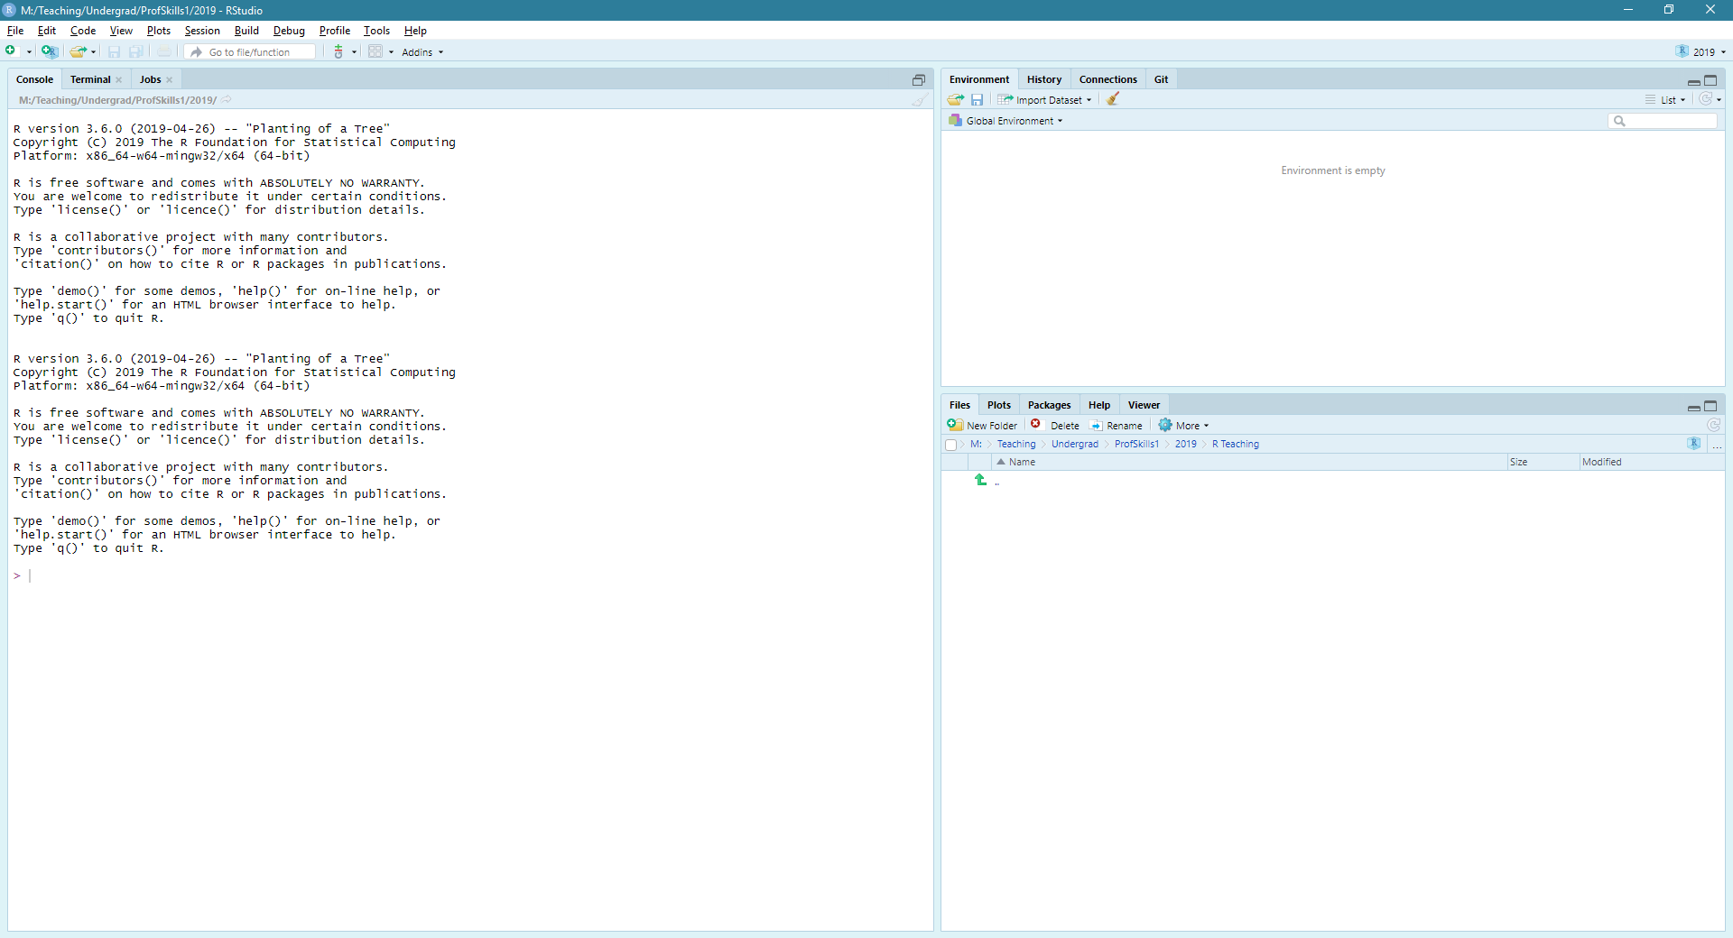
\includegraphics[width=24.07in]{images/02_install/rstud01} 

}

\caption{R Studio Overview}\label{fig:unnamed-chunk-9}
\end{figure}

\hypertarget{click-on-file-new-file-r-script}{%
\subsubsection{Click on File \textgreater{} New File\textgreater{} R Script}\label{click-on-file-new-file-r-script}}

Now your screen should look like \textbf{Figure 1.2}. You will have four panes in your window, and each pane can be dragged around or minimised. Note - you want to create a new R Script file, \textbf{not} an R Markdown or R Notebook file. We will do that next.

\begin{figure}

{\centering 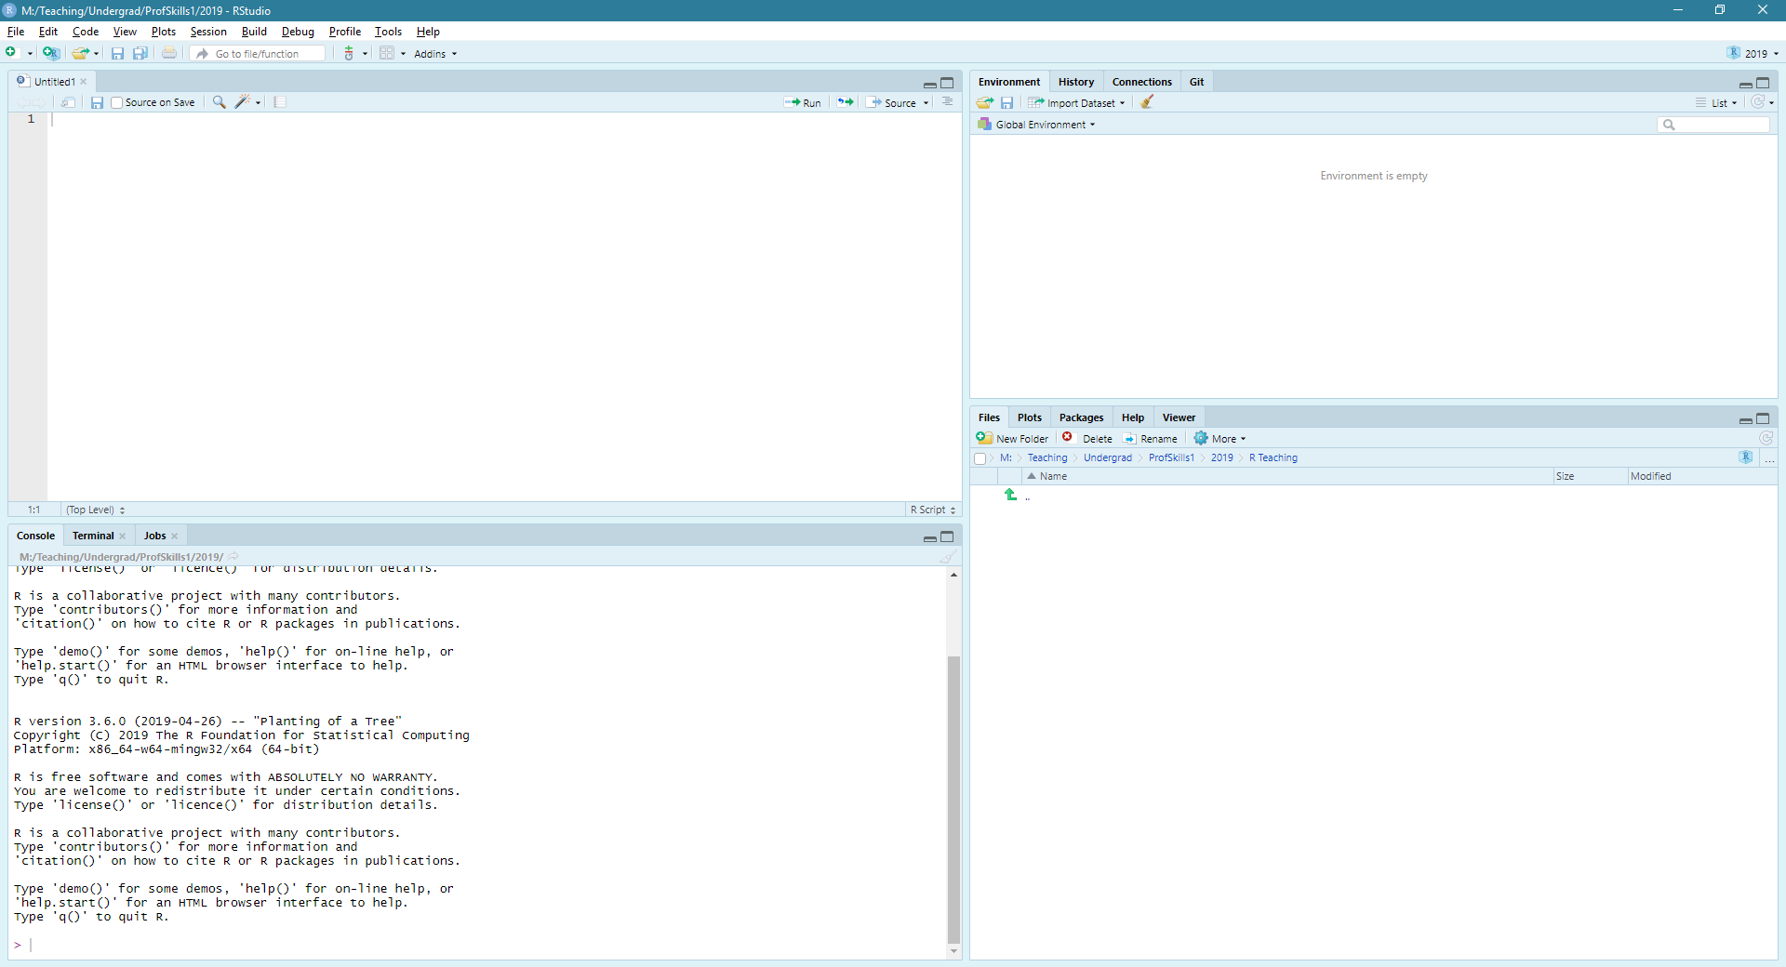
\includegraphics[width=24.81in]{images/02_install/rstud02} 

}

\caption{R Studio Overview with Script File}\label{fig:unnamed-chunk-10}
\end{figure}

\hypertarget{the-file-pane}{%
\subsubsection{The file pane}\label{the-file-pane}}

On the top left hand side of the R Studio window you can view the untitled R Script file you have just opened (\textbf{Figure 1.3}). Here you will see views of your files (mostly R Script files and R Markdown files in this book), and views of your data.

\begin{figure}

{\centering 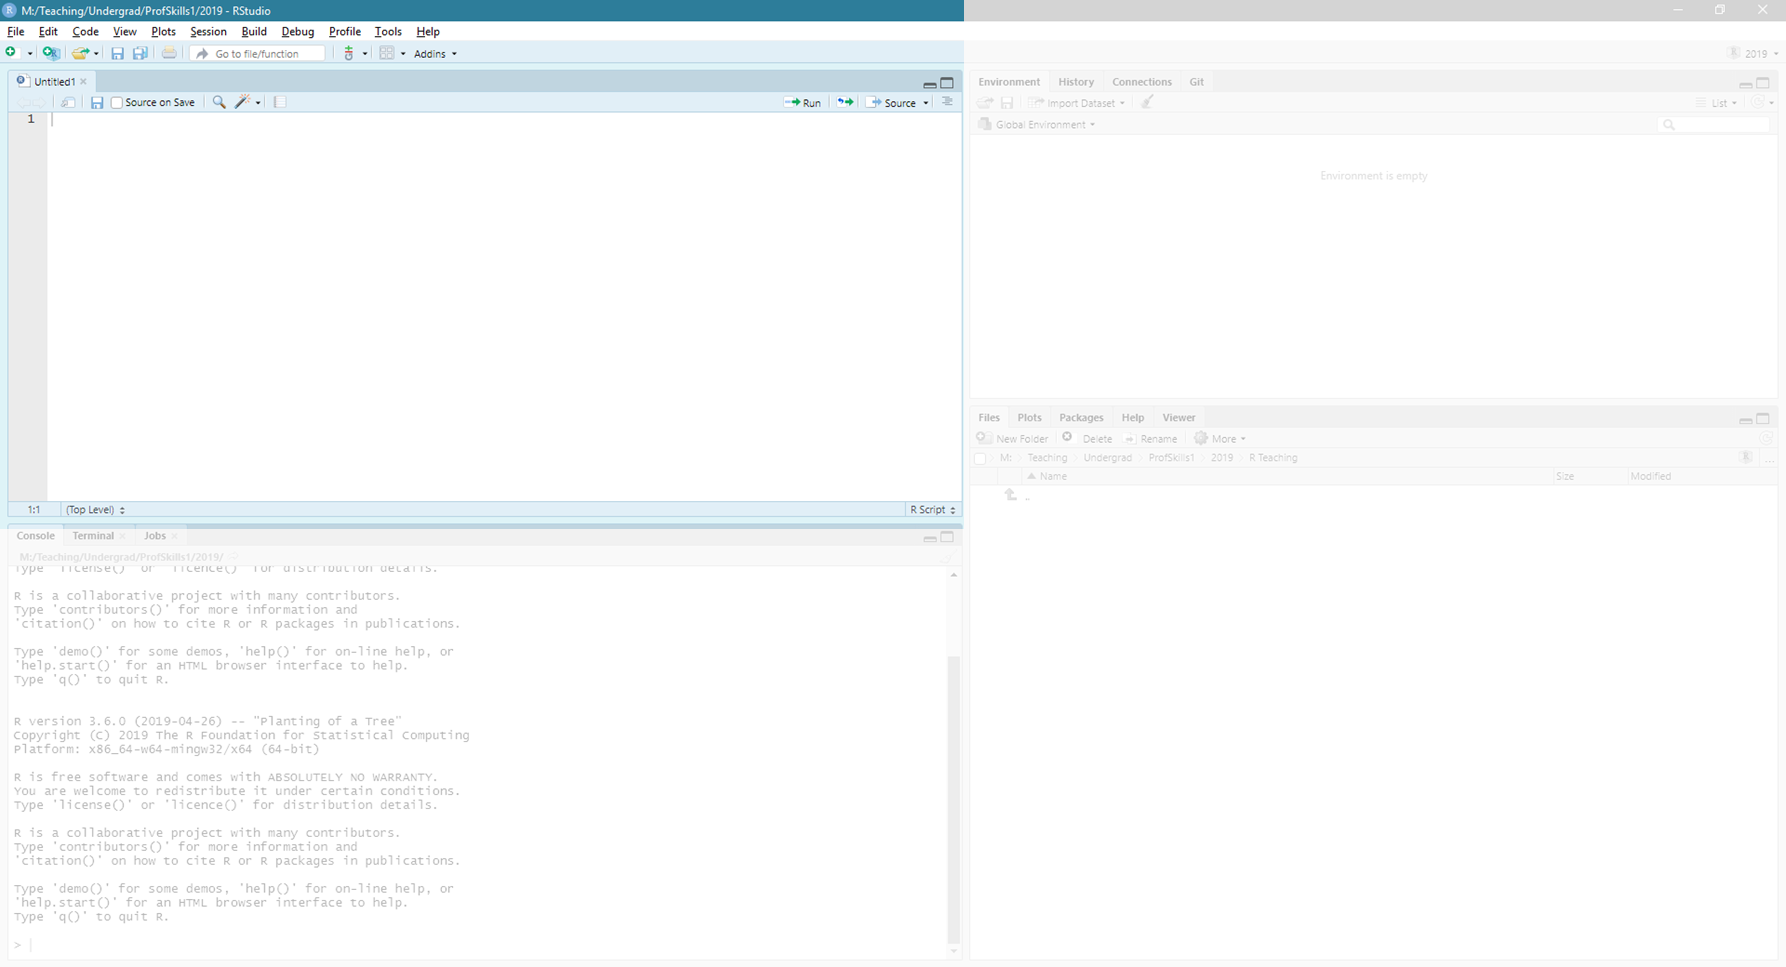
\includegraphics[width=24.81in]{images/02_install/rstud03} 

}

\caption{The active file pane}\label{fig:unnamed-chunk-11}
\end{figure}

\hypertarget{the-console}{%
\subsubsection{The console}\label{the-console}}

If you were using plain R (without R Studio) this console window is all you would see. Where you see this \textbf{\textgreater{}} symbol in the console you can type in a simple maths equation.

I recommend you type something now, perhaps \texttt{2\ +\ 2}

When you have finished typing, hit enter on your keyboard and see what the answer is.

Type \texttt{2\ +} and then hit enter. What happens? You will need to hit `escape' (`esc') on your keyboard to make the \textbf{\textgreater{}} symbol appear again.

Hitting `enter' asks R to perform the last command. Because we didn't tell R what it had to add, it kept waiting to find out what would come next.

\begin{figure}

{\centering 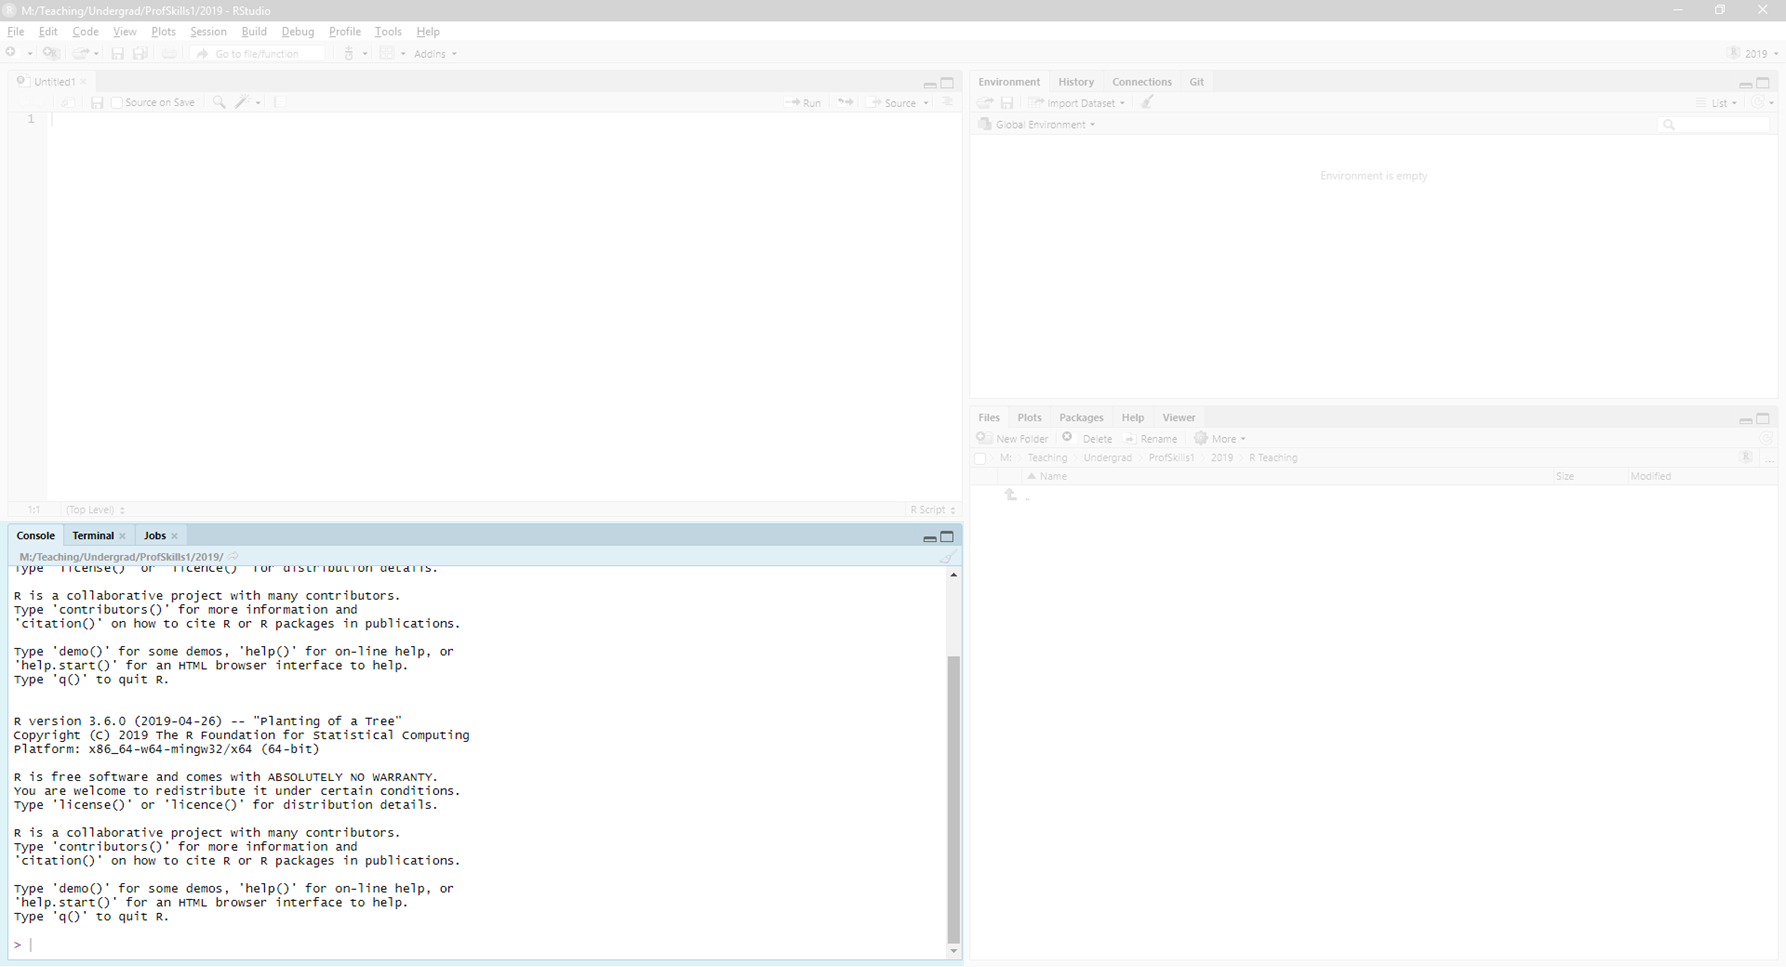
\includegraphics[width=24.81in]{images/02_install/rstud04} 

}

\caption{The console pane}\label{fig:unnamed-chunk-12}
\end{figure}

\hypertarget{the-environment-pane}{%
\subsubsection{The Environment pane}\label{the-environment-pane}}

The Environment is shown in \textbf{Figure 1.5}. At the moment, your environment will be empty. We will talk more about what goes here in \protect\hyperlink{environment}{the environment section of getting started}.

\begin{figure}

{\centering 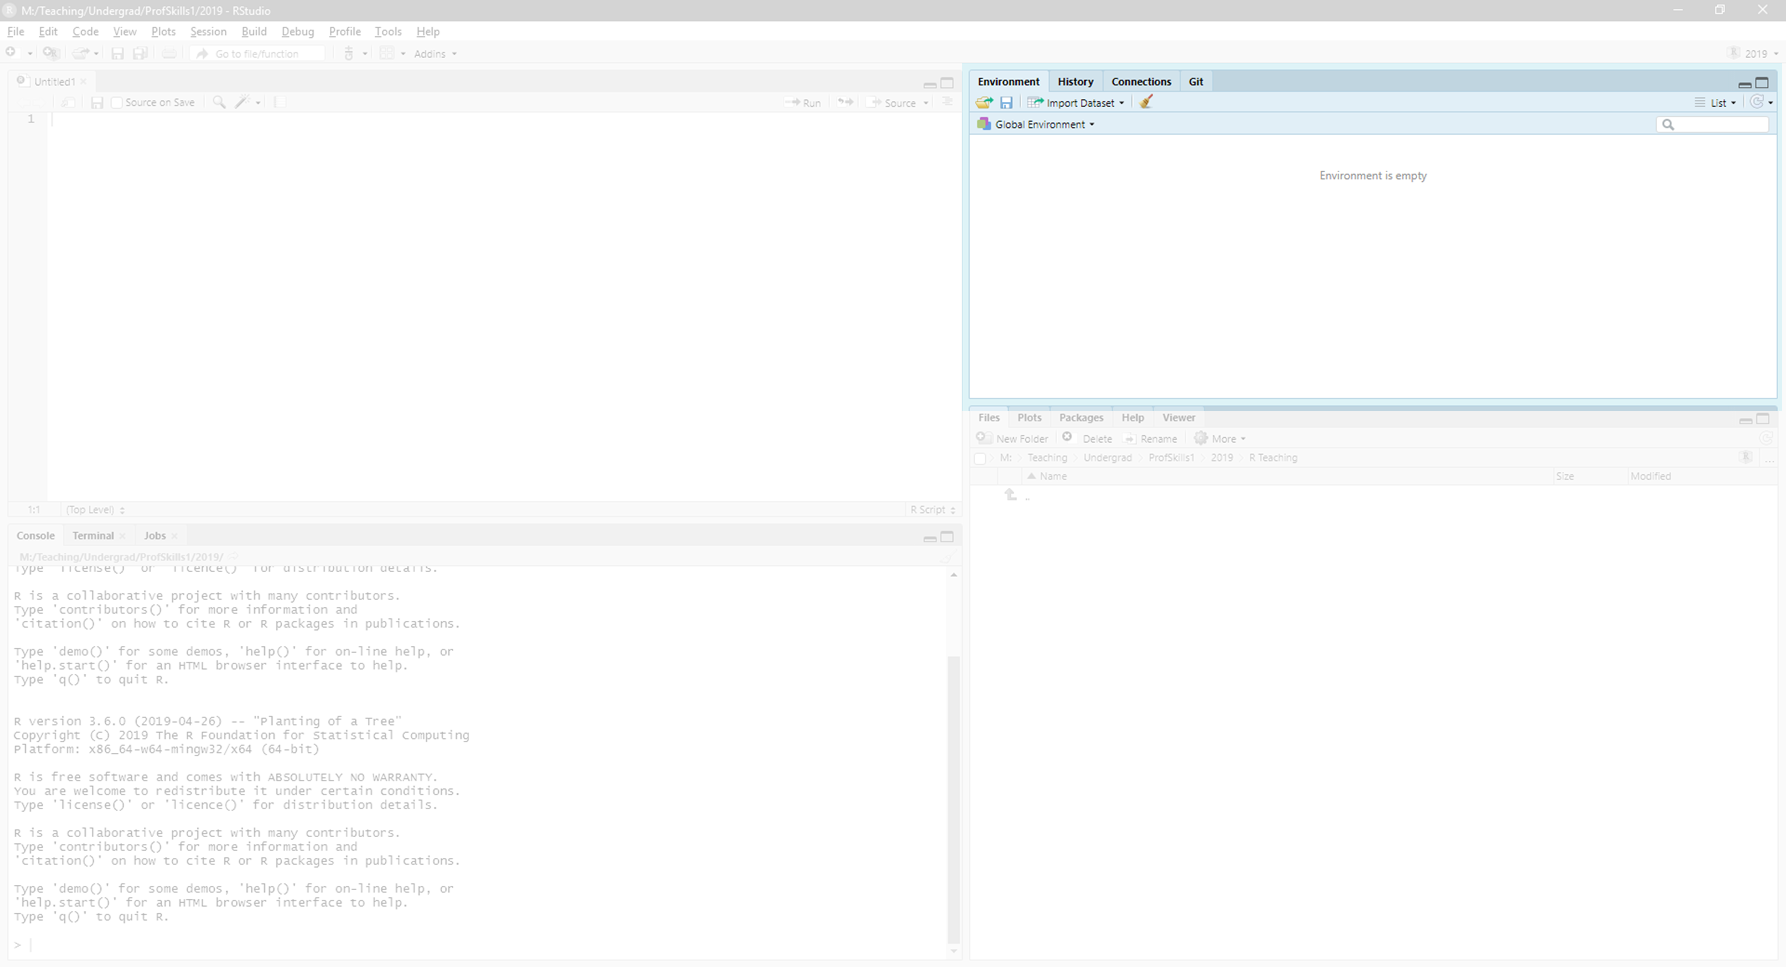
\includegraphics[width=24.81in]{images/02_install/rstud05} 

}

\caption{The environment pane}\label{fig:unnamed-chunk-13}
\end{figure}

\hypertarget{files-plots-packages-help-and-viewer}{%
\subsubsection{Files, plots, packages, help and viewer}\label{files-plots-packages-help-and-viewer}}

The final pane, shown in \textbf{Figure 1.6}, has five tabs in it by default.

These are:

\begin{itemize}
\tightlist
\item
  Files

  \begin{itemize}
  \tightlist
  \item
    Think of this like a Windows Explorer window (folder window) on your PC. It will show you all the files in your current folder and may just show your .Rproj file right now.
  \end{itemize}
\item
  Plots

  \begin{itemize}
  \tightlist
  \item
    When we start drawing charts they'll be saved here.
  \end{itemize}
\item
  Packages

  \begin{itemize}
  \tightlist
  \item
    Other wonderful people in the R Community write lots of clever code that can be `packaged' up so we can use it. Instead of writing out all the code you need to make a chart, you can use someone's package instead. We will learn more about these in \protect\hyperlink{packages}{packages}
  \end{itemize}
\item
  Help

  \begin{itemize}
  \tightlist
  \item
    If you ever get stuck with a commaned you can type \texttt{?command\_name} to view the command's documentation. Try it now by type \texttt{?summary} in the \textbf{console} window. Remember you need to press enter on your keyboard after typing the command.
  \end{itemize}
\item
  Viewer

  \begin{itemize}
  \tightlist
  \item
    This tab will show you more complicated things, like if you use R to build an html page (or a book like this one!) Ignore it for now.
  \end{itemize}
\end{itemize}

\begin{figure}

{\centering 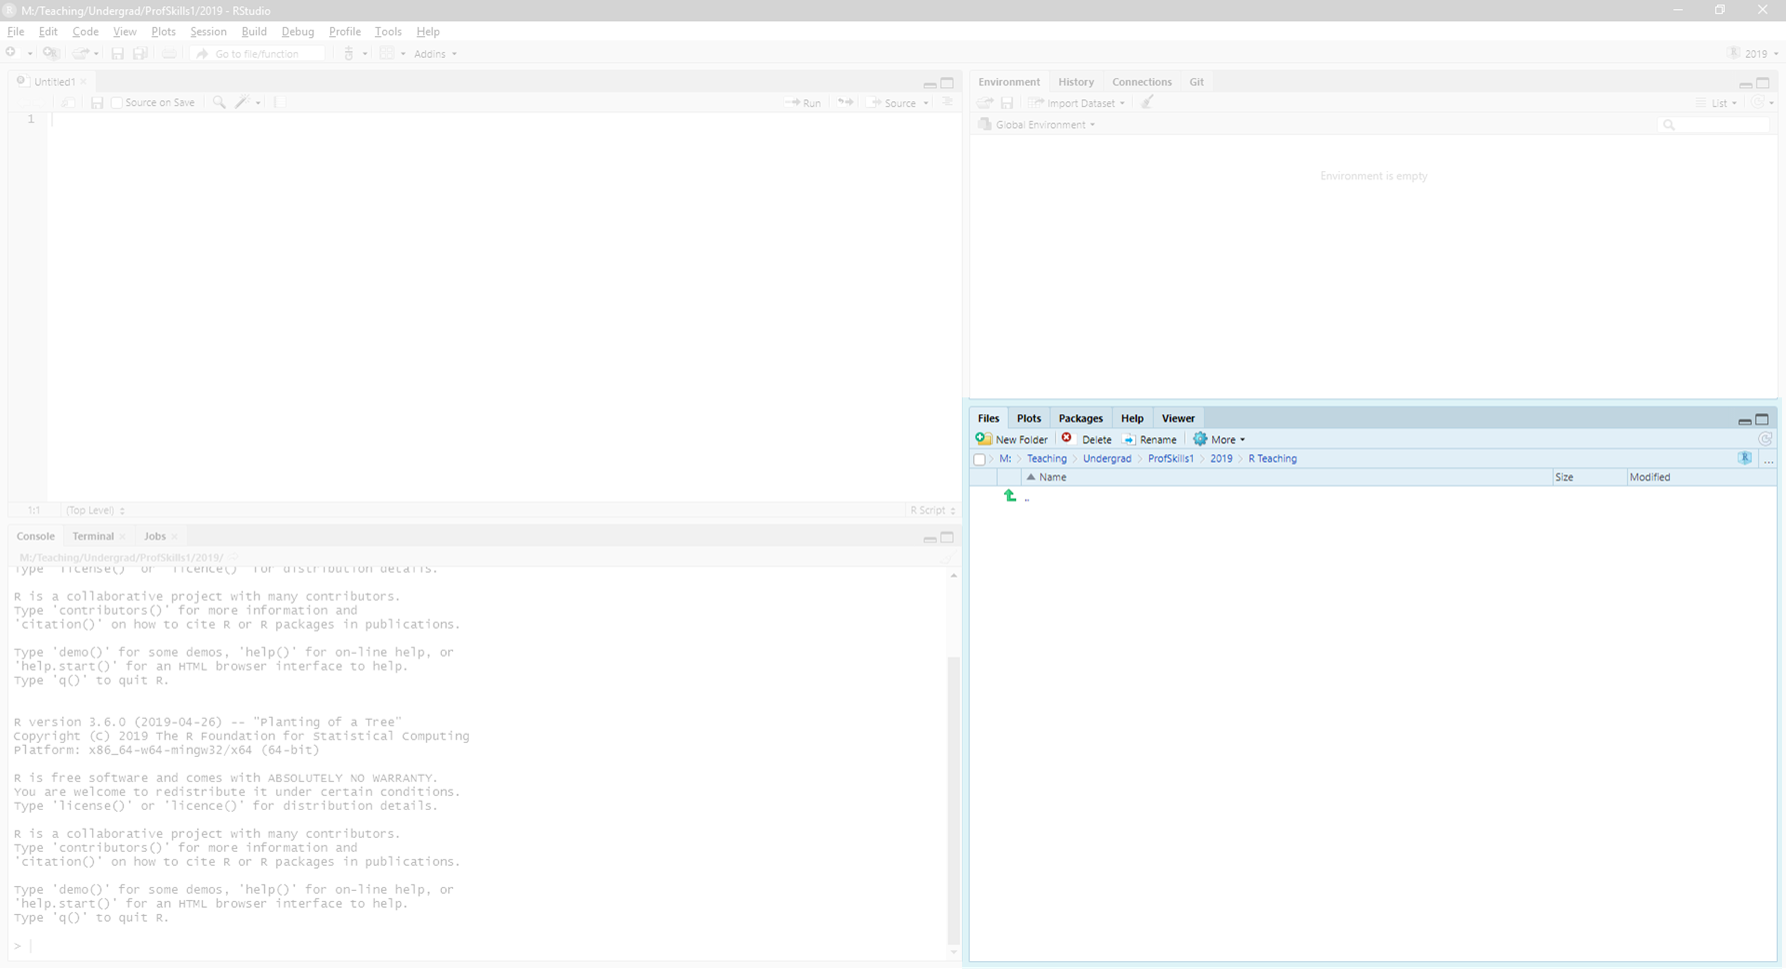
\includegraphics[width=24.81in]{images/02_install/rstud06} 

}

\caption{File, plot, package and help viewer}\label{fig:unnamed-chunk-14}
\end{figure}

\hypertarget{customisation}{%
\subsubsection{Customisation}\label{customisation}}

Data analysis is fun, and its also personal. You can customise your R Studio to look the way you want it to.

Go to \texttt{Tools\ \textgreater{}\ Global\ Options} (\textbf{Figure 1.7})

\begin{figure}

{\centering 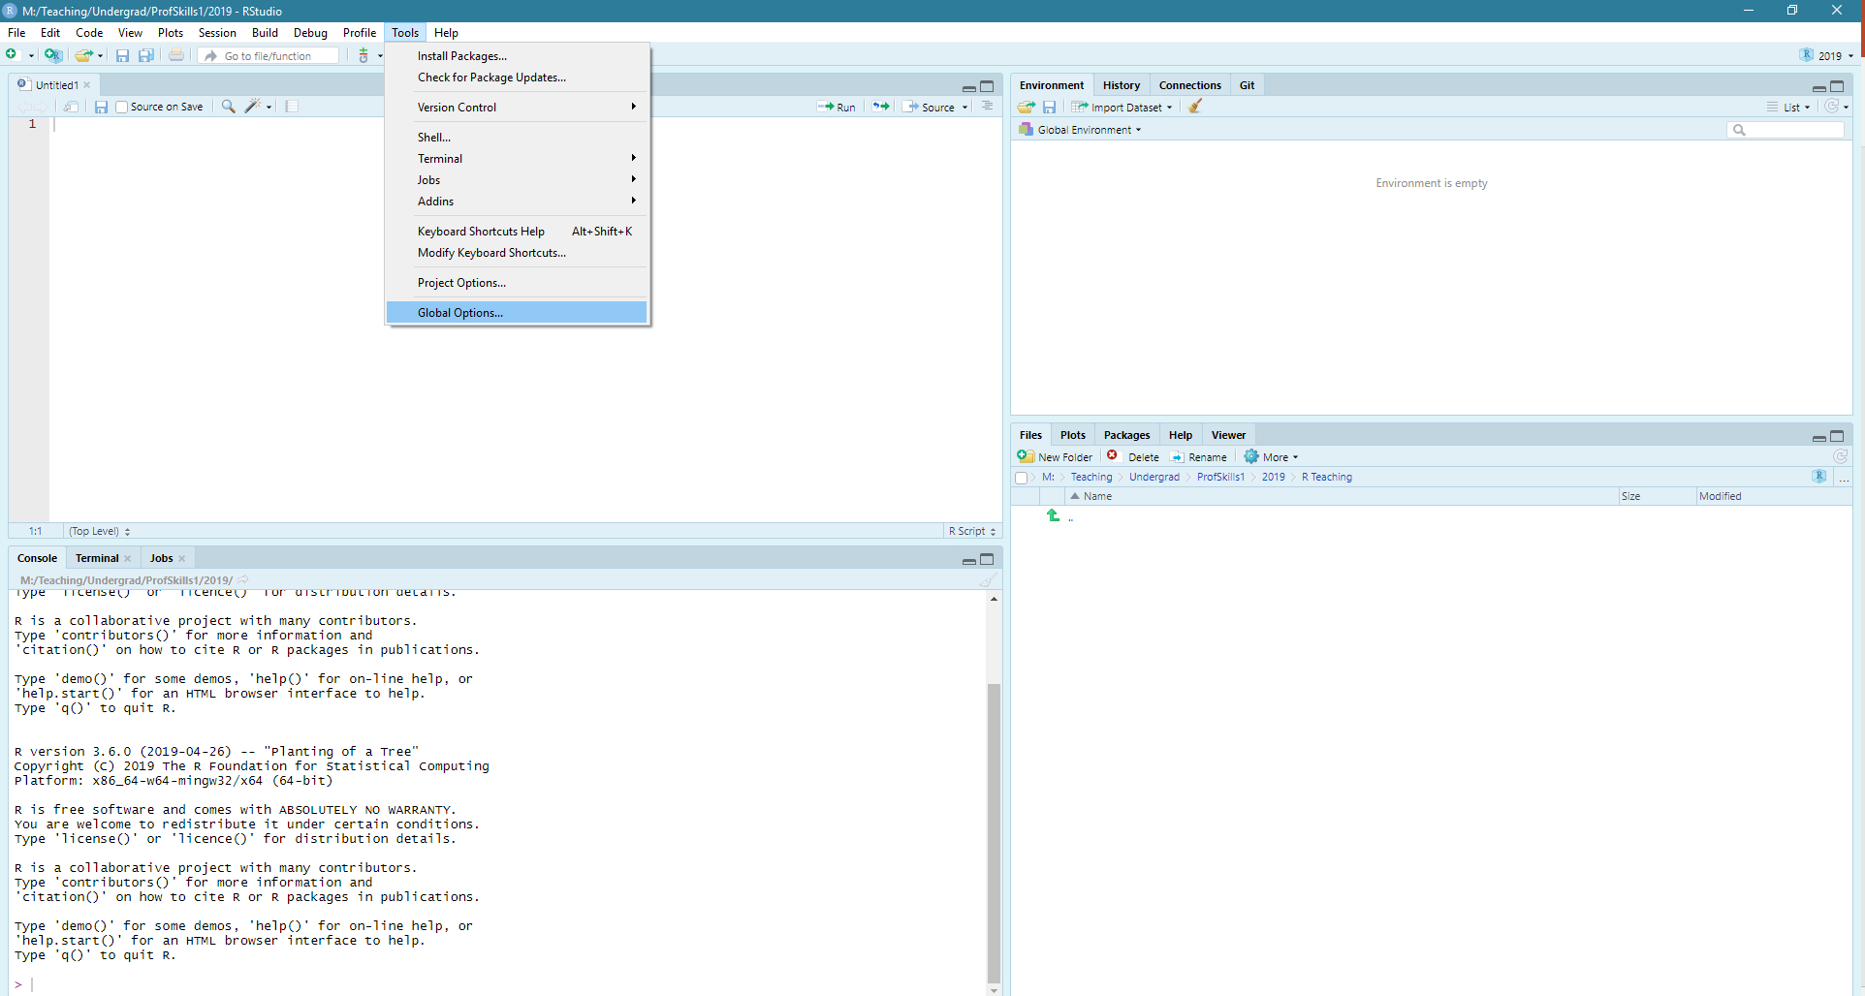
\includegraphics[width=25.9in]{images/02_install/rstud07} 

}

\caption{Global options}\label{fig:unnamed-chunk-15}
\end{figure}

And then go to \texttt{Appearance\ \textgreater{}\ Editor\ Theme} to play around and find the colour scheme, font, and R Studio Theme you like best (\textbf{Figure 1.8})

\begin{figure}

{\centering 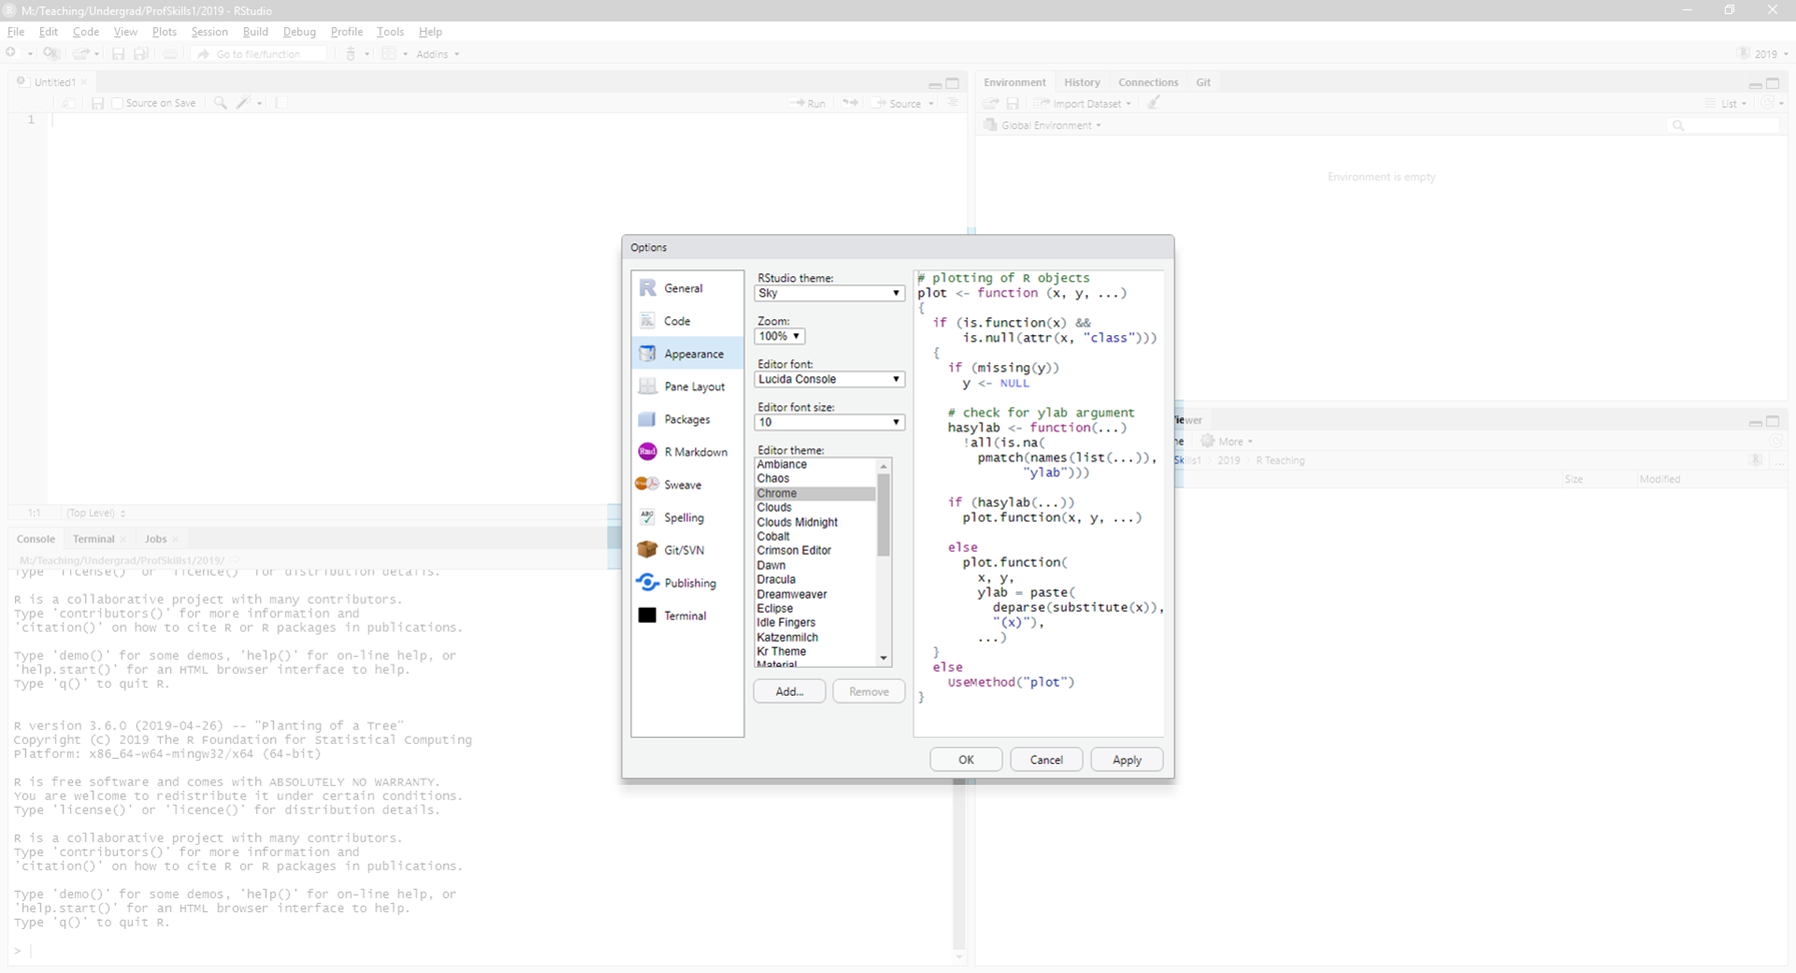
\includegraphics[width=24.94in]{images/02_install/rstud08} 

}

\caption{Global options, themes}\label{fig:unnamed-chunk-16}
\end{figure}

Personally I like the theme \texttt{XCode}, but it's your R Studio! You choose the one you like.

\hypertarget{install_rsc}{%
\section{Using the Cloud}\label{install_rsc}}

If you would like to use R Studio Cloud, you will need to create an R Studio account. This can be a whole new account, a google account, or a github account. I would recommend you get a github account (you can jump \protect\hyperlink{github}{to read why here}).

After you have logged in, you can access a workspace. A workspace is like an R Studio Project.

As of the 3rd August, 2020, R Studio Cloud is moving out of Beta and will be available to all. You should use the \textbf{Cloud Free Plan}. Again, we do not expect you to buy anything to use R or R Studio.

You will have a maximum of 15 projects you can use, and less storage space than using your own device.

\hypertarget{install_vids}{%
\section{Install R and R Studio - Video Instruction}\label{install_vids}}

If you prefer to get your resources in video format, there's an explanation of \href{https://media.ed.ac.uk/media/R+ConversationsA+Installing+R+and+R+Studio/1_q0mdj8mk/104843251}{installing R and R Studio here} and using \href{https://media.ed.ac.uk/media/R+ConversationsA+R+Studio+Online/1_ex8u0oj7/112983051}{R Studio Cloud here}.

Please note, these videos are a bit older now so you should expect to see some minor differences, e.g.~in version numbers.

\hypertarget{start}{%
\chapter{Getting Started}\label{start}}

\begin{los}
You can skip this chapter if you can:

\begin{itemize}
\item
  Use the console to input simple lines of code
\item
  Install and load a package
\item
  Recognise a function
\end{itemize}
\end{los}

To use this chapter you will need a working version of R and R Studio.

If you can open R Studio and type \texttt{2\ +\ 2} in the \textbf{console} you are good to go.

If that is confusing, you might need to jump back to \protect\hyperlink{install_rs}{installing R Studio} and the section \protect\hyperlink{navigate_rs}{navigating R Studio}.

\hypertarget{thesecret}{%
\section{The Big Secret}\label{thesecret}}

Okay. This is the Big Secret. The thing you will not believe. The most important thing you'll learn about R.

\begin{hey}
You should copy and paste other peoples' code.
\end{hey}

Yes, I'm serious. You should copy and paste and edit code you find online\footnote{If you're reading this as part of your coursework you might be panicking about plagiarism here, after all, we spend a lot of time telling you plagiarism is the worst thing you could ever do and that we'll use software to detect it. Code is a bit different. We are always trying to find the most efficient way of doing something, and so ideally you would all write code that was identical. Sadly, humans naturally differ in the way the think about problems. My job would be a lot easier if everybody thought the same. If I have set you this book as reading, I can swear to you I will never put your code through a plagiarism checker. That would be very stupid.}. In this book you should always be copying bits of code and pasting it into your console. That is why I publish the code alongside each question and demonstration.

It took me about ten years of working in R to get over my fear of copying and pasting other peoples' code. Now I even have a \href{https://github.com/jillymackay/commoncode}{repository} of all the code I use over and over so I can copy and paste my own code.

Most people will not remember code off the top of their head. This is why we use the help function (try typing \texttt{?summary} to see what it says) to look at the documentation, and resources like Stack Exchange and Google to help us (more in \protect\hyperlink{trouble}{troubleshooting}).

\hypertarget{ex_tidytuesday}{%
\subsection{Exercise}\label{ex_tidytuesday}}

You might be very skeptical here about how much I want you to be copying code. If you're not convinced, I suggest you go watch my RStats Crush the amazing \href{https://twitter.com/drob}{David Robinson} do one of his Tidy Tuesday screencasts. David Robinson has forgotten more R than I'll ever learn, and see - he still \href{https://www.youtube.com/channel/UCeiiqmVK07qhY-wvg3IZiZQ}{copies and pastes code}.

\hypertarget{projects}{%
\section{Projects}\label{projects}}

I would like to begin by creating a new project in R Studio.

\begin{itemize}
\item
  Open R Studio
\item
  Go to \texttt{File\ \textgreater{}\ New\ Project}
\item
  Set up a new project either in an existing directory (folder), or in a new one. Ignore repositories for now.
\end{itemize}

You can call this project anything you like. I recommend something short like `start'.

A R Project sits inside a folder. Everything inside that folder is part of that R Project. Let's say you have a folder called:

\texttt{mydata}

and you create an R Project called \texttt{analysis}.

The \texttt{analysis.Rproj} will live inside the \texttt{mydata} folder, and it will `see' all the data, files, and any other folders, you have in \texttt{mydata}.

Using R Studio you will get a lot better at `directory management', or knowing where you have saved things.

\hypertarget{environment}{%
\section{Environment}\label{environment}}

In your brand new project you will have a clean environment (refer back to \protect\hyperlink{navigate_rs}{Figure 2.5}). Our first exercise is going to explore what the environment really means.

\hypertarget{ex_env}{%
\subsection{Exercise - Environment}\label{ex_env}}

When we first installed R, you were typing mathematical equations into the console. Let's remind ourselves of this by running an equation now. In the console, type a long and complicated equation, then hit `enter' when you're done.

\begin{Shaded}
\begin{Highlighting}[]
\DecValTok{500} \OperatorTok{+}\StringTok{ }\DecValTok{23} \OperatorTok{/}\StringTok{ }\DecValTok{91}
\end{Highlighting}
\end{Shaded}

\begin{verbatim}
## [1] 500.2527
\end{verbatim}

If this was a calculation we often ran, we might want to save the answer. We can do this by using the \textbf{assign} symbol \textbf{\textless{}-}.

For example, if we type this:

\begin{Shaded}
\begin{Highlighting}[]
\NormalTok{x <-}\StringTok{ }\DecValTok{500} \OperatorTok{+}\StringTok{ }\DecValTok{23} \OperatorTok{/}\StringTok{ }\DecValTok{91}
\end{Highlighting}
\end{Shaded}

\ldots{} you will see that we simply get a new line returned. We don't get the answer. However, in your environment you will see under the heading `Values', a new thing called \texttt{x}.

Enter the following code:

\begin{Shaded}
\begin{Highlighting}[]
\NormalTok{x}
\end{Highlighting}
\end{Shaded}

\begin{verbatim}
## [1] 500.2527
\end{verbatim}

R remembers what x is and recalled it. This is useful if we want to do more with \texttt{x} after we've calculated it.

\begin{Shaded}
\begin{Highlighting}[]
\NormalTok{x }\OperatorTok{/}\DecValTok{100}
\end{Highlighting}
\end{Shaded}

\begin{verbatim}
## [1] 5.002527
\end{verbatim}

As well as values, we can ask R to remember a string of text as well. Try this:

\begin{Shaded}
\begin{Highlighting}[]
\NormalTok{hello <-}\StringTok{ "Computers always print 'Hello World!' but we never say hello back"}


\KeywordTok{print}\NormalTok{(hello)}
\end{Highlighting}
\end{Shaded}

\begin{verbatim}
## [1] "Computers always print 'Hello World!' but we never say hello back"
\end{verbatim}

But R is very fussy. What happens if you run this code:

\begin{Shaded}
\begin{Highlighting}[]
\KeywordTok{print}\NormalTok{(HELLO)}
\end{Highlighting}
\end{Shaded}

You see, R is \textbf{case sensitive}, meaning we have to be careful to always type things the same. This is one of the reasons why R Studio is really handy, because you can see what you've saved in your environment.

Now type this:

\begin{Shaded}
\begin{Highlighting}[]
\NormalTok{hello <-}\StringTok{ "Hello, R!"}
\end{Highlighting}
\end{Shaded}

Take a guess what is going to happen before you type the next line. Were you right?

\begin{Shaded}
\begin{Highlighting}[]
\KeywordTok{print}\NormalTok{(hello)}
\end{Highlighting}
\end{Shaded}

\begin{verbatim}
## [1] "Hello, R!"
\end{verbatim}

\hypertarget{ex_func}{%
\subsection{Exercise - Functions}\label{ex_func}}

\hypertarget{the-basic-function}{%
\subsubsection{The Basic Function}\label{the-basic-function}}

A function is a handy way to bundle together some lines of code. David Robinson \href{https://twitter.com/drob/status/928447584712253440?s=20}{says that} if you run a few lines more than twice you should write a function to do it instead.

I'm going to contradict myself now. Functions are really important in R, but I'm not going to ask you to write one anywhere else but in this exercise. Most things in this book I expect you to practice over and over, but functions are useful to understand \protect\hyperlink{packages}{packages}, and that's why we're going to talk about them now.

Let's create a function to make R welcome us. Copy and paste this code into a new script file (you may want to save it as your functions example), and then run it.

\begin{Shaded}
\begin{Highlighting}[]
\NormalTok{mynameis <-}\StringTok{ }\ControlFlowTok{function}\NormalTok{ (name) \{}
  \KeywordTok{print}\NormalTok{ (}\KeywordTok{paste0}\NormalTok{(}\StringTok{"Hello, "}\NormalTok{, name, }\StringTok{", how are you today?"}\NormalTok{))}
\NormalTok{\}}
\KeywordTok{mynameis}\NormalTok{ (}\StringTok{"Jill"}\NormalTok{)}
\end{Highlighting}
\end{Shaded}

\begin{verbatim}
## [1] "Hello, Jill, how are you today?"
\end{verbatim}

\textbf{What is this code saying?}

\begin{translate}
Create a new thing called \texttt{mynameis}

Give (\texttt{\textless{}-}) \texttt{mynameis} the \texttt{function}
purpose. Everything inside the curly brackets \texttt{\{\}} is the
function.

The \texttt{function} should make a new thing called \texttt{name}.

The \texttt{function} should \texttt{print} the result of pasting a
string (\texttt{paste0}) of things, the words \texttt{Hello,}, whatever
you said \texttt{name} should be, and \texttt{,\ how\ are\ you\ today?}.
\end{translate}

You may have noticed that, just like when we were assigning \texttt{x} a value, we now have something in our environment called \texttt{mynameis}.

Whenever we type \texttt{mynameis("Jill")} into the console, or execute that line in a script file, R knows it should look to the environment and run the code that's been bundled up into that package.

For example, we could make R welcome us in exactly the same way by typing:

\begin{Shaded}
\begin{Highlighting}[]
\KeywordTok{print}\NormalTok{ (}\KeywordTok{paste0}\NormalTok{(}\StringTok{"Hello, "}\NormalTok{, }\StringTok{"Jill"}\NormalTok{, }\StringTok{", how are you today?"}\NormalTok{))}
\end{Highlighting}
\end{Shaded}

\begin{verbatim}
## [1] "Hello, Jill, how are you today?"
\end{verbatim}

But we would need to change the name every time we wanted welcome a new user. \textbf{We are lazy, so we use the function to reduce the amount of things we need to change to get a different outcome.}

Functions make our code more standardised. If we all define the \texttt{mynameis} function at the start of our documentation, we don't need to worry about accidentally deleting an important character in the code. This is especially important as we like to copy-paste code when we need to.

Most scientists will probably not write their own functions, but you should know how they work.

\hypertarget{packages}{%
\section{Packages}\label{packages}}

If people write very good and useful functions, they usually want to share them. They can do this with packages.

There are packages for everything, packages for drawing maps, packages for analysing data, packages for suggesting how to analyse your data, packages to give you more data, packages for tidying your data . . . this is one of the reasons we might all have different bits of code. There can be lots of ways to do something.

\hypertarget{ex_packages}{%
\subsection{Exercise - Install and Load a Package}\label{ex_packages}}

Packages work in two stages. The very first time you need a package you need to install it. Then, every time you start R you need to load the package into your livrary.

To install a package you need to type \texttt{install.package("package\_name")}.

To load it into your library you need to type \texttt{library(package\_name)}.

When you load a package from your library it goes into a special hidden environment where you can access all the functions that the package has written for you.

For example, we will make great use of the \texttt{tidyverse} package in this book. You need to start by installing it with:

\begin{Shaded}
\begin{Highlighting}[]
\KeywordTok{install.packages}\NormalTok{(}\StringTok{"tidyverse"}\NormalTok{)}
\end{Highlighting}
\end{Shaded}

And when it has finished downloading, you need to type:

\begin{Shaded}
\begin{Highlighting}[]
\KeywordTok{library}\NormalTok{(tidyverse)}
\end{Highlighting}
\end{Shaded}

to load it. You'll see that nothing has appeared in your Environment, but actually you have a whole host of new functions \& data you can play with. For example:

\begin{Shaded}
\begin{Highlighting}[]
\KeywordTok{slice}\NormalTok{(starwars)}
\end{Highlighting}
\end{Shaded}

Which should give you this:

\begin{verbatim}
## # A tibble: 87 x 14
##    name     height  mass hair_color  skin_color  eye_color birth_year sex   gender homeworld species films vehicles starships
##    <chr>     <int> <dbl> <chr>       <chr>       <chr>          <dbl> <chr> <chr>  <chr>     <chr>   <lis> <list>   <list>   
##  1 Luke Sk~    172    77 blond       fair        blue            19   male  mascu~ Tatooine  Human   <chr~ <chr [2~ <chr [2]>
##  2 C-3PO       167    75 <NA>        gold        yellow         112   none  mascu~ Tatooine  Droid   <chr~ <chr [0~ <chr [0]>
##  3 R2-D2        96    32 <NA>        white, blue red             33   none  mascu~ Naboo     Droid   <chr~ <chr [0~ <chr [0]>
##  4 Darth V~    202   136 none        white       yellow          41.9 male  mascu~ Tatooine  Human   <chr~ <chr [0~ <chr [1]>
##  5 Leia Or~    150    49 brown       light       brown           19   fema~ femin~ Alderaan  Human   <chr~ <chr [1~ <chr [0]>
##  6 Owen La~    178   120 brown, grey light       blue            52   male  mascu~ Tatooine  Human   <chr~ <chr [0~ <chr [0]>
##  7 Beru Wh~    165    75 brown       light       blue            47   fema~ femin~ Tatooine  Human   <chr~ <chr [0~ <chr [0]>
##  8 R5-D4        97    32 <NA>        white, red  red             NA   none  mascu~ Tatooine  Droid   <chr~ <chr [0~ <chr [0]>
##  9 Biggs D~    183    84 black       light       brown           24   male  mascu~ Tatooine  Human   <chr~ <chr [0~ <chr [1]>
## 10 Obi-Wan~    182    77 auburn, wh~ fair        blue-gray       57   male  mascu~ Stewjon   Human   <chr~ <chr [1~ <chr [5]>
## # ... with 77 more rows
\end{verbatim}

Now we have a new dataset (\texttt{starwars}) and a new thing we can do (\texttt{slice} the top of the data). We will talk much more about \texttt{tidyverse} in the \protect\hyperlink{data}{data chapter}.

\begin{hey}
You will often get warnings in R when you type these code blocks. To
keep the book tidy, I have suppressed (hidden) the warnings in this
book. Don't worry about them - they're usually just trying to keep
packages compatibile with older versions of R
\end{hey}

\hypertarget{scripts_rmd}{%
\section{R Markdown vs R Scripts}\label{scripts_rmd}}

In R Studio you can use R Script files and R Markdown files to save your work. Both of these files can be created, edited, saved, and opened in your R Project file. You can send R Script and R Markdown files to other people, so they can edit and share your code too.

If you are reading this book as part of coursework I've set you, you will likely have an assignment where you neeed to download and edit an R Markdown file, then send it back to me.

\hypertarget{r-scripts}{%
\subsection{R Scripts}\label{r-scripts}}

R script files are great for testing out small chunks of code on their own.

Go to \texttt{File\ \textgreater{}\ New\ File\ \textgreater{}\ R\ Script} or press \texttt{Ctrl\ +\ Shift\ +\ N} to open one.

Everything you type in an R script file is executable code.

Unlike working in the \textbf{console}, you can type multiple lines of code in an R script, and run each one by hitting \texttt{ctrl\ +\ enter}.

You \textbf{can't type} plain text in an R Script file. Text has to be annotated by the comment symbol (\texttt{\#})

\begin{Shaded}
\begin{Highlighting}[]
\CommentTok{# In an R script file - you can write comments}
\CommentTok{# Which always begin with a hashtag}

\CommentTok{# Comments can be useful to say things like what date you wrote the script on,}
\CommentTok{# or what you were trying to do. }

\KeywordTok{print}\NormalTok{(}\StringTok{"You can also use script files to write multiple lines of code"}\NormalTok{)}

\KeywordTok{print}\NormalTok{(}\StringTok{"and edit those lines of code"}\NormalTok{)}


\CommentTok{# before you run them by pressing ctrl + enter at the same time  when your cursor is on that line. }
\end{Highlighting}
\end{Shaded}

\hypertarget{r-markdown}{%
\subsection{R Markdown}\label{r-markdown}}

R Markdown allows you to combine code with actual text. This book was written in R Markdown

In R Markdown you can have a text chunk like this one.

And follow that with code, bracketed with three ticks like this:
```\{r\}

print(``followed by code like this'')

```

\begin{verbatim}
## [1] "followed by code like this"
\end{verbatim}

\href{https://rstudio.com/wp-content/uploads/2015/02/rmarkdown-cheatsheet.pdf}{There is a great R Markdown cheatsheet from R Studio here}. I had this printed out and hung above my desk for years.

\hypertarget{video_rmd}{%
\subsection{A video on R Markdown}\label{video_rmd}}

If you would like to watch me using R Markdown, you're in luck! Theres \href{https://media.ed.ac.uk/media/R+ConversationsA+Intro+to+R+Markdown/1_td0q33v8/112983051}{a video here}.

\hypertarget{video_env}{%
\section{Video Introductions}\label{video_env}}

There is a short introduction to R and R Studio in Video format here:

\begin{itemize}
\item
  \href{https://media.ed.ac.uk/media/R+ConversationsA+Intro+to+R+Studio+1/1_aox3in51/112983051}{Video 1}
\item
  \href{https://media.ed.ac.uk/media/R+ConversationsA+Intro+to+R+Studio+2/1_vm1bylon}{Video 2}
\end{itemize}

\hypertarget{data}{%
\chapter{Data}\label{data}}

\begin{los}
You can skip this chapter if you:

\begin{itemize}
\item
  Are comfortable working with dataframes and tibbles
\item
  Know about and are comfortable using some of R's inbuilt data packages
\item
  Are comfortable loading .csv and .xlsx files into R
\end{itemize}
\end{los}

\hypertarget{packages-for-this-chapter}{%
\section{Packages for this chapter}\label{packages-for-this-chapter}}

In this chapter you'll want the following packages loaded in your R session. At the start, you will need to run the following code. Remember if you don't have a package you can install it with the \texttt{install.package("package\_name")} command.

\begin{Shaded}
\begin{Highlighting}[]
\KeywordTok{library}\NormalTok{(tidyverse)}
\KeywordTok{library}\NormalTok{(readxl)}
\end{Highlighting}
\end{Shaded}

\hypertarget{data_builtin}{%
\section{Built In Data}\label{data_builtin}}

Many packages, such as the \texttt{tidyverse} package, and the default\footnote{`Default' here means one you won't need to install or load into the library} \texttt{datasets} package come with data in them. These datasets can be really useful for testing code that you're unfamiliar with, because you know what the data should look like, and how it should perform.

Some common datasets are:

\begin{itemize}
\item
  \texttt{mpg}

  \begin{itemize}
  \tightlist
  \item
    Fuel economy data from 1999 to 2008 for 38 popular models of cars
  \end{itemize}
\item
  \texttt{ChickWeight}
\item
  Weight versus age of chicks on different diets
\item
  \texttt{starwars}

  \begin{itemize}
  \tightlist
  \item
    Name, height, weight, age, and other characteristics of Star Wars characters
  \end{itemize}
\item
  \texttt{iris}

  \begin{itemize}
  \tightlist
  \item
    The measurements (in cm) of the sepal length and width and petal length and width of 50 flowers in 3 species of iris
  \end{itemize}
\end{itemize}

There are many, many more. You can explore some of them by typing \texttt{datasets::} into the console and instead of pressing `enter', scroll the menu that pops up to help you autocomplete your command.

\begin{hey}
You might wonder, what's the \texttt{::} in the \texttt{datasets::}
command. The \texttt{::} is very useful and tells R to look inside the
\texttt{datasets} package without having to actually load it into your
library which can be very quick and easy
\end{hey}

\hypertarget{ex_inbuiltdata}{%
\section{Exercise}\label{ex_inbuiltdata}}

For our first exercise we are going to look at some of the inbuilt datasets.

What happens when you enter the following code\footnote{If its not working - are you sure you have spelled it with a capital \texttt{View}?} into the console?

\begin{Shaded}
\begin{Highlighting}[]
\KeywordTok{View}\NormalTok{(mpg)}
\end{Highlighting}
\end{Shaded}

You should see something like \textbf{Figure 3.1}

\begin{figure}

{\centering 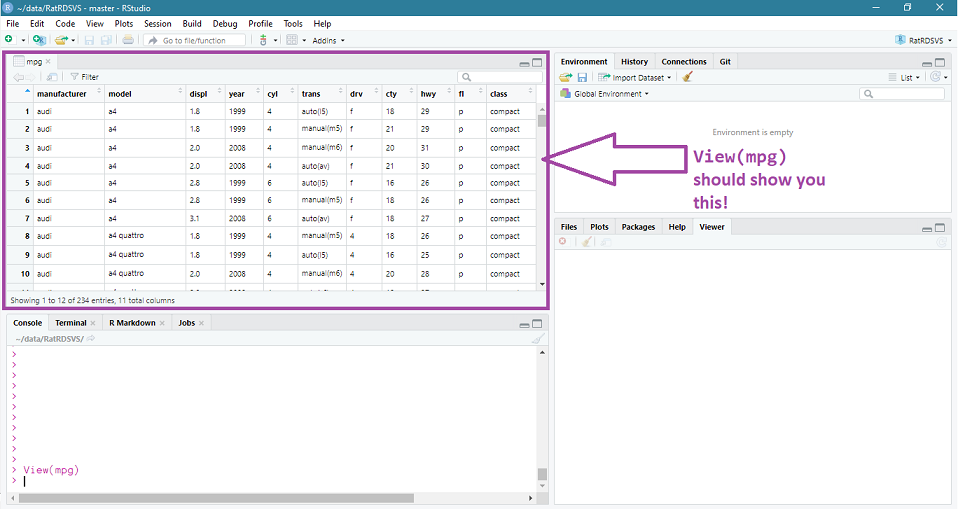
\includegraphics[width=13.31in]{images/03_data/rstud01} 

}

\caption{The result of the 'View(mpg)' command}\label{fig:unnamed-chunk-42}
\end{figure}

The \texttt{View()} command is very handy for getting a quick window onto what data looks like. Unfortunately, the \texttt{View()} command only really works for \textbf{you} getting a look at your data. If you wanted to share your code, you would be better using a command which prints some of the data into the console.

So - what functions will tell R to print data into the console?

You can view the top of a dataset with \texttt{head()}

\begin{Shaded}
\begin{Highlighting}[]
 \KeywordTok{head}\NormalTok{(mpg)}
\end{Highlighting}
\end{Shaded}

\begin{verbatim}
## # A tibble: 6 x 11
##   manufacturer model displ  year   cyl trans      drv     cty   hwy fl    class  
##   <chr>        <chr> <dbl> <int> <int> <chr>      <chr> <int> <int> <chr> <chr>  
## 1 audi         a4      1.8  1999     4 auto(l5)   f        18    29 p     compact
## 2 audi         a4      1.8  1999     4 manual(m5) f        21    29 p     compact
## 3 audi         a4      2    2008     4 manual(m6) f        20    31 p     compact
## 4 audi         a4      2    2008     4 auto(av)   f        21    30 p     compact
## 5 audi         a4      2.8  1999     6 auto(l5)   f        16    26 p     compact
## 6 audi         a4      2.8  1999     6 manual(m5) f        18    26 p     compact
\end{verbatim}

Note that this code has produced an output block. Unlike \texttt{View()} where I had to share a screengrab to show you what the output of the code was. This is why \texttt{head()} is a lot more reproducible than \texttt{View()} and should be your default for code sharing. See more about this in \protect\hyperlink{workflows}{workflows}.

Unsurprisingly we can also view the bottom of a dataset with \ldots{}

\begin{Shaded}
\begin{Highlighting}[]
\KeywordTok{tail}\NormalTok{(mpg)}
\end{Highlighting}
\end{Shaded}

\begin{verbatim}
## # A tibble: 6 x 11
##   manufacturer model  displ  year   cyl trans      drv     cty   hwy fl    class  
##   <chr>        <chr>  <dbl> <int> <int> <chr>      <chr> <int> <int> <chr> <chr>  
## 1 volkswagen   passat   1.8  1999     4 auto(l5)   f        18    29 p     midsize
## 2 volkswagen   passat   2    2008     4 auto(s6)   f        19    28 p     midsize
## 3 volkswagen   passat   2    2008     4 manual(m6) f        21    29 p     midsize
## 4 volkswagen   passat   2.8  1999     6 auto(l5)   f        16    26 p     midsize
## 5 volkswagen   passat   2.8  1999     6 manual(m5) f        18    26 p     midsize
## 6 volkswagen   passat   3.6  2008     6 auto(s6)   f        17    26 p     midsize
\end{verbatim}

Another very useful way to look at a dataset is with the \texttt{summary()} function, which takes its best guess at how to summarise each variable in the dataset.

\begin{Shaded}
\begin{Highlighting}[]
\KeywordTok{summary}\NormalTok{(mpg)}
\end{Highlighting}
\end{Shaded}

\begin{verbatim}
##  manufacturer          model               displ            year           cyl           trans               drv           
##  Length:234         Length:234         Min.   :1.600   Min.   :1999   Min.   :4.000   Length:234         Length:234        
##  Class :character   Class :character   1st Qu.:2.400   1st Qu.:1999   1st Qu.:4.000   Class :character   Class :character  
##  Mode  :character   Mode  :character   Median :3.300   Median :2004   Median :6.000   Mode  :character   Mode  :character  
##                                        Mean   :3.472   Mean   :2004   Mean   :5.889                                        
##                                        3rd Qu.:4.600   3rd Qu.:2008   3rd Qu.:8.000                                        
##                                        Max.   :7.000   Max.   :2008   Max.   :8.000                                        
##       cty             hwy             fl               class          
##  Min.   : 9.00   Min.   :12.00   Length:234         Length:234        
##  1st Qu.:14.00   1st Qu.:18.00   Class :character   Class :character  
##  Median :17.00   Median :24.00   Mode  :character   Mode  :character  
##  Mean   :16.86   Mean   :23.44                                        
##  3rd Qu.:19.00   3rd Qu.:27.00                                        
##  Max.   :35.00   Max.   :44.00
\end{verbatim}

The \texttt{summary()} function highlights an important aspect of R - it knows the difference between numbers and characters. In the output block we can see that \texttt{manufacturer} is given the \texttt{Class} \texttt{character}. R knows it can't create a mean and a median from this data, so it simply tells you the \texttt{Length} of that data instead. What do you think the 234 refers to here? Answer in the footnote\footnote{The Length of these variables is the number of rows in each one, which for this case is the same because this is a nice, tidy dataset}.

\hypertarget{created_data}{%
\section{Data you create}\label{created_data}}

Sometimes you will want to test something on pretend data, or run something on a very small dataset. In these cases, we can create a dataset in our environment. This can be really useful for \protect\hyperlink{trouble}{troubleshooting} because you can create data that shows your problem, and this is easier to share with others.

For example, lets say we we were interested in this idea that R only sees \texttt{manufacturer} in \texttt{mpg} as a string of letters. How can we tell R that \texttt{manufacturer} is in fact a category? We can test on a smaller, simpler dataset.

\hypertarget{ex_createdata}{%
\section{Exercise - Creating data}\label{ex_createdata}}

We are going to use a new function here called \texttt{tibble} which will make a dataframe quickly and easily. Before when we were typing things like \texttt{x\ \textless{}-\ 1}, we created a single thing in the environment. Now we want to create multiple thing (rows and columns) and that's what the \texttt{tibble} function will do.

Try the following and watch what happens in your environment (you'll need the \texttt{tidyverse} loaded - see \protect\hyperlink{data}{above})

\begin{Shaded}
\begin{Highlighting}[]
\NormalTok{dat <-}\StringTok{ }\KeywordTok{tibble}\NormalTok{(}\DataTypeTok{x =} \KeywordTok{c}\NormalTok{(}\DecValTok{1}\NormalTok{, }\DecValTok{2}\NormalTok{, }\DecValTok{3}\NormalTok{, }\DecValTok{4}\NormalTok{, }\DecValTok{5}\NormalTok{, }\DecValTok{6}\NormalTok{),}
              \DataTypeTok{y =} \KeywordTok{c}\NormalTok{(}\StringTok{"A"}\NormalTok{, }\StringTok{"B"}\NormalTok{, }\StringTok{"A"}\NormalTok{, }\StringTok{"B"}\NormalTok{, }\StringTok{"A"}\NormalTok{, }\StringTok{"B"}\NormalTok{))}
\end{Highlighting}
\end{Shaded}

You can \texttt{View(dat)} to look at this (or use \texttt{head(dat)}). Let's try and replicate our weird \texttt{summary(mpg)} character issue.

\begin{Shaded}
\begin{Highlighting}[]
\KeywordTok{summary}\NormalTok{(dat)}
\end{Highlighting}
\end{Shaded}

\begin{verbatim}
##        x             y            
##  Min.   :1.00   Length:6          
##  1st Qu.:2.25   Class :character  
##  Median :3.50   Mode  :character  
##  Mean   :3.50                     
##  3rd Qu.:4.75                     
##  Max.   :6.00
\end{verbatim}

We \textbf{can} replicate the issue. You can see that the \texttt{y} variable has the \texttt{class:\ Character}. What can we do about it?

We essentially want to tell R that \texttt{y} is not a character, but a factor\footnote{A factor is also called a categorical variable, or a grouping variable. If you're not sure you know what a factor is, \href{https://en.wikipedia.org/wiki/Categorical_variable}{wiki} is a good place to review}.

We can ask R more directly what \texttt{y} is by telling it exactly where to look.

\begin{Shaded}
\begin{Highlighting}[]
\KeywordTok{is.character}\NormalTok{(dat}\OperatorTok{$}\NormalTok{y)}
\end{Highlighting}
\end{Shaded}

\begin{verbatim}
## [1] TRUE
\end{verbatim}

The \texttt{\$} symbol tells R that it needs to look inside \texttt{dat} for \texttt{y}. Try typing out \texttt{is.character(y)} or \texttt{is.character(dat::y)} and see what happens. What are those error messages telling you? \footnote{\texttt{is.character(y)} should give you an error message like \texttt{Error:\ object\ \textquotesingle{}y\textquotesingle{}\ is\ not\ found} because \texttt{y} by itself does not exist in your environment. There's a way around this by `attaching' data to your environment, which is a bit old fashioned and can result in problems down the line with your workflow (because you won't necessarily know if the person you're working with has also attached the data), so I recommend against it. \texttt{is.character(dat::y)} should give you an error like \texttt{Error\ in\ loadNamespace(name)\ :\ there\ is\ no\ package\ called\ \textquotesingle{}dat\textquotesingle{}}. Unsurprisingly, this is telling you that the \texttt{::} sequence tells R to look inside a \textbf{package} for a thing called \texttt{y}, but that package doesn't exist. Packages and data frames are different things.}

If the \texttt{is.character()} function asks R if the named object is a character, how do you think we ask R if the named object is a factor? Try typing out your answer in the console to see what happens.

We therefore need to ask R to change the data. We can do this like so:

\begin{Shaded}
\begin{Highlighting}[]
\KeywordTok{as.factor}\NormalTok{(dat}\OperatorTok{$}\NormalTok{y)}
\end{Highlighting}
\end{Shaded}

\begin{verbatim}
## [1] A B A B A B
## Levels: A B
\end{verbatim}

And we get a response. But what happens if we run \texttt{summary(dat)} again?

\begin{Shaded}
\begin{Highlighting}[]
\KeywordTok{summary}\NormalTok{(dat)}
\end{Highlighting}
\end{Shaded}

\begin{verbatim}
##        x             y            
##  Min.   :1.00   Length:6          
##  1st Qu.:2.25   Class :character  
##  Median :3.50   Mode  :character  
##  Mean   :3.50                     
##  3rd Qu.:4.75                     
##  Max.   :6.00
\end{verbatim}

Why do you think this happens?

\begin{hey}
You should take time to stop and answer these questions before reading
on - practice and thinking about R is the best way to learn.
\end{hey}

It happens because we haven't actually changed the data. With \texttt{as.factor(dat\$y)}, R told us the answer, but didn't edit the object in any way. To change the \texttt{dat} dataframe, we need to use the assign (\texttt{\textless{}-}) function to make sure R saves it into the environment.

Here's the fun part. We can do this in two (or actually - many) different ways. In a lot of ways, its personal preference which one you choose . . .

To demonstrate, we will make two new dataframes.

\textbf{Option 1}

\begin{Shaded}
\begin{Highlighting}[]
\NormalTok{option1 <-}\StringTok{ }\KeywordTok{tibble}\NormalTok{(}\DataTypeTok{x =}\NormalTok{ dat}\OperatorTok{$}\NormalTok{x, }\DataTypeTok{y =} \KeywordTok{as.factor}\NormalTok{(dat}\OperatorTok{$}\NormalTok{y))}
\end{Highlighting}
\end{Shaded}

\textbf{Option 2}

\begin{Shaded}
\begin{Highlighting}[]
\NormalTok{option2 <-}\StringTok{ }\NormalTok{dat }\OperatorTok\StringTok{ }
\StringTok{  }\KeywordTok{mutate}\NormalTok{(}\DataTypeTok{y =} \KeywordTok{as.factor}\NormalTok{(y))}
\end{Highlighting}
\end{Shaded}

\begin{translate}
In Option 1, using what's called `base R', we are essentially saying
something like:

\begin{itemize}
\item
  Make a new thing called \texttt{option1}
\item
  That thing is a tibble
\item
  That tibble should contain x, from dat
  (\texttt{dat\textbackslash{}\$x})
\item
  That tibble should contain y, from dat, made into a factor
  (\texttt{as.factor(dat\textbackslash{}\$y)})
\end{itemize}

Whereas in Option 2, we are saying:

\begin{itemize}
\item
  Make an new thing caled \texttt{option2}
\item
  That thing should start the same as \texttt{dat}
\item
  We use the \textbf{pipe} command from \texttt{tidyverse}
  (\texttt{\%\textgreater{}\%}) to say `and then'
\item
  So take \texttt{dat} \textbf{and then} change something in
  \texttt{dat} (the \texttt{mutate} function)
\item
  Make y a factor (\texttt{y\ =\ as.factor(y)})
\end{itemize}
\end{translate}

With Option 2, we don't need to specify \texttt{dat\$y} because we are using the pipe function (\texttt{\%\textgreater{}\%}) to tell R we are still working with the \texttt{dat} dataframe.

Personally, I found the pipe function in \texttt{tidyverse} to be revolutionary when I learned it, and its by far my favourite way to write code. I find the code in Option 2 a lot easier to read than the code in Option 1, and we'll be using \texttt{tidyverse} in the rest of this book. However, here's another important thing:

\begin{hey}
You do not have to code like I do - so long as I can run your code, we
don't have to approach a problem in the same way.
\end{hey}

This will become clearer as we work through the book.

To test that we have done what we wanted to do - let's run the \texttt{summary()} function again.

\begin{Shaded}
\begin{Highlighting}[]
\KeywordTok{summary}\NormalTok{(option1)}
\end{Highlighting}
\end{Shaded}

\begin{verbatim}
##        x        y    
##  Min.   :1.00   A:3  
##  1st Qu.:2.25   B:3  
##  Median :3.50        
##  Mean   :3.50        
##  3rd Qu.:4.75        
##  Max.   :6.00
\end{verbatim}

\begin{Shaded}
\begin{Highlighting}[]
\KeywordTok{summary}\NormalTok{(option2)}
\end{Highlighting}
\end{Shaded}

\begin{verbatim}
##        x        y    
##  Min.   :1.00   A:3  
##  1st Qu.:2.25   B:3  
##  Median :3.50        
##  Mean   :3.50        
##  3rd Qu.:4.75        
##  Max.   :6.00
\end{verbatim}

And now we see that R has changed \texttt{y} into a factor, both ways, and now we have a different output to the \texttt{summary()} function.

Thinking back to our \texttt{mpg} example - can you change the \texttt{mpg} dataset so that \texttt{manufacturer} is a factor?

\begin{itemize}
\item
  Can you change multiple variables to factors?
\item
  Is \texttt{tidyverse} or base R easier to use for changing multiple factors?
\item
  If you google, do you find other ways of changing \texttt{mpg}?
\end{itemize}

Once you have tried these - you can view some of my answers \protect\hyperlink{ans_createdata}{here}

\hypertarget{data_load}{%
\section{Loading data from your hard drive}\label{data_load}}

Finally, sometimes you will have data delivered to you on a file that you will want to load in to R. These will usually be *.csv or *.xlsx files

These can easily be read in with a function. The most commonly used function for *.csv files is \texttt{read.csv}. For excel files its \texttt{read\_excel} from the \texttt{readxl} package. There are also ways to load data from URLs, and word documents, and all sorts!

The skill most needed to load files from your hard drive is the ability to navigate and understand folder structures (sometimes called \textbf{working directories}). If your desktop has a hundred files \href{https://youtu.be/bKjRKZxr-KY}{then you should go and watch this video}.

\begin{hey}
We will use two different files for the rest of this chapter.

You should download the two files and save them into the folder you are
using for your R Project. We will explore directories a bit in the next
section, but its better to start good practice now.

The two files are:

\begin{itemize}
\item
  ch2\_planets.xlsx
\item
  ch2\_planets.csv
\end{itemize}

You will find them on your Learn course under this week's materials.

If you are learning independently, you will also find them in the
\href{https://github.com/jillymackay/RatRDSVS/tree/master/data}{data
folder} on my github page.
\end{hey}

\hypertarget{ex_data_load}{%
\section{Loading data}\label{ex_data_load}}

\hypertarget{loading-from-a-csv}{%
\subsection{Loading from a CSV}\label{loading-from-a-csv}}

There are two main ways to load a .csv file.

The easy way is to navigate to the \textbf{environment} tab and click on \textbf{Import Dataset}

Scroll down to \textbf{From Text (base)} and click through the import wizard, navigating to where you saved your file.

Here is a short demonstration:

\begin{figure}

{\centering \includegraphics{images/03_data/csv_open} 

}

\caption{Using the Import Dataset wizard to load a csv file}\label{fig:unnamed-chunk-58}
\end{figure}

Note that the the import wizard runs code in the \textbf{console} which says something like:

\begin{Shaded}
\begin{Highlighting}[]
\NormalTok{ch2_planets <-}\StringTok{ }\KeywordTok{read.csv}\NormalTok{(}\StringTok{"~/data/ch2_planets.csv"}\NormalTok{)}
\end{Highlighting}
\end{Shaded}

If you copy this code you can run it yourself. You know by now that anything to the left of the assign command (\texttt{\textless{}-}) is the name of the thing you're creating.

\hypertarget{ex_loadcsv}{%
\section{Exercise}\label{ex_loadcsv}}

Change this code so you're creating a dataset called \texttt{dat} not \texttt{ch2\_planets}. \protect\hyperlink{ans_loadcsv}{Answer here}

\hypertarget{loading-from-an-excel-file}{%
\subsection{Loading from an Excel file}\label{loading-from-an-excel-file}}

Similar to above, you can upload an .xlsx file in two different ways, using the wizard, or by typing in the code.

To use the wizard, you again navigate to the \textbf{environment} tab and click on \textbf{Import Dataset}

Scroll down to \textbf{From Excel} and click through the import wizard, navigating to where you saved your file. Depending on what your excel file looks like

Here is a short demonstration:

\begin{figure}

{\centering \includegraphics{images/03_data/excel_open} 

}

\caption{Using the Import Dataset wizard to load a xlsx file}\label{fig:unnamed-chunk-60}
\end{figure}

This time, note that the \textbf{console} first loads a package (\texttt{library(readxl)}) before it loads the data.

\begin{Shaded}
\begin{Highlighting}[]
\KeywordTok{library}\NormalTok{(readxl)}
\NormalTok{ch2_planets <-}\StringTok{ }\KeywordTok{read_excel}\NormalTok{(}\StringTok{"ch2_planets.xlsx"}\NormalTok{)}
\end{Highlighting}
\end{Shaded}

Again you can copy this code and run the code itself in an R Script file, in a R Markdown file, or in the console, to load the data without going through the wizard.

\begin{hey}
Why would you want to use code instead of the wizard?

We will come to talk about \protect\hyperlink{workflows}{repeatable
workflows} in a later chapter, but basically - if you send me an R
Script file with the code for loading in the data, I can run that file
without having to edit it.

You can send me your script and your data file together, and I can work
directly on it, which saves a huge amount of time and makes
collaborating easier.
\end{hey}

\hypertarget{ex_loadexcel}{%
\section{Exercise}\label{ex_loadexcel}}

This time Iw ant you to change two things about the \texttt{read\_excel} code.

The file is now saved in a folder inside your working directory called \texttt{data}.

And I don't want to load the \texttt{readxl} library every time I run this piece of code. Is there a short cut we can use?

Remember to try this - play about with the code and talk to your classmates/friends before looking at the answer. \protect\hyperlink{ans_loadexcel}{Answer here}

\hypertarget{charts}{%
\chapter{Charts}\label{charts}}

\begin{los}
You can skip this chapter if . . .

\begin{itemize}
\item
  You are confident you know the difference between a bar chart,
  histogram, scatterplot and line chart.
\item
  You are confident you can read and interpret charts.
\item
  You know what bad charts look like
\end{itemize}
\end{los}

\hypertarget{datavis}{%
\section{Data Visualisation}\label{datavis}}

Data visualisation is one of the most important skills a scientst can learn, and being able to identify good and bad data visualisation will make you the life and soul of every party, and incredibly popular at all times.

In this chapter, we're not going to look at any R code. Instead we're going to think about what data visualisation means.

\hypertarget{vis_bad}{%
\subsection{When charts go bad}\label{vis_bad}}

Lets take a look at \textbf{Figure 4.1}.

\begin{figure}

{\centering 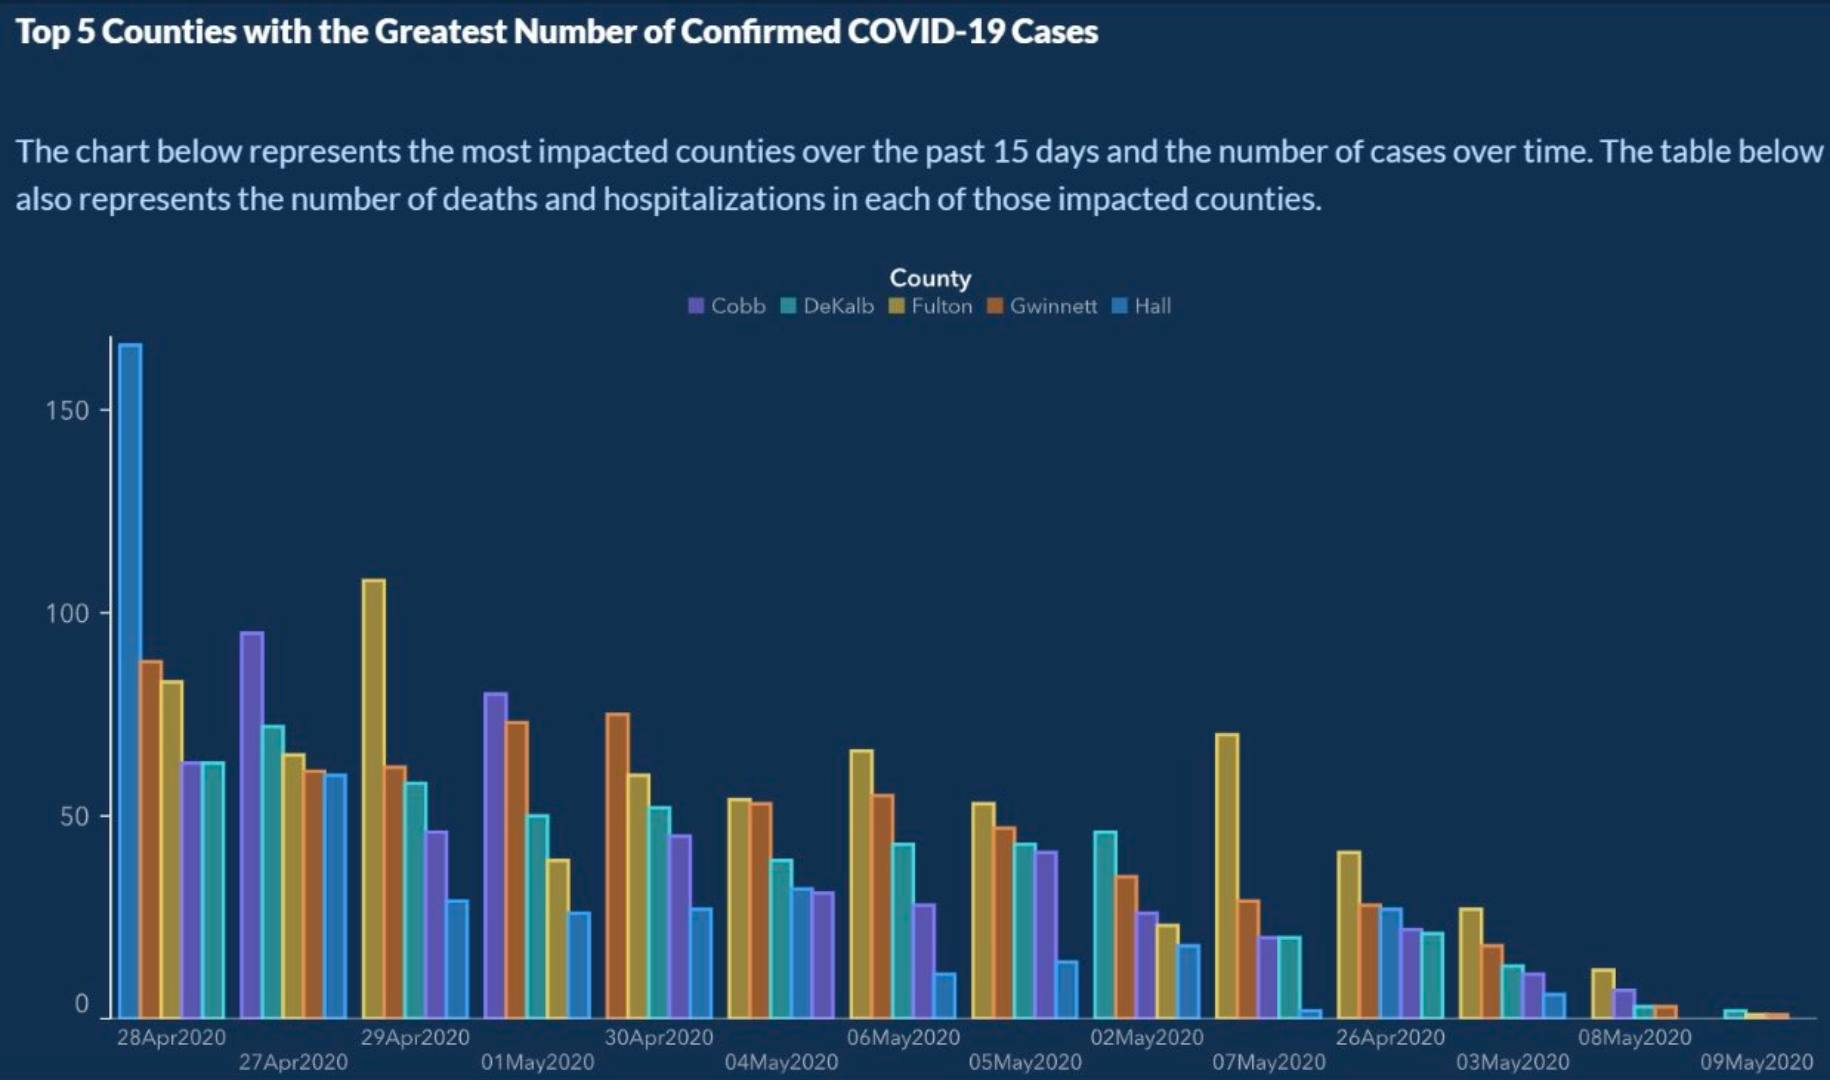
\includegraphics[width=25.42in]{images/04_datavis/georgia_covid} 

}

\caption{US State of Georgia, COVID-19 Deaths,
Source: https://ftalphaville.ft.com/2020/05/18/1589795135000/When-axes-get-truly-evil/}\label{fig:unnamed-chunk-64}
\end{figure}

There is an \href{https://ftalphaville.ft.com/2020/05/18/1589795135000/When-axes-get-truly-evil/}{excellents article} from the Financial Times about this chart. I think this chart is a great example of why data visualisation is important.

We use charts to communicate large amounts of data quickly and easily.

Often, in life, we are trying to communicate something important. We are often trying to persuade someone to do something, like give us more research money, or to make a change that we want to see.

What message do you think \textbf{Figure 4.1} is trying to communicate?

If you look at the x axis (the one that goes across the graph), what order are the dates in?

\hypertarget{vis_anatomy}{%
\subsection{Chart anatomy}\label{vis_anatomy}}

\hypertarget{the-two-axes-rule}{%
\subsubsection{The two-axes rule}\label{the-two-axes-rule}}

Most charts will have two axes:

\begin{itemize}
\item
  The \textbf{x axis} which goes \textbf{across the chart}
\item
  The \textbf{y axis} which goes \textbf{up the chart} (upp-\textbf{y}/down-\textbf{y} was how I used to remember it).
\end{itemize}

As in data science we are often interested in \textbf{does x affect y}, we usually put the \textbf{explanatory} variable on the x axis. We try to always have the thing that drives variation going across the chart, whereas the thing that responds to variation goes up and down the chart. (The response-\textbf{y} variable.)

You should always thing about your axes - and they should be clear to the reader from the beginning. No messing with the order (see again \textbf{Figure 4.1}).

Unless you have a very good reason, I would always have two axes. That means if you're trying to put in a second Y axis, you are breaking the two-axes rule, and should re-evaluate your chart. If you're trying to make a pie-chart, you are breaking the two-axes rule, and should re-evaluate your chart.

Follow the two-axes rule, and your life will be a lot easier.

\hypertarget{why-i-hate-pie-charts}{%
\subsubsection{Why I hate pie charts}\label{why-i-hate-pie-charts}}

Pie charts are the worst visualisation in the world.

\begin{figure}
\centering
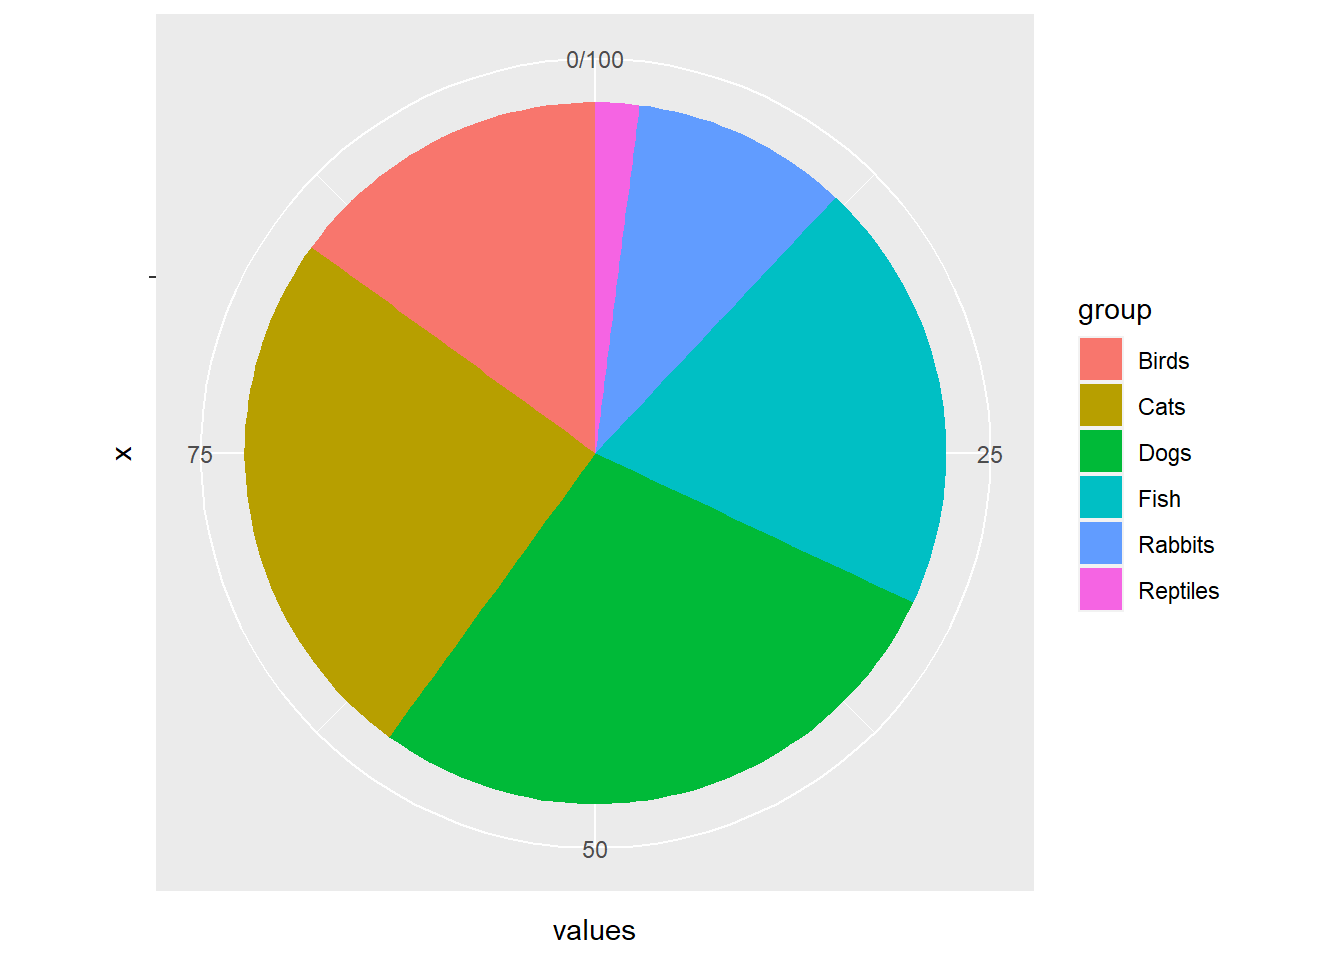
\includegraphics{ratrdsvs_files/figure-latex/unnamed-chunk-65-1.pdf}
\caption{\label{fig:unnamed-chunk-65}The worst kind of chart describing proportion of people with type of pet (fictional data)}
\end{figure}

Let's take \textbf{Figure 4.2} as an example. What proportion of people have a dog versus a cat. I'll wait for you to start puzzling through that question.

It's very hard to distinguish between a pie slice that's 2/5ths versus a pie slice that's 2/7ths. Many people put labels on their pie charts, but if I need to read the label to understand the difference, why not just put the text in a table?

Instead a bar chart shows use the exact ranking of this data and we can see how many more people have cats versus birds.

\begin{figure}
\centering
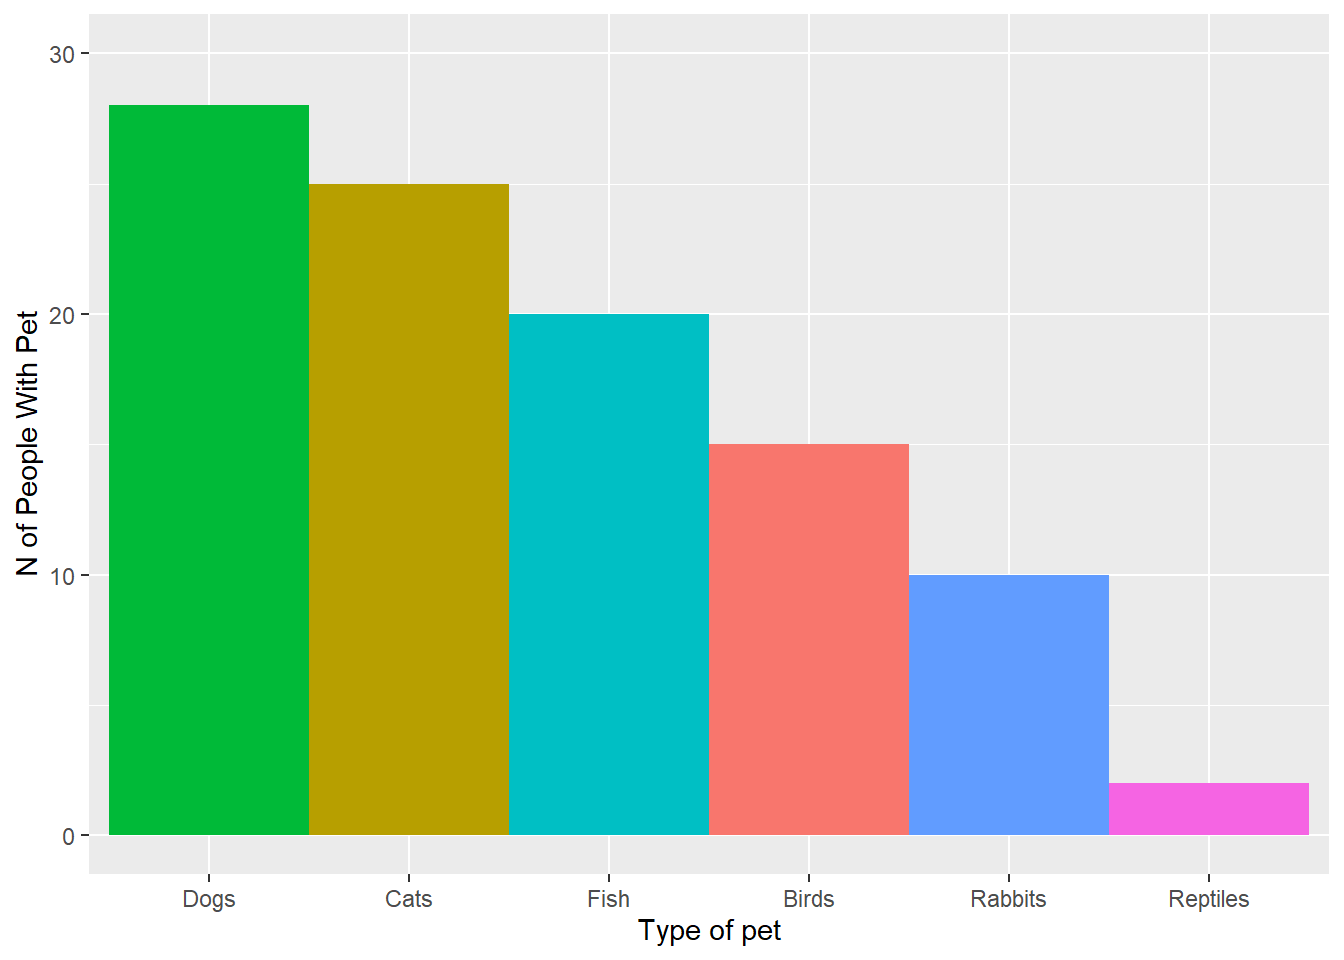
\includegraphics{ratrdsvs_files/figure-latex/unnamed-chunk-66-1.pdf}
\caption{\label{fig:unnamed-chunk-66}A much better chart describing proportion of people with type of pet (fictional data)}
\end{figure}

\hypertarget{figure-headings}{%
\subsubsection{Figure headings}\label{figure-headings}}

Figure headings should be a clear description of what is in the chart.

\hypertarget{legends}{%
\subsubsection{Legends}\label{legends}}

Like figure headings, legends should be informative and clear. They will always describe a categorical variable, and sometimes their job will be done by the x axis.

\hypertarget{colours}{%
\subsubsection{Colours}\label{colours}}

The use of colours in charts is a curious thing. Colour can be very useful in a chart, but also very distracting. There's another \href{https://www.ft.com/content/c4b7d8be-2eb0-11e8-9b4b-bc4b9f08f381}{brilliant FT article on the use of colour to indicate gender in charts} and all the ensuing complications.

\hypertarget{advanced-r-users}{%
\paragraph{Advanced R users}\label{advanced-r-users}}

If you have gotten really into R, or you really like pretty colours, I highly recommend checking out \href{https://github.com/EmilHvitfeldt/r-color-palettes}{Emil Hvitfeldt's well maintained repository} listing all the R colour palette packages out there. Personally I really like \texttt{nord}\footnote{I like \texttt{nord} so much its the colour scheme for this book} and \texttt{LaCroixColoR} and \texttt{NineteenEightyR}. Much of my life is spent tweaking colours on charts.

\hypertarget{vis_bar}{%
\subsection{Bar charts}\label{vis_bar}}

Bar charts are good for describing a continuous (numerical) variable by a categorical (grouping) variable. The continuous variable is often the average of a group. For example:

\begin{figure}
\centering
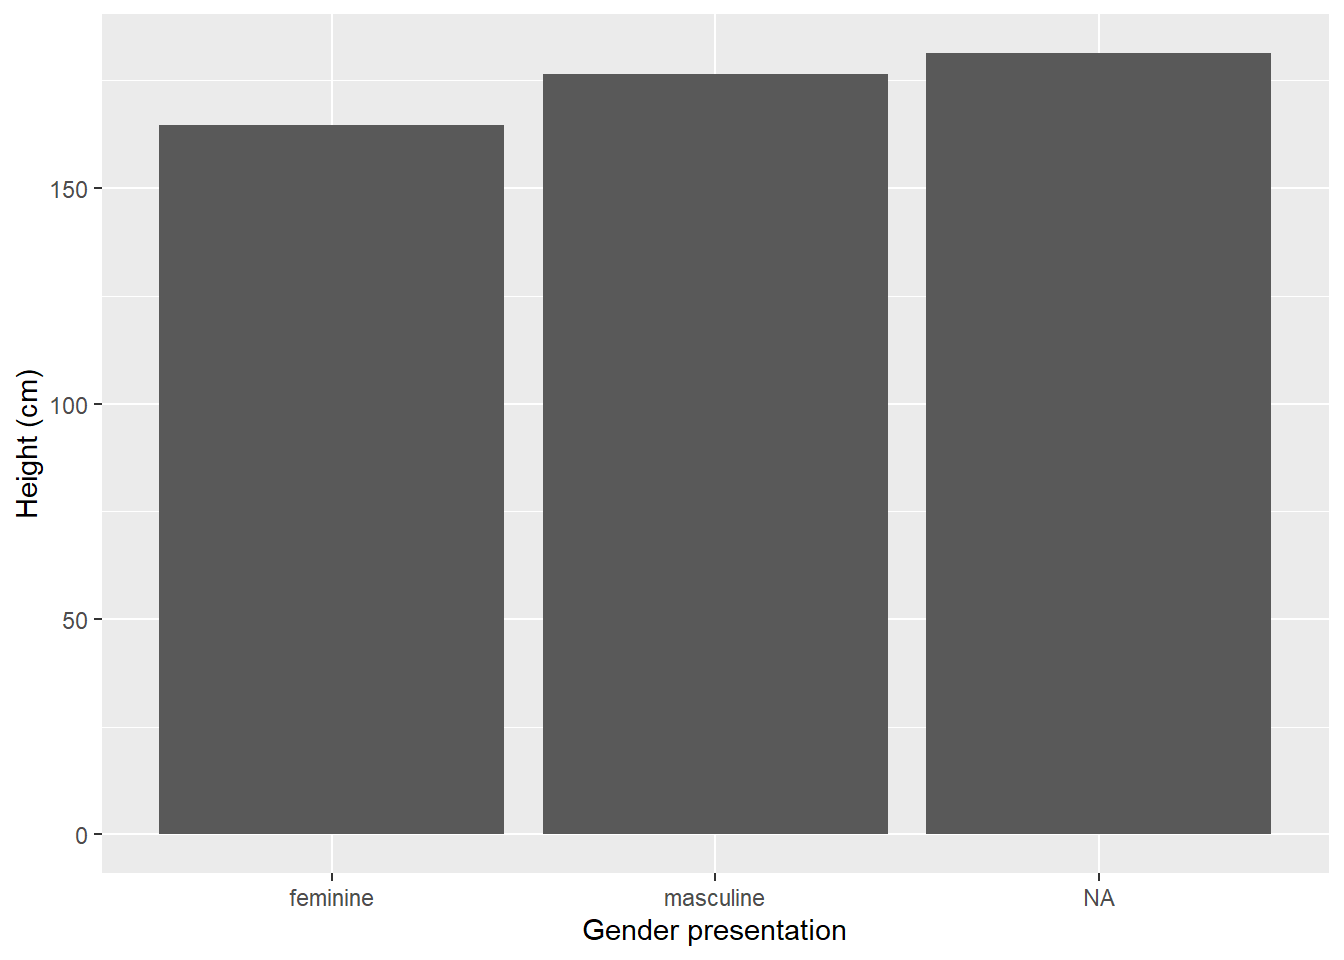
\includegraphics{ratrdsvs_files/figure-latex/unnamed-chunk-67-1.pdf}
\caption{\label{fig:unnamed-chunk-67}Averge height (cm) of Star Wars characters by gender}
\end{figure}

They can also be flipped around, particularly if the axis text is hard to read in one particular direction:

\begin{figure}
\centering
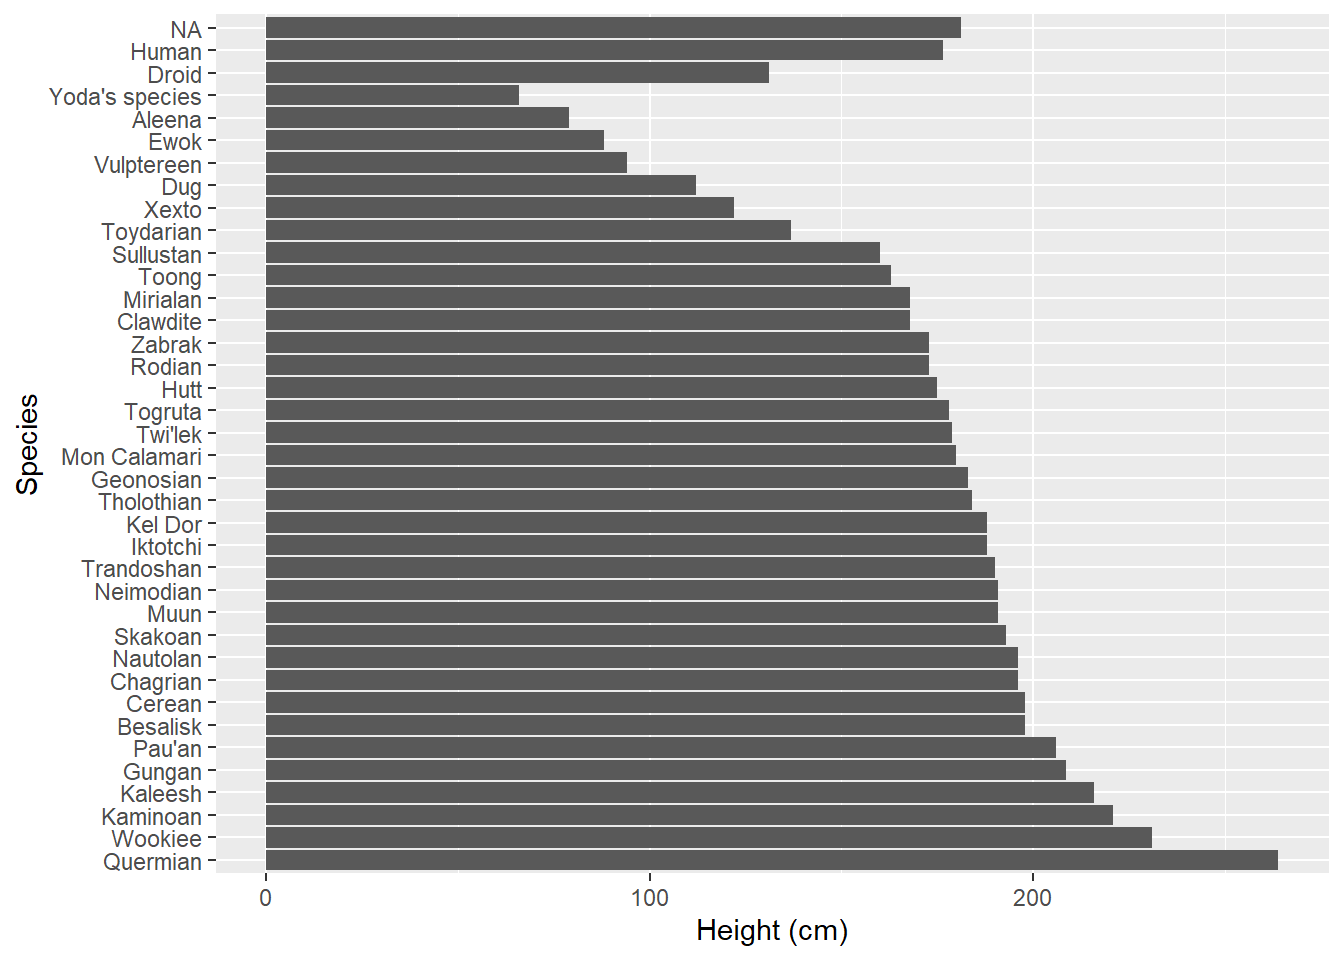
\includegraphics{ratrdsvs_files/figure-latex/unnamed-chunk-68-1.pdf}
\caption{\label{fig:unnamed-chunk-68}Averge height (cm) of Star Wars characters by species}
\end{figure}

\hypertarget{vis_hist}{%
\subsection{Histograms}\label{vis_hist}}

A histogram shows the relative frequency of a continuous variable. For example we can see the most common height of Star Wars characters, with 20 characters, is around 180cm:

\begin{figure}
\centering
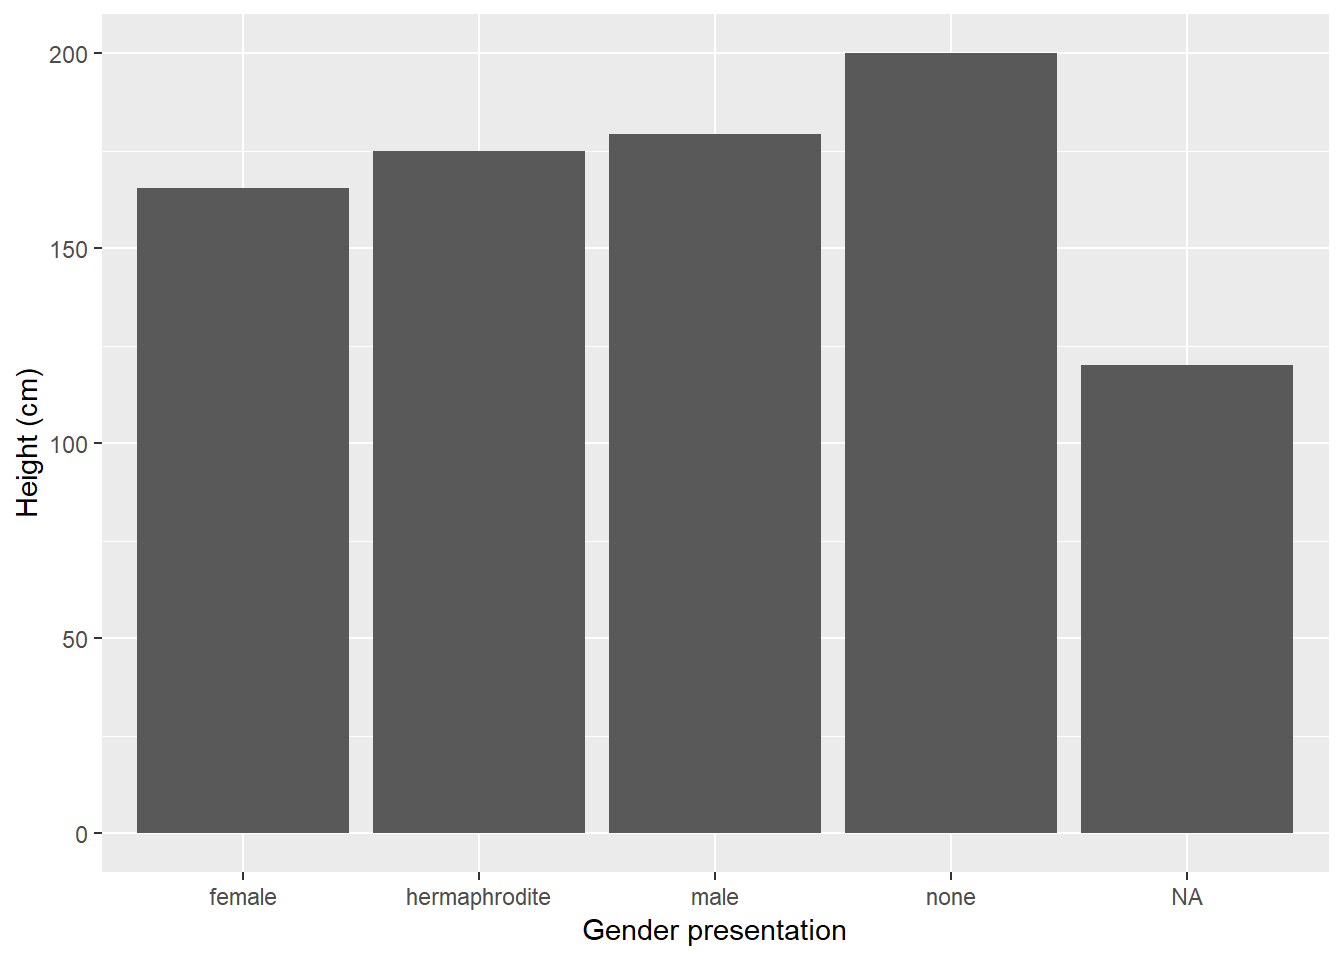
\includegraphics{ratrdsvs_files/figure-latex/unnamed-chunk-69-1.pdf}
\caption{\label{fig:unnamed-chunk-69}Histogram of height (cm) of Star Wars characters}
\end{figure}

\hypertarget{vis_scatter}{%
\subsection{Scatterplots}\label{vis_scatter}}

Scatterplots are good for showing the relationship between two continuous variables.

\begin{figure}
\centering
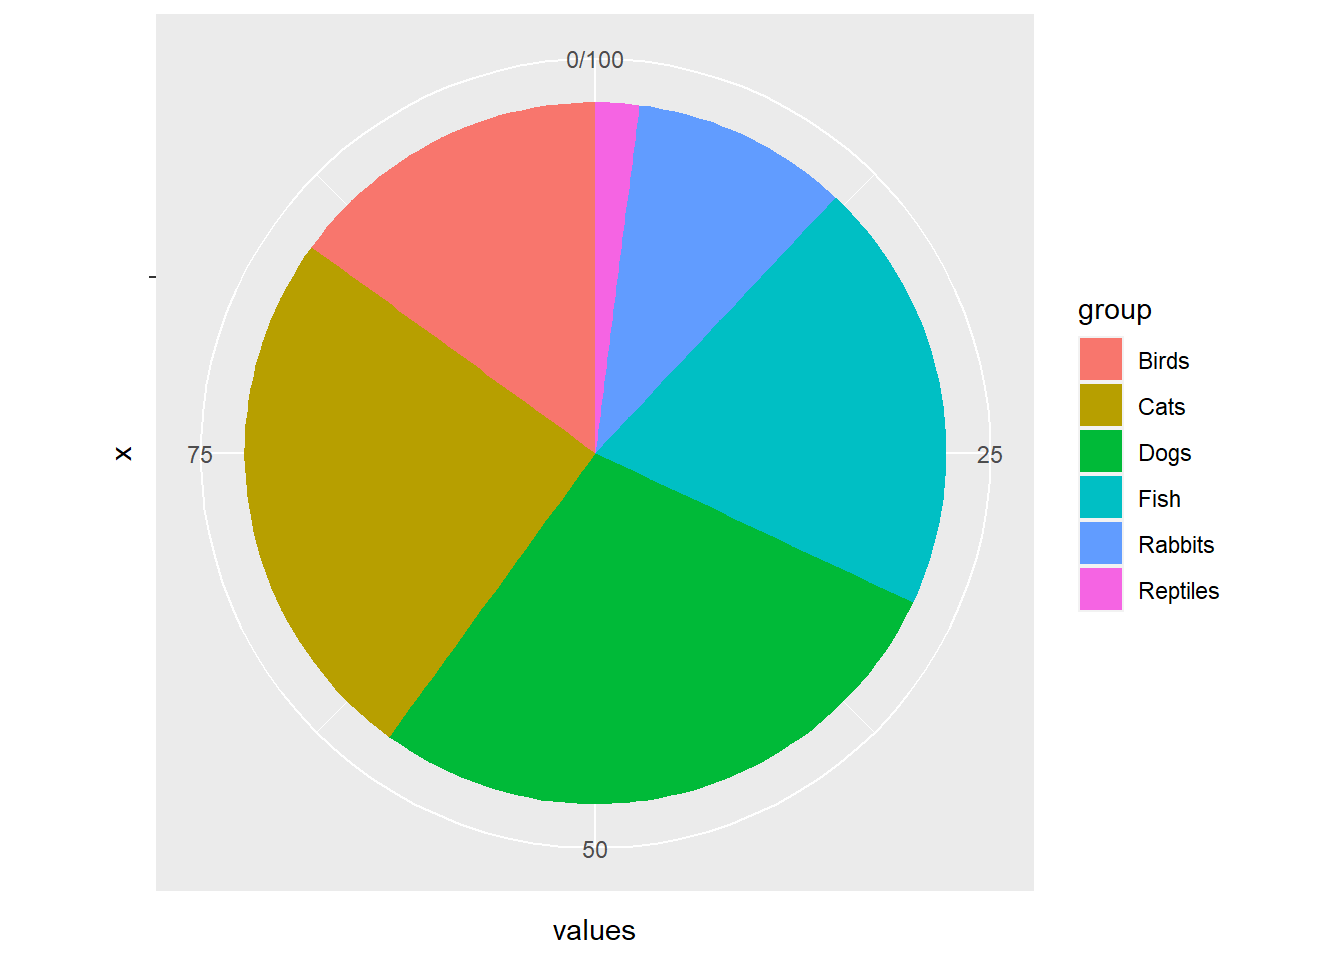
\includegraphics{ratrdsvs_files/figure-latex/unnamed-chunk-70-1.pdf}
\caption{\label{fig:unnamed-chunk-70}Averge height (cm) of Star Wars characters by weight (kg)}
\end{figure}

But we can use other aspects, such as shape or colour, to add in a categorical variable:

\begin{figure}
\centering
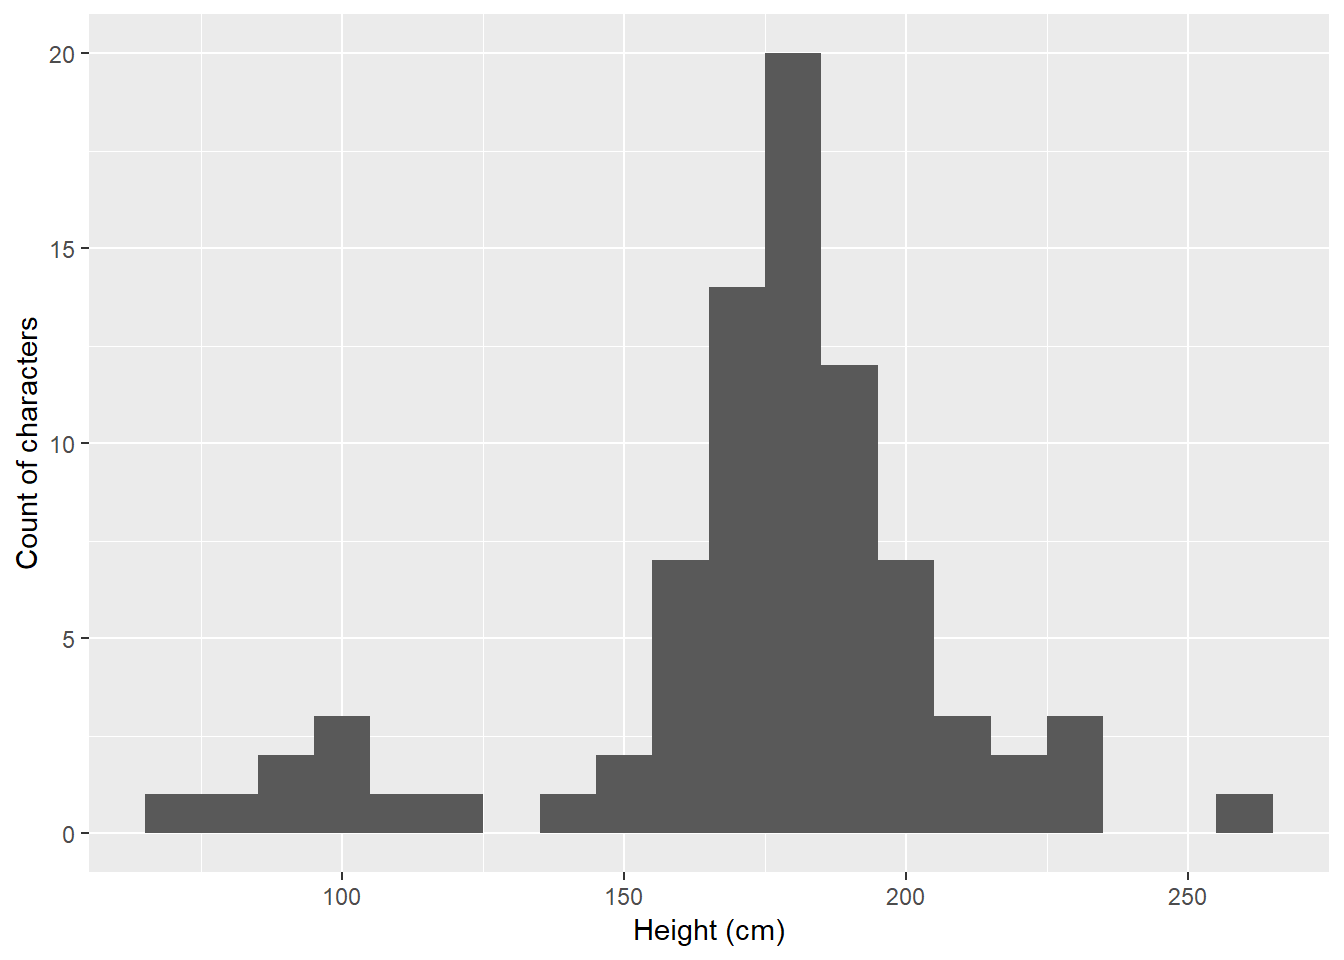
\includegraphics{ratrdsvs_files/figure-latex/unnamed-chunk-71-1.pdf}
\caption{\label{fig:unnamed-chunk-71}Averge height (cm) of Star Wars characters by weight (kg) and species}
\end{figure}

\hypertarget{vis_box}{%
\subsection{Boxplots}\label{vis_box}}

Boxplots are another way to examine a continuous variable by a categorical variable, but they give us a lot more information than a bar plot does.

A boxplot shows you:

\begin{itemize}
\item
  The \textbf{median} value (the thick bar in the middle)
\item
  The \textbf{first quartile} (the lowest part of the bar)
\item
  The \textbf{third quartile} (the highest part of the bar)
\item
  A \textbf{lower hinge} (the bottom thin line) which roughly equates to 95\% of the data will not be below this value.
\item
  An \textbf{upper hinge} (the top thin line) which roughy equates to 95\% of the data will not be above this value.
\item
  Any \textbf{outliers} (the dots) which are observations which lie outside of 95\% of the data\footnote{The hinges are actually calculated based on the \texttt{boxplot.stats} \href{https://www.rdocumentation.org/packages/grDevices/versions/3.6.2/topics/boxplot.stats}{function} which is a little more complicated than 95\% of the data - but if you ever need to worry about this you have gone beyond what this book can teach you.}
\end{itemize}

\begin{figure}
\centering
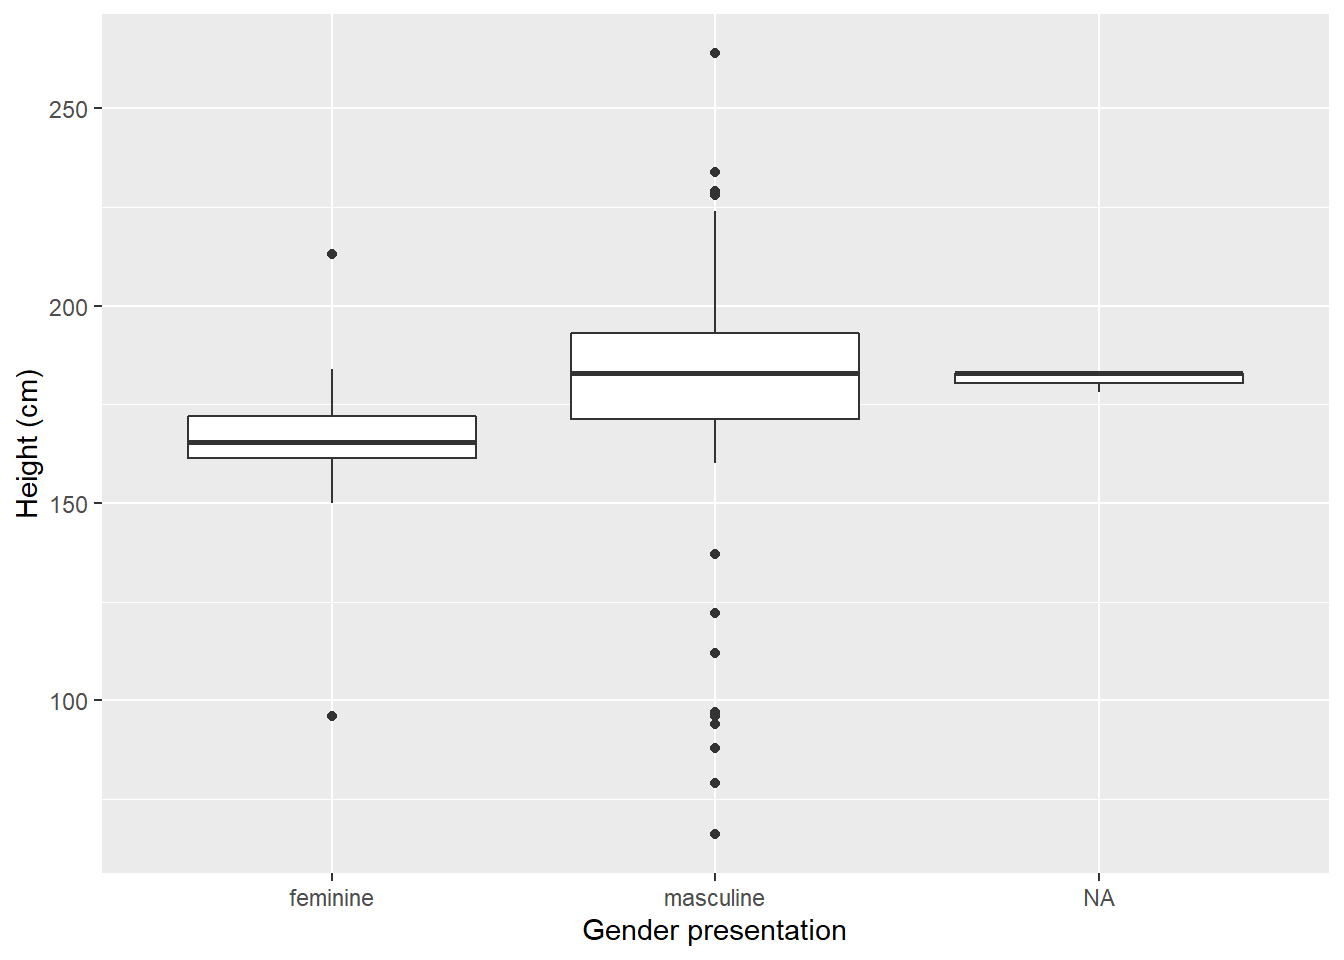
\includegraphics{ratrdsvs_files/figure-latex/unnamed-chunk-72-1.pdf}
\caption{\label{fig:unnamed-chunk-72}Averge height (cm) of Star Wars characters by gender}
\end{figure}

\hypertarget{vis_infographic}{%
\subsection{Infographics}\label{vis_infographic}}

In our increasingly connected world, we are seeing more and more infographics. As they're less standardised, there can be more room for interpretation. For example;

As an Indian woman, I can confirm that too much of my time is spent hiding behind a rock praying the terrifying gang of international giant ladies and their Latvian general don't find me pic.twitter.com/sy9NHW9oTK

--- Sabah Ibrahim (@reina\_sabah) August 6, 2020

Infographics can be extremely powerful, particularly when trying to communicate on social media. Unfortunately, sometimes the design choices can make it harder to understand exactly what the analysis has done. Infographics can be as misleading as bad charts.

In general, I would focus on chart visualisations over infographics, even for public engagement. When you are very confident with making clear and readable charts, then you can start to think about infographics.

\hypertarget{ggplot}{%
\chapter{ggplot2}\label{ggplot}}

\begin{los}
You can skip this chapter if:

\begin{itemize}
\item
  You are confident using the \texttt{ggplot2} package
\item
  You can use the \texttt{geom\_bar}, \texttt{geom\_point} and
  \texttt{geom\_histogram} arguments
\item
  You can customise a ggplot2 object
\end{itemize}
\end{los}

\hypertarget{why-ggplot}{%
\section{Why ggplot?}\label{why-ggplot}}

There is a fierce debate in the land of R. Some people think basic R shoud be taught first. Others think that you should learn how to do more complicated things first.

I think you should start to learn ggplot2.

ggplot2 is a really great way to learn R, and particularly the \texttt{tidyverse} approach to coding. It also makes beautiful charts. All my charts in the last chapter (even the dreaded pie chart) were made in ggplot2.

\hypertarget{gg_build}{%
\section{Building a ggplot object (a scatterplot)}\label{gg_build}}

First - open an R Script or RMD file and load the \texttt{tidyverse} package:

\begin{Shaded}
\begin{Highlighting}[]
\KeywordTok{library}\NormalTok{(tidyverse)}
\end{Highlighting}
\end{Shaded}

Let's choose the \texttt{diamonds} dataset (from \texttt{ggplot2} - you can check this by running \texttt{?diamonds}), and take a look.

\begin{Shaded}
\begin{Highlighting}[]
\KeywordTok{head}\NormalTok{(diamonds)}
\end{Highlighting}
\end{Shaded}

\begin{verbatim}
## # A tibble: 6 x 10
##   carat cut       color clarity depth table price     x     y     z
##   <dbl> <ord>     <ord> <ord>   <dbl> <dbl> <int> <dbl> <dbl> <dbl>
## 1 0.23  Ideal     E     SI2      61.5    55   326  3.95  3.98  2.43
## 2 0.21  Premium   E     SI1      59.8    61   326  3.89  3.84  2.31
## 3 0.23  Good      E     VS1      56.9    65   327  4.05  4.07  2.31
## 4 0.290 Premium   I     VS2      62.4    58   334  4.2   4.23  2.63
## 5 0.31  Good      J     SI2      63.3    58   335  4.34  4.35  2.75
## 6 0.24  Very Good J     VVS2     62.8    57   336  3.94  3.96  2.48
\end{verbatim}

\begin{translate}
We want to take the \texttt{diamonds} dataset and then
(\texttt{\%\textgreater{}\%}) send it to \texttt{ggplot}.

In \texttt{ggplot} we will use the \textbf{aesthetics} argument
(\texttt{aes}) to tell R what to put on the \texttt{x} axis and the
\texttt{y} axis.
\end{translate}

\begin{Shaded}
\begin{Highlighting}[]
\NormalTok{diamonds }\OperatorTok\StringTok{ }
\StringTok{  }\KeywordTok{ggplot}\NormalTok{(}\KeywordTok{aes}\NormalTok{(}\DataTypeTok{x =}\NormalTok{ carat, }\DataTypeTok{y =}\NormalTok{ price))}
\end{Highlighting}
\end{Shaded}

What do you think this code will do?

\textbf{Try this code first!}

This code ends up giving us a blank chart. This seems strange until you figure out that ggplot works by \textbf{layering} elements of a chart on top of one another:

\begin{Shaded}
\begin{Highlighting}[]
\NormalTok{diamonds }\OperatorTok\StringTok{ }
\StringTok{  }\KeywordTok{ggplot}\NormalTok{(}\KeywordTok{aes}\NormalTok{(}\DataTypeTok{x =}\NormalTok{ carat, }\DataTypeTok{y =}\NormalTok{ price))}
\end{Highlighting}
\end{Shaded}

\begin{figure}
\centering
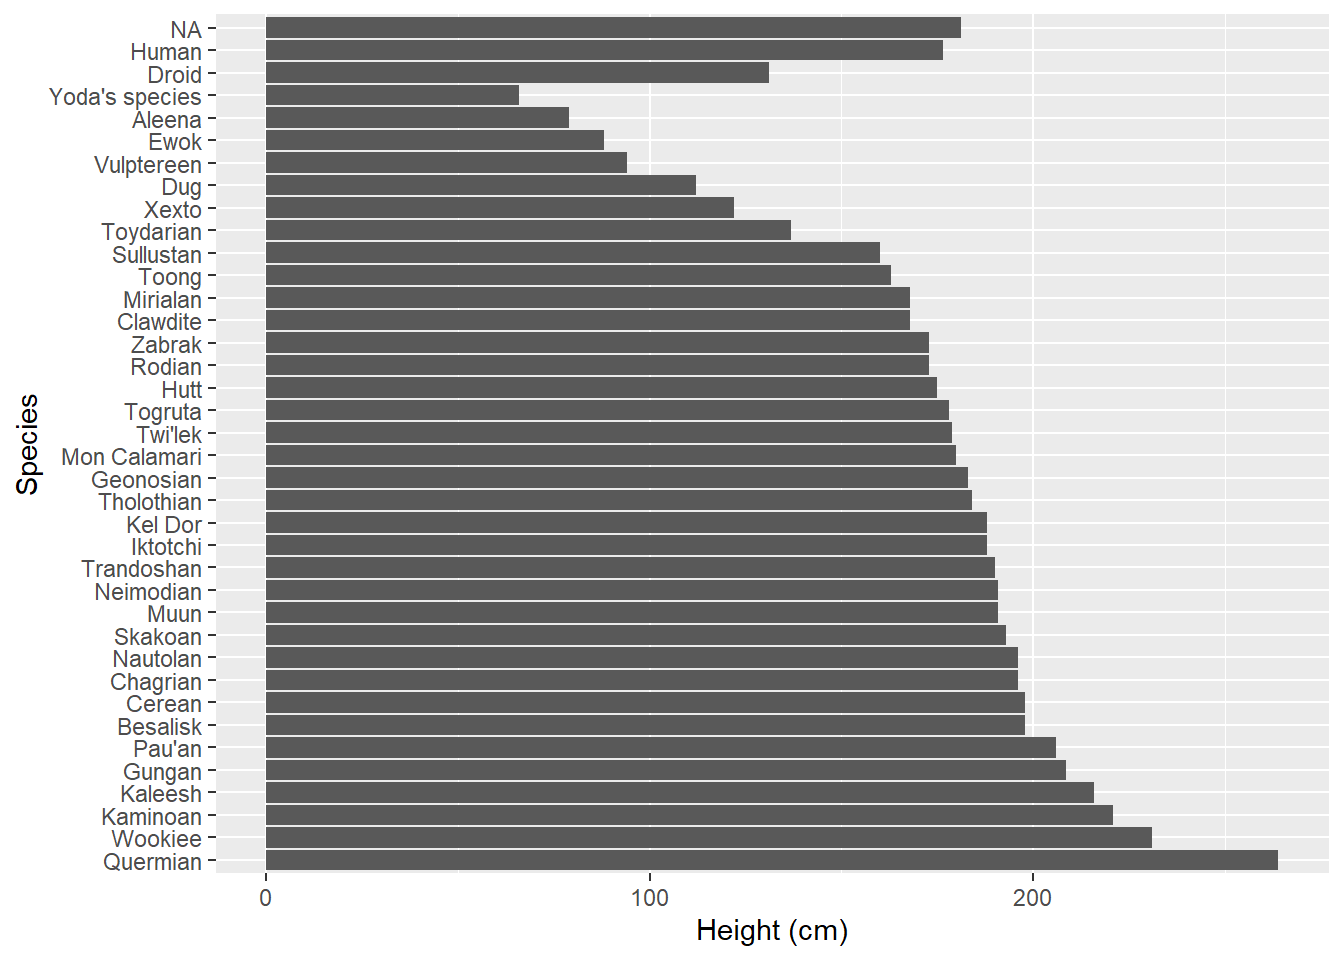
\includegraphics{ratrdsvs_files/figure-latex/unnamed-chunk-78-1.pdf}
\caption{\label{fig:unnamed-chunk-78}A ggplot object with no geom layers}
\end{figure}

We need to tell R to add a \texttt{geom} layer, and we do that by adding a \texttt{+}\footnote{You may be interested to know that the \texttt{+} symbol is a precursor to the \texttt{\%\textgreater{}\%} symbol. Both \texttt{ggplot2} and \texttt{tidyverse} were mainly written by \href{https://twitter.com/hadleywickham}{Hadley Wickham} who has often spoken about \href{https://community.rstudio.com/t/why-cant-ggplot2-use/4372/7}{why ggplot won't ever use the \%\textgreater{}\% operator}} symbol. In this case, we want to add a \texttt{geom\_point} layer, so we write the following:

\begin{Shaded}
\begin{Highlighting}[]
\NormalTok{diamonds }\OperatorTok\StringTok{ }
\StringTok{  }\KeywordTok{ggplot}\NormalTok{(}\KeywordTok{aes}\NormalTok{(}\DataTypeTok{x =}\NormalTok{ carat, }\DataTypeTok{y =}\NormalTok{ price)) }\OperatorTok{+}\StringTok{ }
\StringTok{  }\KeywordTok{geom_point}\NormalTok{()}
\end{Highlighting}
\end{Shaded}

\begin{figure}
\centering
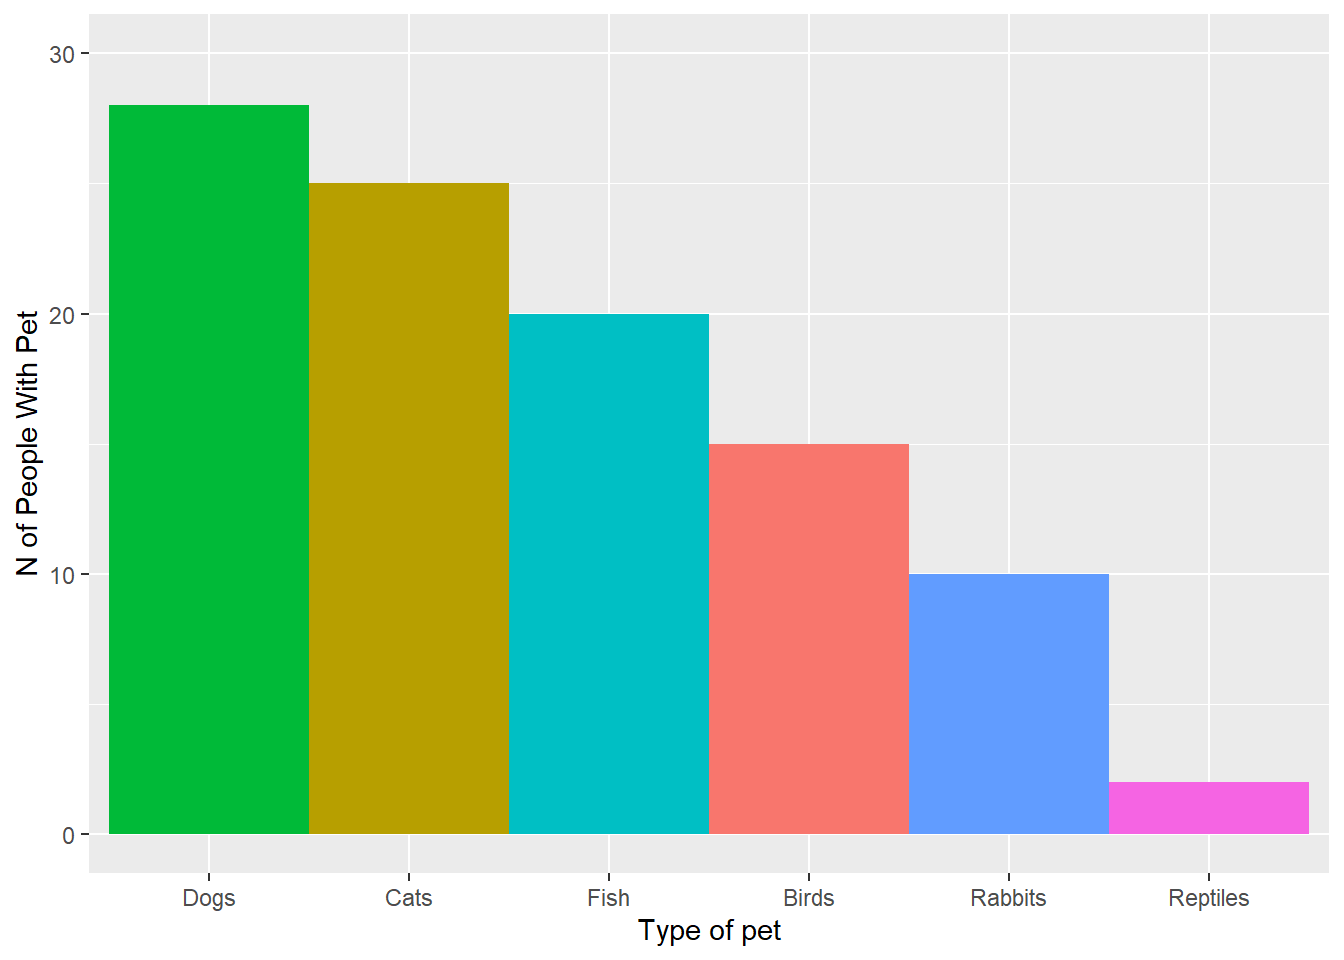
\includegraphics{ratrdsvs_files/figure-latex/unnamed-chunk-79-1.pdf}
\caption{\label{fig:unnamed-chunk-79}A ggplot object with a geom\_point layer, the price of diamonds by their carat}
\end{figure}

Look at how quickly and easily that worked. With three lines of code, you created a chart of 50,000 datapoints.

That must make you wonder what else you can do . . .

\hypertarget{gg_axis}{%
\subsection{Changing an axis in ggplot2}\label{gg_axis}}

Let's change the x axis on this chart. At the moment, we have a `tick' mark at every carat, but what if we want to have a `tick' mark at every 0.5 carats?

All we need is another line of code.

\begin{Shaded}
\begin{Highlighting}[]
\NormalTok{diamonds }\OperatorTok\StringTok{ }
\StringTok{  }\KeywordTok{ggplot}\NormalTok{(}\KeywordTok{aes}\NormalTok{(}\DataTypeTok{x =}\NormalTok{ carat, }\DataTypeTok{y =}\NormalTok{ price)) }\OperatorTok{+}\StringTok{ }
\StringTok{  }\KeywordTok{geom_point}\NormalTok{() }\OperatorTok{+}
\StringTok{  }\KeywordTok{scale_x_continuous}\NormalTok{(}\DataTypeTok{breaks =} \KeywordTok{seq}\NormalTok{ (}\DecValTok{0}\NormalTok{, }\DecValTok{5}\NormalTok{, }\FloatTok{0.5}\NormalTok{))}
\end{Highlighting}
\end{Shaded}

\begin{figure}
\centering
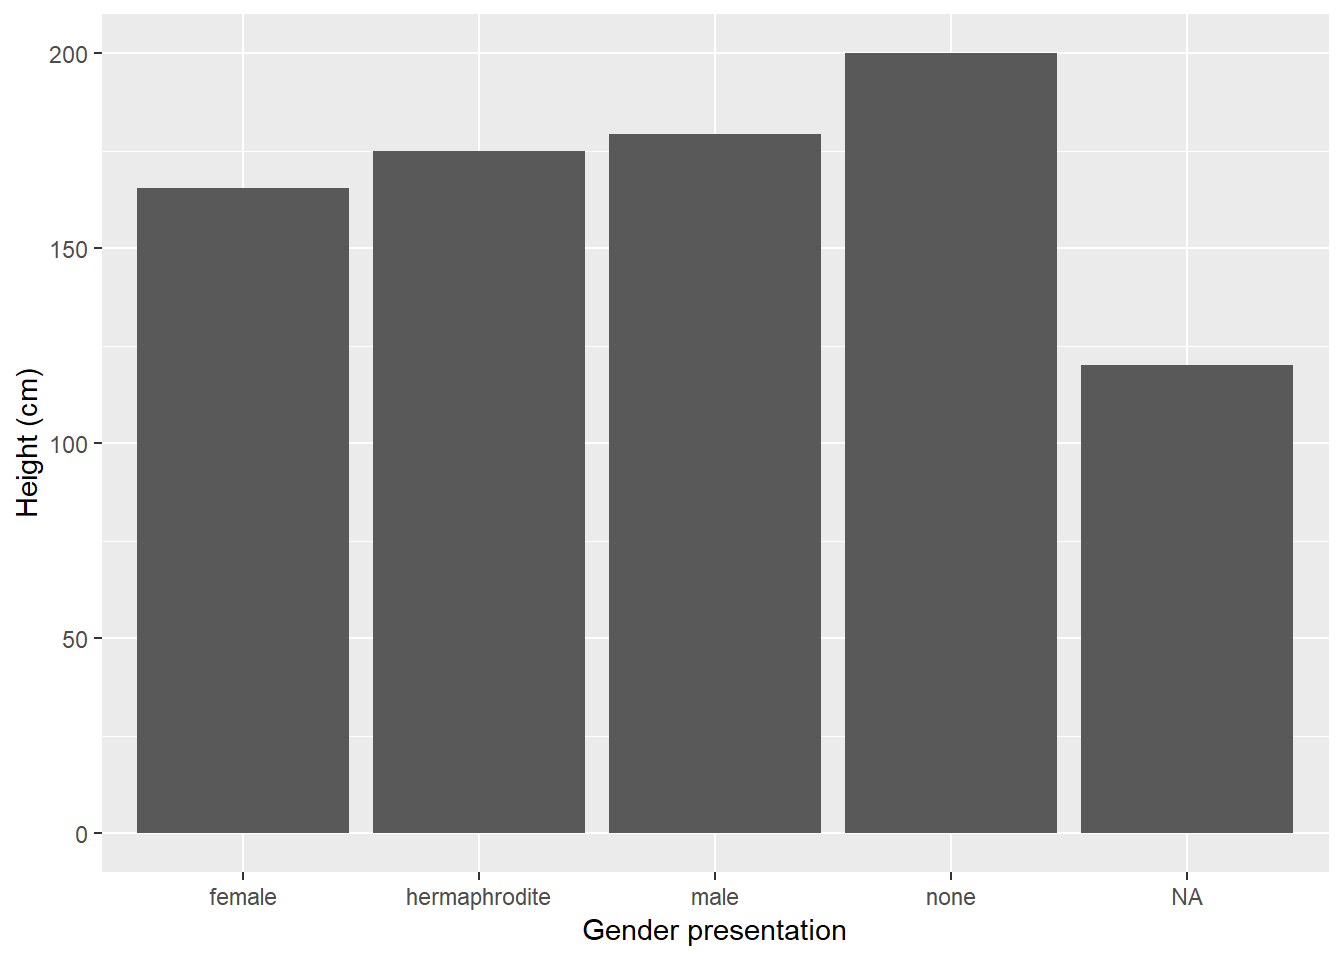
\includegraphics{ratrdsvs_files/figure-latex/unnamed-chunk-80-1.pdf}
\caption{\label{fig:unnamed-chunk-80}A ggplot object with a geom\_point layer, the price of diamonds by their carat, x axis changed}
\end{figure}

The \texttt{scale\_x\_continuous} line reads:

\begin{translate}
Take the last three lines of code and then (\texttt{+})

\begin{itemize}
\item
  Change the scale of the x axis (\texttt{scale\_x\_}) which is a
  continuous (\texttt{scale\_x\_continuous}) variable.
\item
  Change the numbers along the axis (\texttt{breaks\ =}) to a sequence
  (\texttt{seq})
\item
  The sequence starts at \texttt{0}, goes to \texttt{5}, and the spaces
  between them should be \texttt{0.5}
\end{itemize}
\end{translate}

We can go further by changing the limits within the\texttt{scale\_x\_} command \ldots{}

\begin{Shaded}
\begin{Highlighting}[]
\NormalTok{diamonds }\OperatorTok\StringTok{ }
\StringTok{  }\KeywordTok{ggplot}\NormalTok{(}\KeywordTok{aes}\NormalTok{(}\DataTypeTok{x =}\NormalTok{ carat, }\DataTypeTok{y =}\NormalTok{ price)) }\OperatorTok{+}\StringTok{ }
\StringTok{  }\KeywordTok{geom_point}\NormalTok{() }\OperatorTok{+}
\StringTok{  }\KeywordTok{scale_x_continuous}\NormalTok{(}\DataTypeTok{breaks =} \KeywordTok{seq}\NormalTok{ (}\DecValTok{0}\NormalTok{, }\DecValTok{5}\NormalTok{, }\FloatTok{0.5}\NormalTok{), }\DataTypeTok{limits =} \KeywordTok{c}\NormalTok{(}\DecValTok{0}\NormalTok{, }\DecValTok{6}\NormalTok{))}
\end{Highlighting}
\end{Shaded}

\begin{figure}
\centering
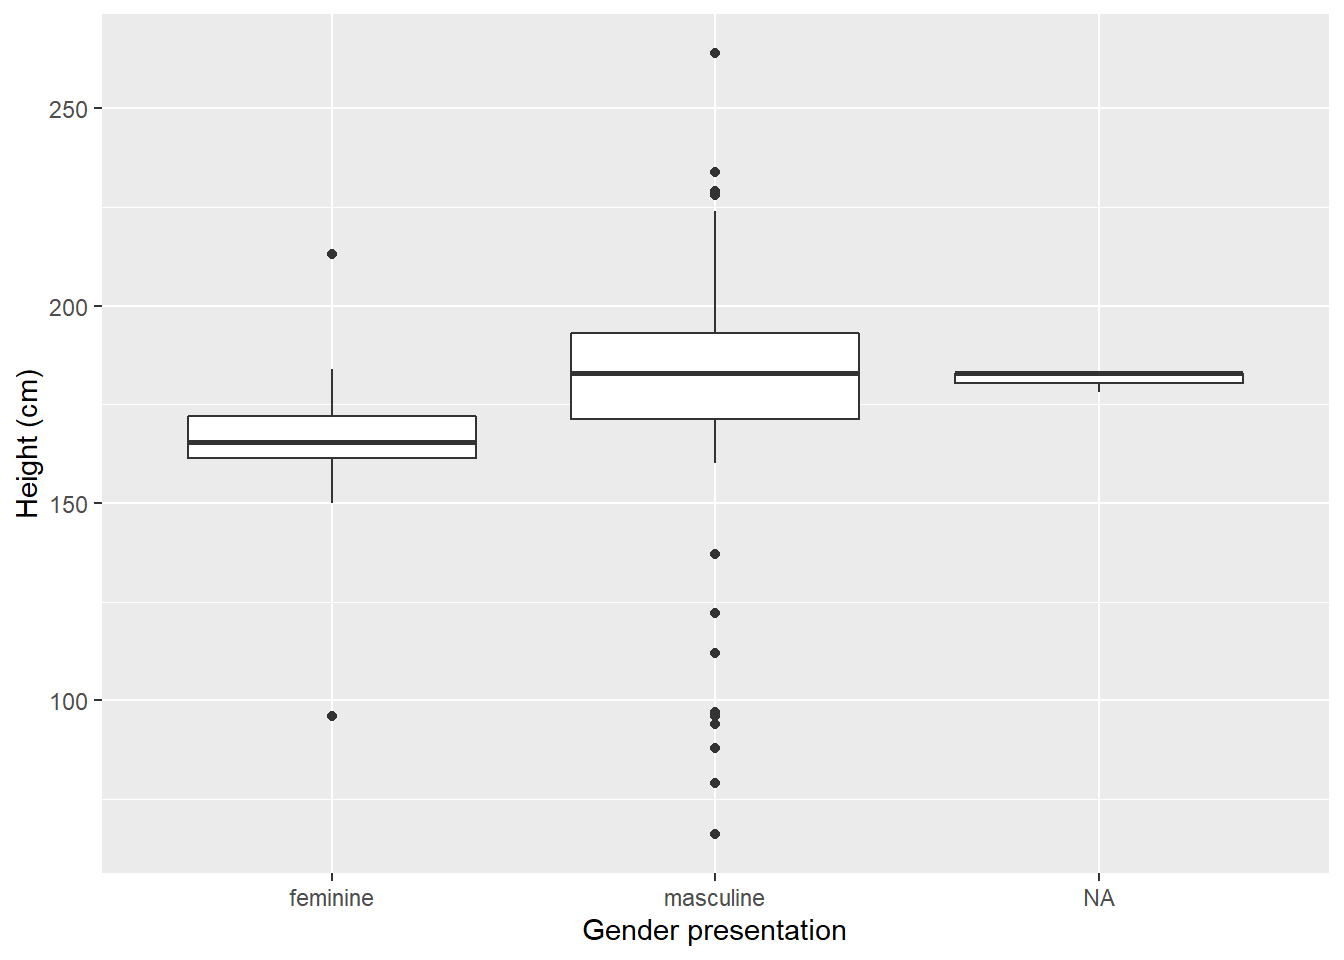
\includegraphics{ratrdsvs_files/figure-latex/unnamed-chunk-82-1.pdf}
\caption{\label{fig:unnamed-chunk-82}A ggplot object with a geom\_point layer, the price of diamonds by their carat, x axis changed}
\end{figure}

Now we've told R:

\begin{translate}
\begin{itemize}
\item
  Change the scale of x
\item
  Set new limits on x (\texttt{limits\ =})
\item
  The limits are a vector of two numbers together (\texttt{c()})
\item
  Start at \texttt{0} and end at \texttt{6}
\end{itemize}
\end{translate}

However, you'll notice that the numbers don't go all the way to the end. Have you spotted our mistake?

We need to change the \texttt{seq} command earlier in the argument\ldots{}

\begin{Shaded}
\begin{Highlighting}[]
\NormalTok{diamonds }\OperatorTok\StringTok{ }
\StringTok{  }\KeywordTok{ggplot}\NormalTok{(}\KeywordTok{aes}\NormalTok{(}\DataTypeTok{x =}\NormalTok{ carat, }\DataTypeTok{y =}\NormalTok{ price)) }\OperatorTok{+}\StringTok{ }
\StringTok{  }\KeywordTok{geom_point}\NormalTok{() }\OperatorTok{+}
\StringTok{  }\KeywordTok{scale_x_continuous}\NormalTok{(}\DataTypeTok{breaks =} \KeywordTok{seq}\NormalTok{ (}\DecValTok{0}\NormalTok{, }\DecValTok{6}\NormalTok{, }\FloatTok{0.5}\NormalTok{), }\DataTypeTok{limits =} \KeywordTok{c}\NormalTok{(}\DecValTok{0}\NormalTok{, }\DecValTok{6}\NormalTok{))}
\end{Highlighting}
\end{Shaded}

\begin{figure}
\centering
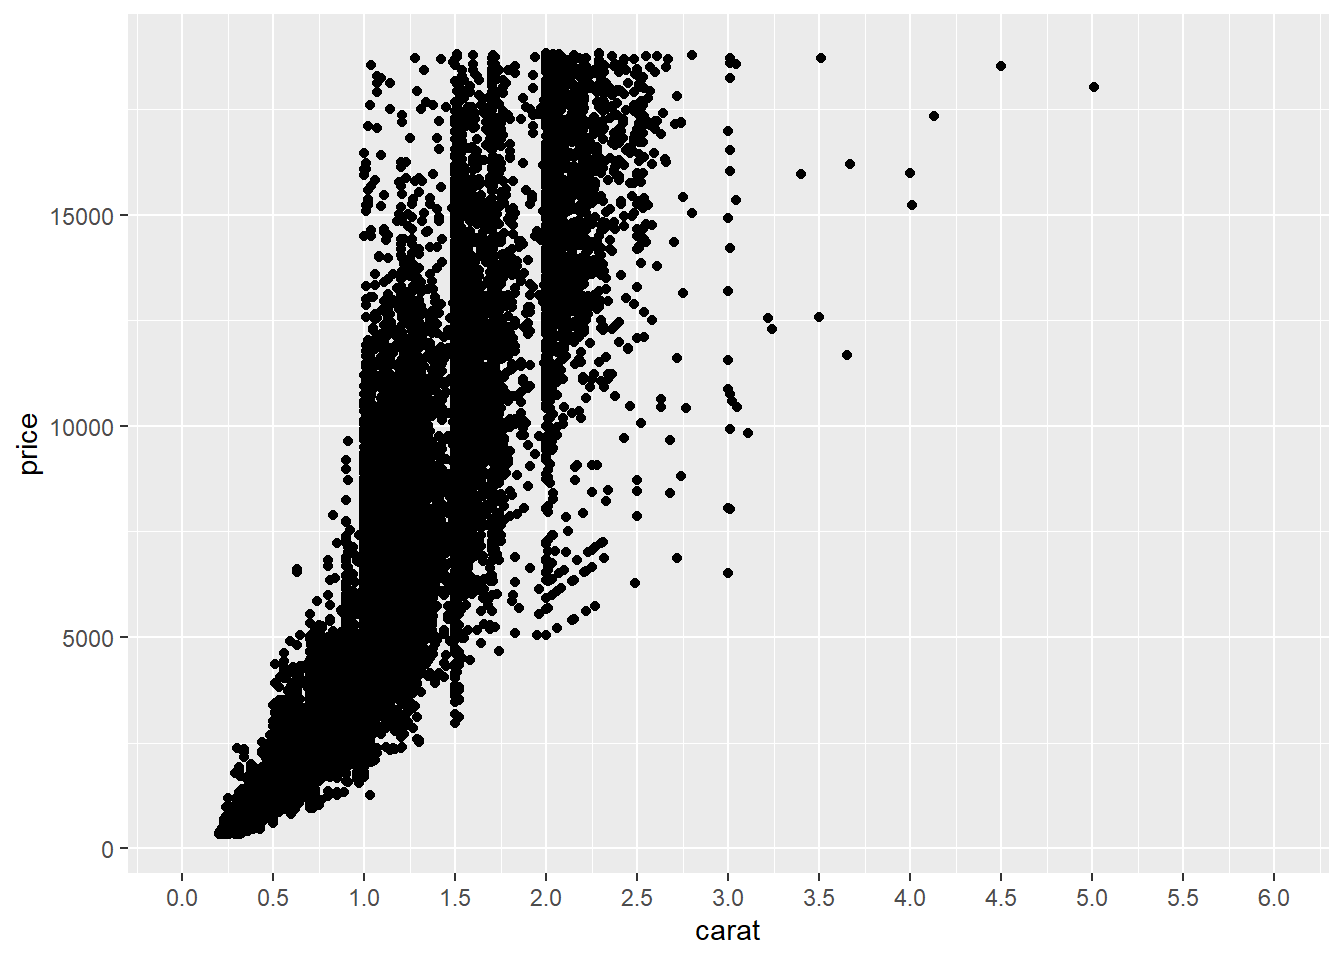
\includegraphics{ratrdsvs_files/figure-latex/unnamed-chunk-84-1.pdf}
\caption{\label{fig:unnamed-chunk-84}A ggplot object with a geom\_point layer, the price of diamonds by their carat, x axis changed}
\end{figure}

And we can change the y axis in much the same way:

\begin{Shaded}
\begin{Highlighting}[]
\NormalTok{diamonds }\OperatorTok\StringTok{ }
\StringTok{  }\KeywordTok{ggplot}\NormalTok{(}\KeywordTok{aes}\NormalTok{(}\DataTypeTok{x =}\NormalTok{ carat, }\DataTypeTok{y =}\NormalTok{ price)) }\OperatorTok{+}\StringTok{ }
\StringTok{  }\KeywordTok{geom_point}\NormalTok{() }\OperatorTok{+}
\StringTok{  }\KeywordTok{scale_x_continuous}\NormalTok{(}\DataTypeTok{breaks =} \KeywordTok{seq}\NormalTok{ (}\DecValTok{0}\NormalTok{, }\DecValTok{5}\NormalTok{, }\FloatTok{0.5}\NormalTok{), }\DataTypeTok{limits =} \KeywordTok{c}\NormalTok{(}\DecValTok{0}\NormalTok{, }\DecValTok{6}\NormalTok{)) }\OperatorTok{+}
\StringTok{  }\KeywordTok{scale_y_continuous}\NormalTok{(}\DataTypeTok{breaks =} \KeywordTok{seq}\NormalTok{(}\DecValTok{0}\NormalTok{, }\DecValTok{20000}\NormalTok{, }\DecValTok{2500}\NormalTok{), }\DataTypeTok{limits =} \KeywordTok{c}\NormalTok{(}\DecValTok{0}\NormalTok{, }\DecValTok{20000}\NormalTok{))}
\end{Highlighting}
\end{Shaded}

\begin{figure}
\centering
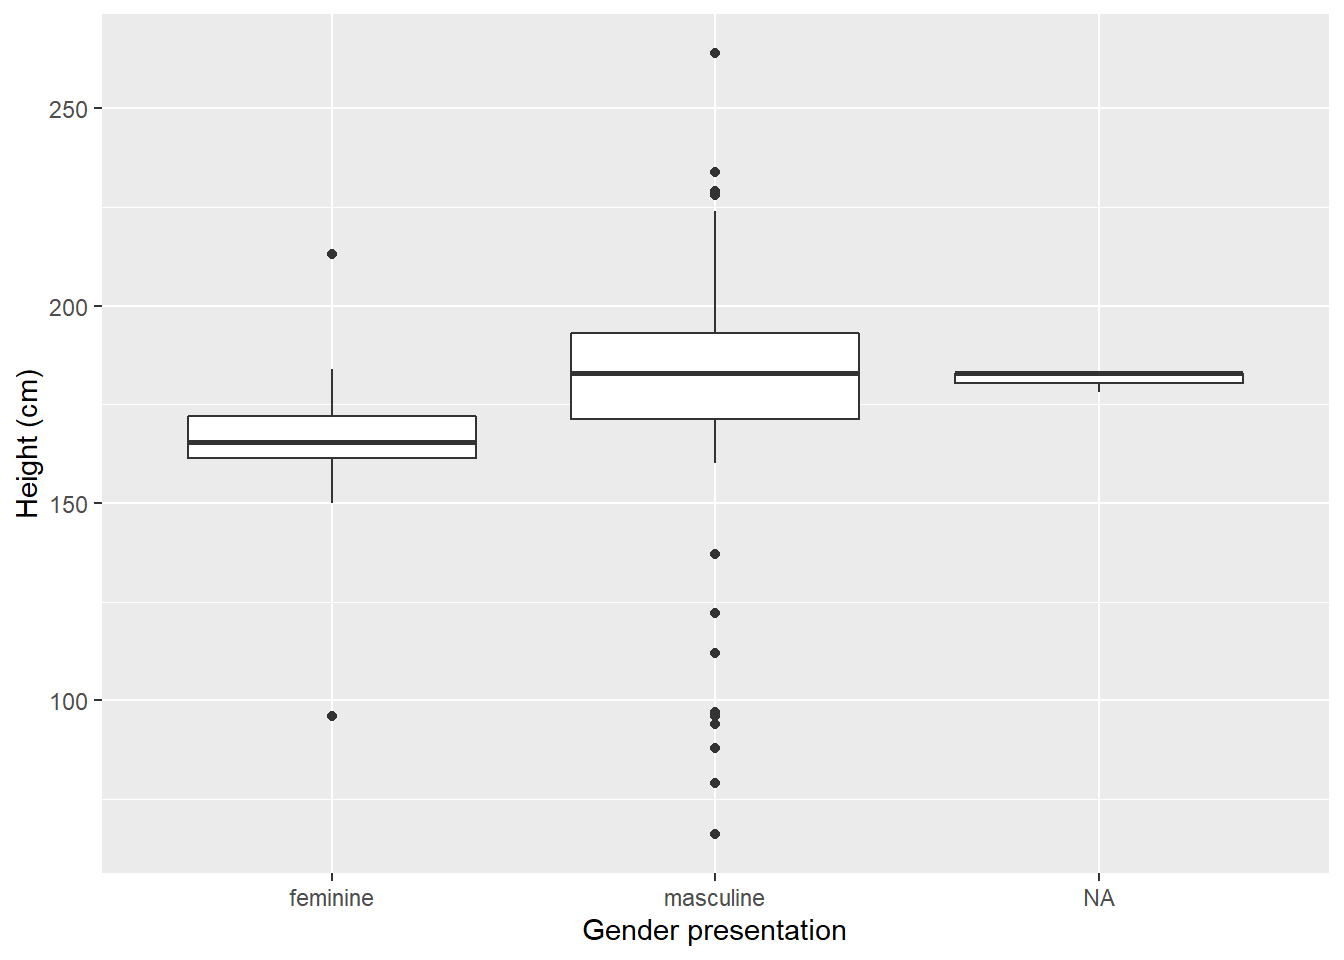
\includegraphics{ratrdsvs_files/figure-latex/unnamed-chunk-85-1.pdf}
\caption{\label{fig:unnamed-chunk-85}A ggplot object with a geom\_point layer, the price of diamonds by their carat, x and y axes changed}
\end{figure}

\hypertarget{gg_theme}{%
\subsection{Changing themes}\label{gg_theme}}

Themes are a very cool way to quickly change the look of and customise your charts. Just like everything else in ggplot, we just want to add another layer of code.

\begin{Shaded}
\begin{Highlighting}[]
\NormalTok{diamonds }\OperatorTok\StringTok{ }
\StringTok{  }\KeywordTok{ggplot}\NormalTok{(}\KeywordTok{aes}\NormalTok{(}\DataTypeTok{x =}\NormalTok{ carat, }\DataTypeTok{y =}\NormalTok{ price)) }\OperatorTok{+}\StringTok{ }
\StringTok{  }\KeywordTok{geom_point}\NormalTok{() }\OperatorTok{+}
\StringTok{  }\KeywordTok{scale_x_continuous}\NormalTok{(}\DataTypeTok{breaks =} \KeywordTok{seq}\NormalTok{ (}\DecValTok{0}\NormalTok{, }\DecValTok{6}\NormalTok{, }\FloatTok{0.5}\NormalTok{), }\DataTypeTok{limits =} \KeywordTok{c}\NormalTok{(}\DecValTok{0}\NormalTok{, }\DecValTok{6}\NormalTok{)) }\OperatorTok{+}\StringTok{ }
\StringTok{  }\KeywordTok{scale_y_continuous}\NormalTok{(}\DataTypeTok{breaks =} \KeywordTok{seq}\NormalTok{(}\DecValTok{0}\NormalTok{, }\DecValTok{20000}\NormalTok{, }\DecValTok{2500}\NormalTok{), }\DataTypeTok{limits =} \KeywordTok{c}\NormalTok{(}\DecValTok{0}\NormalTok{, }\DecValTok{20000}\NormalTok{)) }\OperatorTok{+}
\StringTok{  }\KeywordTok{theme_bw}\NormalTok{() }
\end{Highlighting}
\end{Shaded}

\begin{figure}
\centering
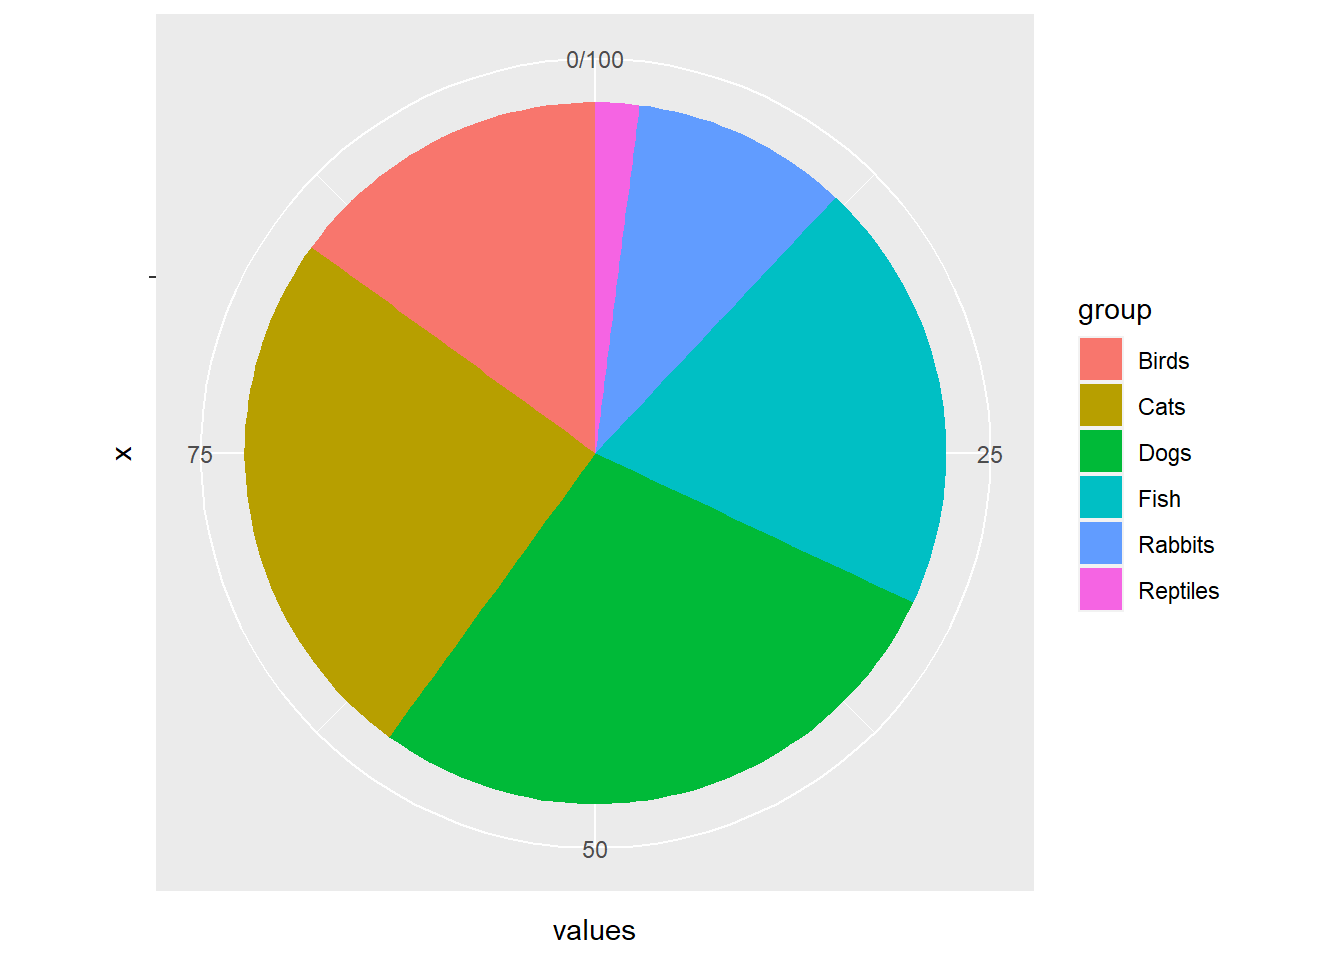
\includegraphics{ratrdsvs_files/figure-latex/unnamed-chunk-86-1.pdf}
\caption{\label{fig:unnamed-chunk-86}A ggplot object with a geom\_point layer, the price of diamonds by their carat, black \& white theme}
\end{figure}

There are lots of different themes in ggplot. If you run that code again you can change \texttt{theme\_bw()} to any of the following:

\begin{itemize}
\item
  \texttt{theme\_classic()}
\item
  \texttt{theme\_grey()}
\item
  \texttt{theme\_light()}
\item
  \texttt{theme\_linedraw()}
\item
  \texttt{theme\_minimal()}
\item
  \texttt{theme\_void()}
\end{itemize}

Which one do you prefer?

Personally, I like this option:

\begin{Shaded}
\begin{Highlighting}[]
\NormalTok{diamonds }\OperatorTok\StringTok{ }
\StringTok{  }\KeywordTok{ggplot}\NormalTok{(}\KeywordTok{aes}\NormalTok{(}\DataTypeTok{x =}\NormalTok{ carat, }\DataTypeTok{y =}\NormalTok{ price)) }\OperatorTok{+}\StringTok{ }
\StringTok{  }\KeywordTok{geom_point}\NormalTok{() }\OperatorTok{+}
\StringTok{  }\KeywordTok{scale_x_continuous}\NormalTok{(}\DataTypeTok{breaks =} \KeywordTok{seq}\NormalTok{ (}\DecValTok{0}\NormalTok{, }\DecValTok{6}\NormalTok{, }\FloatTok{0.5}\NormalTok{), }\DataTypeTok{limits =} \KeywordTok{c}\NormalTok{(}\DecValTok{0}\NormalTok{, }\DecValTok{6}\NormalTok{)) }\OperatorTok{+}\StringTok{ }
\StringTok{  }\KeywordTok{scale_y_continuous}\NormalTok{(}\DataTypeTok{breaks =} \KeywordTok{seq}\NormalTok{(}\DecValTok{0}\NormalTok{, }\DecValTok{20000}\NormalTok{, }\DecValTok{2500}\NormalTok{), }\DataTypeTok{limits =} \KeywordTok{c}\NormalTok{(}\DecValTok{0}\NormalTok{, }\DecValTok{20000}\NormalTok{)) }\OperatorTok{+}
\StringTok{  }\KeywordTok{theme_classic}\NormalTok{() }
\end{Highlighting}
\end{Shaded}

\begin{figure}
\centering
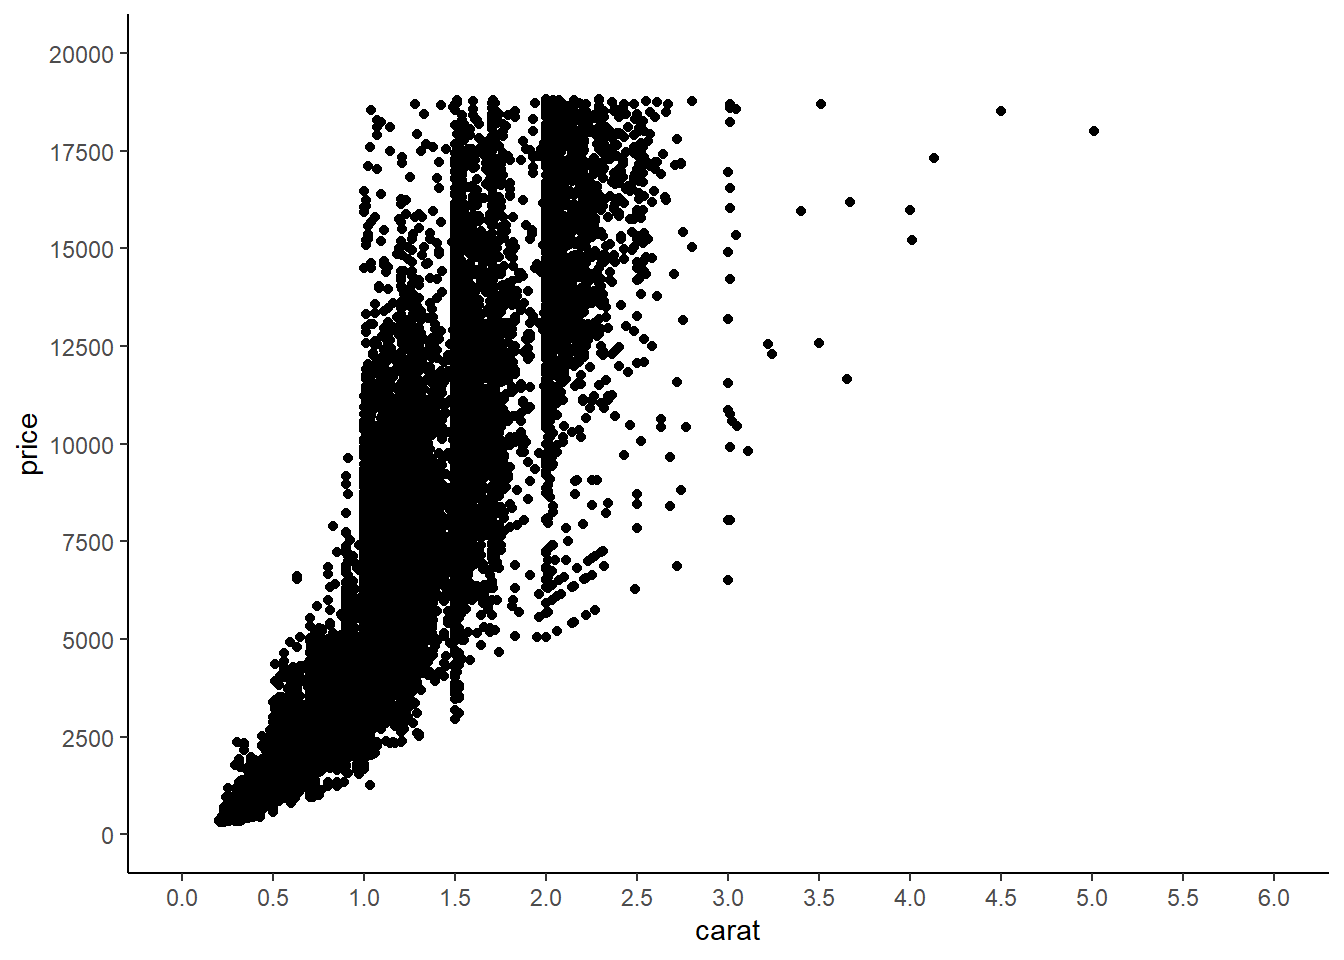
\includegraphics{ratrdsvs_files/figure-latex/unnamed-chunk-87-1.pdf}
\caption{\label{fig:unnamed-chunk-87}A ggplot object with a geom\_point layer, the price of diamonds by their carat, classic theme}
\end{figure}

\hypertarget{gg_labs}{%
\subsection{Changing labels and titles}\label{gg_labs}}

Now we've changed axes, plot area, and gridlines, why don't we give this beautiful plot some labels?

\begin{hey}
If you were to take a wild guess at how to change labels - what would
you add to the plot?

Remember, taking the time to stop and try these exercises will help you
learn R.

And remember that R Studio will autocomplete things you type - what
happens if you start to type `labels'?
\end{hey}

We can adjust labels with the following extra line of code.

\begin{Shaded}
\begin{Highlighting}[]
\NormalTok{diamonds }\OperatorTok\StringTok{ }
\StringTok{  }\KeywordTok{ggplot}\NormalTok{(}\KeywordTok{aes}\NormalTok{(}\DataTypeTok{x =}\NormalTok{ carat, }\DataTypeTok{y =}\NormalTok{ price)) }\OperatorTok{+}\StringTok{ }
\StringTok{  }\KeywordTok{geom_point}\NormalTok{() }\OperatorTok{+}
\StringTok{  }\KeywordTok{scale_x_continuous}\NormalTok{(}\DataTypeTok{breaks =} \KeywordTok{seq}\NormalTok{ (}\DecValTok{0}\NormalTok{, }\DecValTok{6}\NormalTok{, }\FloatTok{0.5}\NormalTok{), }\DataTypeTok{limits =} \KeywordTok{c}\NormalTok{(}\DecValTok{0}\NormalTok{, }\DecValTok{6}\NormalTok{)) }\OperatorTok{+}\StringTok{ }
\StringTok{  }\KeywordTok{scale_y_continuous}\NormalTok{(}\DataTypeTok{breaks =} \KeywordTok{seq}\NormalTok{(}\DecValTok{0}\NormalTok{, }\DecValTok{20000}\NormalTok{, }\DecValTok{2500}\NormalTok{), }\DataTypeTok{limits =} \KeywordTok{c}\NormalTok{(}\DecValTok{0}\NormalTok{, }\DecValTok{20000}\NormalTok{)) }\OperatorTok{+}
\StringTok{  }\KeywordTok{theme_classic}\NormalTok{() }\OperatorTok{+}
\StringTok{  }\KeywordTok{labs}\NormalTok{ (}\DataTypeTok{x =} \StringTok{"Carat (a measure of diamond weight)"}\NormalTok{)}
\end{Highlighting}
\end{Shaded}

\begin{figure}
\centering
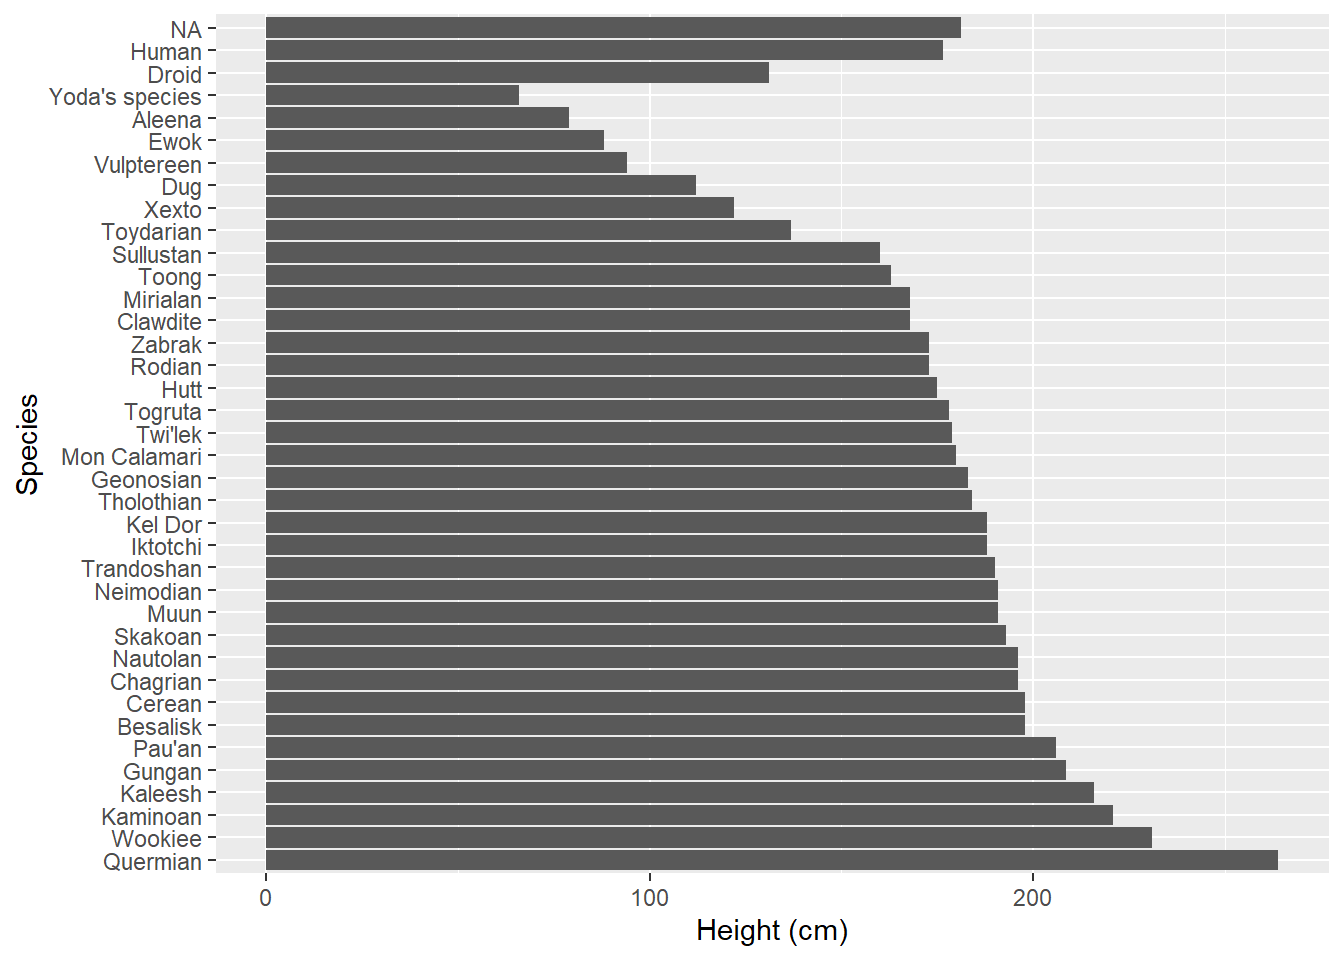
\includegraphics{ratrdsvs_files/figure-latex/unnamed-chunk-89-1.pdf}
\caption{\label{fig:unnamed-chunk-89}A ggplot object with a geom\_point layer, the price of diamonds by their carat, adjusted labels}
\end{figure}

Unsurprisingly, if we want to change the y axis label, we just need to add another argument inside the \texttt{labs()}.

\begin{Shaded}
\begin{Highlighting}[]
\NormalTok{diamonds }\OperatorTok\StringTok{ }
\StringTok{  }\KeywordTok{ggplot}\NormalTok{(}\KeywordTok{aes}\NormalTok{(}\DataTypeTok{x =}\NormalTok{ carat, }\DataTypeTok{y =}\NormalTok{ price)) }\OperatorTok{+}\StringTok{ }
\StringTok{  }\KeywordTok{geom_point}\NormalTok{() }\OperatorTok{+}
\StringTok{  }\KeywordTok{scale_x_continuous}\NormalTok{(}\DataTypeTok{breaks =} \KeywordTok{seq}\NormalTok{ (}\DecValTok{0}\NormalTok{, }\DecValTok{6}\NormalTok{, }\FloatTok{0.5}\NormalTok{), }\DataTypeTok{limits =} \KeywordTok{c}\NormalTok{(}\DecValTok{0}\NormalTok{, }\DecValTok{6}\NormalTok{)) }\OperatorTok{+}\StringTok{ }
\StringTok{  }\KeywordTok{scale_y_continuous}\NormalTok{(}\DataTypeTok{breaks =} \KeywordTok{seq}\NormalTok{(}\DecValTok{0}\NormalTok{, }\DecValTok{20000}\NormalTok{, }\DecValTok{2500}\NormalTok{), }\DataTypeTok{limits =} \KeywordTok{c}\NormalTok{(}\DecValTok{0}\NormalTok{, }\DecValTok{20000}\NormalTok{)) }\OperatorTok{+}
\StringTok{  }\KeywordTok{theme_classic}\NormalTok{() }\OperatorTok{+}
\StringTok{  }\KeywordTok{labs}\NormalTok{ (}\DataTypeTok{x =} \StringTok{"Carat (a measure of diamond weight)"}\NormalTok{,}
        \DataTypeTok{y =} \StringTok{"Price in US dollars ($)"}\NormalTok{)}
\end{Highlighting}
\end{Shaded}

\begin{figure}
\centering
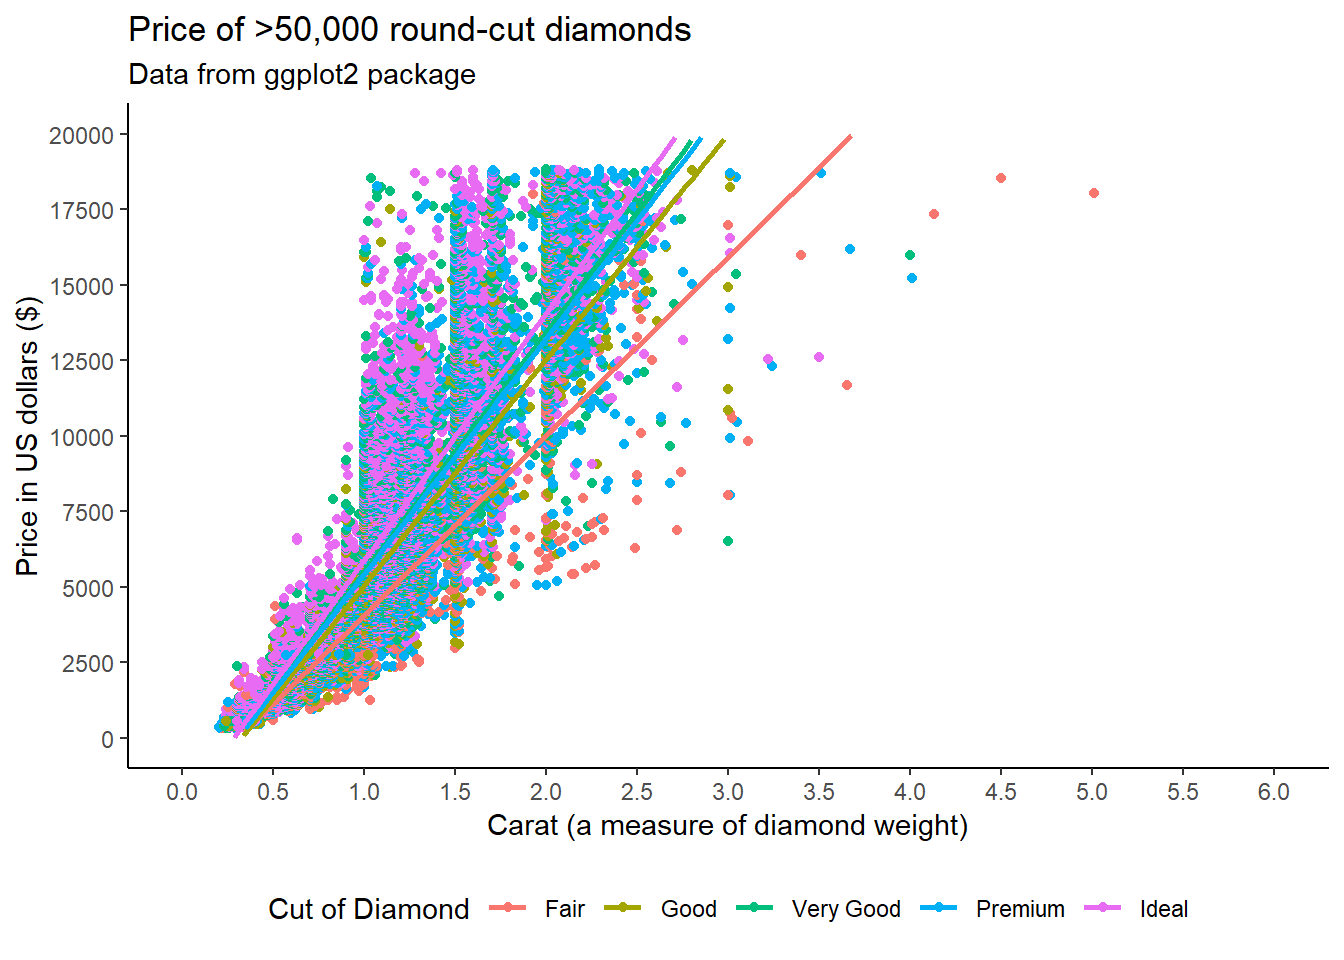
\includegraphics{ratrdsvs_files/figure-latex/unnamed-chunk-90-1.pdf}
\caption{\label{fig:unnamed-chunk-90}A ggplot object with a geom\_point layer, the price of diamonds by their carat, adjusted labels}
\end{figure}

You can even add in titles and subtitles.

\begin{Shaded}
\begin{Highlighting}[]
\NormalTok{diamonds }\OperatorTok\StringTok{ }
\StringTok{  }\KeywordTok{ggplot}\NormalTok{(}\KeywordTok{aes}\NormalTok{(}\DataTypeTok{x =}\NormalTok{ carat, }\DataTypeTok{y =}\NormalTok{ price)) }\OperatorTok{+}\StringTok{ }
\StringTok{  }\KeywordTok{geom_point}\NormalTok{() }\OperatorTok{+}
\StringTok{  }\KeywordTok{scale_x_continuous}\NormalTok{(}\DataTypeTok{breaks =} \KeywordTok{seq}\NormalTok{ (}\DecValTok{0}\NormalTok{, }\DecValTok{6}\NormalTok{, }\FloatTok{0.5}\NormalTok{), }\DataTypeTok{limits =} \KeywordTok{c}\NormalTok{(}\DecValTok{0}\NormalTok{, }\DecValTok{6}\NormalTok{)) }\OperatorTok{+}\StringTok{ }
\StringTok{  }\KeywordTok{scale_y_continuous}\NormalTok{(}\DataTypeTok{breaks =} \KeywordTok{seq}\NormalTok{(}\DecValTok{0}\NormalTok{, }\DecValTok{20000}\NormalTok{, }\DecValTok{2500}\NormalTok{), }\DataTypeTok{limits =} \KeywordTok{c}\NormalTok{(}\DecValTok{0}\NormalTok{, }\DecValTok{20000}\NormalTok{)) }\OperatorTok{+}
\StringTok{  }\KeywordTok{theme_classic}\NormalTok{() }\OperatorTok{+}
\StringTok{  }\KeywordTok{labs}\NormalTok{ (}\DataTypeTok{x =} \StringTok{"Carat (a measure of diamond weight)"}\NormalTok{,}
        \DataTypeTok{y =} \StringTok{"Price in US dollars ($)"}\NormalTok{,}
        \DataTypeTok{title =} \StringTok{"Price of >50,000 round-cut diamonds"}\NormalTok{,}
        \DataTypeTok{subtitle =} \StringTok{"Data from ggplot2 package"}\NormalTok{)}
\end{Highlighting}
\end{Shaded}

\begin{figure}
\centering
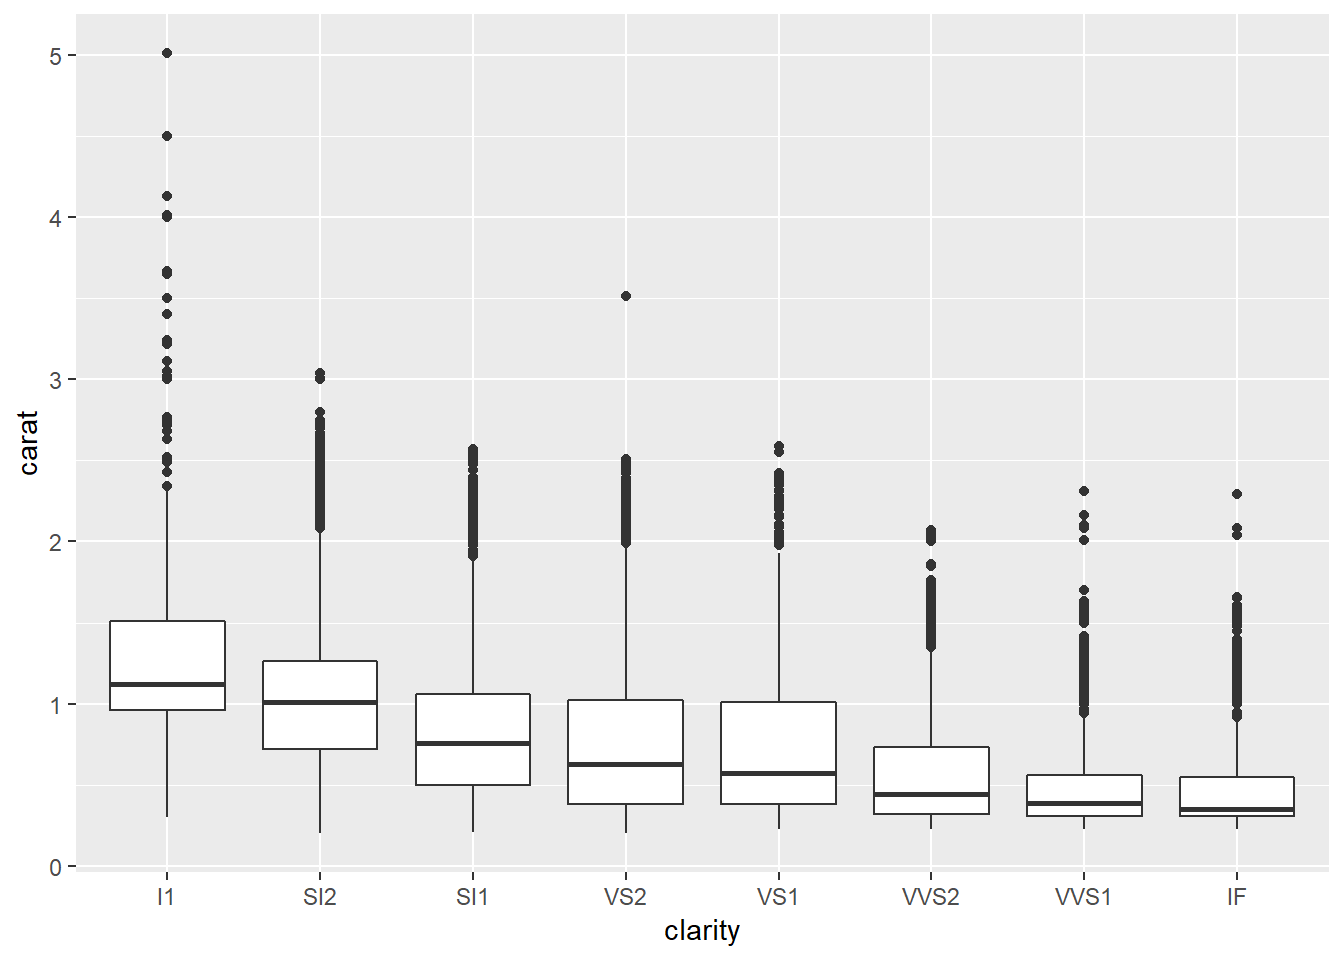
\includegraphics{ratrdsvs_files/figure-latex/unnamed-chunk-91-1.pdf}
\caption{\label{fig:unnamed-chunk-91}A ggplot object with a geom\_point layer, the price of diamonds by their carat, adjusted labels}
\end{figure}

\hypertarget{gg_smooth}{%
\subsection{Adding regression lines to ggplot}\label{gg_smooth}}

It seems as though the bigger the diamond is, the more you pay for it, so why don't we add a line of best fit to demonstrate this?

This is so easy to do in R.

We add:

\begin{translate}
We add to the graph a smooth line geom (\texttt{stat\_smooth})

We have a number of options here:

\begin{itemize}
\item
  We want the line to be calculated using a linear model
  (\texttt{method\ =\ "lm"})
\item
  We don't want to see any standard error bars around the line
  (\texttt{se\ =\ FALSE})
\end{itemize}
\end{translate}

\begin{Shaded}
\begin{Highlighting}[]
\NormalTok{diamonds }\OperatorTok\StringTok{ }
\StringTok{  }\KeywordTok{ggplot}\NormalTok{(}\KeywordTok{aes}\NormalTok{(}\DataTypeTok{x =}\NormalTok{ carat, }\DataTypeTok{y =}\NormalTok{ price)) }\OperatorTok{+}\StringTok{ }
\StringTok{  }\KeywordTok{geom_point}\NormalTok{() }\OperatorTok{+}
\StringTok{  }\KeywordTok{scale_x_continuous}\NormalTok{(}\DataTypeTok{breaks =} \KeywordTok{seq}\NormalTok{ (}\DecValTok{0}\NormalTok{, }\DecValTok{6}\NormalTok{, }\FloatTok{0.5}\NormalTok{), }\DataTypeTok{limits =} \KeywordTok{c}\NormalTok{(}\DecValTok{0}\NormalTok{, }\DecValTok{6}\NormalTok{)) }\OperatorTok{+}\StringTok{ }
\StringTok{  }\KeywordTok{scale_y_continuous}\NormalTok{(}\DataTypeTok{breaks =} \KeywordTok{seq}\NormalTok{(}\DecValTok{0}\NormalTok{, }\DecValTok{20000}\NormalTok{, }\DecValTok{2500}\NormalTok{), }\DataTypeTok{limits =} \KeywordTok{c}\NormalTok{(}\DecValTok{0}\NormalTok{, }\DecValTok{20000}\NormalTok{)) }\OperatorTok{+}
\StringTok{  }\KeywordTok{theme_classic}\NormalTok{() }\OperatorTok{+}
\StringTok{  }\KeywordTok{labs}\NormalTok{ (}\DataTypeTok{x =} \StringTok{"Carat (a measure of diamond weight)"}\NormalTok{,}
        \DataTypeTok{y =} \StringTok{"Price in US dollars ($)"}\NormalTok{,}
        \DataTypeTok{title =} \StringTok{"Price of >50,000 round-cut diamonds"}\NormalTok{,}
        \DataTypeTok{subtitle =} \StringTok{"Data from ggplot2 package"}\NormalTok{) }\OperatorTok{+}\StringTok{ }
\StringTok{  }\KeywordTok{stat_smooth}\NormalTok{(}\DataTypeTok{method =} \StringTok{"lm"}\NormalTok{, }\DataTypeTok{se =} \OtherTok{FALSE}\NormalTok{)}
\end{Highlighting}
\end{Shaded}

\begin{figure}
\centering
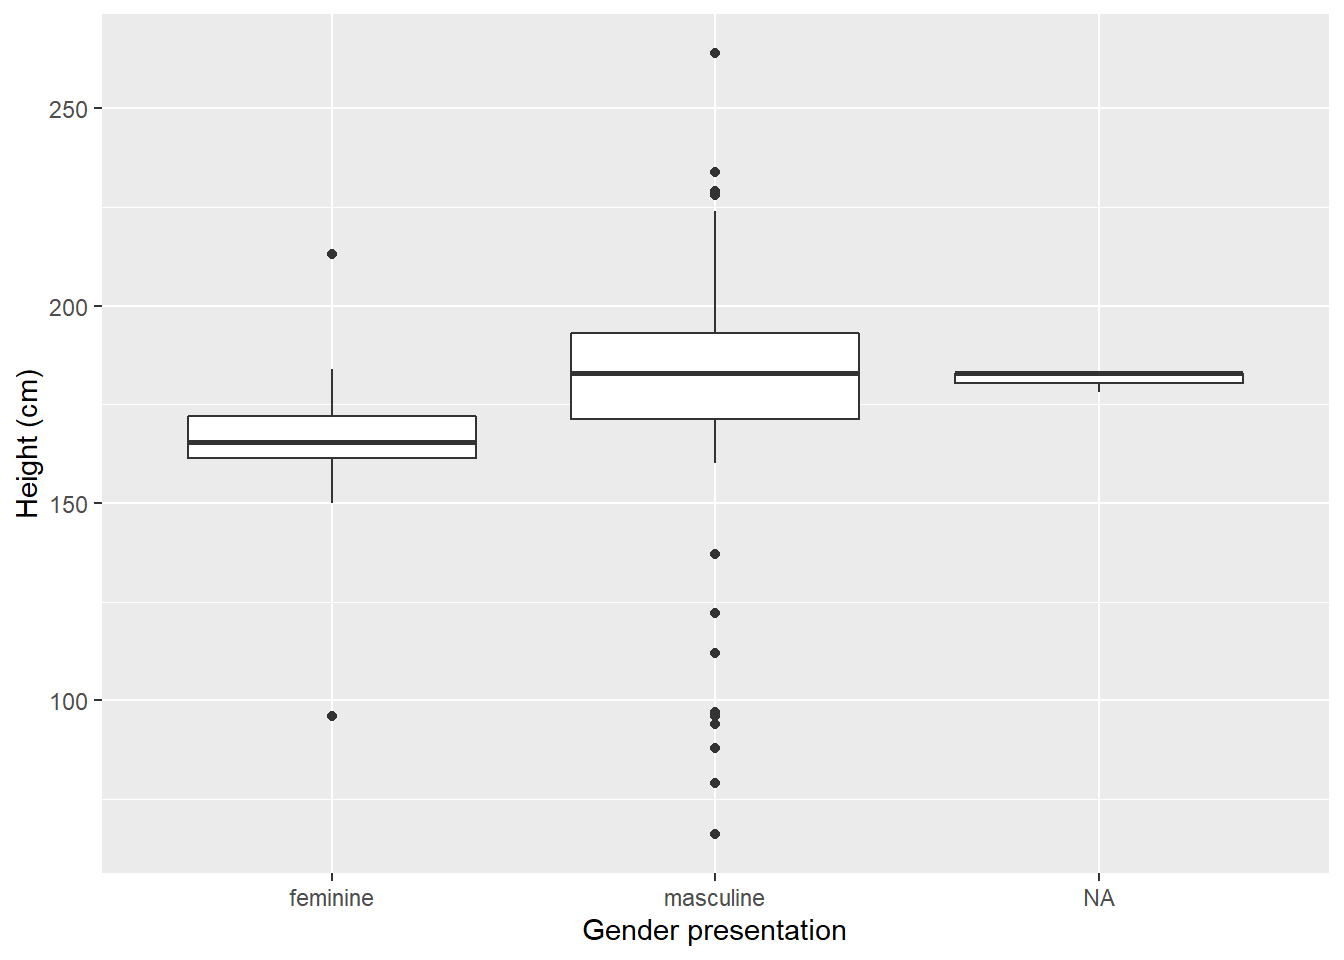
\includegraphics{ratrdsvs_files/figure-latex/unnamed-chunk-93-1.pdf}
\caption{\label{fig:unnamed-chunk-93}A ggplot object with a geom\_point layer, the price of diamonds by their carat, regression line added}
\end{figure}

\hypertarget{gg_groups}{%
\subsection{Adding groups to ggplot}\label{gg_groups}}

Looking at our plot, it seems clear that the diamonds seem to stagger a bit, with lots of diamonds at 1, 1.5, 2, 3, and 3.5 carats, and fewer diamonds in the middle of a carat range. There may be something else in the data that helps to explain this . . .

In ggplot, we can easily add a grouping variable to a scatterplot.

All we need to do, is give it a new aesthetic (\texttt{aes}) argument: \texttt{colour\ =\ cut}.

\begin{Shaded}
\begin{Highlighting}[]
\NormalTok{diamonds }\OperatorTok\StringTok{ }
\StringTok{  }\KeywordTok{ggplot}\NormalTok{(}\KeywordTok{aes}\NormalTok{(}\DataTypeTok{x =}\NormalTok{ carat, }\DataTypeTok{y =}\NormalTok{ price, }\DataTypeTok{colour =}\NormalTok{ cut)) }\OperatorTok{+}\StringTok{ }
\StringTok{  }\KeywordTok{geom_point}\NormalTok{() }\OperatorTok{+}
\StringTok{  }\KeywordTok{scale_x_continuous}\NormalTok{(}\DataTypeTok{breaks =} \KeywordTok{seq}\NormalTok{ (}\DecValTok{0}\NormalTok{, }\DecValTok{6}\NormalTok{, }\FloatTok{0.5}\NormalTok{), }\DataTypeTok{limits =} \KeywordTok{c}\NormalTok{(}\DecValTok{0}\NormalTok{, }\DecValTok{6}\NormalTok{)) }\OperatorTok{+}\StringTok{ }
\StringTok{  }\KeywordTok{scale_y_continuous}\NormalTok{(}\DataTypeTok{breaks =} \KeywordTok{seq}\NormalTok{(}\DecValTok{0}\NormalTok{, }\DecValTok{20000}\NormalTok{, }\DecValTok{2500}\NormalTok{), }\DataTypeTok{limits =} \KeywordTok{c}\NormalTok{(}\DecValTok{0}\NormalTok{, }\DecValTok{20000}\NormalTok{)) }\OperatorTok{+}
\StringTok{  }\KeywordTok{theme_classic}\NormalTok{() }\OperatorTok{+}
\StringTok{  }\KeywordTok{labs}\NormalTok{ (}\DataTypeTok{x =} \StringTok{"Carat (a measure of diamond weight)"}\NormalTok{,}
        \DataTypeTok{y =} \StringTok{"Price in US dollars ($)"}\NormalTok{,}
        \DataTypeTok{title =} \StringTok{"Price of >50,000 round-cut diamonds"}\NormalTok{,}
        \DataTypeTok{subtitle =} \StringTok{"Data from ggplot2 package"}\NormalTok{) }\OperatorTok{+}\StringTok{ }
\StringTok{  }\KeywordTok{stat_smooth}\NormalTok{(}\DataTypeTok{method =} \StringTok{"lm"}\NormalTok{, }\DataTypeTok{se =} \OtherTok{FALSE}\NormalTok{)}
\end{Highlighting}
\end{Shaded}

\begin{figure}
\centering
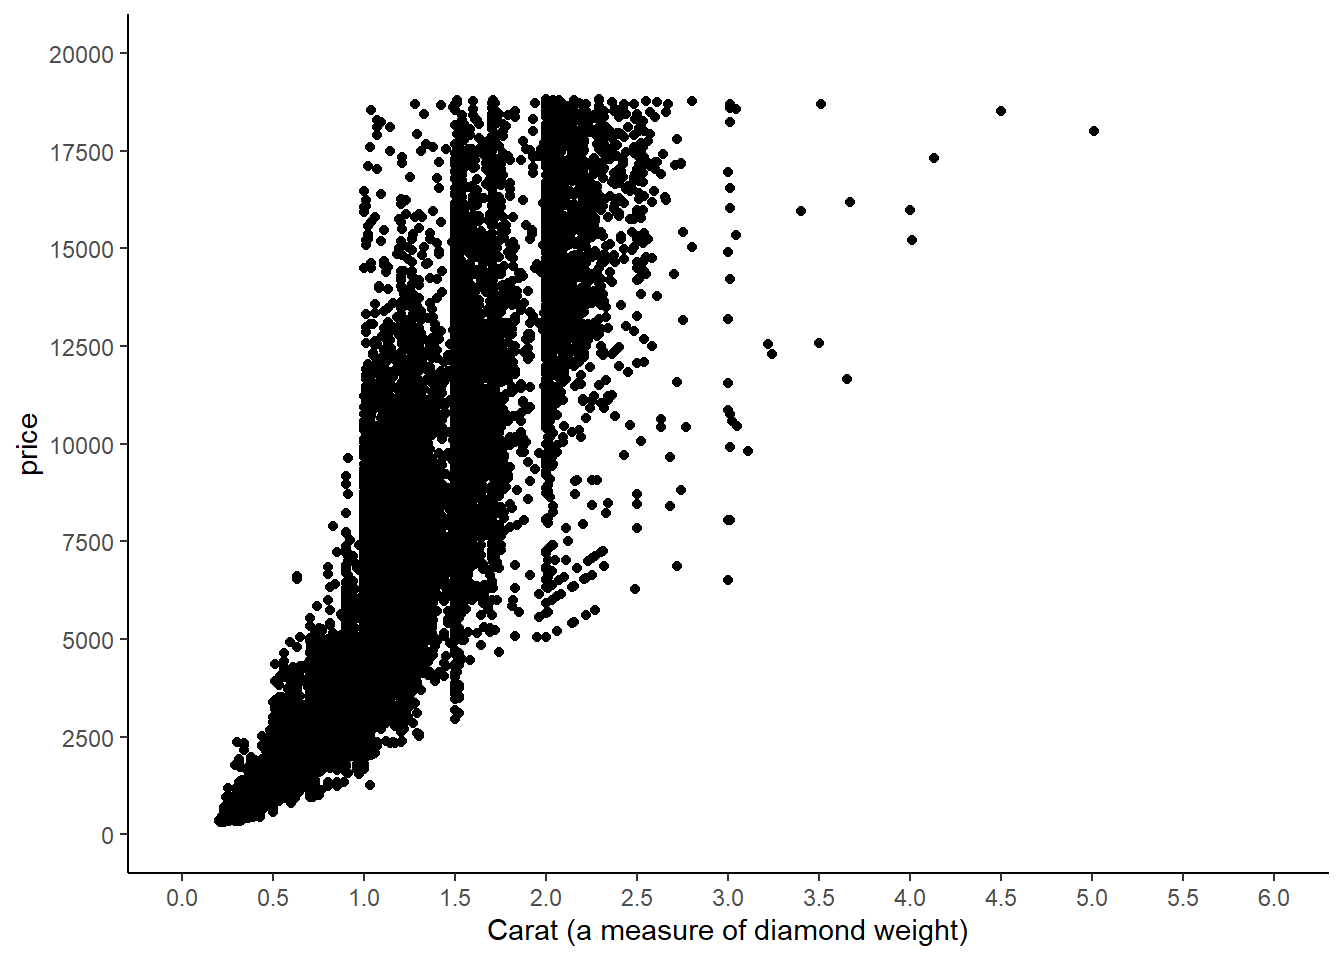
\includegraphics{ratrdsvs_files/figure-latex/unnamed-chunk-94-1.pdf}
\caption{\label{fig:unnamed-chunk-94}A ggplot object with a geom\_point layer, the price of diamonds by their carat and cut, regression line added}
\end{figure}

This has done quite a lot to our chart - its given us several new lines for each group, and a legend. If your computer is anything like mine, it might be starting to take a few seconds to render this chart. Let's just do one more thing before we stop playing with this chart.

\hypertarget{gg_legend}{%
\subsection{Changing legends}\label{gg_legend}}

Using the \texttt{theme()} argument (which is subtly different from the \texttt{theme\_classic()} command), we can adjust the legend.

\begin{Shaded}
\begin{Highlighting}[]
\NormalTok{diamonds }\OperatorTok\StringTok{ }
\StringTok{  }\KeywordTok{ggplot}\NormalTok{(}\KeywordTok{aes}\NormalTok{(}\DataTypeTok{x =}\NormalTok{ carat, }\DataTypeTok{y =}\NormalTok{ price, }\DataTypeTok{colour =}\NormalTok{ cut)) }\OperatorTok{+}\StringTok{ }
\StringTok{  }\KeywordTok{geom_point}\NormalTok{() }\OperatorTok{+}
\StringTok{  }\KeywordTok{scale_x_continuous}\NormalTok{(}\DataTypeTok{breaks =} \KeywordTok{seq}\NormalTok{ (}\DecValTok{0}\NormalTok{, }\DecValTok{6}\NormalTok{, }\FloatTok{0.5}\NormalTok{), }\DataTypeTok{limits =} \KeywordTok{c}\NormalTok{(}\DecValTok{0}\NormalTok{, }\DecValTok{6}\NormalTok{)) }\OperatorTok{+}\StringTok{ }
\StringTok{  }\KeywordTok{scale_y_continuous}\NormalTok{(}\DataTypeTok{breaks =} \KeywordTok{seq}\NormalTok{(}\DecValTok{0}\NormalTok{, }\DecValTok{20000}\NormalTok{, }\DecValTok{2500}\NormalTok{), }\DataTypeTok{limits =} \KeywordTok{c}\NormalTok{(}\DecValTok{0}\NormalTok{, }\DecValTok{20000}\NormalTok{)) }\OperatorTok{+}
\StringTok{  }\KeywordTok{theme_classic}\NormalTok{() }\OperatorTok{+}
\StringTok{  }\KeywordTok{labs}\NormalTok{ (}\DataTypeTok{x =} \StringTok{"Carat (a measure of diamond weight)"}\NormalTok{,}
        \DataTypeTok{y =} \StringTok{"Price in US dollars ($)"}\NormalTok{,}
        \DataTypeTok{title =} \StringTok{"Price of >50,000 round-cut diamonds"}\NormalTok{,}
        \DataTypeTok{subtitle =} \StringTok{"Data from ggplot2 package"}\NormalTok{) }\OperatorTok{+}\StringTok{ }
\StringTok{  }\KeywordTok{stat_smooth}\NormalTok{(}\DataTypeTok{method =} \StringTok{"lm"}\NormalTok{, }\DataTypeTok{se =} \OtherTok{FALSE}\NormalTok{) }\OperatorTok{+}
\StringTok{  }\KeywordTok{theme}\NormalTok{(}\DataTypeTok{legend.position =} \StringTok{"bottom"}\NormalTok{)}
\end{Highlighting}
\end{Shaded}

\begin{figure}
\centering
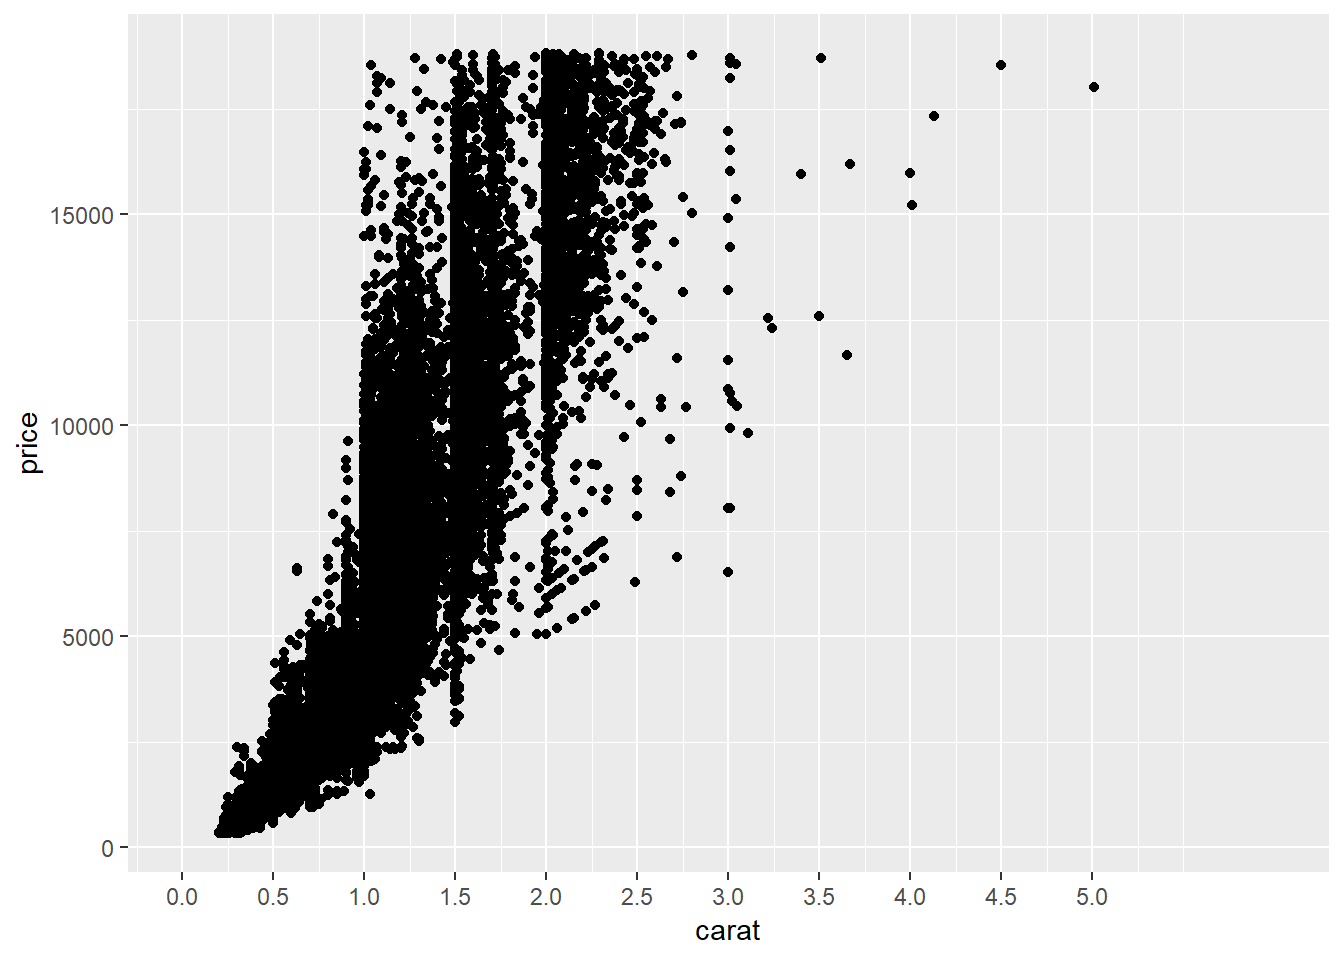
\includegraphics{ratrdsvs_files/figure-latex/unnamed-chunk-95-1.pdf}
\caption{\label{fig:unnamed-chunk-95}A ggplot object with a geom\_point layer, the price of diamonds by their carat and cut, regression line added}
\end{figure}

But lets say we also want to change the text from `cut' to `Cut of Diamond'. Well, you can think of this as another axis we can change. Instead of a \texttt{scale\_x\_} we can change the \texttt{scale\_colour\_}. And this isn't a continuous scale but a discrete (categorical) one, so we change it with \texttt{scale\_colour\_discrete}.

\begin{Shaded}
\begin{Highlighting}[]
\NormalTok{diamonds }\OperatorTok\StringTok{ }
\StringTok{  }\KeywordTok{ggplot}\NormalTok{(}\KeywordTok{aes}\NormalTok{(}\DataTypeTok{x =}\NormalTok{ carat, }\DataTypeTok{y =}\NormalTok{ price, }\DataTypeTok{colour =}\NormalTok{ cut)) }\OperatorTok{+}\StringTok{ }
\StringTok{  }\KeywordTok{geom_point}\NormalTok{() }\OperatorTok{+}
\StringTok{  }\KeywordTok{scale_x_continuous}\NormalTok{(}\DataTypeTok{breaks =} \KeywordTok{seq}\NormalTok{ (}\DecValTok{0}\NormalTok{, }\DecValTok{6}\NormalTok{, }\FloatTok{0.5}\NormalTok{), }\DataTypeTok{limits =} \KeywordTok{c}\NormalTok{(}\DecValTok{0}\NormalTok{, }\DecValTok{6}\NormalTok{)) }\OperatorTok{+}\StringTok{ }
\StringTok{  }\KeywordTok{scale_y_continuous}\NormalTok{(}\DataTypeTok{breaks =} \KeywordTok{seq}\NormalTok{(}\DecValTok{0}\NormalTok{, }\DecValTok{20000}\NormalTok{, }\DecValTok{2500}\NormalTok{), }\DataTypeTok{limits =} \KeywordTok{c}\NormalTok{(}\DecValTok{0}\NormalTok{, }\DecValTok{20000}\NormalTok{)) }\OperatorTok{+}
\StringTok{  }\KeywordTok{theme_classic}\NormalTok{() }\OperatorTok{+}
\StringTok{  }\KeywordTok{labs}\NormalTok{ (}\DataTypeTok{x =} \StringTok{"Carat (a measure of diamond weight)"}\NormalTok{,}
        \DataTypeTok{y =} \StringTok{"Price in US dollars ($)"}\NormalTok{,}
        \DataTypeTok{title =} \StringTok{"Price of >50,000 round-cut diamonds"}\NormalTok{,}
        \DataTypeTok{subtitle =} \StringTok{"Data from ggplot2 package"}\NormalTok{) }\OperatorTok{+}\StringTok{ }
\StringTok{  }\KeywordTok{stat_smooth}\NormalTok{(}\DataTypeTok{method =} \StringTok{"lm"}\NormalTok{, }\DataTypeTok{se =} \OtherTok{FALSE}\NormalTok{) }\OperatorTok{+}
\StringTok{  }\KeywordTok{theme}\NormalTok{(}\DataTypeTok{legend.position =} \StringTok{"bottom"}\NormalTok{) }\OperatorTok{+}
\StringTok{  }\KeywordTok{scale_color_discrete}\NormalTok{(}\DataTypeTok{name =} \StringTok{"Cut of Diamond"}\NormalTok{)}
\end{Highlighting}
\end{Shaded}

\begin{figure}
\centering
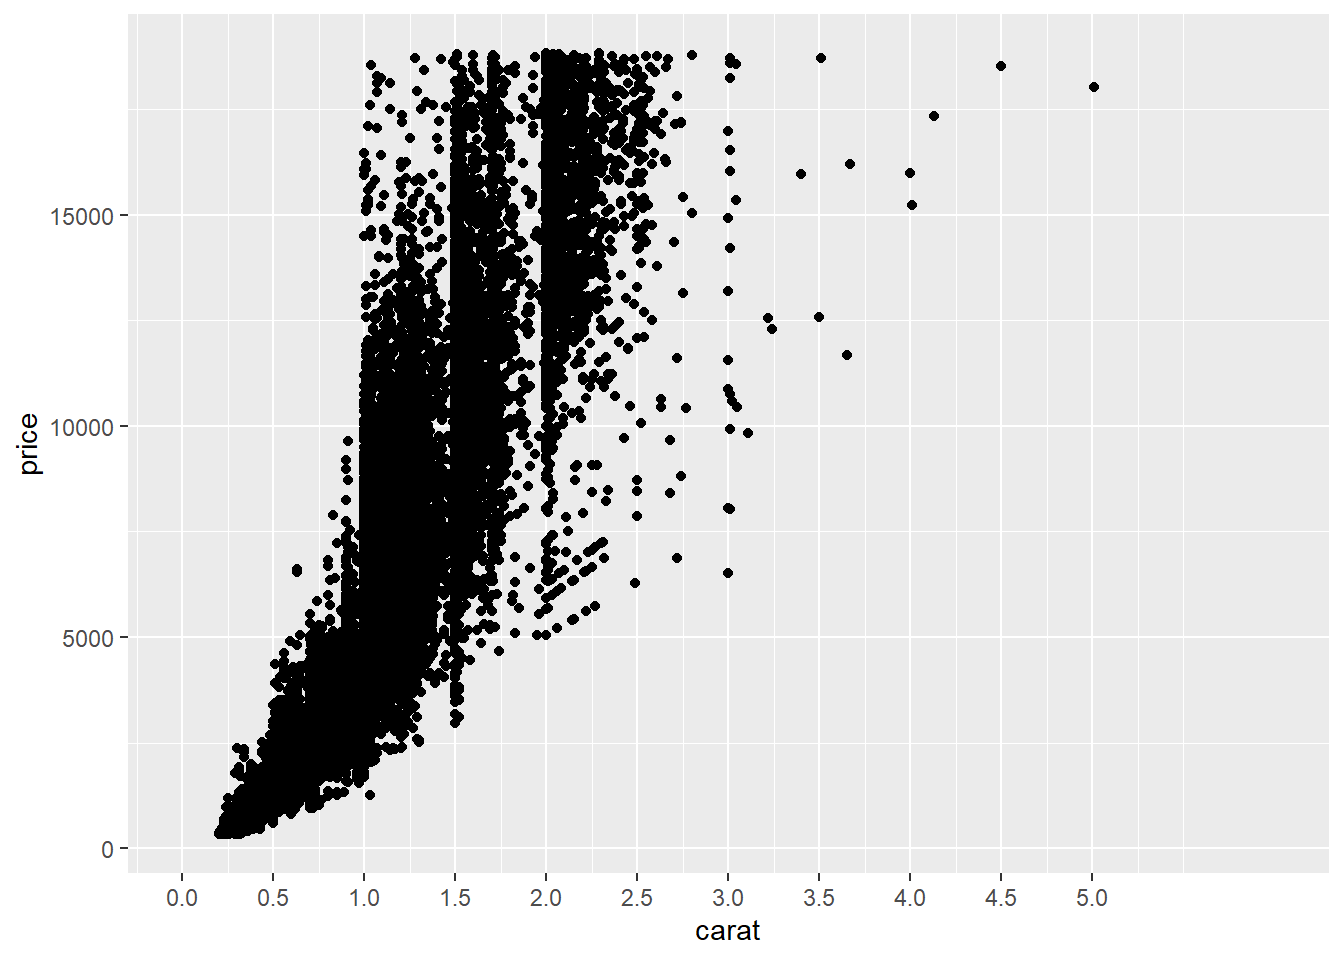
\includegraphics{ratrdsvs_files/figure-latex/unnamed-chunk-96-1.pdf}
\caption{\label{fig:unnamed-chunk-96}A ggplot object with a geom\_point layer, the price of diamonds by their carat and cut, regression line added}
\end{figure}

\hypertarget{gg_boxplot}{%
\section{Building a boxplot}\label{gg_boxplot}}

At this stage, I'm wondering how useful our scatterplot is. Perhaps it would be easier to visualise this with a boxplot. We just need to build a new object.

Lets look to see if there's a relationship between how big the diamond is (carat) and its clarity (how clear it is).

\begin{Shaded}
\begin{Highlighting}[]
\NormalTok{diamonds }\OperatorTok\StringTok{ }
\StringTok{  }\KeywordTok{ggplot}\NormalTok{(}\KeywordTok{aes}\NormalTok{(}\DataTypeTok{x =}\NormalTok{ clarity, }\DataTypeTok{y =}\NormalTok{ carat)) }\OperatorTok{+}\StringTok{ }
\StringTok{  }\KeywordTok{geom_boxplot}\NormalTok{()}
\end{Highlighting}
\end{Shaded}

\begin{figure}
\centering
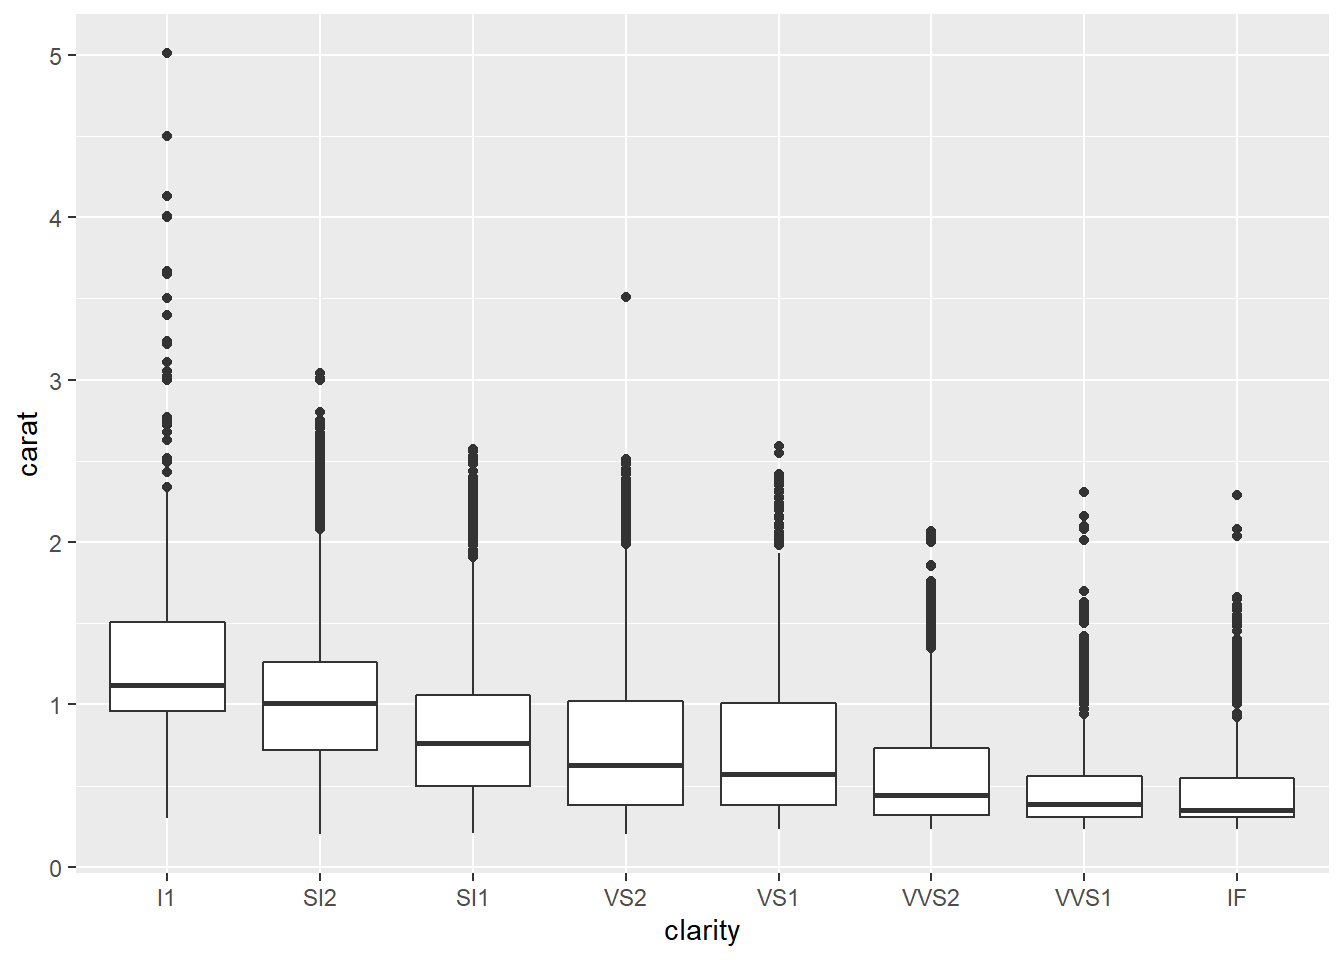
\includegraphics{ratrdsvs_files/figure-latex/unnamed-chunk-97-1.pdf}
\caption{\label{fig:unnamed-chunk-97}A ggplot object with a geom\_boxplot, the carat of diamonds by their clarity}
\end{figure}

And with just a few lines of code, we can create a very different looking chart:

\begin{Shaded}
\begin{Highlighting}[]
\NormalTok{diamonds }\OperatorTok\StringTok{ }
\StringTok{  }\KeywordTok{ggplot}\NormalTok{(}\KeywordTok{aes}\NormalTok{(}\DataTypeTok{x =}\NormalTok{ clarity, }\DataTypeTok{y =}\NormalTok{ carat, }\DataTypeTok{colour =}\NormalTok{ clarity)) }\OperatorTok{+}\StringTok{ }
\StringTok{  }\KeywordTok{geom_boxplot}\NormalTok{() }\OperatorTok{+}
\StringTok{  }\KeywordTok{labs}\NormalTok{(}\DataTypeTok{title =} \StringTok{"Clarity and carat of >50,000 diamonds"}\NormalTok{,}
       \DataTypeTok{subtitle =} \StringTok{"Data from ggplot2"}\NormalTok{,}
       \DataTypeTok{x =} \StringTok{"Clarity (clearness) of diamond"}\NormalTok{,}
       \DataTypeTok{y =} \StringTok{"Carat (weight) of diamond"}\NormalTok{) }\OperatorTok{+}\StringTok{ }
\StringTok{  }\KeywordTok{theme_classic}\NormalTok{() }\OperatorTok{+}
\StringTok{  }\KeywordTok{theme}\NormalTok{(}\DataTypeTok{legend.position =} \StringTok{"none"}\NormalTok{)}
\end{Highlighting}
\end{Shaded}

\begin{figure}
\centering
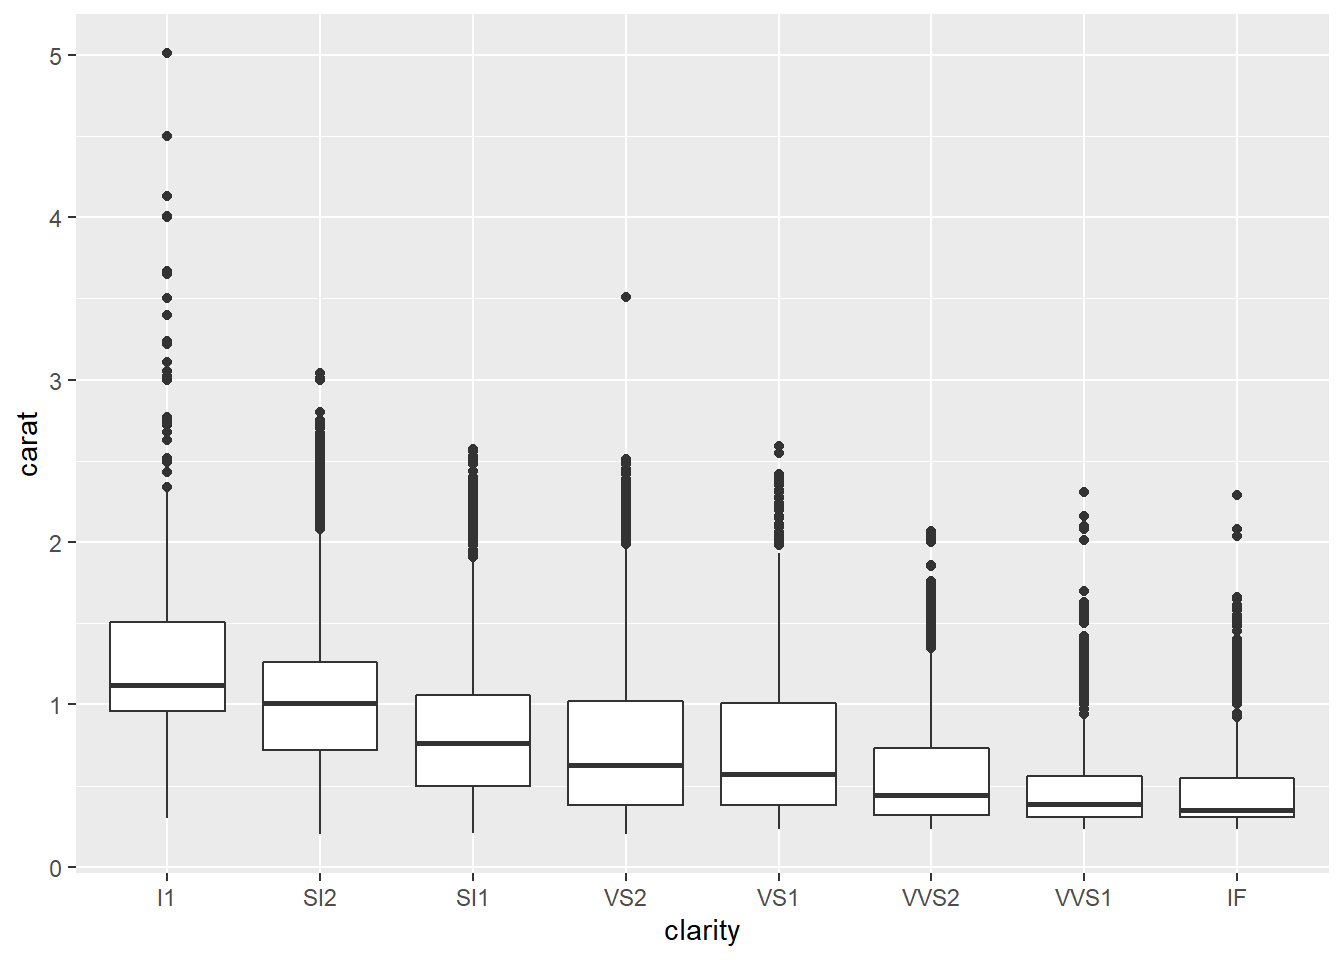
\includegraphics{ratrdsvs_files/figure-latex/unnamed-chunk-98-1.pdf}
\caption{\label{fig:unnamed-chunk-98}A ggplot object with a geom\_boxplot, the carat of diamonds by their clarity}
\end{figure}

\hypertarget{gg_facets}{%
\section{Facets}\label{gg_facets}}

Another very useful command is `facet', which splits one chart into many based on a particular variable.

\begin{Shaded}
\begin{Highlighting}[]
\NormalTok{diamonds }\OperatorTok\StringTok{ }
\StringTok{  }\KeywordTok{ggplot}\NormalTok{(}\KeywordTok{aes}\NormalTok{(}\DataTypeTok{x =}\NormalTok{ clarity, }\DataTypeTok{y =}\NormalTok{ carat, }\DataTypeTok{colour =}\NormalTok{ clarity)) }\OperatorTok{+}\StringTok{ }
\StringTok{  }\KeywordTok{geom_boxplot}\NormalTok{() }\OperatorTok{+}
\StringTok{  }\KeywordTok{labs}\NormalTok{(}\DataTypeTok{title =} \StringTok{"Claritym cut and carat of >50,000 diamonds"}\NormalTok{,}
       \DataTypeTok{subtitle =} \StringTok{"Data from ggplot2"}\NormalTok{,}
       \DataTypeTok{x =} \StringTok{"Clarity (clearness) of diamond"}\NormalTok{,}
       \DataTypeTok{y =} \StringTok{"Carat (weight) of diamond"}\NormalTok{) }\OperatorTok{+}\StringTok{ }
\StringTok{  }\KeywordTok{theme_classic}\NormalTok{() }\OperatorTok{+}
\StringTok{  }\KeywordTok{theme}\NormalTok{(}\DataTypeTok{legend.position =} \StringTok{"none"}\NormalTok{) }\OperatorTok{+}
\StringTok{  }\KeywordTok{facet_wrap}\NormalTok{(}\DataTypeTok{facets =} \OperatorTok{~}\NormalTok{cut)}
\end{Highlighting}
\end{Shaded}

\begin{figure}
\centering
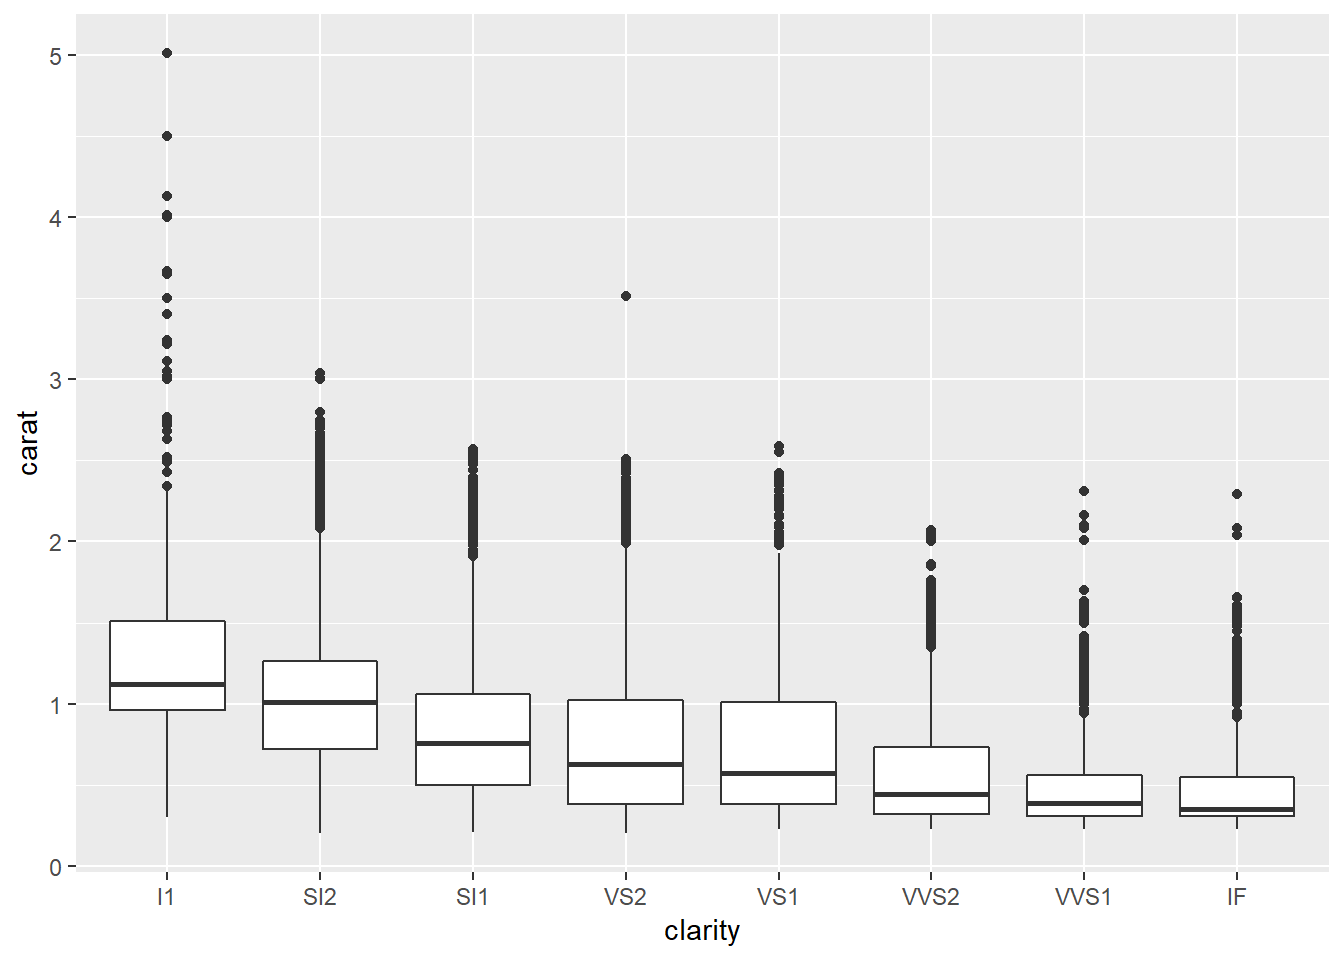
\includegraphics{ratrdsvs_files/figure-latex/unnamed-chunk-99-1.pdf}
\caption{\label{fig:unnamed-chunk-99}A ggplot object with a geom\_boxplot, the carat of diamonds by their clarity}
\end{figure}

\hypertarget{gg_bars}{%
\section{Bar charts}\label{gg_bars}}

To create a bar chart, we simply need to change the \texttt{geom\_boxplot()} to a \texttt{geom\_bar} argument with a \texttt{stat="summary"} specification.

\begin{Shaded}
\begin{Highlighting}[]
\NormalTok{diamonds }\OperatorTok\StringTok{ }
\StringTok{  }\KeywordTok{ggplot}\NormalTok{(}\KeywordTok{aes}\NormalTok{(}\DataTypeTok{x =}\NormalTok{ clarity, }\DataTypeTok{y =}\NormalTok{ carat, }\DataTypeTok{fill =}\NormalTok{ clarity)) }\OperatorTok{+}\StringTok{ }
\StringTok{  }\KeywordTok{geom_bar}\NormalTok{(}\DataTypeTok{stat =} \StringTok{"summary"}\NormalTok{) }\OperatorTok{+}
\StringTok{  }\KeywordTok{labs}\NormalTok{(}\DataTypeTok{title =} \StringTok{"Claritym cut and carat of >50,000 diamonds"}\NormalTok{,}
       \DataTypeTok{subtitle =} \StringTok{"Data from ggplot2"}\NormalTok{,}
       \DataTypeTok{x =} \StringTok{"Clarity (clearness) of diamond"}\NormalTok{,}
       \DataTypeTok{y =} \StringTok{"Carat (weight) of diamond"}\NormalTok{) }\OperatorTok{+}\StringTok{ }
\StringTok{  }\KeywordTok{theme_classic}\NormalTok{() }\OperatorTok{+}
\StringTok{  }\KeywordTok{theme}\NormalTok{(}\DataTypeTok{legend.position =} \StringTok{"none"}\NormalTok{) }\OperatorTok{+}
\StringTok{  }\KeywordTok{facet_wrap}\NormalTok{(}\DataTypeTok{facets =} \OperatorTok{~}\NormalTok{cut)}
\end{Highlighting}
\end{Shaded}

\begin{figure}
\centering
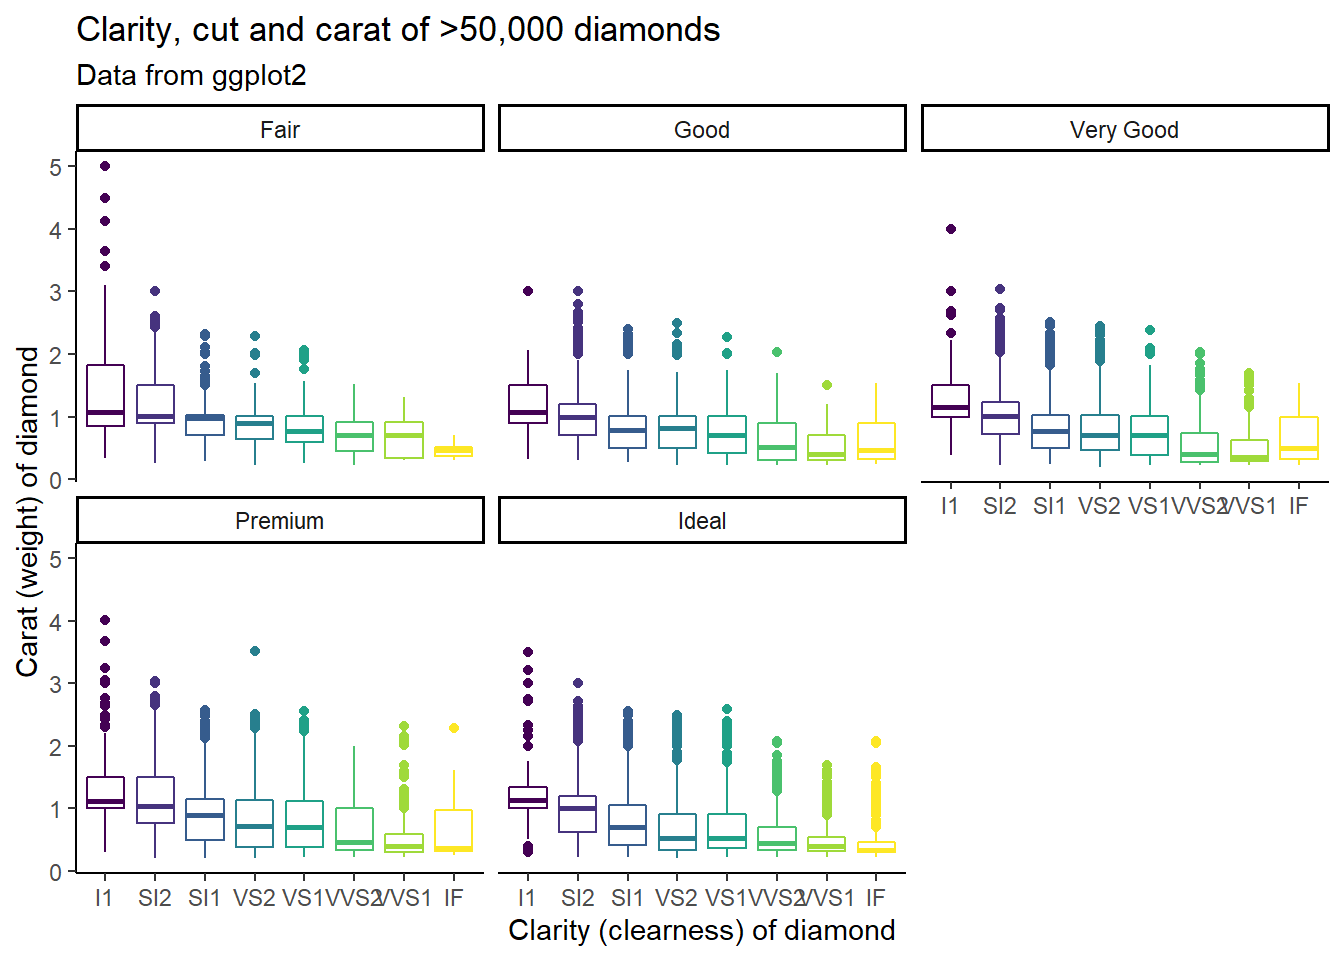
\includegraphics{ratrdsvs_files/figure-latex/unnamed-chunk-100-1.pdf}
\caption{\label{fig:unnamed-chunk-100}A ggplot object with a geom\_bar, the carat of diamonds by their clarity}
\end{figure}

There are a few notes here.

\begin{itemize}
\item
  Within \texttt{geom\_bar} we have set the argument \texttt{geom\_bar(stat\ =\ "summary")}. This tells R to calculate the mean carat for each group (Clarity within cut)
\item
  \texttt{geom\_bar} wants \texttt{fill\ =\ clarity} instead of \texttt{colour\ =\ clarity}, as it treats \texttt{colour} as the line around the bar.
\end{itemize}

\hypertarget{ex_ggplot}{%
\section{Exercise}\label{ex_ggplot}}

Please feel free to google and explore these questions - as well as putting your own customisation touches.

Create a boxplot of the \texttt{mpg} cars dataset, plotting highway miles (\texttt{hwy}) against the car type (\texttt{class})
\protect\hyperlink{gg_answers}{Answer here}

Create a histogram of the number of miles per gallon in the city (\texttt{cty}) faceted by type of transmission (\texttt{trans})
\protect\hyperlink{gg_answers}{Answer here}

\hypertarget{gg_vids}{%
\section{Videos}\label{gg_vids}}

If you'd rather watch a video about this - \href{https://media.ed.ac.uk/media/R+ConversationsA+Demystifying+ggplot/0_sct50ue1}{you can here!}

\hypertarget{gg_resources}{%
\section{Useful resources}\label{gg_resources}}

There are some very useful resources out there about ggplot2 including:

\begin{itemize}
\item
  \href{http://www.cookbook-r.com/Graphs/}{Cookbook for R}, Winston Chang's (free) online book about using ggplot
\item
  \href{https://rstudio.com/wp-content/uploads/2015/03/ggplot2-cheatsheet.pdf}{ggplot cheatsheet}, a pdf with lots of neat visualisations and cheats.
\end{itemize}

\hypertarget{dataprocessing}{%
\chapter{Data Processing}\label{dataprocessing}}

\begin{los}
You can skip this chapter if you:

\begin{itemize}
\item
  Can download, open, edit and save an R Markdown file
\item
  Can describe the advantages of repeatable workflows
\item
  Can execute code in an R Markdown file
\end{itemize}
\end{los}

\hypertarget{workflows}{%
\section{Workflows}\label{workflows}}

Throughout this book, I have been talking about the importance of repeatable workflows.

If you're on a course that I'm teaching, I will share R Markdown documents with you that you can edit and I can view. We could both start with the same dataset, and by sharing our workflow, we can both know exactly what the other person has done. This data transparency is very important. Knowing what changes have been made to the data, and how those changes were made, can help prevent small mistakes being magnified. For example, a simple copy/paste error in excel, resulted in \href{https://www.bbc.co.uk/news/uk-scotland-edinburgh-east-fife-53893101}{an Edinburgh hospital being delivered over two years late}.

You might think this can't apply to you, but think how many times you might make a change to a dataset in the process of cleaning that data and tidying it. If you had to describe what you did to a collaborator, would you remember every change?

One of the great advantages of using code to process data is that every stage can be documented. In this textbook I'm teaching you R, and on my courses I mainly use R Markdown files to document workflows, but R is just one statistical language and R Markdowns are just one file type.

\hypertarget{an-example-of-sharing-code}{%
\subsection{An example of sharing code}\label{an-example-of-sharing-code}}

Imagine you have a big dataset like the UK Farm Accounts dataset:

\begin{verbatim}
##   Year Gross.output.at.basic.prices...million Intermediate.consumption...million Total.Income.from.Farming...million
## 1 1995                               14741.13                           7491.238                           3668.6456
## 2 1996                               14953.92                           7899.517                           3435.5194
## 3 1997                               13334.00                           7471.959                           2028.4870
## 4 1998                               12329.07                           7008.115                           1472.7142
## 5 1999                               11925.87                           6876.278                           1535.0130
## 6 2000                               10962.54                           6483.353                            941.3956
##   Agriculture.s.share.of.total.regional.employment.. Country
## 1                                                 NA England
## 2                                                 NA England
## 3                                                 NA England
## 4                                                 NA England
## 5                                                 NA England
## 6                                           1.319703 England
\end{verbatim}

And let's say you want to explore the gross output of farming per year. You might decided it would be easier to change the name of the gross output variable to make coding easier. So you write the following in the console:

\begin{Shaded}
\begin{Highlighting}[]
\NormalTok{farm <-}\StringTok{ }\NormalTok{farm }\OperatorTok\StringTok{ }
\StringTok{  }\KeywordTok{rename}\NormalTok{(}\DataTypeTok{gross_output =}\NormalTok{ Gross.output.at.basic.prices...million)}
\end{Highlighting}
\end{Shaded}

And then you summarise gross output by year:

\begin{Shaded}
\begin{Highlighting}[]
\NormalTok{farm }\OperatorTok\StringTok{ }
\StringTok{  }\KeywordTok{group_by}\NormalTok{(Year) }\OperatorTok\StringTok{ }
\StringTok{  }\KeywordTok{summarise}\NormalTok{(}\DataTypeTok{mean_gross_output =} \KeywordTok{mean}\NormalTok{(gross_output))}
\end{Highlighting}
\end{Shaded}

\begin{verbatim}
## # A tibble: 25 x 2
##     Year mean_gross_output
##    <int>             <dbl>
##  1  1995             4944.
##  2  1996             5010.
##  3  1997             4474.
##  4  1998             4115.
##  5  1999             3988.
##  6  2000             3744.
##  7  2001             3818.
##  8  2002             3876.
##  9  2003             4033.
## 10  2004             4198.
## # ... with 15 more rows
\end{verbatim}

If you sent the above code chunk to me along with the original dataset, I would not be able to run it. I wouldn't know what variable you had renamed. So at the start of the R Markdown document you would would want to load in the data and run any transformations/changes. That way if you sent me the RMD and the data file, I would be able to replicate what you did exactly.

As a general practice, I aim to follow this structure in my RMD or R script files:

\begin{enumerate}
\def\labelenumi{\arabic{enumi}.}
\tightlist
\item
  Load any libraries that are needed
\item
  Load the data
\item
  Perform any data transformations
\item
  Perform any analyses.
\end{enumerate}

There may be times when there's a good reason to do things in a different order, but you will rarely go wrong with this order (Figure 6.1)

\begin{figure}

{\centering 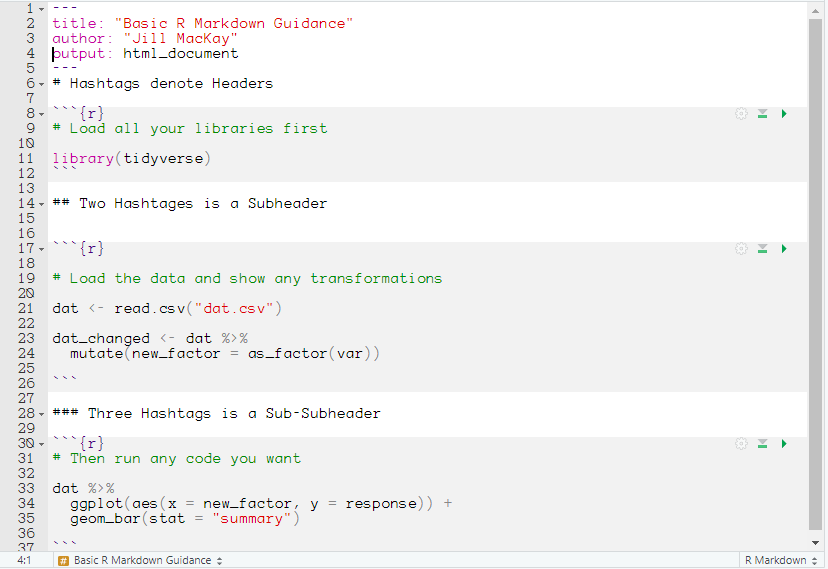
\includegraphics[width=11.5in]{images/06_workflows/example_workflow} 

}

\caption{A general format of R Markdown files}\label{fig:unnamed-chunk-105}
\end{figure}

Sometimes in this book I have suggested using an R Script file instead of an R Markdown file. R Script files are good for short pieces of code, but if you want to talk about your code (say because you're trying to ask your lecturer a question) you might find the ability to type in full paragraphs useful, and that's where R Studio comes in. Some scientists will even write full papers in R Markdown, especially if there's a lot of analyses in them. You can find out more about \href{https://rstudio.com/wp-content/uploads/2015/02/rmarkdown-cheatsheet.pdf}{R Markdown formatting here}.

\hypertarget{openrmd}{%
\section{Opening R Markdown Docs}\label{openrmd}}

R Markdown files work just like any other file in R Studio. You can open any R Markdown file by going to \texttt{File\ \textgreater{}\ Open\ File\ ...} and navigating to the folder your file is stored in.

Your R Markdown file will `look' for any linked files in the same folder its saved in, so if your data is saved in the same folder your R Markdown file is saved in, you can be quite lazy about your directories, e.g.~\texttt{read.csv("data.csv")}. This can be very helpful in repeatable analyses.

\begin{figure}

{\centering \includegraphics{images/06_workflows/openrmd} 

}

\caption{Opening an R Markdown file in R Studio}\label{fig:unnamed-chunk-106}
\end{figure}

\hypertarget{codermd}{%
\section{Running Code}\label{codermd}}

You can run code in R Markdown files by pressing the green `triangle' button to run that specific piece of code.

\begin{figure}

{\centering \includegraphics{images/06_workflows/runcode} 

}

\caption{Running a code chunk in an R Markdown file in R Studio}\label{fig:unnamed-chunk-107}
\end{figure}

If you have your cursor clicked inside a code chunk you can also press `ctrl + enter' on your keyboard to run that specific line.

\hypertarget{editrmd}{%
\section{Editing R Markdown Docs}\label{editrmd}}

You can edit both code and text chunks in R Markdown documents.

A handy feature is the line numbers on the left-hand-side. You can tell your collaborator you're having trouble with Line 100, which can help them help you!

\hypertarget{tidyverse}{%
\chapter{The Tidyverse}\label{tidyverse}}

\begin{los}
You can skip this chapter if:

\begin{itemize}
\item
  You are comfortable using the tidyverse \texttt{pivot\_longer} and
  \texttt{pivot\_wider} commands
\item
  You can rename variables
\item
  You can create and change variables in a dataset.
\end{itemize}
\end{los}

\hypertarget{tidy_opinions}{%
\section{Opinionated Packages}\label{tidy_opinions}}

Throughout this book I've been teaching you the \texttt{tidyverse} way of doing things. There's quite a lot of debate as to whether \texttt{tidyverse} is the easy or hard way to learn things. A lot of people think that \texttt{tidyverse} is more difficult because it sometimes generates more lines of code. However, I really like the way that \texttt{tidyverse} code is easily guessed. If you know you want to change something, you can take a guess at what \href{https://dplyr.tidyverse.org/}{verb} you want to use.

This is because the \texttt{tidyverse} is `opinionated'. That means there's an underlying philosophy behind how each package tries to think about data. I like the underlying theory, and I also like that the packages are explicit about the fact that data science itself comes with its own philosophies.

One of the most important philosophies, as \href{http://vita.had.co.nz/papers/tidy-data.html}{everyone online says} - tidy data has \textbf{one observation per row}.

There are a few things that \texttt{tidyverse} makes really easy:

\begin{itemize}
\item
  Visualising data with \protect\hyperlink{gg_build}{ggplot2}
\item
  Making new variables or changing variables with \texttt{mutate}
\item
  `Pivoting' data into tall and wide formats with \texttt{pivot}
\end{itemize}

We will cover these commands in this chapter.

\hypertarget{data-for-this-chapter}{%
\section{Data for this chapter}\label{data-for-this-chapter}}

For this chapter let's work on an example of student satisfaction data. We'll use a short, fictional example to avoid embarrassing anyone. Let's say I questioned my students on two courses, Professional Skills, an undergraduate course, and Research Methods, a postgraduate course. I know how many students (\texttt{n}) were in each class, and I asked each class if they agreed with two statements, ``Jill was a good teacher'' (\texttt{good\_teacher}) and ``I learned in this class'' (\texttt{learned}). I know what percentage of students disagreed with the statement (\texttt{disagree}), were neutral about the statement (\texttt{neutral}), or agreed with the statement (\texttt{agree}). And I also know which of the two years I asked the question in (\texttt{year}).

Let's load the data and the tidyverse package first:

\begin{Shaded}
\begin{Highlighting}[]
\KeywordTok{library}\NormalTok{(tidyverse)}

\NormalTok{students <-}\StringTok{ }\KeywordTok{tibble}\NormalTok{ (}\DataTypeTok{course =} \KeywordTok{c}\NormalTok{(}\StringTok{"Prof Skills"}\NormalTok{, }\StringTok{"Prof Skills"}\NormalTok{, }\StringTok{"Prof Skills"}\NormalTok{, }\StringTok{"Prof Skills"}\NormalTok{, }
                               \StringTok{"Research Methods"}\NormalTok{, }\StringTok{"Research Methods"}\NormalTok{, }\StringTok{"Research Methods"}\NormalTok{, }\StringTok{"Research Methods"}\NormalTok{),}
                    \DataTypeTok{level =} \KeywordTok{c}\NormalTok{(}\StringTok{"UG"}\NormalTok{, }\StringTok{"UG"}\NormalTok{, }\StringTok{"UG"}\NormalTok{, }\StringTok{"UG"}\NormalTok{,}
                              \StringTok{"PG"}\NormalTok{, }\StringTok{"PG"}\NormalTok{, }\StringTok{"PG"}\NormalTok{, }\StringTok{"PG"}\NormalTok{),}
                    \DataTypeTok{question =} \KeywordTok{c}\NormalTok{(}\StringTok{"good_teacher"}\NormalTok{, }\StringTok{"learned"}\NormalTok{,}\StringTok{"good_teacher"}\NormalTok{, }\StringTok{"learned"}\NormalTok{,}
                                 \StringTok{"good_teacher"}\NormalTok{, }\StringTok{"learned"}\NormalTok{,}\StringTok{"good_teacher"}\NormalTok{, }\StringTok{"learned"}\NormalTok{),}
                    \DataTypeTok{year =} \KeywordTok{c}\NormalTok{(}\DecValTok{1}\NormalTok{, }\DecValTok{1}\NormalTok{, }\DecValTok{2}\NormalTok{, }\DecValTok{2}\NormalTok{,}
                             \DecValTok{1}\NormalTok{, }\DecValTok{1}\NormalTok{, }\DecValTok{2}\NormalTok{, }\DecValTok{2}\NormalTok{),}
                    \DataTypeTok{disagree =} \KeywordTok{c}\NormalTok{(}\FloatTok{0.8}\NormalTok{, }\FloatTok{0.3}\NormalTok{, }\FloatTok{0.8}\NormalTok{, }\FloatTok{0.2}\NormalTok{, }\FloatTok{0.7}\NormalTok{, }\FloatTok{0.5}\NormalTok{, }\FloatTok{0.6}\NormalTok{, }\FloatTok{0.3}\NormalTok{),}
                    \DataTypeTok{neutral =} \KeywordTok{c}\NormalTok{(}\FloatTok{0.05}\NormalTok{, }\FloatTok{0.4}\NormalTok{, }\FloatTok{0.1}\NormalTok{, }\FloatTok{0.3}\NormalTok{, }\FloatTok{0.1}\NormalTok{, }\FloatTok{0.4}\NormalTok{, }\FloatTok{0.2}\NormalTok{, }\FloatTok{0.3}\NormalTok{),}
                    \DataTypeTok{agree =} \KeywordTok{c}\NormalTok{(}\FloatTok{0.15}\NormalTok{, }\FloatTok{0.3}\NormalTok{, }\FloatTok{0.1}\NormalTok{, }\FloatTok{0.5}\NormalTok{, }\FloatTok{0.2}\NormalTok{, }\FloatTok{0.1}\NormalTok{, }\FloatTok{0.2}\NormalTok{, }\FloatTok{0.4}\NormalTok{),}
                    \DataTypeTok{n =} \KeywordTok{c}\NormalTok{(}\DecValTok{121}\NormalTok{, }\DecValTok{121}\NormalTok{, }\DecValTok{140}\NormalTok{, }\DecValTok{140}\NormalTok{, }\DecValTok{50}\NormalTok{, }\DecValTok{50}\NormalTok{, }\DecValTok{57}\NormalTok{,}\DecValTok{57}\NormalTok{))  }
\end{Highlighting}
\end{Shaded}

\hypertarget{mutate}{%
\section{Mutating data}\label{mutate}}

We have covered the \texttt{mutate} function in previous chapters, but I'm going to specifically cover a few different forms of it now.

In this section I'm going to create a new dataset \texttt{students\_tidy} which will leave our original dataset \texttt{students} untouched. This is to demonstrate how much data can be transformed, and you might want to think about the difference between the original dataset and the finished product when you're thinking about \protect\hyperlink{workflows}{workflows}.

\hypertarget{mutate-to-change-a-variable-type.}{%
\subsection{Mutate to change a variable type.}\label{mutate-to-change-a-variable-type.}}

Let's start with an example you've seen before. At the moment, \texttt{year} is a numerical variable, which we can prove:

\begin{Shaded}
\begin{Highlighting}[]
\KeywordTok{is.numeric}\NormalTok{(students}\OperatorTok{$}\NormalTok{year)}
\end{Highlighting}
\end{Shaded}

\begin{verbatim}
## [1] TRUE
\end{verbatim}

So the first thing we want to do is make year a categorical variable, since there's only two years available to us. We can retain the order of the levels by specifying them with the \texttt{parse\_factor} command. \texttt{parse\_factor} is really useful, but it only works on character variables, so we need to first change year to a character, and then to a factor.

\begin{Shaded}
\begin{Highlighting}[]
\NormalTok{students_tidy <-}\StringTok{ }\NormalTok{students }\OperatorTok\StringTok{ }
\StringTok{  }\KeywordTok{mutate}\NormalTok{(}\DataTypeTok{year =} \KeywordTok{as.character}\NormalTok{(year),}
         \DataTypeTok{year =} \KeywordTok{parse_factor}\NormalTok{(year, }\DataTypeTok{levels =} \KeywordTok{c}\NormalTok{(}\StringTok{"1"}\NormalTok{, }\StringTok{"2"}\NormalTok{)))}
\end{Highlighting}
\end{Shaded}

You can try taking out the \texttt{year\ =\ as.character(year)} line to see what happens. What error messages do you get?

And now we can ask:

\begin{Shaded}
\begin{Highlighting}[]
\KeywordTok{is.factor}\NormalTok{(students}\OperatorTok{$}\NormalTok{year)}
\end{Highlighting}
\end{Shaded}

\begin{verbatim}
## [1] FALSE
\end{verbatim}

\begin{Shaded}
\begin{Highlighting}[]
\KeywordTok{is.factor}\NormalTok{(students_tidy}\OperatorTok{$}\NormalTok{year)}
\end{Highlighting}
\end{Shaded}

\begin{verbatim}
## [1] TRUE
\end{verbatim}

\hypertarget{mutate-to-change-the-contents-of-data}{%
\subsection{Mutate to change the contents of data}\label{mutate-to-change-the-contents-of-data}}

What if we don't want to change data type, but instead change the text of the data? There's a very cool function called \texttt{case\_when} which works like an if statement in Excel.

\begin{Shaded}
\begin{Highlighting}[]
\NormalTok{students_tidy <-}\StringTok{ }\NormalTok{students_tidy }\OperatorTok\StringTok{ }
\StringTok{  }\KeywordTok{mutate}\NormalTok{(}\DataTypeTok{level =} \KeywordTok{case_when}\NormalTok{(level }\OperatorTok{==}\StringTok{ "UG"} \OperatorTok{~}\StringTok{ "Undergraduate"}\NormalTok{,}
\NormalTok{                           level }\OperatorTok{==}\StringTok{ "PG"} \OperatorTok{~}\StringTok{ "Postgraduate"}\NormalTok{))}
\end{Highlighting}
\end{Shaded}

\begin{translate}
In this code chunk we:

\begin{enumerate}
\def\labelenumi{\arabic{enumi}.}
\tightlist
\item
  Create the object \texttt{students\_tidy} (which we are overwriting,
  since it already exists)
\item
  Make the new \texttt{students\_tidy} object from the old one, and then
  \ldots{}
\item
  Change a variable within \texttt{students\_tidy} (\texttt{mutate})
\item
  Create a new variable \texttt{level} (which we are overwriting, since
  it already exists)
\item
  When a row of \texttt{level} reads \texttt{UG}, change it to
  (\texttt{\textasciitilde{}}) \texttt{Undergraduate}
\item
  When a row of \texttt{level} reads \texttt{PG}, change it to
  (\texttt{\textasciitilde{}}) \texttt{Postgraduate}
\end{enumerate}
\end{translate}

And we can check to see if this work by looking at a slice of the data.

\begin{Shaded}
\begin{Highlighting}[]
\KeywordTok{head}\NormalTok{(students_tidy)}
\end{Highlighting}
\end{Shaded}

\begin{verbatim}
## # A tibble: 6 x 8
##   course           level         question     year  disagree neutral agree     n
##   <chr>            <chr>         <chr>        <fct>    <dbl>   <dbl> <dbl> <dbl>
## 1 Prof Skills      Undergraduate good_teacher 1           80       5    15   121
## 2 Prof Skills      Undergraduate learned      1           30      40    30   121
## 3 Prof Skills      Undergraduate good_teacher 2           80      10    10   140
## 4 Prof Skills      Undergraduate learned      2           20      30    50   140
## 5 Research Methods Postgraduate  good_teacher 1           70      10    20    50
## 6 Research Methods Postgraduate  learned      1           50      40    10    50
\end{verbatim}

\hypertarget{mutate-to-change-multiple-variables}{%
\subsection{Mutate to change multiple variables}\label{mutate-to-change-multiple-variables}}

We can also change multiple variables using the \texttt{mutate\_at} function. This can be a little more difficult to master, but is often faster than typing out multiple lines of \texttt{mutate}.

Our \texttt{disagree}, \texttt{neutral} and \texttt{agree} columns are currently expressed as percentages, e.g.~row 1 above had 80\% of students disagreing, 5\% of students neutral, and 15\% of students agreeing with the statement I was a good teacher. However, we know the number of students in each class, so it might be better to express those values as a proportion (e.g.~0.8, 0.05, 0.15). That's a simple calculation - we need to take each value and divide by 100.

To do this, we need to use two particularly cool things about \texttt{tidyverse}, the ability to select multiple variables, and the ability to use \texttt{.} to mean \texttt{whatever\ I\ just\ asked\ for}.

\begin{Shaded}
\begin{Highlighting}[]
\NormalTok{students_tidy <-}\StringTok{ }\NormalTok{students_tidy }\OperatorTok\StringTok{ }
\StringTok{  }\KeywordTok{mutate_at}\NormalTok{(}\DataTypeTok{.vars =} \KeywordTok{vars}\NormalTok{(}\KeywordTok{c}\NormalTok{(disagree, neutral, agree)),}
            \DataTypeTok{.funs =} \OperatorTok{~}\NormalTok{(.  }\OperatorTok{/}\StringTok{ }\DecValTok{100}\NormalTok{))}
\end{Highlighting}
\end{Shaded}

\begin{translate}
In this code chunk we:

\begin{enumerate}
\def\arabic{enumi}.{\arabic{enumi}.}
\tightlist
\item
  Create the object \texttt{students\_tidy} (which we are overwriting,
  since it already exists)
\item
  Make the new \texttt{students\_tidy} object from the old one, and then
  \ldots{}
\item
  Change more than one variable within \texttt{students\_tidy}
  (\texttt{mutate})
\item
  Specify what variables we want to change (\texttt{.vars\ =\ vars})
\item
  List those variables, which are a string of names
  (\texttt{c(disagree,\ neutral,\ agree)})
\item
  Specify the function we want to apply to each of the previously
  selected variables (\texttt{.funs\ =})
\item
  We're not asking for a named function so we show this with
  \texttt{\textasciitilde{}}
\item
  We want to divide the previously asked for variables by 100
  (\texttt{(./100)}, where \texttt{.} is a dummy variable standing in
  for the previously selected variables. )
\end{enumerate}
\end{translate}

And as always, we can test this by showing a slice of the data:

\begin{Shaded}
\begin{Highlighting}[]
\KeywordTok{head}\NormalTok{(students_tidy)}
\end{Highlighting}
\end{Shaded}

\begin{verbatim}
## # A tibble: 6 x 8
##   course           level         question     year  disagree neutral agree     n
##   <chr>            <chr>         <chr>        <fct>    <dbl>   <dbl> <dbl> <dbl>
## 1 Prof Skills      Undergraduate good_teacher 1          0.8    0.05  0.15   121
## 2 Prof Skills      Undergraduate learned      1          0.3    0.4   0.3    121
## 3 Prof Skills      Undergraduate good_teacher 2          0.8    0.1   0.1    140
## 4 Prof Skills      Undergraduate learned      2          0.2    0.3   0.5    140
## 5 Research Methods Postgraduate  good_teacher 1          0.7    0.1   0.2     50
## 6 Research Methods Postgraduate  learned      1          0.5    0.4   0.1     50
\end{verbatim}

\hypertarget{tidy_summ}{%
\subsection{Summarise as a unique form of mutate}\label{tidy_summ}}

Mutate is really powerful thing, so unsurprisingly the idea behind it is used in other calls. One that's really useful to know about (and that we'll talk more about in \protect\hyperlink{descstats}{descriptive statistics}) is \texttt{summarise}.

\texttt{summarise} creates a new mutated data frame by default, so its good for grouping together things, for example we can use it to look at the average percentage in each group by question:

\begin{Shaded}
\begin{Highlighting}[]
\NormalTok{students_summed <-}\StringTok{ }\NormalTok{students_tidy }\OperatorTok\StringTok{ }
\StringTok{  }\KeywordTok{group_by}\NormalTok{(question) }\OperatorTok\StringTok{ }
\StringTok{  }\KeywordTok{summarise}\NormalTok{(}\DataTypeTok{mean_disagree =} \KeywordTok{mean}\NormalTok{(disagree),}
            \DataTypeTok{mean_neutral=} \KeywordTok{mean}\NormalTok{(neutral),}
            \DataTypeTok{mean_agree =} \KeywordTok{mean}\NormalTok{(agree))}
\end{Highlighting}
\end{Shaded}

And in fact, if we just want to look at this data quickly, we don't even need to create a new dataset, we can just look at the output in the console:

\begin{Shaded}
\begin{Highlighting}[]
\NormalTok{students_tidy }\OperatorTok\StringTok{ }
\StringTok{  }\KeywordTok{group_by}\NormalTok{(question) }\OperatorTok\StringTok{ }
\StringTok{  }\KeywordTok{summarise}\NormalTok{(}\DataTypeTok{mean_disagree =} \KeywordTok{mean}\NormalTok{(disagree),}
            \DataTypeTok{mean_neutral=} \KeywordTok{mean}\NormalTok{(neutral),}
            \DataTypeTok{mean_agree =} \KeywordTok{mean}\NormalTok{(agree))}
\end{Highlighting}
\end{Shaded}

\begin{verbatim}
## # A tibble: 2 x 4
##   question     mean_disagree mean_neutral mean_agree
##   <chr>                <dbl>        <dbl>      <dbl>
## 1 good_teacher         0.725        0.112      0.162
## 2 learned              0.325        0.35       0.325
\end{verbatim}

You'll note that we lose all the other variables (like \texttt{course}, \texttt{level} and \texttt{n}) doing this, so you might want to be careful if you're using \texttt{summarise} to make a new dataset.

\hypertarget{pivoting_data}{%
\section{Wide and tall data}\label{pivoting_data}}

\begin{hey}
If you are looking at older materials they may use the terms
\texttt{gather} instead of \texttt{pivot\_longer} and \texttt{spread}
instead of \texttt{pivot\_wider}. In fact you can find a very similar
version of the below text
\href{https://rawgit.com/jillymackay/RConversations/master/WideandTall.html}{on
my github page}.

This is a notable point about R - it is a language that is being
actively used and changes as people use it. The idea is that
\texttt{pivot\_longer} is a more informative verb than \texttt{gather},
and so we should try to use that instead. At the moment both commands
still work, but this may change in the years to come.
\end{hey}

\hypertarget{processing-data}{%
\subsection{Processing data}\label{processing-data}}

Let's look at \texttt{students\_tidy} again.

\begin{Shaded}
\begin{Highlighting}[]
\KeywordTok{head}\NormalTok{(students_tidy)}
\end{Highlighting}
\end{Shaded}

\begin{verbatim}
## # A tibble: 6 x 8
##   course           level         question     year  disagree neutral agree     n
##   <chr>            <chr>         <chr>        <fct>    <dbl>   <dbl> <dbl> <dbl>
## 1 Prof Skills      Undergraduate good_teacher 1          0.8    0.05  0.15   121
## 2 Prof Skills      Undergraduate learned      1          0.3    0.4   0.3    121
## 3 Prof Skills      Undergraduate good_teacher 2          0.8    0.1   0.1    140
## 4 Prof Skills      Undergraduate learned      2          0.2    0.3   0.5    140
## 5 Research Methods Postgraduate  good_teacher 1          0.7    0.1   0.2     50
## 6 Research Methods Postgraduate  learned      1          0.5    0.4   0.1     50
\end{verbatim}

At first glance, this looks tidy. The data is presented with each course on a row - surely I'm observing at the course level?

Well, actually, I probably often want to know what \% of students agreed (or not) with each statement in each course. The observation in this case is actually the proportion of students, with question response, question, course, level, and year, all being extra pieces of information I know about the proportion.

I want much taller data.

(I'm using this specific example not because it's a particularly easy example, but because this is a format you'll see for data in the real world all the time, and people will make big decisions on this data. It's a good idea to show you how to tidy it.)

\hypertarget{pivot_longer}{%
\subsection{pivot\_longer}\label{pivot_longer}}

The \texttt{pivot\_longer} command is a quick way to smush this data into a tall (or long) format. It creates two new columns, the \texttt{names\_to} column which collects your old column names and your \texttt{values\_to} column which collects the row values (fairly self-explanatory).

\begin{Shaded}
\begin{Highlighting}[]
\NormalTok{students_tall <-}\StringTok{ }\NormalTok{students_tidy }\OperatorTok\StringTok{ }
\StringTok{  }\KeywordTok{pivot_longer}\NormalTok{(}\DataTypeTok{cols =} \KeywordTok{c}\NormalTok{(disagree, neutral, agree),}
               \DataTypeTok{names_to =} \StringTok{"response"}\NormalTok{,}
               \DataTypeTok{values_to =} \StringTok{"prop"}\NormalTok{)}
\end{Highlighting}
\end{Shaded}

This says:

\begin{translate}
In the above code block we:

\begin{enumerate}
\defenumi{enumi}.{enumi{enumi}.}
\tightlist
\item
  Create a new dataset called \texttt{students\_tall}
\item
  \texttt{students\_tall} is based on \texttt{students\_tidy}
\item
  We want to squish the data into new columns (\texttt{pivot\_longer})
\item
  We specify the columns we want to stretch into two
  (\texttt{cols\ =\ c(disagree,\ neutral,\ agree)})
\item
  We specify the name for new column which will take the value of the
  old column headers (\texttt{names\_to\ =\ "response"} - note we have
  to put quotation marks around the new name, which is not very common
  in \texttt{tidyverse})
\item
  We specify the name for the new column which will store the values of
  the old rows (\texttt{values\_to\ =\ "prop"})
\end{enumerate}
\end{translate}

And of course, we can see what this has done to the data:

\begin{Shaded}
\begin{Highlighting}[]
\KeywordTok{head}\NormalTok{(students_tall)}
\end{Highlighting}
\end{Shaded}

\begin{verbatim}
## # A tibble: 6 x 7
##   course      level         question     year      n response  prop
##   <chr>       <chr>         <chr>        <fct> <dbl> <chr>    <dbl>
## 1 Prof Skills Undergraduate good_teacher 1       121 disagree  0.8 
## 2 Prof Skills Undergraduate good_teacher 1       121 neutral   0.05
## 3 Prof Skills Undergraduate good_teacher 1       121 agree     0.15
## 4 Prof Skills Undergraduate learned      1       121 disagree  0.3 
## 5 Prof Skills Undergraduate learned      1       121 neutral   0.4 
## 6 Prof Skills Undergraduate learned      1       121 agree     0.3
\end{verbatim}

\begin{hey}
It's very important to \textbf{think about your variable names}

I once spent a whole afternoon trying to recreate an error message I was
getting with this, when I realised that I was saying
\texttt{names\_to\ =\ "question"}. The variable \texttt{question}
already exists in the dataset, and so R was re-writing the variable
every time it gathered the data. Unique variable names are really
helpful!
\end{hey}

\hypertarget{pivot_wider}{%
\section{pivot\_wider}\label{pivot_wider}}

What if, after all that, you realise that you never wanted your data gathered at all? \texttt{pivot\_wider} is here to rescue you.

Just as before, \texttt{spread} wants to know the \texttt{key} and the \texttt{value}, but this time, it will split those two columns into multiple columns. This time we want all that data to be spread out like marmalade on toast, so we don't exclude any columns (in fact, try excluding the columns and see what spread says. )

\begin{Shaded}
\begin{Highlighting}[]
\NormalTok{students_wide <-}\StringTok{ }\NormalTok{students_tall }\OperatorTok\StringTok{ }
\StringTok{  }\KeywordTok{pivot_wider}\NormalTok{(}\DataTypeTok{names_from =}\NormalTok{ response,}
              \DataTypeTok{values_from =}\NormalTok{ prop)}
\end{Highlighting}
\end{Shaded}

And of course we can view this:

\begin{Shaded}
\begin{Highlighting}[]
\KeywordTok{head}\NormalTok{(students_wide)}
\end{Highlighting}
\end{Shaded}

\begin{verbatim}
## # A tibble: 6 x 8
##   course           level         question     year      n disagree neutral agree
##   <chr>            <chr>         <chr>        <fct> <dbl>    <dbl>   <dbl> <dbl>
## 1 Prof Skills      Undergraduate good_teacher 1       121      0.8    0.05  0.15
## 2 Prof Skills      Undergraduate learned      1       121      0.3    0.4   0.3 
## 3 Prof Skills      Undergraduate good_teacher 2       140      0.8    0.1   0.1 
## 4 Prof Skills      Undergraduate learned      2       140      0.2    0.3   0.5 
## 5 Research Methods Postgraduate  good_teacher 1        50      0.7    0.1   0.2 
## 6 Research Methods Postgraduate  learned      1        50      0.5    0.4   0.1
\end{verbatim}

\hypertarget{trouble}{%
\chapter{Troubleshooting}\label{trouble}}

\begin{los}
You can skip this chapter if:

\begin{itemize}
\item
  You understand the difference between an R warning and an R error
\item
  You know the most common R errors
\item
  You know where you would go for help
\end{itemize}
\end{los}

\hypertarget{working-independently}{%
\section{Working independently}\label{working-independently}}

When you being working independently in R you will inevitably run into trouble. Maybe R doesn't run the command you think it should, maybe it just gives you a warning.

\begin{hey}
If something goes wrong, it does \textbf{not} mean you are bad at R.

You have probably just made a typo, or forgotten a line of code. This
isn't a disaster.

Everyone makes mistakes in R. The important thing is figuring out how to
fix them.
\end{hey}

\hypertarget{trouble_warnings}{%
\section{Common warnings}\label{trouble_warnings}}

Sometimes (perhaps even `often'), R will give you a warning when you run a line of code. For example:

\begin{Shaded}
\begin{Highlighting}[]
\NormalTok{warn <-}\StringTok{ }\KeywordTok{tibble}\NormalTok{(}\DataTypeTok{x =} \KeywordTok{c}\NormalTok{(}\DecValTok{1}\NormalTok{,}\DecValTok{2}\NormalTok{,}\DecValTok{3}\NormalTok{,}\OtherTok{NA}\NormalTok{,}\DecValTok{1}\NormalTok{,}\DecValTok{2}\NormalTok{,}\DecValTok{3}\NormalTok{),}
               \DataTypeTok{y =} \KeywordTok{c}\NormalTok{(}\DecValTok{2}\NormalTok{,}\DecValTok{3}\NormalTok{,}\DecValTok{1}\NormalTok{,}\DecValTok{2}\NormalTok{,}\DecValTok{3}\NormalTok{,}\DecValTok{1}\NormalTok{,}\DecValTok{1}\NormalTok{))}

\NormalTok{warn }\OperatorTok\StringTok{ }
\StringTok{  }\KeywordTok{ggplot}\NormalTok{(}\KeywordTok{aes}\NormalTok{(}\DataTypeTok{x =}\NormalTok{ x, }\DataTypeTok{y =}\NormalTok{ y)) }\OperatorTok{+}
\StringTok{  }\KeywordTok{geom_point}\NormalTok{()}
\end{Highlighting}
\end{Shaded}

\begin{verbatim}
## Warning: Removed 1 rows containing missing values (geom_point).
\end{verbatim}

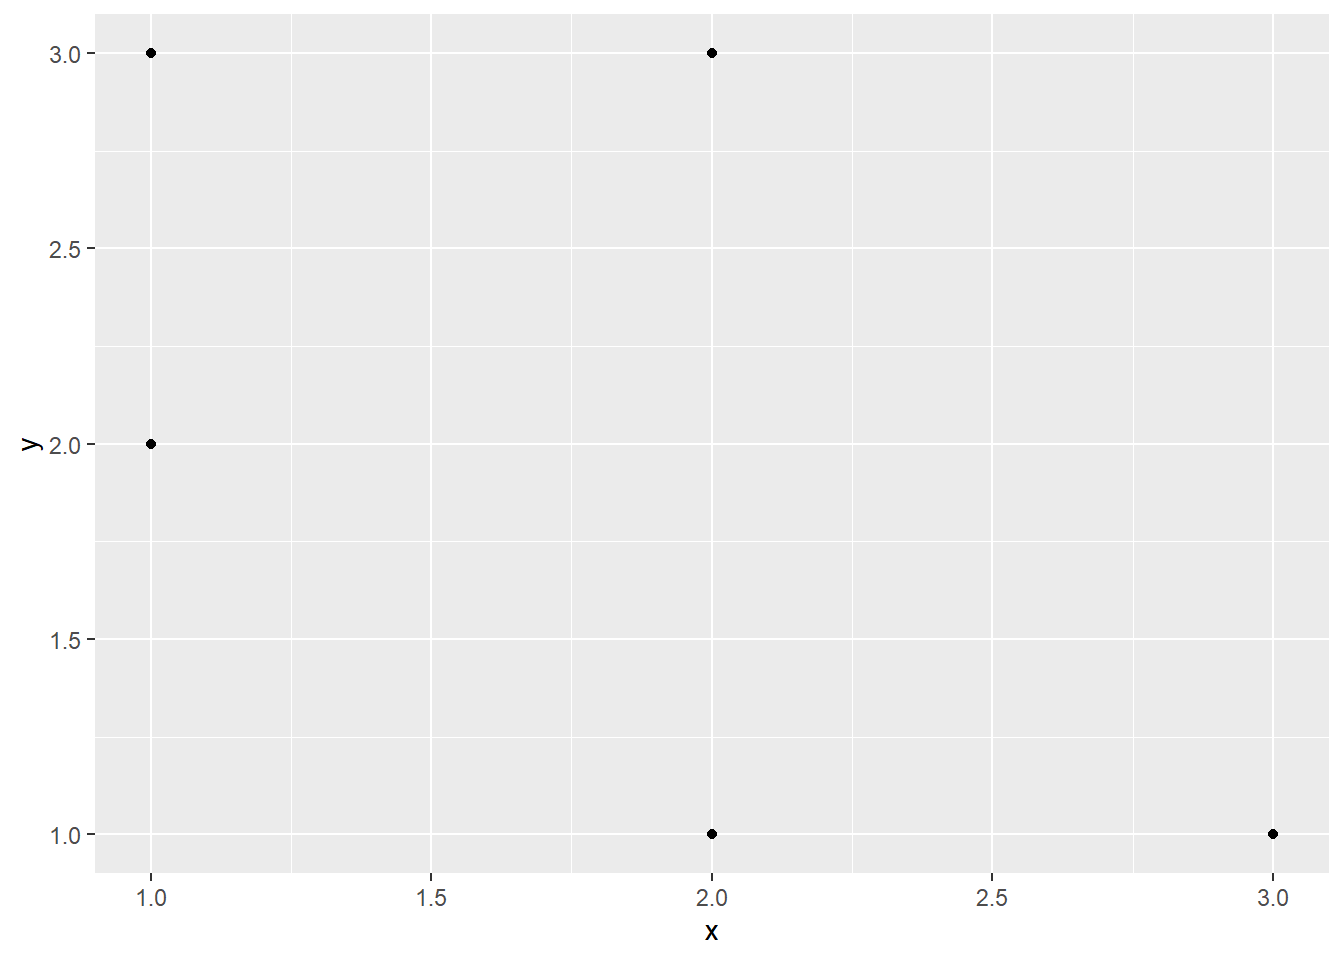
\includegraphics{ratrdsvs_files/figure-latex/unnamed-chunk-132-1.pdf}

We receive the \texttt{Warning:\ Removed\ 1\ rows\ containing\ missing\ values\ (geom\_point).}

In this case, its obvious that ggplot has had to get rid of the row of data with the \texttt{NA} value, and so we probably feel comfortable moving on with this warning. However, warnings can be a sign of something not behaving itself, and is usually a sign we should go back and double check our code. We might decide to move forward and ignore the warnings.

\hypertarget{trouble_errors}{%
\section{Common errors}\label{trouble_errors}}

There are a lot of common errors in R, that can usually be easily fixed\footnote{This section is nearly wholly stolen from \href{http://varianceexplained.org/courses/errors/}{David Robinson}}.

Errors mean that R has not been able to

\hypertarget{object-not-found.}{%
\subsection{Object not found.}\label{object-not-found.}}

Sometimes you might ask R to find something that doesn't exist, for example:

\begin{Shaded}
\begin{Highlighting}[]
\NormalTok{thing}
\end{Highlighting}
\end{Shaded}

\begin{itemize}
\tightlist
\item
  Error: object `thing' not found
\end{itemize}

The quote \texttt{Error:\ object\ \textquotesingle{}thing\textquotesingle{}\ not\ found} tells us that R can't find anything called `thing' in the environment, or any of the loaded packages.

\begin{itemize}
\item
  Check that you've loaded all your required packages
\item
  Make sure you're spelling `thing' right (and remember, R is case sensitive, `Thing' might be right)
\item
  Check you have definitely loaded all your datasets (if you're working in an R Markdown document you may have forgotten to run the line that tells R what `thing' is.)
\end{itemize}

\hypertarget{function-not-found}{%
\subsection{Function not found}\label{function-not-found}}

Similarly, sometimes you might an error telling you that a function doesn't exist.

\begin{Shaded}
\begin{Highlighting}[]
\KeywordTok{thing}\NormalTok{(}\DecValTok{1}\NormalTok{)}
\end{Highlighting}
\end{Shaded}

\begin{itemize}
\tightlist
\item
  Error in thing(1) : could not find function ``thing''
\end{itemize}

Again, you want to:

\begin{itemize}
\item
  Check you've definitely loaded the right packages
\item
  Make sure you're spelling `thing' right (remembering R is case sensitive\ldots{})
\item
  Make sure you definitely want to use a function. You can also get this error if you type \texttt{x\ (1\ /\ 2)}, even if you've predefined `x' as a value. R thinks that opening brackets usually means using a function, so if you want to perform the calculation \texttt{x\ *\ (1/2)} you need to include the \texttt{*} symbol.
\end{itemize}

\hypertarget{unexpected-symbols}{%
\subsection{Unexpected symbols}\label{unexpected-symbols}}

There are a few errors which are all similar, such as:

\begin{Shaded}
\begin{Highlighting}[]
\KeywordTok{mean}\NormalTok{(}\DecValTok{2}\NormalTok{,}\DecValTok{2}\NormalTok{,}\DecValTok{4}\NormalTok{,}\DecValTok{5}\NormalTok{,}\DecValTok{6}\NormalTok{)}\ErrorTok{)}
\end{Highlighting}
\end{Shaded}

\begin{itemize}
\tightlist
\item
  Error: unexpected `)' in ``mean(2,2,4,5,6))''
\end{itemize}

and

\begin{Shaded}
\begin{Highlighting}[]
\KeywordTok{mean}\NormalTok{(}\DecValTok{2}\NormalTok{,}\DecValTok{2}\NormalTok{,}\DecValTok{3}\NormalTok{,}\DecValTok{5} \DecValTok{6}\NormalTok{)}
\end{Highlighting}
\end{Shaded}

\begin{itemize}
\tightlist
\item
  Error: unexpected numeric constant in ``mean(2,2,3,5 6''
\end{itemize}

and

\begin{Shaded}
\begin{Highlighting}[]
\KeywordTok{mean}\NormalTok{(}\DecValTok{2}\NormalTok{,}\DecValTok{2}\NormalTok{,}\DecValTok{3}\NormalTok{;}\DecValTok{5}\NormalTok{,}\DecValTok{6}\NormalTok{)}
\end{Highlighting}
\end{Shaded}

\begin{itemize}
\tightlist
\item
  Error: unexpected `;' in ``mean(2,2,3;''
\end{itemize}

These are all clues to go back through the last run chunk of code and look for typos.

\hypertarget{quick-warnings-and-errors}{%
\section{Quick warnings and errors}\label{quick-warnings-and-errors}}

There is a great resource from \href{http://rex-analytics.com/decoding-error-messages-r/}{rex-analytics} on errors and warnings, which I'll display here:

\begin{figure}

{\centering 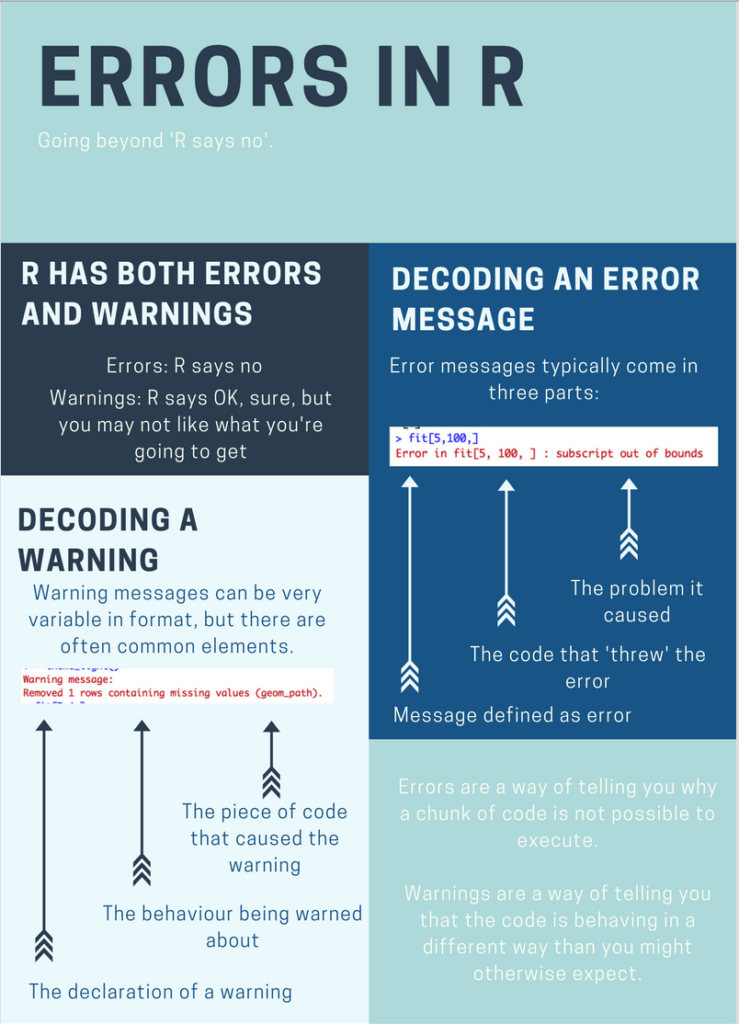
\includegraphics[width=10.26in]{images/08_troubleshooting/errors-in-R-739x1024} 

}

\caption{Rex-analytics great infographic on R warnings and errors}\label{fig:unnamed-chunk-138}
\end{figure}

\hypertarget{searching-for-help}{%
\section{Searching for help}\label{searching-for-help}}

Of course sometimes you can't figure out with what you already know. When this happens your next step is to google\footnote{or web search of your choice}.

Many, many people know that \href{https://dev.to/dvddpl/am-i-an-expert-developer-or-just-an-expert-googler-4390}{they should just google things}. These people have it cracked. If you know how to find an answer on Google, you will be immediately more employable than the person who doesn't.

This has even become a meme . . .

\begin{figure}

{\centering 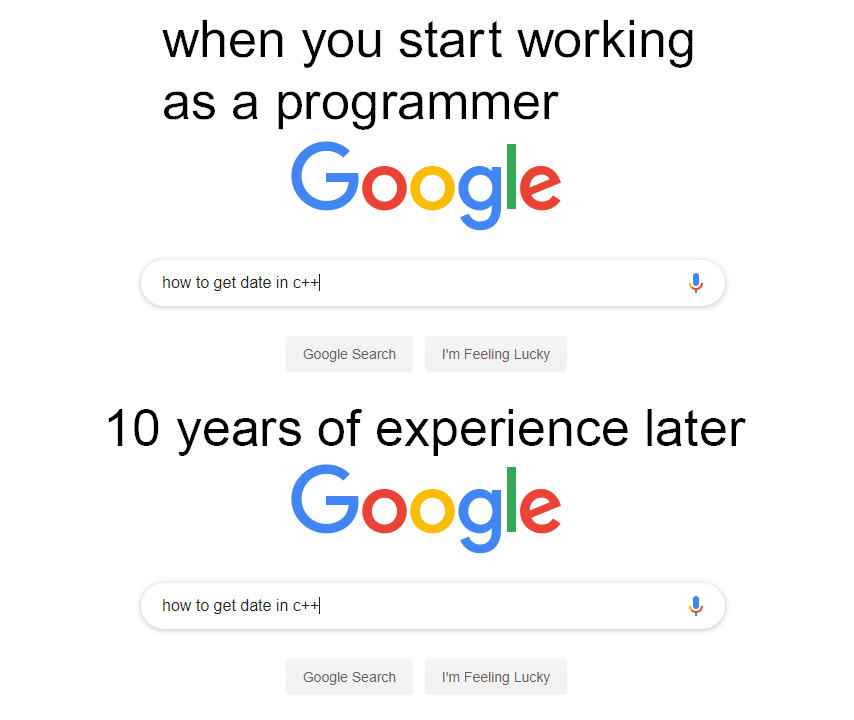
\includegraphics[width=11.86in]{images/08_troubleshooting/meme1} 

}

\caption{10 years of programming, stolen from /r/programmerhumor}\label{fig:unnamed-chunk-139}
\end{figure}

Quite a few memes actually . . .

\begin{figure}

{\centering 
\includegraphics[width=6.94in]{images/08_troubleshooting/meme2} 

}

\caption{Jerry gets rewarded for googling, stolen from /r/programmerhumor}\label{fig:unnamed-chunk-140}
\end{figure}

One more to make the point . . .

\begin{figure}

{\centering 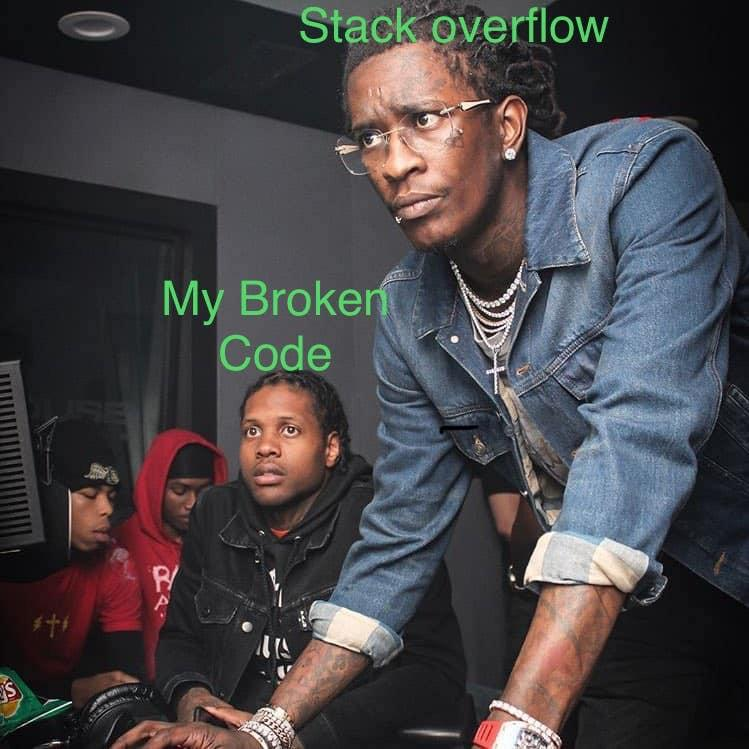
\includegraphics[width=10.4in]{images/08_troubleshooting/meme3} 

}

\caption{Young Thug knows how to google, stolen from /r/programmerhumor}\label{fig:unnamed-chunk-141}
\end{figure}

The first step is to copy your error message and paste it into google.

Scroll through the answers until you see one that looks similar to yours.

Depending on how complex your code is, this might not be as simple as it seems. You may need to look at your error message for the key components.

More often than not, you will probably find yourself on \href{https://stackoverflow.com/}{stackoverflow}. I have \href{https://stackoverflow.com/questions/56036568/how-to-use-fct-relevel-with-mutate-at-syntax}{personally asked questions on there}. Lots of people make it their hobby to sit on stackoverflow and help people with their code. Sometimes you might find that the writer of the package you're working with \href{https://stackoverflow.com/questions/50375791/passing-top-n-and-arrange-to-ggplot-dplyr}{takes the time to answer}.

When you start to ask a question on stackoverflow, it gives you a really helpful set of tips. I have often started to write an answer and by the time I've worked through stackoverflow's tips, I've figured out the answer.

\hypertarget{trouble_help}{%
\subsection{Tips for asking for help}\label{trouble_help}}

\begin{enumerate}
\def\labelenumi{\arabic{enumi}.}
\tightlist
\item
  Summarise the problem
\end{enumerate}

\begin{verbatim}
* What are you trying to do (what's your ideal output?)

* What is happening at the moment (what's going wrong?)

* What errors/warnings is R giving you?
\end{verbatim}

\begin{enumerate}
\def\labelenumi{\arabic{enumi}.}
\setcounter{enumi}{1}
\tightlist
\item
  Describe what you've tried
\end{enumerate}

\begin{verbatim}
* What different methods have you tried? (Hint: if you haven't tried anything it's going to annoy people)

* Why do you think your attempts haven't worked?
\end{verbatim}

\begin{enumerate}
\def\labelenumi{\arabic{enumi}.}
\setcounter{enumi}{2}
\tightlist
\item
  Show some code
\end{enumerate}

\begin{verbatim}
* Share a minimum reproducible example (reprex) so people can tell exactly what you're trying. 
\end{verbatim}

Even if you don't want to ask your question on stackoverflow, these tips can be really useful.

\hypertarget{trouble_reprex}{%
\section{Reproducible Examples (reprex)}\label{trouble_reprex}}

I've talked a lot about reproducible examples or reprexes. Again, stackoverflow \href{https://stackoverflow.com/help/minimal-reproducible-example}{has great guidance on creating one of these}. But we've actually already made one of these all the way back in \protect\hyperlink{ex_createdata}{chapter three} when we were trying to figure out why \texttt{summary} was treating characters different from numerical variables.

There are three key elements of a reprex:

\begin{enumerate}
\def\labelenumi{\arabic{enumi}.}
\item
  Be minimal
  * Use as little code as possible to reproduce the problem
  * You can do this in two main ways:

  \begin{itemize}
  \tightlist
  \item
    Create a new file and add only what you need to reproduce the problem
  \item
    Remove code bit by bit from your file until you find the part that isn't working
  \item
    In reprexes its often very useful to test on an inbuilt dataset in R, such as \texttt{mpg} or \texttt{cars}, because we all have access to these datasets, and it means you don't have to send big data files to anyone (particularly if you're working on data that shouldn't be shared, e.g.~personal data)
  \end{itemize}
\item
  Make sure your question is complete when you send it to someone
  * It sounds daft, but this happens more than you think.
  * The person trying to solve your problem should be able to replicate it using your code
  * Its a good idea to restart your R session, clear your environment, and run all your code fresh to check the problem still exists before sending it along.
  * Oh - and always send the actual code. Screenshots are not useful
\item
  Describe the problem again before sending it
  * You may be surprised at how the problem has changed while troubleshooting!
\end{enumerate}

\hypertarget{statsbasic}{%
\chapter{Basic Statistics}\label{statsbasic}}

\begin{los}
You can skip this chapter if \ldots{}

\begin{itemize}
\item
  You can identify some common descriptive statistics
\item
  You can report descriptive statistics
\item
  You can describe the statistical formula for the mean and standard
  deviation
\end{itemize}
\end{los}

\hypertarget{descstats}{%
\section{Descriptive stats}\label{descstats}}

Descriptive statistics, unsurprisingly, \textbf{describe} the data. But why do we need to describe data?

Imagine that we had a field of cows.

\begin{figure}

{\centering 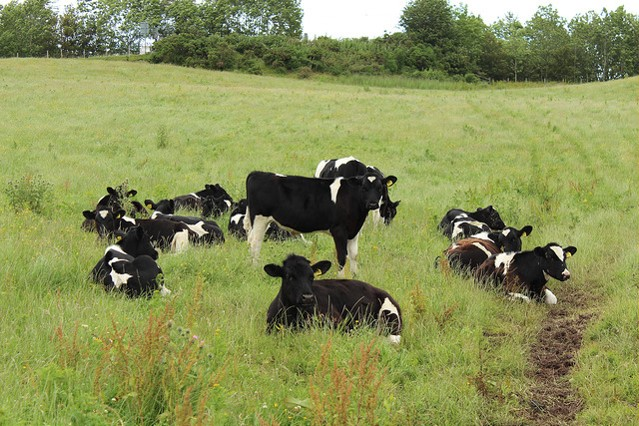
\includegraphics[width=8.88in]{images/09_statbasic/cows_1} 

}

\caption{A field of heifers}\label{fig:unnamed-chunk-143}
\end{figure}

We know that the first heifer has a weight of 211.3kg

\begin{figure}

{\centering 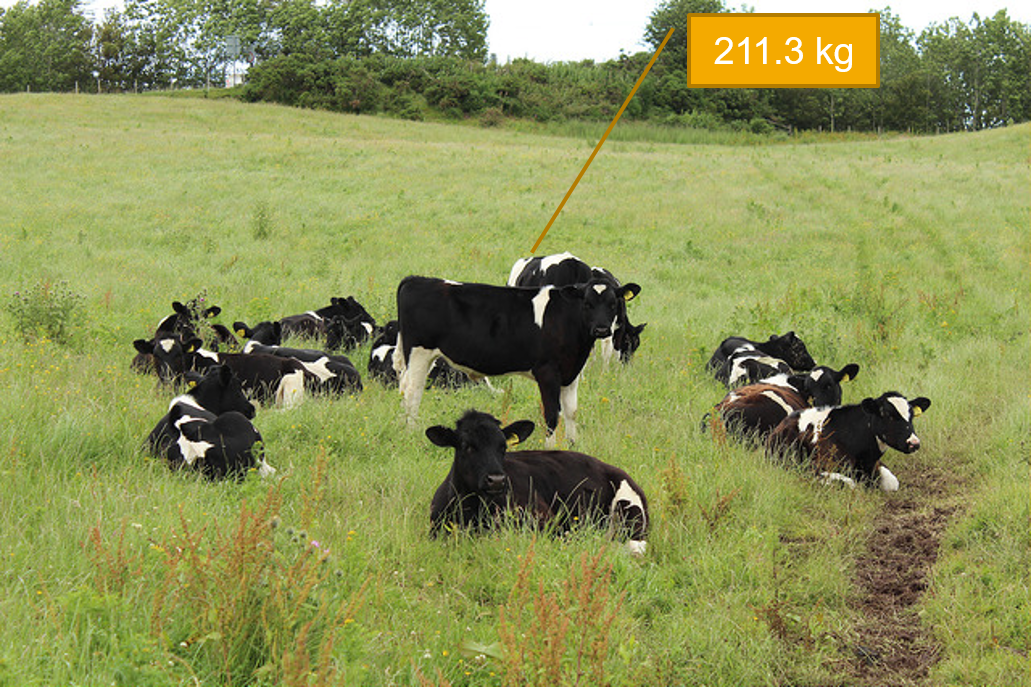
\includegraphics[width=14.32in]{images/09_statbasic/cows_2} 

}

\caption{A field of heifers, 1 weight known}\label{fig:unnamed-chunk-144}
\end{figure}

And that the second heifer has a weight of 200.4kg

\begin{figure}

{\centering \includegraphics[width=14.32in]{images/09_statbasic/cows_3} 

}

\caption{A field of heifers, 2 weights known}\label{fig:unnamed-chunk-145}
\end{figure}

We can keep going, recording weights for every cow until we know all of them.

\begin{figure}

{\centering \includegraphics[width=22.28in]{images/09_statbasic/cows_4} 

}

\caption{A field of heifers, all weights known}\label{fig:unnamed-chunk-146}
\end{figure}

They say that knowledge is power, and so now we know the weights of all these cows, we should be able to make better choices. Unfortunately, we often can't make choices on an individual basis, so we need to make a choice that suits the most cows. How can we condense this information down?

Statistics is really just condensing the real world down into simpler mathematical descriptions.

\hypertarget{mathematical-notation}{%
\subsection{Mathematical notation}\label{mathematical-notation}}

I've changed my mind several times about whether I should teach mathematical notation when talking about statistics. I've decided to include it in this chapter, but if you find yourself glazing over, don't worry too much. Sometimes I don't bother teaching this.

I've made the decision to talk about it because fundamentally, understanding \textbf{what} is happening when you calculate a mean (or a standard deviation) can help you understand some of the more complicated parts of statistics. You will likely never be quizzed on this, so I wouldn't try to memorise them, but they can be a useful thing to know.

\hypertarget{general-notation}{%
\subsubsection{General notation}\label{general-notation}}

Generally, in mathematical notation:

\begin{itemize}
\item
  Upper case letters denote a variable name (\(X\), \(Y\), \(Z\) \ldots{})
\item
  Lower case letters denote a specific value of the variable (\(x\), \(y\), \(z\) \ldots{})
\item
  Sample data is indicated with lower case letters (\(v\)\{\(x_1\), \(x_2\) \ldots{} \(x_n\)\})
\end{itemize}

So in this example we might say \emph{Let heifer weight be \(X\)}.

\hypertarget{stats_mean}{%
\subsection{The mean}\label{stats_mean}}

Let's create a dataset of heifer weight:

\begin{Shaded}
\begin{Highlighting}[]
\NormalTok{coos <-}\StringTok{ }\KeywordTok{tibble}\NormalTok{(}\DataTypeTok{heifer_id =} \KeywordTok{c}\NormalTok{(}\DecValTok{1}\NormalTok{, }\DecValTok{2}\NormalTok{, }\DecValTok{3}\NormalTok{, }\DecValTok{4}\NormalTok{, }\DecValTok{5}\NormalTok{, }\DecValTok{6}\NormalTok{, }\DecValTok{7}\NormalTok{, }\DecValTok{8}\NormalTok{, }\DecValTok{9}\NormalTok{, }\DecValTok{10}\NormalTok{, }\DecValTok{11}\NormalTok{, }\DecValTok{12}\NormalTok{),}
               \DataTypeTok{weight =} \KeywordTok{c}\NormalTok{(}\FloatTok{211.3}\NormalTok{, }\FloatTok{200.4}\NormalTok{, }\FloatTok{220.1}\NormalTok{, }\FloatTok{200.8}\NormalTok{, }\FloatTok{222.0}\NormalTok{, }\FloatTok{209.3}\NormalTok{, }
                          \FloatTok{195.8}\NormalTok{, }\FloatTok{220.4}\NormalTok{, }\FloatTok{225.2}\NormalTok{, }\FloatTok{218.7}\NormalTok{, }\FloatTok{193.7}\NormalTok{, }\FloatTok{209.7}\NormalTok{))}
\end{Highlighting}
\end{Shaded}

We always want to visualise our data first - but just knowing weight isn't that interesting:

\begin{Shaded}
\begin{Highlighting}[]
\NormalTok{coos }\OperatorTok\StringTok{ }
\StringTok{  }\KeywordTok{ggplot}\NormalTok{(}\KeywordTok{aes}\NormalTok{(}\DataTypeTok{x =}\NormalTok{ heifer_id, }\DataTypeTok{y =}\NormalTok{ weight, }\DataTypeTok{colour =} \KeywordTok{as.factor}\NormalTok{(heifer_id))) }\OperatorTok{+}
\StringTok{  }\KeywordTok{geom_point}\NormalTok{() }\OperatorTok{+}
\StringTok{  }\KeywordTok{scale_y_continuous}\NormalTok{(}\DataTypeTok{limits =} \KeywordTok{c}\NormalTok{(}\DecValTok{0}\NormalTok{, }\DecValTok{250}\NormalTok{)) }\OperatorTok{+}
\StringTok{  }\KeywordTok{scale_x_continuous}\NormalTok{(}\DataTypeTok{limits =} \KeywordTok{c}\NormalTok{(}\DecValTok{0}\NormalTok{,}\DecValTok{12}\NormalTok{), }\DataTypeTok{breaks =} \KeywordTok{seq}\NormalTok{(}\DecValTok{0}\NormalTok{,}\DecValTok{12}\NormalTok{,}\DecValTok{1}\NormalTok{)) }\OperatorTok{+}
\StringTok{  }\KeywordTok{theme_classic}\NormalTok{() }\OperatorTok{+}
\StringTok{  }\KeywordTok{theme}\NormalTok{(}\DataTypeTok{legend.position =} \StringTok{"none"}\NormalTok{) }\OperatorTok{+}
\StringTok{  }\KeywordTok{labs}\NormalTok{(}\DataTypeTok{y =} \StringTok{"Weight (kg)"}\NormalTok{,}
       \DataTypeTok{x =} \StringTok{"Heifer ID"}\NormalTok{)}
\end{Highlighting}
\end{Shaded}

\begin{figure}

{\centering \includegraphics{ratrdsvs_files/figure-latex/unnamed-chunk-148-1} 

}

\caption{Weight (kg) of 12 heifers}\label{fig:unnamed-chunk-148}
\end{figure}

There's not much that we can say about this chart. Most heifers seem to weigh around 207kg. But that's an estimate that comes from me just eyeballing the data. We could draw a line at around 207kg, a line of best fit, which is a rough guess that tries to minimise the amount of distance between the line and each point.

\begin{Shaded}
\begin{Highlighting}[]
\NormalTok{coos }\OperatorTok\StringTok{ }
\StringTok{  }\KeywordTok{ggplot}\NormalTok{(}\KeywordTok{aes}\NormalTok{(}\DataTypeTok{x =}\NormalTok{ heifer_id, }\DataTypeTok{y =}\NormalTok{ weight, }\DataTypeTok{colour =} \KeywordTok{as.factor}\NormalTok{(heifer_id))) }\OperatorTok{+}
\StringTok{  }\KeywordTok{geom_point}\NormalTok{() }\OperatorTok{+}
\StringTok{  }\KeywordTok{scale_y_continuous}\NormalTok{(}\DataTypeTok{limits =} \KeywordTok{c}\NormalTok{(}\DecValTok{0}\NormalTok{, }\DecValTok{250}\NormalTok{)) }\OperatorTok{+}
\StringTok{  }\KeywordTok{scale_x_continuous}\NormalTok{(}\DataTypeTok{limits =} \KeywordTok{c}\NormalTok{(}\DecValTok{0}\NormalTok{,}\DecValTok{12}\NormalTok{), }\DataTypeTok{breaks =} \KeywordTok{seq}\NormalTok{(}\DecValTok{0}\NormalTok{,}\DecValTok{12}\NormalTok{,}\DecValTok{1}\NormalTok{)) }\OperatorTok{+}
\StringTok{  }\KeywordTok{theme_classic}\NormalTok{() }\OperatorTok{+}
\StringTok{  }\KeywordTok{theme}\NormalTok{(}\DataTypeTok{legend.position =} \StringTok{"none"}\NormalTok{) }\OperatorTok{+}
\StringTok{  }\KeywordTok{labs}\NormalTok{(}\DataTypeTok{y =} \StringTok{"Weight (kg)"}\NormalTok{,}
       \DataTypeTok{x =} \StringTok{"Heifer ID"}\NormalTok{) }\OperatorTok{+}
\StringTok{  }\KeywordTok{geom_segment}\NormalTok{(}\DataTypeTok{x =} \DecValTok{0}\NormalTok{, }\DataTypeTok{xend =} \DecValTok{12}\NormalTok{, }\DataTypeTok{y =} \DecValTok{207}\NormalTok{, }\DataTypeTok{yend =} \DecValTok{207}\NormalTok{)}
\end{Highlighting}
\end{Shaded}

\begin{figure}

{\centering \includegraphics{ratrdsvs_files/figure-latex/unnamed-chunk-149-1} 

}

\caption{Weight (kg) of 12 heifers, with a human-estimated best fit line}\label{fig:unnamed-chunk-149}
\end{figure}

We could use maths to draw that line in a better place . . .

If we add up all the values of weight and divide by the number of cows . . .

\begin{Shaded}
\begin{Highlighting}[]
\KeywordTok{sum}\NormalTok{(coos}\OperatorTok{$}\NormalTok{weight) }\OperatorTok{/}\StringTok{ }\DecValTok{12}
\end{Highlighting}
\end{Shaded}

\begin{verbatim}
## [1] 210.6167
\end{verbatim}

We get the exact same value as if we asked R to calculate the mean directly (using the handy \protect\hyperlink{tidy_summ}{\texttt{summarise} function}):

\begin{Shaded}
\begin{Highlighting}[]
\NormalTok{coos }\OperatorTok\StringTok{ }
\StringTok{  }\KeywordTok{summarise}\NormalTok{(}\KeywordTok{mean}\NormalTok{(weight))}
\end{Highlighting}
\end{Shaded}

\begin{verbatim}
## # A tibble: 1 x 1
##   `mean(weight)`
##            <dbl>
## 1           211.
\end{verbatim}

\hypertarget{notation-of-the-mean}{%
\subsubsection{Notation of the mean}\label{notation-of-the-mean}}

We all know how to calculate the mean, but what does that look like in mathematical notation?

The equation for the mean is:

\[\overline{x} = \frac{\sum x^i}{n}    \]

\begin{translate}
Let's break this equation down:

\begin{itemize}
\item
  \(\overline{x}\) is the mean of the sample
\item
  \(\sum\), the greek letter \textbf{sigma} means `add all this
  together'
\item
  \(x^i\) means `every data point in sample'
\item
  \(n\) means `number of observations in sample'.
\end{itemize}
\end{translate}
\begin{figure}

{\centering \includegraphics{images/09_statbasic/notation_mean} 

}

\caption{Formula for the mean}\label{fig:unnamed-chunk-153}
\end{figure}

\hypertarget{the-mean-as-a-model}{%
\subsection{The mean as a model}\label{the-mean-as-a-model}}

So now we know that \(\overline{x}\) = 210.6kg. We have created an imaginary \textbf{model} cow. This model cow has a weight of 210.6kg, and we know that she is not exactly real, but we can choose to make use of her, because she has a little bit of information from all of the samples.

\begin{figure}

{\centering \includegraphics[width=4.88in]{images/09_statbasic/meancow} 

}

\caption{The mean cow}\label{fig:unnamed-chunk-154}
\end{figure}

\hypertarget{stats_median}{%
\section{Median}\label{stats_median}}

There are other imagniary cows we could build to represent our dataset.

\begin{Shaded}
\begin{Highlighting}[]
\NormalTok{coos }\OperatorTok\StringTok{ }
\StringTok{  }\KeywordTok{ggplot}\NormalTok{(}\KeywordTok{aes}\NormalTok{(}\DataTypeTok{y =}\NormalTok{ weight)) }\OperatorTok{+}
\StringTok{  }\KeywordTok{geom_boxplot}\NormalTok{() }\OperatorTok{+}
\StringTok{  }\KeywordTok{theme_classic}\NormalTok{() }\OperatorTok{+}
\StringTok{  }\KeywordTok{theme}\NormalTok{(}\DataTypeTok{legend.position =} \StringTok{"none"}\NormalTok{) }\OperatorTok{+}
\StringTok{  }\KeywordTok{labs}\NormalTok{(}\DataTypeTok{y =} \StringTok{"Weight (kg)"}\NormalTok{)}
\end{Highlighting}
\end{Shaded}

\begin{figure}

{\centering \includegraphics{ratrdsvs_files/figure-latex/unnamed-chunk-155-1} 

}

\caption{Weight (kg) distribution of 12 heifers}\label{fig:unnamed-chunk-155}
\end{figure}

The thick middle line in this boxplot represents the \textbf{median} cow.

\begin{figure}

{\centering \includegraphics[width=4.75in]{images/09_statbasic/mediancow} 

}

\caption{The median cow}\label{fig:unnamed-chunk-156}
\end{figure}

Now the formula for the median is a little more complicated than I want to get into here, but the median essentially puts all of the cows in order:

\begin{Shaded}
\begin{Highlighting}[]
\NormalTok{coos }\OperatorTok\StringTok{ }
\StringTok{  }\KeywordTok{arrange}\NormalTok{(weight)}
\end{Highlighting}
\end{Shaded}

\begin{verbatim}
## # A tibble: 12 x 2
##    heifer_id weight
##        <dbl>  <dbl>
##  1        11   194.
##  2         7   196.
##  3         2   200.
##  4         4   201.
##  5         6   209.
##  6        12   210.
##  7         1   211.
##  8        10   219.
##  9         3   220.
## 10         8   220.
## 11         5   222 
## 12         9   225.
\end{verbatim}

And then we pick the middle value. We have 12 cows, so our two middle values are 209.7 and 211.3. So to find the median, we add those two values together and divide by 2.

\begin{Shaded}
\begin{Highlighting}[]
\NormalTok{coos }\OperatorTok\StringTok{ }
\StringTok{  }\KeywordTok{summarise}\NormalTok{(}\DataTypeTok{median_weight =} \KeywordTok{median}\NormalTok{(weight))}
\end{Highlighting}
\end{Shaded}

\begin{verbatim}
## # A tibble: 1 x 1
##   median_weight
##           <dbl>
## 1          210.
\end{verbatim}

\hypertarget{stats_mode}{%
\section{Mode}\label{stats_mode}}

The final simple model we will talk about is the \textbf{mode}, or the most frequent value in a dataset. The mode isn't that useful, and so there isn't actually an inbuilt function to visualise or calculate it.

\begin{Shaded}
\begin{Highlighting}[]
\NormalTok{mode <-}\StringTok{ }\ControlFlowTok{function}\NormalTok{(v) \{}
\NormalTok{   uniqv <-}\StringTok{ }\KeywordTok{unique}\NormalTok{(v)}
\NormalTok{   uniqv[}\KeywordTok{which.max}\NormalTok{(}\KeywordTok{tabulate}\NormalTok{(}\KeywordTok{match}\NormalTok{(v, uniqv)))]}
\NormalTok{\}}

\NormalTok{coos }\OperatorTok\StringTok{ }
\StringTok{  }\KeywordTok{summarise}\NormalTok{(}\DataTypeTok{mode_weight=}\NormalTok{ (}\KeywordTok{mode}\NormalTok{(weight)))}
\end{Highlighting}
\end{Shaded}

\begin{verbatim}
## # A tibble: 1 x 1
##   mode_weight
##         <dbl>
## 1        211.
\end{verbatim}

The mode is a bit . . . useless . . . but it is still a model cow, so it also gets its own picture in this example.

\begin{figure}

{\centering \includegraphics[width=5.5in]{images/09_statbasic/modecow} 

}

\caption{The modal cow}\label{fig:unnamed-chunk-160}
\end{figure}

\hypertarget{stats_which}{%
\section{Which model?}\label{stats_which}}

The mean, mode and median cow all try to give a good approximation of \textbf{most} cows in our field. We know that they can't describe every cow in detail (because we don't want to have to learn every single cow's weight off by heart), but they all have to lose important information.

With each of these models - we hope that our calculated weight is close to most of the population. We know that there is always natural variation in the world, and some cows might be very heavy, and some cows might be very thin, but our hope is that our models are fair representations of \textbf{most} cows in our dataset. But each model takes a different approach to this.

The mean is also described as the central tendency, and it takes into account every single individual in the sample. However, if you have a very skinny or very heavy cow, they will (by virtue of how the mean is calcualted) have a big impact on the final value.

The median takes the `middle' value of the dataset, and can be very useful when you have extreme \textbf{outliers} in a dataset, because it essentially ignores those values. The median is sometimes referred to as the most resilient statistic because so long as at least 50\% of your values are normal, the median will be close to at least 50\% of your individuals.

The mode, as the most common value in the dataset, but this is rarely very useful in biological data. What if we had two very small cows who weighed 100kg, and every other cow of normal weight had a unique value? The mode would make its imaginary cow 100kg, even though every other cow in the dataset was over 100kg heavier. However, you can use the mode for nominal data, which can be useful, e.g.~what is the most common name of cow?

\hypertarget{stats_variation}{%
\section{Measures of variation}\label{stats_variation}}

In the previous section we talked about outliers, and how they can affect these three models of our cows.

We've already \protect\hyperlink{vis_hist}{looked at ways to visualise distributions}, but lets remind ourselves:

\begin{Shaded}
\begin{Highlighting}[]
\NormalTok{coos }\OperatorTok\StringTok{ }
\StringTok{  }\KeywordTok{ggplot}\NormalTok{(}\KeywordTok{aes}\NormalTok{(}\DataTypeTok{x =}\NormalTok{ weight)) }\OperatorTok{+}
\StringTok{  }\KeywordTok{geom_histogram}\NormalTok{(}\DataTypeTok{binwidth =} \DecValTok{10}\NormalTok{) }\OperatorTok{+}
\StringTok{  }\KeywordTok{theme_classic}\NormalTok{()}
\end{Highlighting}
\end{Shaded}

\begin{figure}

{\centering \includegraphics{ratrdsvs_files/figure-latex/unnamed-chunk-161-1} 

}

\caption{A histogram of heifer weight}\label{fig:unnamed-chunk-161}
\end{figure}

The histogram shows us how many cows are in each weight category (or `bin'). We can overlay the mean, median and mode on this, to see which one gets closest to the `middle'.

\begin{Shaded}
\begin{Highlighting}[]
\NormalTok{coos }\OperatorTok\StringTok{ }
\StringTok{  }\KeywordTok{ggplot}\NormalTok{(}\KeywordTok{aes}\NormalTok{(}\DataTypeTok{x =}\NormalTok{ weight)) }\OperatorTok{+}
\StringTok{  }\KeywordTok{geom_histogram}\NormalTok{(}\DataTypeTok{binwidth =} \DecValTok{10}\NormalTok{) }\OperatorTok{+}
\StringTok{  }\KeywordTok{theme_classic}\NormalTok{() }\OperatorTok{+}
\StringTok{  }\KeywordTok{geom_segment}\NormalTok{(}\DataTypeTok{x =} \FloatTok{210.6}\NormalTok{, }\DataTypeTok{xend =} \FloatTok{210.6}\NormalTok{, }\DataTypeTok{y =} \DecValTok{0}\NormalTok{, }\DataTypeTok{yend =} \DecValTok{4}\NormalTok{, }\DataTypeTok{colour =} \StringTok{"pink2"}\NormalTok{) }\OperatorTok{+}
\StringTok{  }\KeywordTok{geom_segment}\NormalTok{(}\DataTypeTok{x =} \FloatTok{210.5}\NormalTok{, }\DataTypeTok{xend =} \FloatTok{210.5}\NormalTok{, }\DataTypeTok{y =} \DecValTok{0}\NormalTok{, }\DataTypeTok{yend =} \FloatTok{3.5}\NormalTok{, }\DataTypeTok{colour =} \StringTok{"yellow1"}\NormalTok{) }\OperatorTok{+}
\StringTok{  }\KeywordTok{geom_segment}\NormalTok{(}\DataTypeTok{x =} \FloatTok{211.3}\NormalTok{, }\DataTypeTok{xend =} \FloatTok{211.3}\NormalTok{, }\DataTypeTok{y =} \DecValTok{0}\NormalTok{, }\DataTypeTok{yend =} \DecValTok{4}\NormalTok{, }\DataTypeTok{colour =} \StringTok{"lightblue1"}\NormalTok{)}
\end{Highlighting}
\end{Shaded}

\begin{figure}

{\centering \includegraphics{ratrdsvs_files/figure-latex/unnamed-chunk-162-1} 

}

\caption{A histogram of heifer weight(kg), mean, median and mode shown}\label{fig:unnamed-chunk-162}
\end{figure}

Now these three lines (the median (yellow), mean (pink) and mode (blue)) are all very close to one another. So close in fact that the mean and median are nearly on top of one another. This suggests to us that our field of heifers is fairly \textbf{normal}. Most observations are around the mean, and so the mean and the median are fairly similar. We have very few unusual observations (very few underweight or overweight cows).

Again, this is just us eyeballing the data. It can be useful to put numbers on how variable a dataset is.

\hypertarget{stats_variance}{%
\subsection{Variance}\label{stats_variance}}

Variance (\(\sigma^2\)) describes how far away each observation in our sample is from the sample mean.

If we drew a line representing the mean (\(\overline{x}\)) on our scatteplot of each individual value, we could measure how far away each point was from the line. If we added all these numbers together they would sum to zero (if you want to see a proof of this \protect\hyperlink{stats_proofvariance}{jump here}).

\begin{Shaded}
\begin{Highlighting}[]
\NormalTok{coos }\OperatorTok\StringTok{ }
\StringTok{  }\KeywordTok{ggplot}\NormalTok{(}\KeywordTok{aes}\NormalTok{(}\DataTypeTok{x =}\NormalTok{ heifer_id, }\DataTypeTok{y =}\NormalTok{ weight, }\DataTypeTok{colour =} \KeywordTok{as.factor}\NormalTok{(heifer_id))) }\OperatorTok{+}
\StringTok{  }\KeywordTok{geom_point}\NormalTok{() }\OperatorTok{+}
\StringTok{  }\KeywordTok{scale_y_continuous}\NormalTok{(}\DataTypeTok{limits =} \KeywordTok{c}\NormalTok{(}\DecValTok{0}\NormalTok{, }\DecValTok{250}\NormalTok{)) }\OperatorTok{+}
\StringTok{  }\KeywordTok{scale_x_continuous}\NormalTok{(}\DataTypeTok{limits =} \KeywordTok{c}\NormalTok{(}\DecValTok{0}\NormalTok{,}\DecValTok{12}\NormalTok{), }\DataTypeTok{breaks =} \KeywordTok{seq}\NormalTok{(}\DecValTok{0}\NormalTok{,}\DecValTok{12}\NormalTok{,}\DecValTok{1}\NormalTok{)) }\OperatorTok{+}
\StringTok{  }\KeywordTok{theme_classic}\NormalTok{() }\OperatorTok{+}
\StringTok{  }\KeywordTok{theme}\NormalTok{(}\DataTypeTok{legend.position =} \StringTok{"none"}\NormalTok{) }\OperatorTok{+}
\StringTok{  }\KeywordTok{labs}\NormalTok{(}\DataTypeTok{y =} \StringTok{"Weight (kg)"}\NormalTok{,}
       \DataTypeTok{x =} \StringTok{"Heifer ID"}\NormalTok{) }\OperatorTok{+}
\StringTok{  }\KeywordTok{geom_segment}\NormalTok{(}\DataTypeTok{x =} \DecValTok{0}\NormalTok{, }\DataTypeTok{xend =} \DecValTok{12}\NormalTok{, }\DataTypeTok{y =} \FloatTok{210.6}\NormalTok{, }\DataTypeTok{yend =} \FloatTok{210.6}\NormalTok{, }\DataTypeTok{colour =} \StringTok{"pink2"}\NormalTok{)}
\end{Highlighting}
\end{Shaded}

\begin{figure}

{\centering \includegraphics{ratrdsvs_files/figure-latex/unnamed-chunk-163-1} 

}

\caption{Weight (kg) of 12 heifers, with a mean line}\label{fig:unnamed-chunk-163}
\end{figure}

So we need to transform the distances by squaring them. Now, if we were dealing with hundreds of observations we would of course have a much bigger number, so we need to standardise them by the number of observations (just like we do with the mean calculation).

We can calculate the variance of the cows' weight very easily:

\begin{Shaded}
\begin{Highlighting}[]
\NormalTok{coos }\OperatorTok\StringTok{ }
\StringTok{  }\KeywordTok{summarise}\NormalTok{(}\DataTypeTok{variance =} \KeywordTok{var}\NormalTok{(weight))}
\end{Highlighting}
\end{Shaded}

\begin{verbatim}
## # A tibble: 1 x 1
##   variance
##      <dbl>
## 1     118.
\end{verbatim}

\hypertarget{formula-for-variance}{%
\subsubsection{Formula for variance}\label{formula-for-variance}}

Variance is calculated like this:

\[\sigma^2 = \frac{\sum(x-\overline{x})^2}{n-1} \]

\begin{translate}
Breaking this equation down \ldots{}

\begin{itemize}
\item
  \(\sigma^2\) is the symbol for variance
\item
  \(\sum(x-\overline{x})^2\) means 'take each value of \(x\) and
  subtract the mean (\(\overline{x\)\}). Square this value (\(^2\)) and
  add them all together (\(\sum\))
\item
  Divide this value by the total number in the sample, minus 1
  (\(n-1\)). We say \(n-1\) because we are estimating the variance of a
  sample population\footnote{Why is n-1 you may ask? The short answer is
    that this is called the
    \href{https://en.wikipedia.org/wiki/Bessel\%27s_correction}{Bessel's
    Correction} and I'm happy to talk about it with you, but this
    chapter's long enough as it is.}
\end{itemize}
\end{translate}

\hypertarget{stats_sd}{%
\subsection{Standard Deviation}\label{stats_sd}}

The standard deviation (\(\sigma\)) is very similar to variance (\(\sigma^2\)). Can you guess what the difference is?

The standard deviation is the square root of the variance. When we calculate the variance, we simply sum all the squares together, but we really want to express this number in the same unit as the original measurements (not the square of the measurements). So if we take the square root of the variance, we calculated the standard deviation. This makes the standard deviation a really useful add-on to the mean, because its expressed in the same units.

We can of course calculate this:

\begin{Shaded}
\begin{Highlighting}[]
\NormalTok{coos }\OperatorTok\StringTok{ }
\StringTok{  }\KeywordTok{summarise}\NormalTok{(}\DataTypeTok{standard_deviation =} \KeywordTok{sd}\NormalTok{(weight))}
\end{Highlighting}
\end{Shaded}

\begin{verbatim}
## # A tibble: 1 x 1
##   standard_deviation
##                <dbl>
## 1               10.9
\end{verbatim}

\hypertarget{formula-for-standard-deviation.}{%
\subsubsection{Formula for standard deviation.}\label{formula-for-standard-deviation.}}

\[\sigma = \sqrt \frac{\sum(x-\overline{x})^2}{n-1} \]

\begin{translate}
Breaking this equation down \ldots{}

\begin{itemize}
\item
  \(\sigma\) is the symbol for standard deviation
\item
  \(\sum(x-\overline{x})^2\) means 'take each value of \(x\) and
  subtract the mean (\(\overline{x\)\}). Square this value (\(^2\)) and
  add them all together (\(\sum\))
\item
  Divide this value by the total number in the sample, minus 1 (\(n-1\))
\item
  Take the square root (\(\sqrt\)) of this value.
\end{itemize}
\end{translate}

\hypertarget{stats_se}{%
\subsection{Standard Error}\label{stats_se}}

The third and final measure of variance I'll discuss in this chapter is the \textbf{standard error} (\(\sigma_\overline{x}\)).

The standard error is an attempt to describe how far away the sample mean (\(\overline{x}\)) is from the true population mean (\(\mu\))?

In our cows example, we've measured 12 cows, but we know this is not all the cows in the world. If, in theory, we could measure every single cow in the world, we could calculate the variance of the population (we wouldn't need to say \((n-1)\) in our variance calculation because we would know exactly how many cows we had).

\[\sigma_{population} = \sqrt \frac{\sum(x-\overline{x})^2}{n_{population}} \]

In this case \(n_{population}\) is every single cow in the world. So if we know how many cows are in our sample, we could calculate the variance of our sample (\(\sigma^2_{sample}\)) in a slightly different way:

:

\[\sigma^2_{sample} = \frac{\sigma^2_{population}}{n_{sample}}\]

Now we hardly ever calculate our sample variance this way because we are rarely ever in a position where we know every single value.

Remember that above we saw that the standard deviation (\(\sigma\)) was the square root of the variance (\(\sigma^2\)). The standard error is the standard deviation divided by the square root of the sample size. This is a bit complicated - and harks back to old algebra lessons about moving variables from one side of an equation to another, and you \href{https://en.wikipedia.org/wiki/Standard_error}{can read more about it on wiki}.

All you need to know is this:

\begin{hey}
The standard error of the mean is the standard deviation of its sampling
distribution.

The standard error of the mean is an estimate of how good the mean is at
describing the whole population.

It will always be smaller than the standard deviation.
\end{hey}

\hypertarget{formula-for-the-standard-error-of-the-mean}{%
\subsubsection{Formula for the standard error of the mean}\label{formula-for-the-standard-error-of-the-mean}}

The standard error of the mean is calculated like this:

\[\sigma_{\overline{x}} = \frac{\sigma}{\sqrt{n}} \]

\begin{translate}
Breaking this equation down \ldots{}

\begin{itemize}
\item
  \(\sigma_{\overline{x}}\) is the symbol for the standard error of the
  mean
\item
  \(\sigma\) is the standard deviation of the sample
\item
  Divide this value by the square root of the total number in the sample
  (\(\sqrt{n}\))
\end{itemize}
\end{translate}

And like always, we can calculate this, although there's no inbuilt function to do this, we know the equation is pretty simple:

\begin{Shaded}
\begin{Highlighting}[]
\NormalTok{coos }\OperatorTok\StringTok{ }
\StringTok{  }\KeywordTok{summarise}\NormalTok{ (}\DataTypeTok{standard_error_mean =} \KeywordTok{sd}\NormalTok{(weight)}\OperatorTok{/}\KeywordTok{sqrt}\NormalTok{(}\KeywordTok{length}\NormalTok{(weight)))}
\end{Highlighting}
\end{Shaded}

\begin{verbatim}
## # A tibble: 1 x 1
##   standard_error_mean
##                 <dbl>
## 1                3.14
\end{verbatim}

\hypertarget{calculating-descriptive-stats}{%
\section{Calculating descriptive stats}\label{calculating-descriptive-stats}}

So with our cows, we can calculate lots of different values that each say something a little bit different about our dataset. On their own, these numbers are not always useful, but its important to recognise the relationship between a lot of these calculations.

Lets calculate all of these things in one table:

\begin{Shaded}
\begin{Highlighting}[]
\NormalTok{coos }\OperatorTok\StringTok{ }
\StringTok{  }\KeywordTok{summarise}\NormalTok{(}\DataTypeTok{median_weight =} \KeywordTok{median}\NormalTok{(weight),}
            \DataTypeTok{mode_weight =} \KeywordTok{mode}\NormalTok{(weight),}
            \DataTypeTok{mean_weight =} \KeywordTok{mean}\NormalTok{(weight),}
            \DataTypeTok{variance_weight =} \KeywordTok{var}\NormalTok{(weight),}
            \DataTypeTok{sd_weight =} \KeywordTok{sd}\NormalTok{(weight),}
            \DataTypeTok{sem_weight =} \KeywordTok{sd}\NormalTok{(weight)}\OperatorTok{/}\KeywordTok{sqrt}\NormalTok{(}\KeywordTok{length}\NormalTok{(weight)))}
\end{Highlighting}
\end{Shaded}

\begin{verbatim}
## # A tibble: 1 x 6
##   median_weight mode_weight mean_weight variance_weight sd_weight sem_weight
##           <dbl>       <dbl>       <dbl>           <dbl>     <dbl>      <dbl>
## 1          210.        211.        211.            118.      10.9       3.14
\end{verbatim}

\hypertarget{reporting-on-heifer-weight}{%
\section{Reporting on heifer weight}\label{reporting-on-heifer-weight}}

If we wanted to report on heifer weight, we would want to give our best description of the data, which is usually the mean and standard deviation of a normally distributed dataset. And it's always a good idea to point your reader towards a visualisation of the data.

To report any statistic, you first describe the result in plain English, and then, in brackets, add the proof (which is usually the statistical result and/or a figure.)

The type of model you choose is entirely up to you. There's no `perfect' answer, just the one that best represents your data.

\begin{quote}
Heifers in this field weighed on average 210.6kg +/- 10.88kg (median = 210.5kg, Figure 9.15)
\end{quote}

\begin{Shaded}
\begin{Highlighting}[]
\NormalTok{coos }\OperatorTok\StringTok{ }
\StringTok{  }\KeywordTok{ggplot}\NormalTok{(}\KeywordTok{aes}\NormalTok{(}\DataTypeTok{y =}\NormalTok{ weight)) }\OperatorTok{+}
\StringTok{  }\KeywordTok{geom_boxplot}\NormalTok{() }\OperatorTok{+}
\StringTok{  }\KeywordTok{theme_classic}\NormalTok{() }\OperatorTok{+}
\StringTok{  }\KeywordTok{theme}\NormalTok{(}\DataTypeTok{legend.position =} \StringTok{"none"}\NormalTok{) }\OperatorTok{+}
\StringTok{  }\KeywordTok{labs}\NormalTok{(}\DataTypeTok{y =} \StringTok{"Weight (kg)"}\NormalTok{)}
\end{Highlighting}
\end{Shaded}

\begin{figure}

{\centering \includegraphics{ratrdsvs_files/figure-latex/unnamed-chunk-172-1} 

}

\caption{Weight (kg) distribution of 12 heifers, mean = 210.6kg +/- 10.88kg}\label{fig:unnamed-chunk-172}
\end{figure}

\hypertarget{statsfreq}{%
\chapter{Predicting more things}\label{statsfreq}}

\begin{los}
You can skip this chapter if . . .

\begin{itemize}
\item
  You can describe the basic theory of partitioning variation
\item
  You can run an ANOVA or glm in R
\end{itemize}
\end{los}

\hypertarget{ex_anovatheory}{%
\section{Partitioning Variation}\label{ex_anovatheory}}

In the previous chapter, we spent a lot of time defining \protect\hyperlink{stats_variance}{variance}. Part of the reason why we spent so much time on it is because its key to understanding how some more complicated statistics work.

Much of this section is taken from \href{https://global.oup.com/uk/orc/biosciences/maths/grafen/}{Grafe \& Hails' Modern Statistics for the Life Sciences} which I think is a great stats book. If you're enjoying statistics, or want more detail than is in these pages, its one that I personally used a lot when I was learning.

In this exercise, we're going to spend more time thinking about variance - and we need to have \texttt{tidyverse} loaded, so you know what to do:

\begin{Shaded}
\begin{Highlighting}[]
\KeywordTok{library}\NormalTok{(tidyverse)}
\end{Highlighting}
\end{Shaded}

\hypertarget{perfect-worlds-vs-reality}{%
\subsection{Perfect Worlds vs Reality}\label{perfect-worlds-vs-reality}}

Let's think a little bit about what we mean by this question: \textbf{does x affect y?}

We want to know what proportion of the variation we observe in \textbf{y} can be explained by \textbf{x}.

To do this, we want to think about a perfect example where \textbf{all} of the variation in \textbf{y} can be explained by \textbf{x}.

Let's create some data:

\begin{Shaded}
\begin{Highlighting}[]
\NormalTok{examples <-}\StringTok{ }\KeywordTok{tibble}\NormalTok{ (}\DataTypeTok{x.perfect =} \KeywordTok{c}\NormalTok{(}\DecValTok{1}\NormalTok{,}\DecValTok{2}\NormalTok{,}\DecValTok{3}\NormalTok{,}\DecValTok{4}\NormalTok{,}\DecValTok{5}\NormalTok{,}\DecValTok{6}\NormalTok{,}\DecValTok{7}\NormalTok{,}\DecValTok{8}\NormalTok{,}\DecValTok{9}\NormalTok{,}\DecValTok{10}\NormalTok{), }
                    \DataTypeTok{y.perfect =} \KeywordTok{c}\NormalTok{(}\DecValTok{1}\NormalTok{,}\DecValTok{2}\NormalTok{,}\DecValTok{3}\NormalTok{,}\DecValTok{4}\NormalTok{,}\DecValTok{5}\NormalTok{,}\DecValTok{6}\NormalTok{,}\DecValTok{7}\NormalTok{,}\DecValTok{8}\NormalTok{,}\DecValTok{9}\NormalTok{,}\DecValTok{10}\NormalTok{), }
                    \DataTypeTok{x.realistic =} \KeywordTok{c}\NormalTok{(}\DecValTok{1}\NormalTok{,}\DecValTok{2}\NormalTok{,}\DecValTok{3}\NormalTok{,}\DecValTok{4}\NormalTok{,}\DecValTok{4}\NormalTok{,}\DecValTok{6}\NormalTok{,}\DecValTok{8}\NormalTok{,}\DecValTok{8}\NormalTok{,}\DecValTok{9}\NormalTok{,}\DecValTok{11}\NormalTok{), }
                    \DataTypeTok{y.realistic =} \KeywordTok{c}\NormalTok{(}\DecValTok{2}\NormalTok{, }\DecValTok{2}\NormalTok{, }\DecValTok{4}\NormalTok{, }\DecValTok{5}\NormalTok{, }\DecValTok{5}\NormalTok{, }\DecValTok{5}\NormalTok{, }\DecValTok{7}\NormalTok{, }\DecValTok{8}\NormalTok{, }\DecValTok{9}\NormalTok{, }\DecValTok{9}\NormalTok{))}
\end{Highlighting}
\end{Shaded}

First, let's visualise the perfect world:

\begin{Shaded}
\begin{Highlighting}[]
\NormalTok{examples }\OperatorTok\StringTok{ }
\StringTok{  }\KeywordTok{ggplot}\NormalTok{ (}\KeywordTok{aes}\NormalTok{(}\DataTypeTok{x =}\NormalTok{ x.perfect, }\DataTypeTok{y =}\NormalTok{ y.perfect))}\OperatorTok{+}
\StringTok{  }\KeywordTok{geom_point}\NormalTok{ () }\OperatorTok{+}
\StringTok{  }\KeywordTok{scale_y_continuous}\NormalTok{(}\DataTypeTok{limits =}\KeywordTok{c}\NormalTok{(}\DecValTok{0}\NormalTok{,}\DecValTok{10}\NormalTok{)) }\OperatorTok{+}
\StringTok{  }\KeywordTok{scale_x_continuous}\NormalTok{(}\DataTypeTok{limits =} \KeywordTok{c}\NormalTok{(}\DecValTok{0}\NormalTok{,}\DecValTok{10}\NormalTok{)) }\OperatorTok{+}
\StringTok{  }\KeywordTok{labs}\NormalTok{ (}\DataTypeTok{title =} \StringTok{"100% of the variation in y is explained by x"}\NormalTok{) }\OperatorTok{+}
\StringTok{  }\KeywordTok{theme_classic}\NormalTok{()}
\end{Highlighting}
\end{Shaded}

\textbackslash{}begin\{figure\}

\{\centering \includegraphics{ratrdsvs_files/figure-latex/unnamed-chunk-176-1}

\}

\textbackslash{}caption\{100\% of the variation in y is explained by x\}\label{fig:unnamed-chunk-176}
\textbackslash{}end\{figure\}

In a `perfect' dataset, we see that for every unit increase in x, y increases by the same. There's a 1:1 relationship between the two.

Of course, we very rarely ever see this in the real world.

How does it look with (slightly) more realistic data?

\begin{Shaded}
\begin{Highlighting}[]
\NormalTok{examples }\OperatorTok\StringTok{ }
\StringTok{  }\KeywordTok{ggplot}\NormalTok{ (}\KeywordTok{aes}\NormalTok{(}\DataTypeTok{x =}\NormalTok{ x.realistic, }\DataTypeTok{y =}\NormalTok{ y.realistic))}\OperatorTok{+}
\StringTok{  }\KeywordTok{geom_point}\NormalTok{ () }\OperatorTok{+}
\StringTok{  }\KeywordTok{scale_y_continuous}\NormalTok{(}\DataTypeTok{limits =}\KeywordTok{c}\NormalTok{(}\DecValTok{0}\NormalTok{,}\DecValTok{10}\NormalTok{)) }\OperatorTok{+}
\StringTok{  }\KeywordTok{scale_x_continuous}\NormalTok{(}\DataTypeTok{limits =} \KeywordTok{c}\NormalTok{(}\DecValTok{0}\NormalTok{,}\DecValTok{10}\NormalTok{)) }\OperatorTok{+}
\StringTok{  }\KeywordTok{labs}\NormalTok{ (}\DataTypeTok{title =} \StringTok{"How much of the variation in y is explained by x?"}\NormalTok{) }\OperatorTok{+}
\StringTok{  }\KeywordTok{theme_classic}\NormalTok{()}
\end{Highlighting}
\end{Shaded}

\begin{figure}

{\centering \includegraphics{ratrdsvs_files/figure-latex/unnamed-chunk-177-1} 

}

\caption{A more realistic example}\label{fig:unnamed-chunk-177}
\end{figure}

Most of us looking at this chart would be able to draw a `line of best fit' describing the relationship between x and y in this example. With a linear model we can calculate this exactly.

This is the exact same equation as you would have learned at school:

\[ y = mx + c \]

or

predicted y = gradient * (a value of x) + y intercept

We can ask R to fit a linear model for this data. The function \texttt{lm} asks for a \texttt{formula} argument which looks like \texttt{y\ \textasciitilde{}\ x}. The formula is a bit unusual in terms of R language because there are no `placeholder' or `default' values, meaning we can't type \texttt{y\ =\ y.realistic} here. The \texttt{lm} function is part of R's basic stats code (meaning we don't need to load any particular library to use it).

\begin{verbatim}
## 
## Call:
## lm(formula = y.realistic ~ x.realistic, data = examples)
## 
## Coefficients:
## (Intercept)  x.realistic  
##      1.3659       0.7561
\end{verbatim}

The output here starts with the \textbf{Call} which reiterates what we specificed in our \texttt{lm} command. Then it gives us:

\begin{itemize}
\item
  Coefficient of the intercept (where our model line crosses the y axis)
\item
  Coefficient of x.realistic
\end{itemize}

Since x.realistic is a continuous variable, the x.realistic coeffcient represents the difference in the predicted value of Y for each one-unit difference in x.realistic.

If that's confusing, let's run this on the perfect data:

\begin{verbatim}
## 
## Call:
## lm(formula = y.perfect ~ x.perfect, data = examples)
## 
## Coefficients:
## (Intercept)    x.perfect  
##   1.123e-15    1.000e+00
\end{verbatim}

The coefficient for x.perfect is 1. For every 1 step increase in the value of x, our value of y increases by 1.

Our coefficient is very nearly zero (it's not exactly zero because of a thing called \href{https://0.30000000000000004.com/}{floating point math} which is kind of interesting but not super relevant).

We could plug this in to our equation above to predict a value of y. The coefficient of x is the same as the gradient in a simple linear model, and so we can predict y when x = 3:

\[ y = mx + c \]

\begin{Shaded}
\begin{Highlighting}[]
\NormalTok{predict.perfect.y =}\StringTok{ }\DecValTok{1} \OperatorTok{*}\StringTok{ }\DecValTok{3} \OperatorTok{+}\StringTok{ }\DecValTok{0}

\NormalTok{predict.perfect.y}
\end{Highlighting}
\end{Shaded}

\begin{verbatim}
## [1] 3
\end{verbatim}

Perfect!

What if we try our realistic data? If you \texttt{View(examples)} you can see that when x.realistic = 3, y.realistic = 4. Does our linear model predict this?

\begin{Shaded}
\begin{Highlighting}[]
\NormalTok{predict.realistic.y =}\StringTok{ }\FloatTok{0.7561} \OperatorTok{*}\StringTok{ }\DecValTok{3} \OperatorTok{+}\StringTok{ }\FloatTok{1.3659}

\NormalTok{predict.realistic.y}
\end{Highlighting}
\end{Shaded}

\begin{verbatim}
## [1] 3.6342
\end{verbatim}

\ldots{} Sort of? It doesn't predict it perfectly, but its pretty close . . .

You might now be wondering, is this significant? You'll have heard scientists talk about significance a lot. Well, we can find this out by asking R to summarise the model:

\begin{verbatim}
## 
## Call:
## lm(formula = y.realistic ~ x.realistic, data = examples)
## 
## Residuals:
##     Min      1Q  Median      3Q     Max 
## -0.9024 -0.6159  0.1220  0.6037  0.8293 
## 
## Coefficients:
##             Estimate Std. Error t value Pr(>|t|)    
## (Intercept)  1.36585    0.46584   2.932   0.0189 *  
## x.realistic  0.75610    0.07258  10.418 6.25e-06 ***
## ---
## Signif. codes:  0 '***' 0.001 '**' 0.01 '*' 0.05 '.' 0.1 ' ' 1
## 
## Residual standard error: 0.7199 on 8 degrees of freedom
## Multiple R-squared:  0.9314,	Adjusted R-squared:  0.9228 
## F-statistic: 108.5 on 1 and 8 DF,  p-value: 6.247e-06
\end{verbatim}

This time we get more information. The coefficients are still listed in the table, alongside their standard error, a T Value and a P value. The P value is very small, much smaller than the cut-off of p\textless{}0.05. Therefore we must say this is a significant result?

At the top we have residuals which we'll come to another day, and at the bottom we have an F statistic and a P Value (these are the ones I'd pay attention to if I were you) and an Adjusted R-squared. At the moment this tell us that 92\% of the variation in y.realistic can be explained by x.realistic.

And if we wanted, we could add this to our plot from earlier with the addition of a single line of code:

\begin{Shaded}
\begin{Highlighting}[]
\NormalTok{examples }\OperatorTok\StringTok{ }
\StringTok{  }\KeywordTok{ggplot}\NormalTok{ (}\KeywordTok{aes}\NormalTok{(}\DataTypeTok{x =}\NormalTok{ x.realistic, }\DataTypeTok{y =}\NormalTok{ y.realistic))}\OperatorTok{+}
\StringTok{  }\KeywordTok{geom_point}\NormalTok{ () }\OperatorTok{+}
\StringTok{  }\KeywordTok{scale_y_continuous}\NormalTok{(}\DataTypeTok{limits =}\KeywordTok{c}\NormalTok{(}\DecValTok{0}\NormalTok{,}\DecValTok{10}\NormalTok{)) }\OperatorTok{+}
\StringTok{  }\KeywordTok{scale_x_continuous}\NormalTok{(}\DataTypeTok{limits =} \KeywordTok{c}\NormalTok{(}\DecValTok{0}\NormalTok{,}\DecValTok{10}\NormalTok{)) }\OperatorTok{+}
\StringTok{  }\KeywordTok{labs}\NormalTok{ (}\DataTypeTok{title =} \StringTok{"How much of the variation in y is explained by x?"}\NormalTok{) }\OperatorTok{+}
\StringTok{  }\KeywordTok{theme_classic}\NormalTok{() }\OperatorTok{+}\StringTok{ }\CommentTok{# And add a single line below:}
\StringTok{  }\KeywordTok{geom_smooth}\NormalTok{ (}\DataTypeTok{method =} \StringTok{'lm'}\NormalTok{) }
\end{Highlighting}
\end{Shaded}

\begin{figure}

{\centering \includegraphics{ratrdsvs_files/figure-latex/unnamed-chunk-183-1} 

}

\caption{y.realstic and x.realistic with a fit line}\label{fig:unnamed-chunk-183}
\end{figure}

If we were reporting this we would say that:

\begin{quote}
y.realistic increased with x.realistic. A linear model predicted that for every unit increase in x.realistic, y.realistic would increase by 0.76, and this explained 93\% of the variation observed in y.realistic (F\textsuperscript{1,8} = 108.5, p \textless{} 0.001, Figure 10.3)
\end{quote}

But what do all these numbers mean? That's what we're going to look at:

\hypertarget{a-fake-experiment}{%
\subsection{A Fake Experiment}\label{a-fake-experiment}}

We're going to start with a fake experiment to explore this. As you may know, the national animal of Scotland is the unicorn. In our example, Scotland has started farming unicorns (in a very welfare friendly manner, of course) to export more magic dust. Unicorns shed magic dust from their horns every morning, and this is gathered by the farmer.

There's a belief that unicorns shed more dust when they hear music, and so we set up a trial with three farms:

\begin{itemize}
\item
  Farm 1 was our negative control farm, with no intervention.
\item
  Farm 2 was our trial farm, where a radio station tuned to music was played over the speakers.
\item
  Farm 3 was a positive control farm, and played radio tuned to BBC Radio 4 for thoughtful discussion.
\end{itemize}

We recorded the raw weekly dust yield of 10 unicorns on each farm, and the data looks like this:

\begin{Shaded}
\begin{Highlighting}[]
\NormalTok{Radio <-}\StringTok{ }\KeywordTok{tibble}\NormalTok{ (}\DataTypeTok{NoRadio =} \KeywordTok{c}\NormalTok{(}\DecValTok{150}\NormalTok{, }\DecValTok{130}\NormalTok{, }\DecValTok{121}\NormalTok{, }\DecValTok{90}\NormalTok{, }\DecValTok{98}\NormalTok{, }\DecValTok{100}\NormalTok{, }\DecValTok{98}\NormalTok{, }\DecValTok{100}\NormalTok{, }\DecValTok{113}\NormalTok{, }\DecValTok{111}\NormalTok{),}
                 \DataTypeTok{RadioMusic =} \KeywordTok{c}\NormalTok{(}\DecValTok{112}\NormalTok{, }\DecValTok{127}\NormalTok{, }\DecValTok{132}\NormalTok{, }\DecValTok{150}\NormalTok{, }\DecValTok{112}\NormalTok{, }\DecValTok{128}\NormalTok{, }\DecValTok{110}\NormalTok{, }\DecValTok{120}\NormalTok{, }\DecValTok{98}\NormalTok{, }\DecValTok{107}\NormalTok{),}
                 \DataTypeTok{RadioDiscussion =} \KeywordTok{c}\NormalTok{(}\DecValTok{75}\NormalTok{, }\DecValTok{98}\NormalTok{, }\DecValTok{88}\NormalTok{, }\DecValTok{83}\NormalTok{, }\DecValTok{83}\NormalTok{, }\DecValTok{77}\NormalTok{, }\DecValTok{75}\NormalTok{, }\DecValTok{84}\NormalTok{, }\DecValTok{93}\NormalTok{, }\DecValTok{99}\NormalTok{))}
\end{Highlighting}
\end{Shaded}

In the majority of our experiments and statistical analyses, we always want to know \textbf{Does x affect y?}.

In this case, we're asking: \textbf{Does radio as a background noise affect the magic dust yield of unicorns?}

\hypertarget{ex_tidyunicorns}{%
\subsubsection{Tidying this data}\label{ex_tidyunicorns}}

Remember that we want data to be tidy. We should \protect\hyperlink{pivoting_data}{pivot} this data so every row is an observation of a unicorn.

Try creating a new dataset caled \texttt{RadioTidy} yourself. \texttt{RadioTidy} should have two columns named ``Radio'' and ``DustYield''. You can check your work in the \protect\hyperlink{ans_tidyunicorns}{answers}

\begin{hey}
If you use your own solution to tidy the data remember that R is case
sensitive. I have called the columns \textbf{Radio} and
\textbf{DustYield}. If your data isn't named in the same way copying and
pasting the following code chunks will give you errors.
\end{hey}

\hypertarget{visualising-our-unicorns}{%
\subsubsection{Visualising our unicorns}\label{visualising-our-unicorns}}

We know we should start by visualising our data, but in this example I'm going to visualise it in a few different ways. You wouldn't normally do this, but I'm trying to demonstrate some things about variance.

\begin{Shaded}
\begin{Highlighting}[]
\NormalTok{RadioTidy }\OperatorTok\StringTok{ }
\StringTok{  }\KeywordTok{ggplot}\NormalTok{ (}\KeywordTok{aes}\NormalTok{ (}\DataTypeTok{x =}\NormalTok{ Radio, }\DataTypeTok{y =}\NormalTok{ DustYield)) }\OperatorTok{+}\StringTok{ }
\StringTok{     }\KeywordTok{geom_point}\NormalTok{(}\KeywordTok{aes}\NormalTok{(}\DataTypeTok{shape =}\NormalTok{ Radio, }\DataTypeTok{colour =}\NormalTok{ Radio)) }\OperatorTok{+}
\StringTok{     }\KeywordTok{labs}\NormalTok{ (}\DataTypeTok{y =} \StringTok{"Dust Yield (Kg)"}\NormalTok{, }\DataTypeTok{x =} \StringTok{"Radio Condition"}\NormalTok{) }\OperatorTok{+}
\StringTok{     }\KeywordTok{scale_y_continuous}\NormalTok{(}\DataTypeTok{limits =} \KeywordTok{c}\NormalTok{(}\DecValTok{0}\NormalTok{, }\DecValTok{200}\NormalTok{)) }\OperatorTok{+}
\StringTok{     }\KeywordTok{theme_classic}\NormalTok{ ()}
\end{Highlighting}
\end{Shaded}

\begin{figure}

{\centering \includegraphics{ratrdsvs_files/figure-latex/unnamed-chunk-187-1} 

}

\caption{Magic Dust Yield (kg) by Unicorn Farm}\label{fig:unnamed-chunk-187}
\end{figure}

In this chart we have plotted the yield of every single unicorn by farm. We still want to know whether radio affects yield, but we know that some unicorns are probably high dust yielders, and others might be low yielding unicorns. In other words, we know that individuals vary, and so we want to know what happens to the group on average.

But we can also see here that the groups seem to be different. The amount of variation isn't the same between the groups. In fact, the farm `Radio Discussion' is more closely clustered together than the others.

The variance of a dataset describes how much the data is scattered around the mean. An ANOVA is simply asking:
\textgreater{}Is the mean of each group a better predictor than the mean of all the data?.

Let's start by looking at only one farm (note - you wouldn't be likely to do this in a real life example, this is for explanation purposes only):

\begin{Shaded}
\begin{Highlighting}[]
\NormalTok{Radio }\OperatorTok
\StringTok{  }\KeywordTok{mutate}\NormalTok{(}\DataTypeTok{UnicornNo =} \KeywordTok{c}\NormalTok{(}\DecValTok{1}\NormalTok{,}\DecValTok{2}\NormalTok{,}\DecValTok{3}\NormalTok{,}\DecValTok{4}\NormalTok{,}\DecValTok{5}\NormalTok{,}\DecValTok{6}\NormalTok{,}\DecValTok{7}\NormalTok{,}\DecValTok{8}\NormalTok{,}\DecValTok{9}\NormalTok{,}\DecValTok{10}\NormalTok{)) }\OperatorTok\StringTok{ }
\StringTok{  }\CommentTok{# The mutate function adds a new variable just to plot this one specific chart}
\StringTok{  }\CommentTok{# And then we pipe it directly into ggplot, so we're not changing the Radio data}
\StringTok{  }\CommentTok{# Remember you can check this with `View(Radio)`, you'll see 'UnicornNo' doesn't exist.}
\StringTok{  }\KeywordTok{ggplot}\NormalTok{ (}\KeywordTok{aes}\NormalTok{ (}\DataTypeTok{x =}\NormalTok{ UnicornNo, }\DataTypeTok{y =}\NormalTok{ NoRadio)) }\OperatorTok{+}\StringTok{ }
\StringTok{  }\KeywordTok{geom_point}\NormalTok{() }\OperatorTok{+}
\StringTok{  }\KeywordTok{labs}\NormalTok{ (}\DataTypeTok{y =} \StringTok{"Dust Yield (Kg)"}\NormalTok{) }\OperatorTok{+}
\StringTok{  }\KeywordTok{scale_y_continuous}\NormalTok{(}\DataTypeTok{limits =} \KeywordTok{c}\NormalTok{(}\DecValTok{0}\NormalTok{, }\DecValTok{200}\NormalTok{)) }\OperatorTok{+}
\StringTok{  }\KeywordTok{scale_x_continuous}\NormalTok{(}\DataTypeTok{breaks =} \KeywordTok{c}\NormalTok{(}\DecValTok{0}\NormalTok{, }\DecValTok{2}\NormalTok{, }\DecValTok{4}\NormalTok{, }\DecValTok{6}\NormalTok{, }\DecValTok{8}\NormalTok{, }\DecValTok{10}\NormalTok{)) }\OperatorTok{+}\StringTok{ }
\StringTok{  }\KeywordTok{theme_classic}\NormalTok{ ()}
\end{Highlighting}
\end{Shaded}

\begin{figure}

{\centering \includegraphics{ratrdsvs_files/figure-latex/unnamed-chunk-188-1} 

}

\caption{Magic dust yield (kg) for Farm 1}\label{fig:unnamed-chunk-188}
\end{figure}

Deviations from the mean will be both positive and negative, and the sum of these deviations will always be zero. First, let's find out the mean dust yield of the farm without any radio . . .

\begin{Shaded}
\begin{Highlighting}[]
\NormalTok{RadioTidy }\OperatorTok
\StringTok{  }\KeywordTok{group_by}\NormalTok{(Radio) }\OperatorTok
\StringTok{  }\KeywordTok{filter}\NormalTok{(Radio }\OperatorTok{==}\StringTok{ "NoRadio"}\NormalTok{) }\OperatorTok
\StringTok{  }\KeywordTok{summarise}\NormalTok{(}\DataTypeTok{mean =} \KeywordTok{mean}\NormalTok{(DustYield))}
\end{Highlighting}
\end{Shaded}

\begin{verbatim}
## # A tibble: 1 x 2
##   Radio    mean
##   <chr>   <dbl>
## 1 NoRadio  111.
\end{verbatim}

We could plot this mean on our chart with an extra line of code:

\begin{Shaded}
\begin{Highlighting}[]
\NormalTok{Radio }\OperatorTok
\StringTok{  }\KeywordTok{mutate}\NormalTok{(}\DataTypeTok{count =} \KeywordTok{c}\NormalTok{(}\DecValTok{1}\NormalTok{,}\DecValTok{2}\NormalTok{,}\DecValTok{3}\NormalTok{,}\DecValTok{4}\NormalTok{,}\DecValTok{5}\NormalTok{,}\DecValTok{6}\NormalTok{,}\DecValTok{7}\NormalTok{,}\DecValTok{8}\NormalTok{,}\DecValTok{9}\NormalTok{,}\DecValTok{10}\NormalTok{)) }\OperatorTok
\StringTok{  }\KeywordTok{ggplot}\NormalTok{ (}\KeywordTok{aes}\NormalTok{ (}\DataTypeTok{x =}\NormalTok{ count, }\DataTypeTok{y =}\NormalTok{ NoRadio)) }\OperatorTok{+}\StringTok{ }
\StringTok{  }\KeywordTok{geom_point}\NormalTok{() }\OperatorTok{+}
\StringTok{  }\KeywordTok{labs}\NormalTok{ (}\DataTypeTok{y =} \StringTok{"Dust Yield (Kg)"}\NormalTok{) }\OperatorTok{+}
\StringTok{  }\KeywordTok{scale_y_continuous}\NormalTok{(}\DataTypeTok{limits =} \KeywordTok{c}\NormalTok{(}\DecValTok{0}\NormalTok{, }\DecValTok{200}\NormalTok{)) }\OperatorTok{+}
\StringTok{  }\KeywordTok{theme_classic}\NormalTok{ () }\OperatorTok{+}
\StringTok{  }\CommentTok{# This new line basically draws a line on our chart based on the mean we just calculated}
\StringTok{  }\KeywordTok{geom_hline}\NormalTok{(}\DataTypeTok{yintercept =} \FloatTok{111.1}\NormalTok{) }
\end{Highlighting}
\end{Shaded}

\begin{figure}

{\centering \includegraphics{ratrdsvs_files/figure-latex/unnamed-chunk-190-1} 

}

\caption{Magic dust yield (kg) for Farm 1, Mean Line Added}\label{fig:unnamed-chunk-190}
\end{figure}

\hypertarget{deviation-from-the-group-mean}{%
\subsubsection{Deviation from the group mean}\label{deviation-from-the-group-mean}}

We want to know what the deviation from the mean of the group is for each individual. We can ask R to calculate this for us using the handy mutate function:

\begin{Shaded}
\begin{Highlighting}[]
\NormalTok{Radio }\OperatorTok
\StringTok{  }\KeywordTok{mutate}\NormalTok{ (}\DataTypeTok{NoRadioDeviation =}\NormalTok{ (}\KeywordTok{mean}\NormalTok{(NoRadio) }\OperatorTok{-}\StringTok{ }\NormalTok{NoRadio)) }
\end{Highlighting}
\end{Shaded}

\begin{verbatim}
## # A tibble: 10 x 4
##    NoRadio RadioMusic RadioDiscussion NoRadioDeviation
##      <dbl>      <dbl>           <dbl>            <dbl>
##  1     150        112              75          -38.9  
##  2     130        127              98          -18.9  
##  3     121        132              88           -9.9  
##  4      90        150              83           21.1  
##  5      98        112              83           13.1  
##  6     100        128              77           11.1  
##  7      98        110              75           13.1  
##  8     100        120              84           11.1  
##  9     113         98              93           -1.9  
## 10     111        107              99            0.100
\end{verbatim}

You can check that the sum of NoRadioDeviation does add to zero (or at least very close to it given some rounding errors because of floating point math):

\begin{Shaded}
\begin{Highlighting}[]
\NormalTok{Radio }\OperatorTok
\StringTok{  }\KeywordTok{mutate}\NormalTok{ (}\DataTypeTok{NoRadioDeviation =}\NormalTok{ (}\KeywordTok{mean}\NormalTok{(NoRadio) }\OperatorTok{-}\StringTok{ }\NormalTok{NoRadio)) }\OperatorTok
\StringTok{  }\KeywordTok{summarise}\NormalTok{ (}\StringTok{"Sum of Deviations from No Radio Mean"}\NormalTok{ =}\StringTok{ }\KeywordTok{sum}\NormalTok{(NoRadioDeviation))}
\end{Highlighting}
\end{Shaded}

\begin{verbatim}
## # A tibble: 1 x 1
##   `Sum of Deviations from No Radio Mean`
##                                    <dbl>
## 1                    -0.0000000000000568
\end{verbatim}

\begin{hey}
No matter what your dataset looks like, no matter what numbers are in
there, this will always be true.
\end{hey}

\hypertarget{calculating-variance-from-deviations}{%
\subsubsection{Calculating variance from deviations}\label{calculating-variance-from-deviations}}

Because the deviations will always sum to 0, the raw deviations are not very useful.

So how can we compare the deviation (variance) between two datasets?

If we square the deviations and then sum them we have a more useful measure of variance that we call Sums of Squares (SS)

\begin{Shaded}
\begin{Highlighting}[]
\NormalTok{Radio }\OperatorTok
\StringTok{  }\KeywordTok{mutate}\NormalTok{ (}\DataTypeTok{NoRadioDeviation =}\NormalTok{ (}\KeywordTok{mean}\NormalTok{(NoRadio) }\OperatorTok{-}\StringTok{ }\NormalTok{NoRadio),}
          \DataTypeTok{SquaredNoRadioDeviation =}\NormalTok{ (NoRadioDeviation}\OperatorTok{*}\NormalTok{NoRadioDeviation))}
\end{Highlighting}
\end{Shaded}

\begin{verbatim}
## # A tibble: 10 x 5
##    NoRadio RadioMusic RadioDiscussion NoRadioDeviation SquaredNoRadioDeviation
##      <dbl>      <dbl>           <dbl>            <dbl>                   <dbl>
##  1     150        112              75          -38.9                 1513.    
##  2     130        127              98          -18.9                  357.    
##  3     121        132              88           -9.9                   98.0   
##  4      90        150              83           21.1                  445.    
##  5      98        112              83           13.1                  172.    
##  6     100        128              77           11.1                  123.    
##  7      98        110              75           13.1                  172.    
##  8     100        120              84           11.1                  123.    
##  9     113         98              93           -1.9                    3.61  
## 10     111        107              99            0.100                  0.0100
\end{verbatim}

Sums of Squares are useful because they don't sum to 0, but they're still influenced by the number of data points we have (e.g.~if we had one more unicorn in the No Radio farm the sum of squares would have to increase).

So we calculate the variance of the dataset by:

\[\sigma^2 = \frac{SumsofSquares}{n-1} \] \$\$

Variance is therefore a measure of the variability of a dataset that takes the size of the dataset into account. And we can use variance to compare variability across different datasets. It's very useful!

R, we know, has a very handy function to calculate variance automatically:

\begin{Shaded}
\begin{Highlighting}[]
\NormalTok{Radio }\OperatorTok
\StringTok{  }\KeywordTok{summarise}\NormalTok{(}\StringTok{"Variance No Radio"}\NormalTok{ =}\StringTok{ }\KeywordTok{var}\NormalTok{(NoRadio))}
\end{Highlighting}
\end{Shaded}

\begin{verbatim}
## # A tibble: 1 x 1
##   `Variance No Radio`
##                 <dbl>
## 1                334.
\end{verbatim}

But if you're not convinced . . .

\begin{Shaded}
\begin{Highlighting}[]
\NormalTok{Radio }\OperatorTok
\StringTok{  }\KeywordTok{mutate}\NormalTok{ (}\DataTypeTok{NoRadioDeviation =}\NormalTok{ (}\KeywordTok{mean}\NormalTok{(NoRadio) }\OperatorTok{-}\StringTok{ }\NormalTok{NoRadio),}
          \DataTypeTok{SquaredNoRadioDeviation =}\NormalTok{ (NoRadioDeviation}\OperatorTok{*}\NormalTok{NoRadioDeviation)) }\OperatorTok
\StringTok{  }\KeywordTok{summarise}\NormalTok{(}\DataTypeTok{SumSquaresNoRadio =} \KeywordTok{sum}\NormalTok{(SquaredNoRadioDeviation))}
\end{Highlighting}
\end{Shaded}

\begin{verbatim}
## # A tibble: 1 x 1
##   SumSquaresNoRadio
##               <dbl>
## 1             3007.
\end{verbatim}

And then divide that by \texttt{n-1}:

\begin{Shaded}
\begin{Highlighting}[]
\FloatTok{3006.9}\OperatorTok{/}\DecValTok{9}
\end{Highlighting}
\end{Shaded}

\begin{verbatim}
## [1] 334.1
\end{verbatim}

\hypertarget{partitioning-variation}{%
\subsubsection{Partitioning Variation}\label{partitioning-variation}}

Remember, in this experiment we can see that there is variation around dust yields. What we want to know is:

\begin{itemize}
\item
  How much of this variation is due to our explanatory variable (what kind of radio they listened to)
\item
  \textbf{How does x affect y?}
\end{itemize}

\hypertarget{imaginary-scenario-1}{%
\paragraph{Imaginary Scenario 1}\label{imaginary-scenario-1}}

Let's imagine a scenario where the condition (our categorical variable) explains almost all of the variance in the dataset.

It would look like this:

\begin{Shaded}
\begin{Highlighting}[]
\NormalTok{Sce1 <-}\StringTok{ }\KeywordTok{tibble}\NormalTok{ (}\DataTypeTok{Condition1 =} \KeywordTok{c}\NormalTok{(}\DecValTok{99}\NormalTok{,}\DecValTok{100}\NormalTok{,}\DecValTok{101}\NormalTok{,}\DecValTok{99}\NormalTok{,}\DecValTok{100}\NormalTok{,}\DecValTok{101}\NormalTok{,}\DecValTok{99}\NormalTok{,}\DecValTok{101}\NormalTok{,}\DecValTok{100}\NormalTok{,}\DecValTok{101}\NormalTok{),}
              \DataTypeTok{Condition2 =} \KeywordTok{c}\NormalTok{(}\DecValTok{120}\NormalTok{,}\DecValTok{121}\NormalTok{,}\DecValTok{122}\NormalTok{,}\DecValTok{120}\NormalTok{,}\DecValTok{121}\NormalTok{,}\DecValTok{122}\NormalTok{,}\DecValTok{120}\NormalTok{,}\DecValTok{123}\NormalTok{,}\DecValTok{121}\NormalTok{,}\DecValTok{120}\NormalTok{),}
              \DataTypeTok{Condition3 =} \KeywordTok{c}\NormalTok{(}\DecValTok{83}\NormalTok{,}\DecValTok{84}\NormalTok{,}\DecValTok{85}\NormalTok{,}\DecValTok{85}\NormalTok{,}\DecValTok{84}\NormalTok{,}\DecValTok{83}\NormalTok{,}\DecValTok{83}\NormalTok{,}\DecValTok{84}\NormalTok{,}\DecValTok{85}\NormalTok{,}\DecValTok{86}\NormalTok{)) }\OperatorTok
\StringTok{  }\KeywordTok{pivot_longer}\NormalTok{ (}\DataTypeTok{cols =} \KeywordTok{c}\NormalTok{(Condition1}\OperatorTok{:}\NormalTok{Condition3), }\DataTypeTok{names_to =} \StringTok{"Condition"}\NormalTok{, }\DataTypeTok{values_to =} \StringTok{"DustYield"}\NormalTok{) }\OperatorTok
\StringTok{  }\KeywordTok{mutate}\NormalTok{ (}\DataTypeTok{Count =} \KeywordTok{c}\NormalTok{(}\DecValTok{1}\OperatorTok{:}\DecValTok{30}\NormalTok{)) }
  
  
\CommentTok{# In the code above I've gathered the data into a tidy format }


\NormalTok{ImaginaryScenario1 <-}\StringTok{ }\NormalTok{Sce1 }\OperatorTok
\StringTok{  }\KeywordTok{ggplot}\NormalTok{ (}\KeywordTok{aes}\NormalTok{ (}\DataTypeTok{x =}\NormalTok{ Count, }\DataTypeTok{y =}\NormalTok{ DustYield)) }\OperatorTok{+}\StringTok{ }
\StringTok{  }\KeywordTok{geom_point}\NormalTok{(}\KeywordTok{aes}\NormalTok{(}\DataTypeTok{shape =}\NormalTok{ Condition, }\DataTypeTok{colour =}\NormalTok{ Condition)) }\OperatorTok{+}
\StringTok{  }\KeywordTok{labs}\NormalTok{ (}\DataTypeTok{y =} \StringTok{"Dust Yield (Kg)"}\NormalTok{, }\DataTypeTok{x =} \StringTok{"Unicorn ID Number"}\NormalTok{) }\OperatorTok{+}
\StringTok{  }\KeywordTok{scale_y_continuous}\NormalTok{(}\DataTypeTok{limits =} \KeywordTok{c}\NormalTok{(}\DecValTok{0}\NormalTok{, }\DecValTok{200}\NormalTok{)) }\OperatorTok{+}
\StringTok{  }\KeywordTok{theme_classic}\NormalTok{ ()}
  
\CommentTok{# I have also made this chart an object because we're going to update it}
\CommentTok{# It's quicker to do this as an object}
\CommentTok{# You can compare how we update this chart with how we update the ones above.}

\NormalTok{ImaginaryScenario1}
\end{Highlighting}
\end{Shaded}

\includegraphics{ratrdsvs_files/figure-latex/unnamed-chunk-198-1.pdf}

We could fit the mean of the dataset on this:

\begin{Shaded}
\begin{Highlighting}[]
\NormalTok{ImaginaryScenario1 }\OperatorTok{+}
\StringTok{  }\KeywordTok{geom_hline}\NormalTok{(}\DataTypeTok{yintercept =} \KeywordTok{mean}\NormalTok{(Sce1}\OperatorTok{$}\NormalTok{DustYield))}
\end{Highlighting}
\end{Shaded}

\includegraphics{ratrdsvs_files/figure-latex/unnamed-chunk-199-1.pdf}

Let's compare the overall mean with the group means, and see which one is the best guess for any given data point. Remember - if the condition is explaining a lot of the variation around our response, we'll see less deviation from each group mean than the overall mean.

\begin{Shaded}
\begin{Highlighting}[]
\NormalTok{Sce1 }\OperatorTok
\StringTok{  }\KeywordTok{group_by}\NormalTok{(Condition) }\OperatorTok
\StringTok{  }\KeywordTok{summarise}\NormalTok{(}\DataTypeTok{mean =} \KeywordTok{mean}\NormalTok{ (DustYield))}
\end{Highlighting}
\end{Shaded}

\begin{verbatim}
## # A tibble: 3 x 2
##   Condition   mean
##   <chr>      <dbl>
## 1 Condition1 100. 
## 2 Condition2 121  
## 3 Condition3  84.2
\end{verbatim}

\begin{Shaded}
\begin{Highlighting}[]
\NormalTok{ImaginaryScenario1 }\OperatorTok{+}
\StringTok{  }\KeywordTok{geom_hline}\NormalTok{(}\DataTypeTok{yintercept =} \KeywordTok{mean}\NormalTok{(Sce1}\OperatorTok{$}\NormalTok{DustYield)) }\OperatorTok{+}
\StringTok{  }\KeywordTok{geom_segment}\NormalTok{(}\KeywordTok{aes}\NormalTok{(}\DataTypeTok{x =}\DecValTok{1}\NormalTok{, }\DataTypeTok{y =} \FloatTok{100.1}\NormalTok{, }\DataTypeTok{xend =}\DecValTok{10}\NormalTok{, }\DataTypeTok{yend =} \FloatTok{100.1}\NormalTok{, }\DataTypeTok{color =} \StringTok{"red"}\NormalTok{)) }\OperatorTok{+}
\StringTok{  }\KeywordTok{geom_segment}\NormalTok{(}\KeywordTok{aes}\NormalTok{(}\DataTypeTok{x =} \DecValTok{11}\NormalTok{, }\DataTypeTok{y =} \FloatTok{121.0}\NormalTok{, }\DataTypeTok{xend =} \DecValTok{20}\NormalTok{, }\DataTypeTok{yend =} \FloatTok{121.0}\NormalTok{, }\DataTypeTok{color =} \StringTok{"green"}\NormalTok{)) }\OperatorTok{+}
\StringTok{  }\KeywordTok{geom_segment}\NormalTok{ (}\KeywordTok{aes}\NormalTok{(}\DataTypeTok{x =} \DecValTok{21}\NormalTok{, }\DataTypeTok{y =} \FloatTok{84.2}\NormalTok{, }\DataTypeTok{xend =} \DecValTok{30}\NormalTok{, }\DataTypeTok{yend =} \FloatTok{84.2}\NormalTok{, }\DataTypeTok{color =} \StringTok{"blue"}\NormalTok{)) }\OperatorTok{+}
\StringTok{  }\KeywordTok{theme}\NormalTok{ (}\DataTypeTok{legend.position =} \StringTok{"none"}\NormalTok{)}
\end{Highlighting}
\end{Shaded}

\includegraphics{ratrdsvs_files/figure-latex/unnamed-chunk-200-1.pdf}

In this case, the individual group means are a better description of the group than the overall population mean. Any statistics we were to apply would simply put a number to what we see on this chart.

So let's look at a second scenario:

\begin{Shaded}
\begin{Highlighting}[]
\NormalTok{Sce2<-}\KeywordTok{tibble}\NormalTok{ (}\DataTypeTok{Condition1 =} \KeywordTok{c}\NormalTok{(}\DecValTok{84}\NormalTok{,}\DecValTok{86}\NormalTok{,}\DecValTok{123}\NormalTok{,}\DecValTok{95}\NormalTok{,}\DecValTok{87}\NormalTok{,}\DecValTok{110}\NormalTok{,}\DecValTok{99}\NormalTok{,}\DecValTok{95}\NormalTok{,}\DecValTok{121}\NormalTok{,}\DecValTok{121}\NormalTok{),}
              \DataTypeTok{Condition2 =} \KeywordTok{c}\NormalTok{(}\DecValTok{83}\NormalTok{,}\DecValTok{115}\NormalTok{,}\DecValTok{85}\NormalTok{,}\DecValTok{85}\NormalTok{, }\DecValTok{110}\NormalTok{,}\DecValTok{105}\NormalTok{,}\DecValTok{84}\NormalTok{,}\DecValTok{115}\NormalTok{,}\DecValTok{101}\NormalTok{,}\DecValTok{100}\NormalTok{),}
              \DataTypeTok{Condition3 =} \KeywordTok{c}\NormalTok{(}\DecValTok{84}\NormalTok{,}\DecValTok{122}\NormalTok{,}\DecValTok{80}\NormalTok{,}\DecValTok{80}\NormalTok{,}\DecValTok{101}\NormalTok{,}\DecValTok{83}\NormalTok{,}\DecValTok{83}\NormalTok{,}\DecValTok{99}\NormalTok{, }\DecValTok{120}\NormalTok{,}\DecValTok{120}\NormalTok{)) }\OperatorTok
\StringTok{  }\KeywordTok{pivot_longer}\NormalTok{ (}\DataTypeTok{cols =} \KeywordTok{c}\NormalTok{(Condition1}\OperatorTok{:}\NormalTok{Condition3), }\DataTypeTok{names_to =} \StringTok{"Condition"}\NormalTok{, }\DataTypeTok{values_to =} \StringTok{"DustYield"}\NormalTok{) }\OperatorTok
\StringTok{  }\KeywordTok{mutate}\NormalTok{ (}\DataTypeTok{Count =} \KeywordTok{c}\NormalTok{(}\DecValTok{1}\OperatorTok{:}\DecValTok{30}\NormalTok{)) }
  
\NormalTok{Sce2 }\OperatorTok
\StringTok{  }\KeywordTok{group_by}\NormalTok{(Condition) }\OperatorTok
\StringTok{  }\KeywordTok{summarise}\NormalTok{(}\DataTypeTok{mean =} \KeywordTok{mean}\NormalTok{ (DustYield))}
\end{Highlighting}
\end{Shaded}

\begin{verbatim}
## # A tibble: 3 x 2
##   Condition   mean
##   <chr>      <dbl>
## 1 Condition1 102. 
## 2 Condition2  98.3
## 3 Condition3  97.2
\end{verbatim}

Now we chart it, and add our segment lines for each group's mean:

\begin{Shaded}
\begin{Highlighting}[]
\NormalTok{Sce2 }\OperatorTok
\StringTok{  }\KeywordTok{ggplot}\NormalTok{ (}\KeywordTok{aes}\NormalTok{ (}\DataTypeTok{x =}\NormalTok{ Count, }\DataTypeTok{y =}\NormalTok{ DustYield)) }\OperatorTok{+}\StringTok{ }
\StringTok{  }\KeywordTok{geom_point}\NormalTok{(}\KeywordTok{aes}\NormalTok{(}\DataTypeTok{shape =}\NormalTok{ Condition, }\DataTypeTok{colour =}\NormalTok{ Condition)) }\OperatorTok{+}
\StringTok{  }\KeywordTok{labs}\NormalTok{ (}\DataTypeTok{y =} \StringTok{"Dust Yield (Kg)"}\NormalTok{, }\DataTypeTok{x =} \StringTok{"Unicorn ID Number"}\NormalTok{) }\OperatorTok{+}
\StringTok{  }\KeywordTok{scale_y_continuous}\NormalTok{(}\DataTypeTok{limits =} \KeywordTok{c}\NormalTok{(}\DecValTok{0}\NormalTok{, }\DecValTok{200}\NormalTok{)) }\OperatorTok{+}
\StringTok{  }\KeywordTok{theme_classic}\NormalTok{ () }\OperatorTok{+}
\StringTok{  }\KeywordTok{geom_hline}\NormalTok{(}\DataTypeTok{yintercept =} \KeywordTok{mean}\NormalTok{(Sce2}\OperatorTok{$}\NormalTok{DustYield)) }\OperatorTok{+}
\StringTok{  }\KeywordTok{geom_segment}\NormalTok{(}\KeywordTok{aes}\NormalTok{(}\DataTypeTok{x =}\DecValTok{1}\NormalTok{, }\DataTypeTok{y =} \FloatTok{102.1}\NormalTok{, }\DataTypeTok{xend =}\DecValTok{10}\NormalTok{, }\DataTypeTok{yend =} \FloatTok{102.1}\NormalTok{, }\DataTypeTok{color =} \StringTok{"red"}\NormalTok{)) }\OperatorTok{+}
\StringTok{  }\KeywordTok{geom_segment}\NormalTok{(}\KeywordTok{aes}\NormalTok{(}\DataTypeTok{x =} \DecValTok{11}\NormalTok{, }\DataTypeTok{y =} \FloatTok{98.3}\NormalTok{, }\DataTypeTok{xend =} \DecValTok{20}\NormalTok{, }\DataTypeTok{yend =} \FloatTok{98.3}\NormalTok{, }\DataTypeTok{color =} \StringTok{"green"}\NormalTok{)) }\OperatorTok{+}
\StringTok{  }\KeywordTok{geom_segment}\NormalTok{ (}\KeywordTok{aes}\NormalTok{(}\DataTypeTok{x =} \DecValTok{21}\NormalTok{, }\DataTypeTok{y =} \FloatTok{97.2}\NormalTok{, }\DataTypeTok{xend =} \DecValTok{30}\NormalTok{, }\DataTypeTok{yend =} \FloatTok{97.2}\NormalTok{, }\DataTypeTok{color =} \StringTok{"blue"}\NormalTok{)) }\OperatorTok{+}
\StringTok{  }\KeywordTok{theme}\NormalTok{ (}\DataTypeTok{legend.position =} \StringTok{"none"}\NormalTok{)}
\end{Highlighting}
\end{Shaded}

\begin{center}\includegraphics{ratrdsvs_files/figure-latex/unnamed-chunk-202-1} \end{center}

In this second scenaro, the population mean is not very different from the means of each of the three conditions. In fact, it's hard to see some of those means on the chart! We haven't successfully partitioned off any of the dataset's varaiance by looking at each of the condition means.

In this second scenario, the explanatory variable is not explaining very much of the response variable at all.

\hypertarget{our-scenario}{%
\subsubsection{Our Scenario}\label{our-scenario}}

If we plot our unicorn data in the same format:

\begin{Shaded}
\begin{Highlighting}[]
\NormalTok{RadioTidy }\OperatorTok
\StringTok{  }\KeywordTok{mutate}\NormalTok{(}\DataTypeTok{count =} \KeywordTok{c}\NormalTok{(}\DecValTok{1}\OperatorTok{:}\DecValTok{30}\NormalTok{)) }\OperatorTok
\StringTok{  }\KeywordTok{ggplot}\NormalTok{ (}\KeywordTok{aes}\NormalTok{ (}\DataTypeTok{x =}\NormalTok{ count, }\DataTypeTok{y =}\NormalTok{ DustYield)) }\OperatorTok{+}\StringTok{ }
\StringTok{  }\KeywordTok{geom_point}\NormalTok{(}\KeywordTok{aes}\NormalTok{(}\DataTypeTok{shape =}\NormalTok{ Radio, }\DataTypeTok{colour =}\NormalTok{ Radio)) }\OperatorTok{+}
\StringTok{  }\KeywordTok{labs}\NormalTok{ (}\DataTypeTok{title =} \StringTok{"Magic Dust Yield(kg)"}\NormalTok{, }\DataTypeTok{y =} \StringTok{"Dust Yield (Kg)"}\NormalTok{, }\DataTypeTok{x =} \StringTok{"Unicorn ID Number"}\NormalTok{) }\OperatorTok{+}
\StringTok{  }\KeywordTok{scale_y_continuous}\NormalTok{(}\DataTypeTok{limits =} \KeywordTok{c}\NormalTok{(}\DecValTok{0}\NormalTok{, }\DecValTok{200}\NormalTok{)) }\OperatorTok{+}
\StringTok{  }\KeywordTok{theme_classic}\NormalTok{ ()}
\end{Highlighting}
\end{Shaded}

\includegraphics{ratrdsvs_files/figure-latex/unnamed-chunk-203-1.pdf}

\hypertarget{going-back-to-sums-of-squares}{%
\paragraph{Going Back to Sums of Squares}\label{going-back-to-sums-of-squares}}

In our two imaginary scenarios above we were (roughly) partitioning variances by drawing lines on our charts - much like we could draw a line of best fit on the perfect data chart earlier.

When we run a model, we want to describe that chart mathematically.

When we calculated variance earlier, we calculated the variance in the condition mean mean (e.g.~the variance for No Radio data). We can call this the \textbf{Error Sum of Squares (SSE)} which is the sum of the squares of the deviations of the data around the means of each group.

We could also calculate \ldots{}

\begin{itemize}
\tightlist
\item
  \textbf{Total Sums of Squares (SSY)}, the sums of squares of the deviations of the data around the population mean.
\item
  \textbf{Condition Sums of Squares (SSF)}, the sums of squares of the deviations of each condition mean from the population mean.
\end{itemize}

But why would we use any sums of squares when we already establishd that variance was a better measure?

Let's rearrange our data so we have for each `row' the condition mean and total mean. We're going to call this dataset \texttt{MFY} for short because:

\begin{itemize}
\item
  M is the global mean
\item
  F is the condition mean
\item
  Y is the `response variable'
\end{itemize}

\begin{Shaded}
\begin{Highlighting}[]
\NormalTok{MFY <-}\StringTok{ }\NormalTok{RadioTidy }\OperatorTok
\StringTok{  }\KeywordTok{mutate}\NormalTok{ (}\StringTok{"Y"}\NormalTok{ =}\StringTok{ }\NormalTok{DustYield) }\OperatorTok
\StringTok{  }\KeywordTok{mutate}\NormalTok{ (}\StringTok{"M"}\NormalTok{ =}\StringTok{ }\KeywordTok{mean}\NormalTok{(Y)) }\OperatorTok
\StringTok{  }\CommentTok{# If we now ask R to group the data, it will calculate the mean per group:}
\StringTok{  }\KeywordTok{group_by}\NormalTok{(Radio) }\OperatorTok
\StringTok{  }\KeywordTok{mutate}\NormalTok{ (}\StringTok{"F"}\NormalTok{ =}\StringTok{ }\KeywordTok{mean}\NormalTok{(Y)) }\OperatorTok
\StringTok{  }\CommentTok{# Remember to ungroup after!}
\StringTok{  }\KeywordTok{ungroup}\NormalTok{() }
\CommentTok{#  I suggest you View(MFY)}
\end{Highlighting}
\end{Shaded}

We can also calculate:

\begin{itemize}
\item
  MY (The data - Dataset mean)
\item
  MF (The condition mean - dataset mean)
\item
  FY (The data - condition mean)
\end{itemize}

\begin{Shaded}
\begin{Highlighting}[]
\NormalTok{MFY <-}\StringTok{ }\NormalTok{MFY }\OperatorTok
\StringTok{ }\KeywordTok{mutate}\NormalTok{ (}\DataTypeTok{MY =}\NormalTok{ (Y}\OperatorTok{-}\NormalTok{M),}
         \DataTypeTok{MF =}\NormalTok{ (F}\OperatorTok{-}\NormalTok{M),}
         \DataTypeTok{FY =}\NormalTok{ (Y }\OperatorTok{-}\StringTok{ }\NormalTok{F))}
\end{Highlighting}
\end{Shaded}

We've calculated a lot of deviations here - but we said we always wanted to square those deviations, so:

\begin{Shaded}
\begin{Highlighting}[]
\NormalTok{MFY <-}\StringTok{ }\NormalTok{MFY }\OperatorTok
\StringTok{  }\KeywordTok{mutate}\NormalTok{ (}\DataTypeTok{MY2 =}\NormalTok{ (MY}\OperatorTok{*}\NormalTok{MY),}
          \DataTypeTok{MF2 =}\NormalTok{ (MF}\OperatorTok{*}\NormalTok{MF),}
          \DataTypeTok{FY2 =}\NormalTok{ (FY}\OperatorTok{*}\NormalTok{FY))}
\end{Highlighting}
\end{Shaded}

MY2, MF2 \& FY2 are the squares of the deviations, but we need a sum of squares for each one.

\begin{Shaded}
\begin{Highlighting}[]
\NormalTok{MFY }\OperatorTok
\StringTok{  }\KeywordTok{summarise}\NormalTok{(}\DataTypeTok{SumSquareMY =} \KeywordTok{sum}\NormalTok{(MY2),}
            \DataTypeTok{SumSquareMF =} \KeywordTok{sum}\NormalTok{(MF2),}
            \DataTypeTok{SumSquareFY =} \KeywordTok{sum}\NormalTok{(FY2))}
\end{Highlighting}
\end{Shaded}

\begin{verbatim}
## # A tibble: 1 x 3
##   SumSquareMY SumSquareMF SumSquareFY
##         <dbl>       <dbl>       <dbl>
## 1      12053.       6301.       5752.
\end{verbatim}

But we also have one more bit of information we need to consider - what we call \textbf{degrees of freedom}. Let's say we want to put those sum squares into a nice table. We could also add in a row talking about the degrees of freedom.

There are degrees of freedom for:

\begin{itemize}
\item
  \textbf{M} - which is 1. There is only 1 bit of information in the whole group mean
\item
  \textbf{F} - which is 3. There are only 3 means in the conditions.
\item
  \textbf{Y} - which is 30. We have 30 data points to observe.
\end{itemize}

If you were to calculate the degrees of freedom (dof) for MY, MF and FY - you can run the same calculation:

\begin{itemize}
\item
  \textbf{MY} (Ydof - Mdof = 30 - 1 = 29)
\item
  \textbf{MF} (Fdof - Mdof = 3 - 1 = 2)
\item
  \textbf{FY} (Ydof - Fdof = 30 - 3 = 27)
\end{itemize}

We can calculate something called \textbf{mean squares} which is:
\texttt{Mean\ Squares\ =\ Sum\ of\ Squares\ /\ Degrees\ of\ Freedom}

So:

\begin{itemize}
\item
  \textbf{MS-MY} = (12053.2/ 29) = 415.6276
\item
  \textbf{MS-MF} = (6301.4/2) = 3150.7
\item
  \textbf{MS-FY} = (5751.8/27) = 213.0296
\end{itemize}

And this is pretty much all we can do with the data.

\begin{Shaded}
\begin{Highlighting}[]
\CommentTok{# I'm using the package 'knitr' to display this. }

\NormalTok{knitr}\OperatorTok{::}\KeywordTok{kable}\NormalTok{(MFY }\OperatorTok
\StringTok{        }\KeywordTok{summarise}\NormalTok{(}\DataTypeTok{SumSquareMY =} \KeywordTok{sum}\NormalTok{(MY2),}
                  \DataTypeTok{SumSquareMF =} \KeywordTok{sum}\NormalTok{(MF2),}
                  \DataTypeTok{SumSquareFY =} \KeywordTok{sum}\NormalTok{(FY2),}
                  \DataTypeTok{MeanSquareMY =} \KeywordTok{sum}\NormalTok{(MY2)}\OperatorTok{/}\DecValTok{29}\NormalTok{,}
                  \DataTypeTok{MeanSquareMF =} \KeywordTok{sum}\NormalTok{(MF2)}\OperatorTok{/}\DecValTok{2}\NormalTok{,}
                  \DataTypeTok{MeanSquareFY =} \KeywordTok{sum}\NormalTok{(FY2)}\OperatorTok{/}\DecValTok{27}\NormalTok{))}
\end{Highlighting}
\end{Shaded}

\begin{tabular}{r|r|r|r|r|r}
\hline
SumSquareMY & SumSquareMF & SumSquareFY & MeanSquareMY & MeanSquareMF & MeanSquareFY\\
\hline
12053.2 & 6301.4 & 5751.8 & 415.6276 & 3150.7 & 213.0296\\
\hline
\end{tabular}

Earlier we said variance was important because it took into account the size of the dataset.

Mean Squares are very similar to the variance calculation, because they're a measure of deviation in relation to the size of the dataset.

\hypertarget{the-importance-of-mean-squares}{%
\subsubsection{The Importance of Mean Squares}\label{the-importance-of-mean-squares}}

If the condition (radio) has no effect on the data, then the variation we would see between the farms would be similar to the variation we saw within any given farm. It would be like Scenario 2, where the mean of the farm was no more use to us than the mean of the overall population.

If that were the case: the \texttt{Condition\ Mean\ Square\ (FMS)\ \ /\ Error\ Mean\ Square\ (EMS)\ =\ 1}

Let's look again at that last table.

\begin{Shaded}
\begin{Highlighting}[]
\NormalTok{knitr}\OperatorTok{::}\KeywordTok{kable}\NormalTok{(MFY }\OperatorTok
\StringTok{        }\KeywordTok{summarise}\NormalTok{(}\DataTypeTok{SumSquareMY =} \KeywordTok{sum}\NormalTok{(MY2),}
                  \DataTypeTok{SumSquareMF =} \KeywordTok{sum}\NormalTok{(MF2),}
                  \DataTypeTok{SumSquareFY =} \KeywordTok{sum}\NormalTok{(FY2),}
                  \DataTypeTok{MeanSquareMY =} \KeywordTok{sum}\NormalTok{(MY2)}\OperatorTok{/}\DecValTok{29}\NormalTok{,}
                  \DataTypeTok{MeanSquareMF =} \KeywordTok{sum}\NormalTok{(MF2)}\OperatorTok{/}\DecValTok{2}\NormalTok{,}
                  \DataTypeTok{MeanSquareFY =} \KeywordTok{sum}\NormalTok{(FY2)}\OperatorTok{/}\DecValTok{27}\NormalTok{))}
\end{Highlighting}
\end{Shaded}

\begin{tabular}{r|r|r|r|r|r}
\hline
SumSquareMY & SumSquareMF & SumSquareFY & MeanSquareMY & MeanSquareMF & MeanSquareFY\\
\hline
12053.2 & 6301.4 & 5751.8 & 415.6276 & 3150.7 & 213.0296\\
\hline
\end{tabular}

And now we will take the Condition Mean Square and Error Mean Squares from that table:

\begin{itemize}
\item
  FMS = 3150.7
\item
  ENS = 213.0296
\end{itemize}

And we'll call this the F Ratio.

\begin{Shaded}
\begin{Highlighting}[]
\FloatTok{3150.7}\OperatorTok{/}\FloatTok{213.0296}
\end{Highlighting}
\end{Shaded}

\begin{verbatim}
## [1] 14.78996
\end{verbatim}

\hypertarget{f-ratios-and-f-distributions}{%
\subsubsection{F Ratios and F Distributions}\label{f-ratios-and-f-distributions}}

Because the mean squares are standardised by the size of the dataset, we can mathematically calculate the range and likelihood of any F-Ratio. This is called the F Distribution.

You can \href{http://www.socr.ucla.edu/Applets.dir/F_Table.html}{look up} F distributions for an alpha level of 0.05. \href{http://www.socr.ucla.edu/Applets.dir/F_Table.html\#FTable0.05}{Click here to go directly there}. We are interested in the ratio between 2 and 27 degrees of freedom, which gives us a critical F ratio of \textbf{3.3541}, which our F Ratio (14.79) is much bigger than.

In fact, if we were to plot a curve of the F Distribution between 2 and 27 degrees of freedom, less than 0.001\% of the total area would be more than 14.79.

\hypertarget{in-conclusion-.-.-.}{%
\subsubsection{In Conclusion . . .}\label{in-conclusion-.-.-.}}

\begin{quote}
The probability of getting an F-Ratio as large as 14.8 (or larger), if the null hypothes (x has no effect on y) is true, is less than 0.001
\end{quote}

\begin{quote}
Or: F (between 2 and 27 degrees of freedom) = 14.79, and P \textless{} 0.001
\end{quote}

\textbf{CONGRATULATIONS!}

You just ran an ANOVA completely by hand.

\hypertarget{prove-it}{%
\subsubsection{Prove It}\label{prove-it}}

Of course, we don't run ANOVAs by hand. We don't use all these steps to run an ANOVA. Instead we go back to the RadioTidy data, which if you \texttt{View(RadioTidy)}, you will note doesn't have any of our squares or sum squares or mean squares calculated.

And we ask R to run an ANOVA:

\begin{Shaded}
\begin{Highlighting}[]
\NormalTok{ANOVA <-}\StringTok{ }\KeywordTok{aov}\NormalTok{(DustYield }\OperatorTok{~}\StringTok{ }\NormalTok{Radio, }\DataTypeTok{data =}\NormalTok{ RadioTidy)}
\KeywordTok{summary}\NormalTok{(ANOVA)}
\end{Highlighting}
\end{Shaded}

\begin{verbatim}
##             Df Sum Sq Mean Sq F value  Pr(>F)    
## Radio        2   6301    3151   14.79 4.6e-05 ***
## Residuals   27   5752     213                    
## ---
## Signif. codes:  0 '***' 0.001 '**' 0.01 '*' 0.05 '.' 0.1 ' ' 1
\end{verbatim}

And that command \texttt{summary(ANOVA)} gives us a table exactly like the one we calculated by ourselves.

When we say that radio has a significant effect on the dust yield of unicorns in an ANOVA (F\textsuperscript{2,27}=14.79, P\textless{}0.001) - you now know exactly what those numbers refer to.

And now that you've run it by yourself, what would you recommend to the unicorn farmers of Scotland?

\hypertarget{whatnext}{%
\chapter{What next}\label{whatnext}}

\begin{los}
You can skip this chapter if:

\begin{itemize}
\tightlist
\item
  You have no desire to take R any further
\end{itemize}
\end{los}

I learned R in 2006, as part of my undergraduate degree. For the next ten years I used it sporadically, mainly when my stats got complicated and I could no longer rely on other statistical softwares to help. Starting with the complicated stuff meant that I always had a lot of heartache. In 2016, I finally took the plunge and deleted those other softwares, meaning I had to use R (and my newly discovered R Studio) for everything. It was the best decision I made.

If you want to get better at R, you need to use it. Use it for the little things as well as the big things. Nowadays, I find it easier to work in R than in the other statistical softwares.

In this, short, chapter, I will talk about some of the ways I've found that have helped me take R further.

\hypertarget{github}{%
\section{github}\label{github}}

I would encourage anyone who's interested in developing their R or coding skills to get a \href{https://github.com/}{github account}. Github is a mechanism for sharing code and resources.

If you get yourself a free github account you can create a repository where you can store project files. For example, \href{https://github.com/jillymackay/RatRDSVS}{here's the repository for this book} and \href{https://github.com/jillymackay/whatsappvisualiser}{here's a repository for processing data in WhatsApp chats}. With code freely available and accessible, you can improve your skills by seeing what others do, and what you might like to start doing.

There are many tutorials about github, here are a few to get you started:

\begin{itemize}
\item
  \href{https://product.hubspot.com/blog/git-and-github-tutorial-for-beginners}{How to use github}
\item
  \href{https://guides.github.com/activities/hello-world/}{GitGuides Hello World}
\item
  \href{https://towardsdatascience.com/getting-started-with-git-and-github-6fcd0f2d4ac6}{Toward Data Science's Complete beginners guide}
\end{itemize}

And you will find many more on the internet.

There are a few advantages to using github:

\begin{itemize}
\tightlist
\item
  Collaboration is easier!

  \begin{itemize}
  \tightlist
  \item
    With `pull requests', it can be clear what you and what your colleagues have contributed to a project.
  \item
    You can roll back mistakes easily - and share all your code quickly
  \end{itemize}
\item
  You can work on projects wherever you are

  \begin{itemize}
  \tightlist
  \item
    You can pull git projects from any computer, which means you can work more easily.
  \end{itemize}
\end{itemize}

\begin{hey}
One thing to be wary of on github is the uploading of data. While you
can upload your data to github to make your project sharing easier, you
should always make sure you're happy for that data to be public facing!

For example, if you're working on survey data, you can only upload that
data if all your participants have agreed for the data to be publicly
facing.

Private repositories are a way around this - but they can cost a
subscription to github.
\end{hey}

\hypertarget{experiment-and-build}{%
\section{Experiment and build}\label{experiment-and-build}}

Following on from getting a github is the biggest tip I can give you. Start to experiment with what you can do.

Experimenting always means failing. I particularly like this YouTube video of someone trying to create an algorithm to make recipes because it faithfully shows the failing process - \href{https://youtu.be/Y_NvR5dIaOY?list=LLJ1tgo7aEDCRH3FJF6IJMdA}{Sabrina: I taught an AI to make pasta}

You cannot expect to get better if you don't make mistakes. Why don't you take a scroll through my github to see all the abandoned and broken projects I have.

\hypertarget{the-r-community}{%
\section{The R Community}\label{the-r-community}}

Finally, I have also found the R Community to be a great resource. While back in 2006 I thought it was an unfriendly place, I've really warmed to it.

You can find great blogs and resources from RStudio including:

\begin{itemize}
\tightlist
\item
  Their awesome \href{https://rstudio.com/conference/}{RStudio Conference} which always has very cool presentaitons.
\end{itemize}

But there are also resources like the:

\begin{itemize}
\item
  \href{https://twitter.com/search?q=rstats\&src=typed_query}{\#Rstats} on Twitter - where people post queries or tips or tricks or just funny memes.
\item
  And there are also lots of {[}@RLadies{]}(\url{https://twitter.com/RLadiesGlobal}) communities to support women to use R more confidently. This is part of the \href{https://rladies.org/}{RLadies} initiative.
\end{itemize}

\hypertarget{whyr}{%
\chapter{Why use R}\label{whyr}}

Why is this chapter at the end of the book?

Well, partly I wanted to get you guys started with R as quickly as possible. Partly, I think the `why' of R only starts to make sense when you learn about workflows. With this said, it is important to think about Why we should use open source software and open data science.

There's no learning outcomes in this chapter. Instead, its more of a thesis, or more accurately, a blog post.

\hypertarget{why-does-open-source-matter}{%
\section{Why does open source matter?}\label{why-does-open-source-matter}}

If you've come to this book because I'm teaching you R in one of my courses, or as a PhD student of mine, then you have probably heard my thoughts on why science needs to become more transparent. ( \href{https://media.ed.ac.uk/media/1_ixecew3h}{If you haven't, you can watch me talk about it here} ).

I take the view that science is a philosophy, it is a way of thinking about the world. We use science to help us answer questions about the natural world. The process of collecting data and analysing data is not free from sources of bias. This is why reporting methodologies is such an important tenet of scientific process. Small variations in methodology can account for persistent effects that become reported as `truth'.

Mice, for example, are stressed by \href{https://www.nature.com/news/male-researchers-stress-out-rodents-1.15106\#:~:text=Male\%2C\%20but\%20not\%20female\%2C\%20experimenters,today\%20in\%20Nature\%20Methods1.\&text=For\%20years\%2C\%20anecdotal\%20reports\%20have,handler\%20remains\%20in\%20the\%20room.}{male handlers}, which may have increased observed stress in many trials, as we rarely report the gender of the mouse handlers. Many medical studies focus only on \href{https://www.ncbi.nlm.nih.gov/pmc/articles/PMC1761670/}{male participants}, resulting in treatments that have lower efficacy for women. Many medical treatments are calibrated with \href{https://pubmed.ncbi.nlm.nih.gov/2868172/}{the wrong kind of statistical test}, meaning that a true understanding of what being measured is often missing. And of course we have the replication crisis, \href{https://www.vox.com/2016/3/14/11219446/psychology-replication-crisis}{a discovery that a majority of psychology results cannot be replicated in independent trials}.

I believe that psychology is the tip of the iceberg, and that we will see more and more fields endure a replication crisis. There is a brilliant \href{https://www.nytimes.com/2017/10/18/magazine/when-the-revolution-came-for-amy-cuddy.html}{New York Time Magazine article about Amy Cuddy} which I encourage all my students to read. It weaves a story of academic ambition, the fundamental issues with reproducibility in science, and the important personal relationships in science. I really recommend you read it.

The point of all this is that science is not an infallible process that arrives at an objective truth. It is a process that we need to discuss, a process we need to review, and a process we need to critique in order to better understand our world.
Alongside this, there is a push in science to be more open and transparent about data. There is a difference between:

\begin{quote}
71 chicks were allocated into six groups, with each group given a different feed supplement. Their weight in grams after six weeks was compared in an ANOVA, and feed was found to significantly affect weight (F\textsuperscript{5,65} = 15.37, p \textless{} 0.001)
\end{quote}

And specifiying exactly:

\begin{Shaded}
\begin{Highlighting}[]
\KeywordTok{summary}\NormalTok{(}\KeywordTok{aov}\NormalTok{(}\DataTypeTok{formula =}\NormalTok{ weight }\OperatorTok{~}\StringTok{ }\NormalTok{feed, }\DataTypeTok{data =}\NormalTok{ chickwts))}
\end{Highlighting}
\end{Shaded}

\begin{verbatim}
##             Df Sum Sq Mean Sq F value   Pr(>F)    
## feed         5 231129   46226   15.37 5.94e-10 ***
## Residuals   65 195556    3009                     
## ---
## Signif. codes:  0 '***' 0.001 '**' 0.01 '*' 0.05 '.' 0.1 ' ' 1
\end{verbatim}

There are whole organisations dedicated to providing resources on \href{https://opendatahandbook.org/guide/en/why-open-data/}{open data} and \href{https://osf.io/}{open practices} in science.

I personally try to provide my data and my analyses for my papers. Its not always possible (sometimes the data is too sensitive to be shared, sometimes another member of a team is ideologically opposed, and that's fair too), and I hope that if I make a mistake, it won't be replicated throughout the scientific world. Mistakes can be \href{https://www.bbc.co.uk/news/uk-scotland-edinburgh-east-fife-53893101}{very costly}.

It is nervewracking though. Sharing your practice, how you arrived at a conclusion, can feel like you are exposing yourself to be found out for the imposter you really are. I have an awful lot of privilege in my life that allows me to accept this risk. See \href{https://www.nytimes.com/2017/10/18/magazine/when-the-revolution-came-for-amy-cuddy.html}{Amy Cuddy}. Science needs to become kinder, and safer for all people, for these ideas to take hold.

\hypertarget{so-why-r}{%
\section{So why R?}\label{so-why-r}}

R is an open source software, meaning that absolutely anyone can download it, use it, and improve it. It also has a low barrier to entry in that there are lots of free resources to help you learn. A scientist in Scotland can directly collaborate with a scientist in Malawi, sharing code, sharing resources, and improving the scientific world.

R, and the way that we teach R and use R, is not free of biases. There are other programs, other methods, but I use R because I think it is a more transparent and accountable way of doing research.

And ultimately, that's the what I'm striving for.

\hypertarget{answers}{%
\chapter{Answers}\label{answers}}

\hypertarget{ans_createdata}{%
\section{Creating Data Answers}\label{ans_createdata}}

Here are the answers to \protect\hyperlink{ex_createdata}{Creating Data}

\hypertarget{changing-mpg-data}{%
\subsection{Changing mpg data}\label{changing-mpg-data}}

Changing one variable is pretty easy to do in \texttt{tidyverse}:

\begin{Shaded}
\begin{Highlighting}[]
\NormalTok{mpg2 <-}\StringTok{ }\NormalTok{mpg }\OperatorTok\StringTok{ }
\StringTok{  }\KeywordTok{mutate}\NormalTok{(}\DataTypeTok{manufacturer =} \KeywordTok{as.factor}\NormalTok{(manufacturer))}
\end{Highlighting}
\end{Shaded}

But what if we want to change all the character variables?

We can still use \texttt{mutate} like this:

\begin{Shaded}
\begin{Highlighting}[]
\NormalTok{mpg2 <-}\StringTok{ }\NormalTok{mpg }\OperatorTok\StringTok{ }
\StringTok{  }\KeywordTok{mutate}\NormalTok{(}\DataTypeTok{manufacturer =} \KeywordTok{as.factor}\NormalTok{(manufacturer),}
         \DataTypeTok{model =} \KeywordTok{as.factor}\NormalTok{(model),}
         \DataTypeTok{trans =} \KeywordTok{as.factor}\NormalTok{(trans),}
         \DataTypeTok{drv =} \KeywordTok{as.factor}\NormalTok{(drv),}
         \DataTypeTok{fl =} \KeywordTok{as.factor}\NormalTok{(fl),}
         \DataTypeTok{class =} \KeywordTok{as.factor}\NormalTok{(class))}
\end{Highlighting}
\end{Shaded}

Or we can use a slightly different command to apply the \texttt{as.factor} function across selected variables, predictably called \texttt{mutate\_at()}

\begin{Shaded}
\begin{Highlighting}[]
\NormalTok{mpg2 <-}\StringTok{ }\NormalTok{mpg }\OperatorTok\StringTok{ }
\StringTok{  }\KeywordTok{mutate_at}\NormalTok{(}\DataTypeTok{.vars =} \KeywordTok{vars}\NormalTok{(}\KeywordTok{c}\NormalTok{(manufacturer, model, trans, drv, fl, class)),}
            \DataTypeTok{.funs =}\NormalTok{ as.factor)}
\end{Highlighting}
\end{Shaded}

\texttt{mutate\_at} becomes a very useful way of shortening your code, but can also be a little bit more difficult to remember. I very often have to look it up. But that's fine - looking up code is good :)

\hypertarget{ans_loadcsv}{%
\section{Loading csv data answers}\label{ans_loadcsv}}

Here's the answer to \protect\hyperlink{ex_loadcsv}{how to change the name of a dataset from a csv file}

\begin{Shaded}
\begin{Highlighting}[]
\NormalTok{dat <-}\StringTok{ }\KeywordTok{read.csv}\NormalTok{(}\StringTok{"~/data/ch2_planets.csv"}\NormalTok{)}
\end{Highlighting}
\end{Shaded}

Here is a chunk of text to hide the next answer from you in case you're doing these answers sequentially.

\begin{figure}

{\centering \includegraphics{images/03_data/excel_open} 

}

\caption{Using the Import Dataset wizard to load a xlsx file}\label{fig:unnamed-chunk-219}
\end{figure}

\hypertarget{ans_loadexcel}{%
\section{Loading excel data answers}\label{ans_loadexcel}}

In this section I asked you to \protect\hyperlink{ex_loadexcel}{load data from a different folder and have a short cut to stop us having to load \texttt{readxl} each time}

If the below code doesn't make sense to you - reach out to me!

\begin{Shaded}
\begin{Highlighting}[]
\NormalTok{dat <-}\StringTok{ }\NormalTok{readxl}\OperatorTok{::}\KeywordTok{read_excel}\NormalTok{(}\StringTok{"data/ch2_planets.xlsx"}\NormalTok{)}
\end{Highlighting}
\end{Shaded}

\hypertarget{gg_answers}{%
\section{ggplot answers}\label{gg_answers}}

\hypertarget{boxplot-of-highway-miles-per-gallon-versus-class-mpg-dataset}{%
\subsection{Boxplot of highway miles per gallon versus class (mpg dataset)}\label{boxplot-of-highway-miles-per-gallon-versus-class-mpg-dataset}}

Here is one possible solution:

\begin{Shaded}
\begin{Highlighting}[]
\NormalTok{mpg }\OperatorTok\StringTok{ }
\StringTok{  }\KeywordTok{ggplot}\NormalTok{(}\KeywordTok{aes}\NormalTok{(}\DataTypeTok{x =}\NormalTok{ class, }\DataTypeTok{y =}\NormalTok{ hwy)) }\OperatorTok{+}
\StringTok{  }\KeywordTok{geom_boxplot}\NormalTok{()}
\end{Highlighting}
\end{Shaded}

\includegraphics{ratrdsvs_files/figure-latex/unnamed-chunk-221-1.pdf}

A prettier solution might be:

\begin{Shaded}
\begin{Highlighting}[]
\NormalTok{mpg }\OperatorTok\StringTok{ }
\StringTok{  }\KeywordTok{ggplot}\NormalTok{(}\KeywordTok{aes}\NormalTok{(}\DataTypeTok{x =} \KeywordTok{reorder}\NormalTok{(class, }\OperatorTok{-}\NormalTok{hwy), }\DataTypeTok{y =}\NormalTok{ hwy)) }\OperatorTok{+}
\StringTok{  }\KeywordTok{geom_boxplot}\NormalTok{() }\OperatorTok{+}
\StringTok{  }\KeywordTok{labs}\NormalTok{ (}\DataTypeTok{x =} \StringTok{"Car class"}\NormalTok{,}
        \DataTypeTok{y =} \StringTok{"Highway miles per gallon"}\NormalTok{) }\OperatorTok{+}
\StringTok{  }\KeywordTok{theme_classic}\NormalTok{()}
\end{Highlighting}
\end{Shaded}

\includegraphics{ratrdsvs_files/figure-latex/unnamed-chunk-222-1.pdf}

\hypertarget{histogram-of-city-miles-per-gallon-faceted-by-transmission-type-mpg-dataset}{%
\subsection{Histogram of city miles per gallon faceted by transmission type (mpg dataset)}\label{histogram-of-city-miles-per-gallon-faceted-by-transmission-type-mpg-dataset}}

A possible solution:

\begin{Shaded}
\begin{Highlighting}[]
\NormalTok{mpg }\OperatorTok\StringTok{ }
\StringTok{  }\KeywordTok{ggplot}\NormalTok{(}\KeywordTok{aes}\NormalTok{(}\DataTypeTok{x =}\NormalTok{ cty)) }\OperatorTok{+}
\StringTok{  }\KeywordTok{geom_histogram}\NormalTok{() }\OperatorTok{+}
\StringTok{  }\KeywordTok{facet_wrap}\NormalTok{(}\DataTypeTok{facets =} \OperatorTok{~}\StringTok{ }\NormalTok{trans)}
\end{Highlighting}
\end{Shaded}

\includegraphics{ratrdsvs_files/figure-latex/unnamed-chunk-223-1.pdf}

\hypertarget{stats_proofvariance}{%
\section{Proof of variance}\label{stats_proofvariance}}

If we take our \texttt{coos} dataset again and create a new variable taking each value away from the mean:

\begin{Shaded}
\begin{Highlighting}[]
\NormalTok{distances <-}\StringTok{ }\NormalTok{coos }\OperatorTok\StringTok{ }
\StringTok{  }\KeywordTok{mutate}\NormalTok{(}\DataTypeTok{distances =} \KeywordTok{mean}\NormalTok{(weight)}\OperatorTok{-}\NormalTok{weight)}

\NormalTok{distances}
\end{Highlighting}
\end{Shaded}

\begin{verbatim}
## # A tibble: 12 x 3
##    heifer_id weight distances
##        <dbl>  <dbl>     <dbl>
##  1         1   211.    -0.683
##  2         2   200.    10.2  
##  3         3   220.    -9.48 
##  4         4   201.     9.82 
##  5         5   222    -11.4  
##  6         6   209.     1.32 
##  7         7   196.    14.8  
##  8         8   220.    -9.78 
##  9         9   225.   -14.6  
## 10        10   219.    -8.08 
## 11        11   194.    16.9  
## 12        12   210.     0.917
\end{verbatim}

And then we add all the distances together . . .

\begin{Shaded}
\begin{Highlighting}[]
\KeywordTok{round}\NormalTok{(}\KeywordTok{sum}\NormalTok{(distances}\OperatorTok{$}\NormalTok{distances), }\DataTypeTok{digits =} \DecValTok{1}\NormalTok{)}
\end{Highlighting}
\end{Shaded}

\begin{verbatim}
## [1] 0
\end{verbatim}

\hypertarget{ans_tidyunicorns}{%
\section{Tidy Unicorns}\label{ans_tidyunicorns}}

We can tidy our Unicorn dataset with the \texttt{pivot\_longer} command:

\begin{Shaded}
\begin{Highlighting}[]
\NormalTok{RadioTidy <-}\StringTok{ }\NormalTok{Radio }\OperatorTok\StringTok{ }
\StringTok{  }\KeywordTok{pivot_longer}\NormalTok{(}\DataTypeTok{cols =} \KeywordTok{c}\NormalTok{(NoRadio}\OperatorTok{:}\NormalTok{RadioDiscussion),}
               \DataTypeTok{names_to =} \StringTok{"Radio"}\NormalTok{,}
               \DataTypeTok{values_to =} \StringTok{"DustYield"}\NormalTok{)}
\end{Highlighting}
\end{Shaded}

\hypertarget{acks}{%
\chapter{Acknowledgements}\label{acks}}

\hypertarget{image-sources}{%
\section{Image Sources}\label{image-sources}}

\begin{itemize}
\item
  Rat sketch by \href{https://pixabay.com/users/GDJ-1086657/?utm_source=link-attribution\&utm_medium=referral\&utm_campaign=image\&utm_content=5139264}{Gordon Johnson} from \href{https://pixabay.com/?utm_source=link-attribution\&utm_medium=referral\&utm_campaign=image\&utm_content=5139264}{Pixabay}, Creative Commons 0 license.
\item
  Lightbulb icon by \href{https://pixabay.com/users/OpenClipart-Vectors-30363/?utm_source=link-attribution\&utm_medium=referral\&utm_campaign=image\&utm_content=2027372}{OpenClipart-Vectors} from \href{https://pixabay.com/?utm_source=link-attribution\&utm_medium=referral\&utm_campaign=image\&utm_content=2027372}{Pixabay}, Creative Commons 0 license
\item
  Books icon by \href{https://pixabay.com/users/OpenClipart-Vectors-30363/?utm_source=link-attribution\&utm_medium=referral\&utm_campaign=image\&utm_content=1294379}{OpenClipart-Vectors} from \href{https://pixabay.com/?utm_source=link-attribution\&utm_medium=referral\&utm_campaign=image\&utm_content=1294379}{Pixabay}, Creative Commons 0 license
\item
  I stole the wonderful Warnings and Errors infographic from \href{http://rex-analytics.com/decoding-error-messages-r/}{Rex-analytics}
\end{itemize}

\hypertarget{specific-acknowledgements}{%
\section{Specific Acknowledgements}\label{specific-acknowledgements}}

Ian Handel fixed the CSS, and also got me to delete Minitab from my laptop in 2016 in favour of RStudio. Thanks Ian!

\hypertarget{beta-testers-and-helpers}{%
\section{Beta Testers and Helpers}\label{beta-testers-and-helpers}}

\begin{itemize}
\tightlist
\item
  Steph Smith @ Edinburgh Uni
\end{itemize}

\hypertarget{the-biggest-thanks}{%
\section{The biggest thanks}\label{the-biggest-thanks}}

And most importantly, when I wrote this book in the very stressful summer of 2020, Fraser brought me many cups of tea, chocolate biscuits, and kept me from going crazy. Thanks, babe.

\end{document}
